\documentclass[11pt,a4paper,oldfontcommands,twoside,openright]{memoir}
\usepackage[utf8]{inputenc}
\usepackage[frenchb]{babel}
\usepackage{csquotes}
\usepackage[T1]{fontenc}
\usepackage{microtype}
\usepackage[dvips]{graphicx}
\usepackage{xcolor}
\usepackage{times}
\usepackage{wrapfig}
\usepackage{amsmath, amssymb}
\usepackage[breakable,skins]{tcolorbox}
\usepackage{physics}
\usepackage{float}
\usepackage{numprint}
\usepackage{ragged2e}
\usepackage{lipsum}
%\usepackage{titlesec}
\let\footruleskip\undefined
\usepackage{fancyhdr} % Headers and footers
\usepackage[backend=biber,bibencoding=inputenc,hyperref=auto,style=numeric,sorting=none,refsection=chapter]{biblatex}
\usepackage[breaklinks=true,colorlinks=true,linkcolor=black,urlcolor=black,citecolor=black,bookmarks=true,bookmarksopenlevel=2]{hyperref}
\usepackage[headheight=26pt]{geometry}
\usepackage{calc, blindtext}
\usepackage{tikz}
\usepackage{kpfonts}
\usepackage{layout}
\usepackage[labelfont={color=pheniics,bf}]{caption}
\usepackage{etoolbox}
%\usepackage{marginnote}
\usepackage{pbox}
\usepackage{cancel}
\usepackage{siunitx}
\sisetup{locale=FR}
\usepackage{silence}
\WarningFilter{glossaries}{Overriding \printglossary}
\WarningFilter{glossaries}{Overriding `theglossary'}
\usepackage[xindy, acronym]{glossaries}
\usepackage{subcaption}
\usepackage{physics}

\definecolor{jd_blue0}{rgb}{0.51,0.34,1.00}
\definecolor{jdbishop}{rgb}{0.27,0.14,0.29}
\definecolor{jddarkbl}{rgb}{0.18,0.14,0.29}
\definecolor{jd_brown}{rgb}{0.29,0.14,0.14}
\definecolor{jd_green}{HTML}{096F35}
\definecolor{jdorange}{rgb}{1.00,0.55,0.00}
\definecolor{jdredred}{rgb}{0.50,0.00,0.00}
\definecolor{SchoolColor}{rgb}{0.145,0.666,1}
\definecolor{pheniics}{HTML}{1a899c}
\definecolor{pheniics_purple}{HTML}{64003d}
\definecolor{chaptercolor}{gray}{0.8}
\definecolor{bordeau}{rgb}{0.3515625,0,0.234375}
\setSingleSpace{1.1}
\SingleSpacing
% helper macros
\newcommand\numlifter[1]{\raisebox{-2cm}[0pt][0pt]{\smash{#1}}}
\newcommand\numindent{\kern37pt}
\newlength\chaptertitleboxheight

\makechapterstyle{hansen}{
    \fancypagestyle{plain}{%
        \fancyhf{} % clear all header and footer fields
        \fancyfoot[CE,CO]{\thepage}
        \renewcommand{\headrulewidth}{0pt}
        \renewcommand{\footrulewidth}{0pt}
    }
    \renewcommand\printchaptername{\raggedleft}
    \renewcommand\printchapternum{%
        \begingroup%
            \leavevmode%
            \chapnumfont%
            \strut%
            \numlifter{\thechapter}%
            \numindent%
        \endgroup%
    }
    \renewcommand*{\printchapternonum}{%
        \vphantom{
            \begingroup%
                \leavevmode%
                \chapnumfont%
                \numlifter{\vphantom{9}}%
                \numindent%
            \endgroup
        }
        \afterchapternum
    }
    \setlength\midchapskip{0pt}
    \setlength\beforechapskip{0.5\baselineskip}
    \setlength{\afterchapskip}{3\baselineskip}
    \renewcommand\chapnumfont{%
        \fontsize{4cm}{0cm}%
        \bfseries%
        \sffamily%
        \color{chaptercolor}%
    }
    \renewcommand\chaptitlefont{%
        \color{pheniics}
        \normalfont%
        \huge%
        \bfseries%
        \raggedleft%
    }%
    \settototalheight\chaptertitleboxheight{%
        \parbox{\textwidth}{\chaptitlefont \strut bg\\bg\strut}
    }
    \renewcommand\printchaptertitle[1]{%
        \parbox[t][\chaptertitleboxheight][t]{\textwidth}{%
            %\microtypesetup{protrusion=false}% add this if you use microtype
            \chaptitlefont\strut ##1\strut
        }%
    }
}
\chapterstyle{hansen}

\fancypagestyle{myheadings}{%
    \fancyhf{}
    \fancyhead[CE]{\textcolor{SchoolColor}{Analyse des performances du prototype $3\times1\times1$ et préparation du plan de lecture de charge du démonstrateur $6\times6\times6$ de détecteur à double phase d'argon de l'expérience WA105}}
    \fancyfoot[CE]{\parttitle}
    \fancyhead[CO]{\textcolor{SchoolColor}{\small{\leftmark}}}
    \fancyfoot[CO]{\small{\rightmark}}
    \fancyfoot[LE,RO]{\thepage}
}

\setsecheadstyle{\color{pheniics}\Large\bfseries\sffamily\raggedright}
\setsubsecheadstyle{\color{pheniics}\large\bfseries\sffamily\raggedright}
\setsubsubsecheadstyle{\color{pheniics}\bfseries\sffamily\raggedright}

\maxsecnumdepth{subsection} % chapters, sections, and subsections are numbered
\maxtocdepth{subsection} % chapters, sections, and subsections are in the Table of Contents

\makeatletter
%\patchcmd{\@fancyhead}{\rlap}{\color{pheniics_purple}\rlap}{}{}
\patchcmd{\headrule}{\hrule}{\color{pheniics_purple}\hrule}{}{}
\patchcmd{\@fancyfoot}{\rlap}{\color{pheniics_purple}\rlap}{}{}
\patchcmd{\footrule}{\hrule}{\color{pheniics_purple}\hrule}{}{}
\makeatother

\defbibheading{bibliography}[\bibname]{%
    \newpage
    \section*{Bibliography}%
    \addcontentsline{toc}{section}{Bibliography}
}

\AtBeginEnvironment{subappendices}{%
    \chapter*{Appendix}
    \addcontentsline{toc}{chapter}{Appendices}
    \counterwithin{figure}{section}
    \counterwithin{table}{section}
}

\setlength{\parskip}{0.2cm}         %space between paragraphs 
\setlength{\parindent}{0.5cm}       %shift into the right at the beginning of P.
%
\setlength{\fboxrule}{0.05cm}       %line thickness for the frames 
\setlength{\fboxsep}{0.30cm}        %spacing between frames and formulae

\addtolength{\topmargin}{-0.5cm} 
\addtolength{\textheight}{2.0cm} 
\addtolength{\textwidth}{2.5cm} 
\setlength{\marginparwidth}{0cm}
%\addtolength{\hoffset}{-0.7cm}
%\addtolength{\marginparsep}{0.4cm}
%\addtolength{\oddsidemargin}{-1.5cm} 
\setlength{\evensidemargin}{-1cm} 

%\renewcommand{\baselinestretch}{0.90}

\special{papersize=\the\paperwidth,\the\paperheight}

\OnehalfSpacing

\renewcommand{\headrulewidth}{2pt}% 2pt header rule
\renewcommand{\footrulewidth}{1pt}
\def\ds{\displaystyle} 
\def\sty{\scriptstyle} 
\def\Vec{\overrightarrow} 
\def\vep{\varepsilon}
\def\nabla{\bigtriangledown}

\def\E{    {\mathcal{E}}} 
\def\F{    {\mathcal{F}}} 
\def\H{\hat{\mathcal{H}}} 
\def\M{\hat{\mathcal{M}}} 
\def\N{\hat{\mathcal{N}}} 
\def\P{\hat{\mathcal{P}}}
\def\R{    {\mathcal{R}}}
\def\L{    {\mathcal{L}}}
\def\T{\hat{\mathcal{T}}}
\def\K{\hat{\mathcal{K}}}

\def\U{\hat{U}}

\def\ap{{\hat{a}}^{\,+}} 
\def\am{{\hat{a}}^{\, }} 

\def\etap{{\hat{\eta}}^{\,+}} 
\def\etam{{\hat{\eta}}^{\, }} 

\def\be{\boldmath\begin{equation}}
\def\ee{\end{equation}\unboldmath}

\def\beq{\boldmath\begin{eqnarray}}
\def\eeq{\end{eqnarray}\unboldmath}
\def\bs{ \boldmath$}
\def\es{$ \unboldmath}

\def\TOO{$3\times 1\times \SI{1}{\meter\cubed}$}
\def\SSS{$6\times 6\times \SI{6}{\meter\cubed}$}

\DeclareSIUnit\year{yr}
\renewcommand\appendixpagename{Annexes}
\renewcommand\appendixtocname{Annexes}
\newcommand\nuanu{\overset{(-)}{\nu}}
\newcommand\anu{\overline{\nu}}
\newcommand\dune{DU$\nu$E}
\newcommand\protodp{protoDU$\nu$E--DP}
\newcommand\protosp{protoDU$\nu$E--SP} 
\newcommand\threeL{\SI{3}{\liter}}
\newcommand\driftfield{\SI{0.5}{\kilo\volt\per\centi\meter}}

\newtcolorbox[auto counter,number within=chapter]{activitybox}[2][]{%
	fonttitle=\scshape,
	title={Encadré \thetcbcounter -- #2},
	#1
}

\newcommand*\parttitle{}
\let\origpart\part
\renewcommand*{\part}[2][]{%
   \ifx\\#1\\% optional argument not present?
      \origpart{#2}%
      \renewcommand*\parttitle{#2}%
   \else
      \origpart[#1]{#2}%
      \renewcommand*\parttitle{#1}%
   \fi
}

\makeatletter
\newcommand{\extraPartText}[1]{\def\@extraPartText{#1}}
\pretocmd{\@endpart}{\vspace{8ex}\begingroup\flushleft{\@extraPartText}\par\endgroup\let\@extraPartText\relax}{}{}
\makeatother


\newcommand{\PhDTitle}{Le projet WA105 : un prototype de Chambre à Projection Temporelle à Argon Liquide Diphasique utilisant des détecteurs LEMs} 	%% Titre de la thèse / Thesis title
\newcommand{\PhDTitleEN}{The WA105 project : a prototype of Double Phase Liquid Argon Time Projection Chamber using LEMs detectors.}													%% Titre de la thèse en anglais / Thesis title in english
\newcommand{\PhDname}{Philippe Cotte} 															%% Civilité, nom et prénom /  Civility, first name and name 
\newcommand{\NNT}{NNT Number} 															%% Numéro National de Thèse (donnée par la bibliothèque à la suite du 1er dépôt)/ National Thesis Number (given by the Library after the first deposit)

\newcommand{\ecodoctitle}{Particules Hadrons Énergie et Noyau : Instrumentation, Image, Cosmos et Simulation} 													%% Nom de l'ED. Voir site de l'Université Paris-Saclay / Full name of Doctoral School. See Université Paris-Saclay website
\newcommand{\ecodocacro}{PHENIICS}																%% Sigle de l'ED. Voir site de l'Université Paris-Saclay / Acronym of the Doctoral School. See Université Paris-Saclay website
\newcommand{\ecodocnum}{576} 																%% Numéro de l'école doctorale / Doctoral School number
\newcommand{\PhDspeciality}{Physique des particules} 										%% Spécialité de doctorat / Speciality 
\newcommand{\PhDworkingplace}{l'Université Paris-Sud\\
	au Comissariat à l'Énergie Atomique et aux Énergies Alternatives (CEA), \\
	au sein du Département de Physique des Particules (DPhP)\\
	de l'Institut de Recherche sur les lois Fondamentales de l'Univers (IRFU)} 										%% Établissement de préparation / PhD working place : l'Université Paris-Sud, l'Université de Versailles-Saint-Quentin-en-Yvelines, l'Université d'Evry-Val-d'Essonne, l'Institut des sciences et industries du vivant et de l'environnement (AgroParisTech), CentraleSupélec,l'Ecole normale supérieure de Cachan, l'Ecole Polytechnique, l'Ecole nationale supérieure de techniques avancées, l'Ecole nationale de la statistique et de l’administration économique, HEC Paris, l'Institut d'optique théorique et appliquée, Télécom ParisTech, Télécom SudParis   
\newcommand{\defenseplace}{Gif-sur-Yvette} 											%% Ville de soutenance / Place of defense
\newcommand{\defensedate}{17 Septembre 2019} 															%% Date de soutenance / Date of defense

%%% Établissement / Institution
%%% Si la thèse a été produite dans le cadre d'une co-tutelle, commenter la partie "Pas de co-tutelle" et décommenter la partie "Co-tutelle" / If the thesis has been prepared in guardianship, comment the part "Pas de co-tutelle" and uncomment the part "Co-tutelle"

%%%%%%%%%%%%%%%%%%%%%%%%%
%%% Pas de co-tutelle %%%
%%%%%%%%%%%%%%%%%%%%%%%%%

\newcommand{\logoEtt}{blank}																%% NE PAS MODIFIER / DO NOT MODIFY
\newcommand{\vpostt}{0.1} 																	%% NE PAS MODIFIER / DO NOT MODIFY
\newcommand{\hpostt}{6}																		%% NE PAS MODIFIER / DO NOT MODIFY
\newcommand{\logoEt}{UPSUD} 																	%% Logo de l'établissement de soutenance. Indiquer le sigle / Institution logo. Indicate the acronym : AGRO, CENTSUP, ENS, ENSAE, ENSTA, HEC, IOGS, TPT, TSP, UEVE, UPSUD, UVSQ, X 
\newcommand{\vpos}{0.1}																		%% À modifier au besoin pour aligner le logo verticalement / If needed, modify to align logo vertilcally
\newcommand{\hpos}{13}																		%% À modifier au besoin pour aligner le logo horizontalement / If needed, modify to align logo horizontaly

%%%%%%%%%%%%%%%%%%
%%% Co-tutelle %%%
%%%%%%%%%%%%%%%%%%

%\newcommand{\logoEt}{etab} 																%% Logo de l'université partenaire. Placer le fichier .png dans le répertoire '/media/etab' et indiquer le nom du fichier sans l'extension / Logo of partner university. Place the .png file in the directory '/media/etab' and point the file name without the extension
%\newcommand{\vpos}{0.1}																	%% À modifier au besoin pour aligner les logos verticalement / If needed, modify to align logos vertilcally
%\newcommand{\hpos}{11}																		%% À modifier au besoin pour aligner les logos horizontalement / If needed, modify to align logos horizontaly
%\newcommand{\logoEtt}{etab2}  																%% Logo de l'établissement de soutenance. Le nom du fichier correspond au sigle de l'établissement /  Institution logo. Filename correspond to institution acronym : AGRO, CENTSUP, ENS, ENSAE, ENSTA, HEC, IOGS, TPT, TSP, UEVE, UPSUD, UVSQ, X 
%\newcommand{\vpostt}{0.1} 																	%% À modifier au besoin pour aligner les logos verticalement / If needed, modify to align logos vertilcally
%\newcommand{\hpostt}{6}																	%% À modifier au besoin pour aligner les logos horizontalement / If needed, modify to align logos horizontaly


%%% JURY

% Lors du premier dépôt de la thèse le nom du président n’est pas connu, le choix du président se fait par les membres du Jury juste avant la soutenance. La précision est apportée sur la couverture lors du second dépôt / Choice of the jury's president is made during the defense. Thus, it must be specified only for the second file deposition in ADUM.
% Tous les membres du juty listés doivent avoir été présents lors de la soutenance / All the jury members listed here must have been present during the defense.

%%% Membre n°1 (Président) / Member n°1 (President)
\newcommand{\jurynameA}{Alessandra Tonazzo}
\newcommand{\juryadressA}{Professeure, Université Paris-Diderot, Laboratoire
APC}
\newcommand{\juryroleA}{Présidente}

%%% Membre n°2 (Rapporteur) / Member n°2 (Rapporteur)
\newcommand{\jurynameB}{Anselmo Meregaglia}
\newcommand{\juryadressB}{Chargé de recherche, Université de Bordeaux, CENBG}
\newcommand{\juryroleB}{Rapporteur}

%%% Membre n°3 (Rapporteur) / Member n°3 (Rapporteur)
\newcommand{\jurynameC}{Inés Gil Botella}
\newcommand{\juryadressC}{Directrice de recherche, CIEMAT, Madrid}
\newcommand{\juryroleC}{Rapporteure}

%%% Membre n°4 (Examinateur) / Member n°4 (Examinateur)
\newcommand{\jurynameD}{Éric Baussan}
\newcommand{\juryadressD}{Maître de conférence, Université de Strasbourg, IPHC}
\newcommand{\juryroleD}{Examinateur}

%%% Membre n°5 (Examinateur) / Member n°5 (Examinateur)
\newcommand{\jurynameE}{Philippe Schune}
\newcommand{\juryadressE}{Cadre scientifique des EPIC, CEA-Paris Saclay}
\newcommand{\juryroleE}{Examinateur}

%%% Membre n°6 (Directeur de thèse) / Member n°6 (Thesis supervisor)
\newcommand{\jurynameF}{Edoardo Mazzucato}
\newcommand{\juryadressF}{Cadre scientifique des EPIC, CEA-Paris Saclay}
\newcommand{\juryroleF}{Directeur de thèse}

\newcommand{\logoEd}{PHENIICS}																		%% Logo de l'école doctorale. Indiquer le sigle / Doctoral school logo. Indicate the acronym : 2MIB; AAIF; ABIES; BIOSIGNE; CBMS; EDMH; EDOM; EDPIF; EDSP; EOBE; INTERFACES; ITFA; PHENIICS; SDSV; SDV; SHS; SMEMAG; SSMMH; STIC
\newcommand{\keywordsFR}{Physique des neutrinos, WA105, DLArTPC, LEM, DU$\nu$E}														%% Mots clés en français, séprarés par des , / Keywords in french, separated by ,
\newcommand{\abstractFR}{Le projet WA105/\protodp{} est une expérience de prototypage qui a pour objectif de tester la technologie de Chambre à Projection Temporelle à Argon Liquide Diphasique (DLArTPC) à grande échelle dans le but de l'utiliser dans la future expérience de physique des neutrinos \dune{}. Prévue fin 2026 aux USA, \dune{} vise à déterminer l'ordre des masses des neutrinos ainsi que la violation de CP dans le secteur leptonique. Le travail de cette thèse s'oriente dans une premier temps autour des tests et simulations effectués sur les éléments de détection et d'amplification des détecteurs de WA105. Dans un second temps, la thèse s'oriente autour de l'analyse des traces de muons cosmiques vues par un premier prototype de \SI{4}{\tonne}, opéré en 2017 au CERN.\\

La technologie DLArTPC est une variante de la technologie LArTPC permettant une amplification des électrons extraits de la phase liquide à la phase gazeuse. Les amplificateurs d'électrons (LEMs) sont des plaques de PCB de $50\times\SI{50}{\centi\meter\squared}$ épais de \SI{1}{\milli\meter}, percés de \numprint{400000} trous de \SI{500}{\micro\meter} de diamètre, recouvertes de chaque côté par une mince couche de cuivre. Une différence de potentiel de l'ordre de \SI{3}{\kilo\volt} permet d'atteindre un gain supérieur à 10. Une partie du travail de cette thèse a consisté à simuler la dérive des électrons à travers ces LEMs afin d'étudier les efficacités de collection de charge. Une autre partie de cette thèse a consisté à mesurer les caractéristiques importantes (épaisseur, tenue en tension) des amplificateurs destinés au démonstrateur de \SI{300}{\tonne} de WA105, dont la mise en route a été effectuée fin août 2019 au CERN.\\

Le gain est une des caractéristiques principales d'une DLArTPC, et il a été étudié dans le prototype de \SI{4}{\tonne} grâce à la détection de muons cosmiques. Des comparaisons sont effectuées avec les résultats d'un prototype de \SI{3}{\liter} datant de 2014, et un programme de reconstruction de trace dédié a été développé pour traiter certains événements bruités.\\

Le travail effectué dans cette thèse a permis de mieux comprendre le fonctionnement des DLArTPCs, nottament en ce qui concerne l'aspect multiplication et dérive des électrons. Ces connaissances seront importantes lors de l'opération du démonstrateur de \SI{300}{\tonne} au CERN, ainsi que lors de l'exploitation du module DLArTPC de \dune{}.}															%% Résumé en français / abstract in french

\newcommand{\keywordsEN}{Neutrino physics, WA105, DLArTPC, LEM, DU$\nu$E}														%% Mots clés en anglais, séprarés par des , / Keywords in english, separated by ,
\newcommand{\abstractEN}{The WA105/\protodp{} project is a prototyping experiment which goal is to test the Double Phase Liquid Argon Time Projection Chamber (DLArTPC) technology at large scale, to use it in the future neutrinos physics experiment \dune{}. Scheduled for the end of 2026 in the USA, \dune{} aims at measuring the neutrinos mass ordering and the leptonic CP symetry violation.  The first part of this thesis is dedicated to tests and simulations of the detection and amplification elements of the WA105 detectors. The second part is focused on the analysis of cosmic muon tracks seen by a first prototype of \SI{4}{\tonne}, operated at CERN in 2017.\\

The DLArTPC technology is a variation of the LArTPC technology allowing for the amplification of the electrons extracted from the liquid phase to the gas phase. The Large Electron Amplifiers (LEMs) are $50\times\SI{50}{\centi\meter\squared}$ PCB plates with a thickness of \SI{1}{\milli\meter}, pierced by  \numprint{400000} holes of \SI{500}{\micro\meter} diameter, covered on each side by a thin layer of copper giving a gain superior to 10. Part of this thesis work is about the simulation of electrons drifting through those LEMs to study the charge collection efficiencies. Another part of this thesis is about the measurement of important caracteristics (thickness, voltage stability) of the LEMs that are used in the \SI{300}{\tonne} demonstrator of WA105, which commissionning was done in the end of August 2019.\\

The gain is one of the main caracteristics of a DLArTPC, and it has been studied in the \SI{4}{tonne} prototype by detecting cosmic muons. Comparisons are done with previous results from 2014 from a smaller prototype of \SI{3}{\liter}, and a dedicated reconstruction program was created to analyse noisy events.\\

The work done in the thesis allowed for a better understanding of DALrTPCs, mainly on the multiplication and drift of electrons. This knowledge will be important during the operation of the \SI{300}{\tonne} demonstrator at CERN, and during the operationg of the DLArTPC module of \dune{}.}															%% Résumé en anglais / abstract in english
\DeclareLanguageMapping{frenchb}{english}
\bibliography{bibli.bib}
\usetikzlibrary{calc}
%Institutes
\newacronym{cea}{CEA}{Commissariat à l'Énergie Atomique et aux Énergies Alternatives}
\newacronym{irfu}{Irfu}{Institut de Recherche sur les lois Fondamentales de l'Univers}
\newacronym{cern}{CERN}{Centre Européen pour la Recherche Nucléaire}
\newacronym{ethz}{ETHZ}{école polytechnique fédérale de Zurich}

%theory
\newacronym{cp}{CP}{Charge-Parité}
\newacronym{bsm}{BSM}{au delà du modèle standard, ou \textit{Beyond Standard Model}}
\newacronym{pmns}{PMNS}{Pontecorvo-Maki-Nakagawa-Sakata}
\newacronym{msw}{MSW}{Mikheyev–Smirnov–Wolfenstein}

%Experiments
\newacronym{sno}{SNO}{Sudbury Neutrino Observatory}
\newacronym{dune}{DU$\nu$E}{Deep Underground Neutrino Experiment}
\newacronym{kek}{KEK}{Organisation de la recherche des accélérateurs à hautes énergies}
\newacronym{wa105}{WA105}{West Area 105}
\newacronym{WA105}{WA105}{West Area 105}
\newacronym{cngs}{CNGS}{CERN Neutrinos to Gran Sasso}
\newacronym{k2k}{K2K}{KEK To Kamioka}
\newacronym{minos}{MINOS}{Main Injector Neutrino Oscillation Search}
\newacronym{opera}{OPERA}{Oscillation Project with Emulsion-tRacking Apparatus}
\newacronym{icarus}{ICARUS}{Imaging Cosmic And Rare Underground Signals}
\newacronym{nova}{NO$\nu$A}{NuMI Off-Axis $\nu_e$ Appearance}
\newacronym{t2k}{T2K}{Tokaï To Kamioka}
\newacronym{t2hk}{T2HK}{Tokaï To Hyper-Kamiokande}
\newacronym{essnusb}{ESS$\nu$SB}{ESS Neutrino Super Beam}
\newacronym{donut}{DONUT}{Direct Observation of the $\nu_{\tau}$}
\newacronym{sbnd}{SBND}{Short Baseline Near Detector}
\newacronym{sbn}{SBN}{Short Baseline Neutrino}
\newacronym{argoneut}{ArgoNeuT}{The Argon Neutrino Teststand}

%dune-related
\newacronym{lbne}{LBNE}{Éxpérience de Neutrino à Longue ligne de Base}
\newacronym{lbno}{LBNO}{Oscillation de Neutrino à Longue ligne de Base}
\newacronym{lbnf}{LBNF}{Long Baseline Neutrino Facility}

%tpc-related
\newacronym{dlartpc}{DLArTPC}{Chambre à Projection Temporelle à Argon Liquide Double Phase}
\newacronym{lartpc}{LArTPC}{Chambre à Projection Temporelle à Argon Liquide}
\newacronym{tpc}{TPC}{Chambre à Projection Temporelle}

%wa105-related
\newacronym[plural=LEM,firstplural=Large Electron Multipliers (LEM)]{lem}{LEM}{Large Electron Multiplier}
\newacronym[plural=PMT,firstplural=Tubes Photo-Multiplicateur (PMT)]{pmt}{PMT}{Tube Photo-Multiplicateur}
\newacronym{roi}{ROI}{région d'intérêt, ou \textit{Region Of Interest}}
\newacronym[plural=CRP,firstplural={plans de lecture de charge, ou \textit{Charge Readout Planes} (CRP)}]{crp}{CRP}{plan de lecture de charge, ou \textit{Charge Readout Plane}}
\newacronym[plural=PCB,firstplural=circuits imprimés (PCB)]{pcb}{PCB}{circuit imprimé}
\newacronym{ansys}{ANSYS}{Analysis Systems}
\newacronym{fr4}{FR-4}{Flame Resistant 4}
\newacronym{cci}{CCI}{Imagerie Confocale Chromatique}
\newacronym{daq}{DAQ}{système d'acquisition de données}
\newacronym[plural=LAS,firstplural=sandwichs LEM-anode (LAS)]{las}{LAS}{sandwich LEM-Anode}

%other
\newacronym[plural=MIPs,firstplural=Particules au minimum d'ionisation (MIPs)]{mip}{MIP}{particule au minimum d'ionisation}
\newacronym[plural=ECALs,firstplural=calorimètres électromagnétiques (ECALs)]{ecal}{ECAL}{calorimètre électromagnétique}
\newacronym[plural=RPCs,firstplural=chambres à plaques résistives (RPCs)]{rpc}{RPC}{chambre à plaque résistive}

\makeglossaries
\graphicspath{{Chapitre_1/pictures/}{Chapitre_2/pictures/}{Chapitre_3/pictures/}{Chapitre_4/pictures/}{Chapitre_5/pictures/}{covers/media/}}

%Méta-données du PDF / PDF meta-datas
\hypersetup{
	pdfauthor={\PhDname},
	pdfsubject={Manuscrit de thèse de doctorat},
	pdftitle={\PhDTitle},
}
  
%%%%%%%%%%%%%%%%%%%%%%%%%%%%%%%%%%%%%%%%%%%%%%%%%%%%%%%%%%%%%%%%%%%%%%%%%%%%%%%%
 
%%%%%%%%%%%%%%%%%%%%%%%%%%%%%%%%%%%%%%%%%%%%%%%%%%%%%%%%%%%%%%%%%%%%%%%%%%%%%%%%
  
\begin{document}

\selectlanguage{french}

\frontmatter
%%%%%%%%%%%%%%%%%%%%%%%%%%%%%%%%%%%%%%%%%%%%%%%%%%%%%%%%%%%%%%%%%%%%%%%%%%%%%%%%%%%%%%%%%%%%%%%%%%%%%%%%%%%%%%%%%%%%%%%%%%%%%%%%%%%%%%%%%%%%%%%%%%%%%%%%%%%%%%%%%%%%%%%
%%%%%%%%%%%%%%%%%%%%%%%%%%%%%%%%%%%%%%%%%%%%%%%%%%%%%%%%%%%%%%%%%%%%%%%%%%%%%%%%%%%%%%%%%%%%%%%%%%%%%%%%%%%%%%%%%%%%%%%%%%%%%%%%%%%%%%%%%%%%%%%%%%%%%%%%%%%%%%%%%%%%%%%
%%% Modèle pour la 1ère de couverture des thèses préparées à l'Université Paris-Saclay, basé sur le modèle produit par Guillaume BRIGOT / Template for back cover of thesis made at Université Paris-Saclay, based on the template made by Guillaume BRIGOT
%%% Mis à jour par Aurélien ARNOUX (École polytechnique)/ Updated by Aurélien ARNOUX (École polytechnique)
%%% Les instructions concernant chaque donnée à remplir sont données en bloc de commentaire / Rules to fill this file are given in comment blocks
%%% ATTENTION Ces informations doivent tenir sur une seule page une fois compilées / WARNING These informations must contain in no more than one page once compiled
%%%%%%%%%%%%%%%%%%%%%%%%%%%%%%%%%%%%%%%%%%%%%%%%%%%%%%%%%%%%%%%%%%%%%%%%%%%%%%%%%%%%%%%%%%%%%%%%%%%%%%%%%%%%%%%%%%%%%%%%%%%%%%%%%%%%%%%%%%%%%%%%%%%%%%%%%%%%%%%%%%%%%%%
%%% Version du 22 mai 2019 (Merci à Thibault CHEVALÉRIAS (CEA) pour ses suggestions et corrections)
%%%%%%%%%%%%%%%%%%%%%%%%%%%%%%%%%%%%%%%%%%%%%%%%%%%%%%%%%%%%%%%%%%%%%%%%%%%%%%%%%%%%%%%%%%%%%%%%%%%%%%%%%%%%%%%%%%%%%%%%%%%%%%%%%%%%%%%%%%%%%%%%%%%%%%%%%%%%%%%%%%%%%%%

%\documentclass[a4paper]{article}
%\usepackage[utf8]{inputenc}
%\usepackage{helvet}
%\renewcommand{\familydefault}{\sfdefault}
%\usepackage{geometry}
%\geometry{
%	left=16mm,
%	top=30mm,
%	right=16mm,
%	bottom=30mm
%}
%\usepackage{xcolor}
%\usepackage[absolute,overlay]{textpos}
%\usepackage{graphicx}
%\usepackage{lipsum}
%\usepackage{hyperref}
%\usepackage{array}
%\usepackage{caption}
%\usepackage{multicol}
%\setlength{\columnseprule}{0pt}
%\setlength\columnsep{10pt}
%\usepackage[french]{babel}


%\label{form}
%%%%%%%%%%%%%%%%%%%%%%%%%%%%%%%%%%%%%%%%%%%%%%%%%%%%%%%%%%%%%%%%%%%%%%%%%%%%%%%%%%%%%%%%%%%%%%%%%%%%%%%%%%%%%%%%%%%%%%%%%%%%%%%%%%%%%%%%%%%%%%%%%%%%%%%%%%%%%%%%%%%%%%%
%%%%%%%%%%%%%%%%%%%%%%%%%%%%%%%%%%%%%%%%%%%%%%%%%%%%%%%%%%%%%%%%%%%%%%%%%%%%%%%%%%%%%%%%%%%%%%%%%%%%%%%%%%%%%%%%%%%%%%%%%%%%%%%%%%%%%%%%%%%%%%%%%%%%%%%%%%%%%%%%%%%%%%%
%%% Formulaire / Form
%%% Remplacer les paramètres des \newcommand par les informations demandées / Replace \newcommand parameters by asked informations
%%%%%%%%%%%%%%%%%%%%%%%%%%%%%%%%%%%%%%%%%%%%%%%%%%%%%%%%%%%%%%%%%%%%%%%%%%%%%%%%%%%%%%%%%%%%%%%%%%%%%%%%%%%%%%%%%%%%%%%%%%%%%%%%%%%%%%%%%%%%%%%%%%%%%%%%%%%%%%%%%%%%%%%
%%%%%%%%%%%%%%%%%%%%%%%%%%%%%%%%%%%%%%%%%%%%%%%%%%%%%%%%%%%%%%%%%%%%%%%%%%%%%%%%%%%%%%%%%%%%%%%%%%%%%%%%%%%%%%%%%%%%%%%%%%%%%%%%%%%%%%%%%%%%%%%%%%%%%%%%%%%%%%%%%%%%%%%

\chapter*{}
\thispagestyle{empty}

%\color{bordeau} \hfill \vfill \tiny \ecodocnum
\begin{textblock}{5}(0,0)
	\textblockcolour{bordeau}
	%\vspace{10mm}
	
\includegraphics [scale=1]{bande.png}
	\vspace{300mm}
\end{textblock}

\begin{textblock}{1}(0.6,9.5)
	
	\Huge{\rotatebox{90}{\color{white}{\fontsize{38}{54}\selectfont Thèse de doctorat}}}
\end{textblock}

\begin{textblock}{1}(0.6,3)
	\Large{\rotatebox{90}{\color{white}{NNT : \NNT}}}
\end{textblock}




\begin{textblock}{1}(\hpostt,\vpostt)
	\textblockcolour{white}
	\includegraphics[scale=1]{etab/\logoEtt.png}
\end{textblock}

\begin{textblock}{1}(\hpos,\vpos)
	\textblockcolour{white}
	\includegraphics[scale=1]{etab/\logoEt.png}	
\end{textblock}

%\vspace{6cm}
%% Texte
\begin{textblock}{10}(5.7,3)
	\textblockcolour{white}
	
	%\begin{center}  
	\begin{flushright}
		\textcolor{bordeau}{\huge{\PhDTitle}} \bigskip %% Titre de la thèse 
		\vfill
		\normalsize {Thèse de doctorat de l'Université Paris-Saclay} \\
		préparée à \PhDworkingplace \\ \bigskip
		\vfill
		École doctorale n$^{\circ}$\ecodocnum ~\ecodoctitle ~(\ecodocacro)  \\
		
		\small{Spécialité de doctorat: \PhDspeciality} \bigskip %% Spécialité 
		\vfill  
		\footnotesize{Thèse présentée et soutenue à \defenseplace, le \defensedate, par} \bigskip
		\vfill
		\Large{\textbf{\textsc{\PhDname}}} %% Nom du docteur
		\vfill
		%\bigskip
	\end{flushright}
	
	%\end{center}
	%% Jury
	\begin{flushleft}
		
		\small Composition du Jury :
	\end{flushleft}
	%% Members of the jury
	
	\small
	%\begin{center}
	\newcolumntype{L}[1]{>{\raggedright\let\newline\\\arraybackslash\hspace{0pt}}m{#1}}
	\newcolumntype{R}[1]{>{\raggedleft\let\newline\\\arraybackslash\hspace{0pt}}lm{#1}}
	
	\label{jury} 																				%% Mettre à jour si des membres ont été ajoutés ou retirés / Update if members have been added or removed
	\begin{flushleft}
	\begin{tabular}{@{} L{9.5cm} R{4.5cm}}
		\jurynameA  \\ \juryadressA & \juryroleA \\[5pt]
		\jurynameB  \\ \juryadressB & \juryroleB \\[5pt]
		\jurynameC  \\ \juryadressC & \juryroleC \\[5pt]
		\jurynameD  \\ \juryadressD & \juryroleD \\[5pt]
		\jurynameE  \\ \juryadressE & \juryroleE \\[5pt]
		\jurynameF  \\ \juryadressF & \juryroleF \\[5pt]
%		\jurynameG  \\ \juryadressG & \juryroleG \\[5pt]
%		\jurynameH  \\ \juryadressH & \juryroleH \\[5pt]
	\end{tabular} 
	\end{flushleft}   
	%\end{center}
\end{textblock}
	

\thispagestyle{empty}
\section{Remerciements}
 \lipsum[1-2]

\chapter*{}
\tableofcontents*
\listoffigures*
\listoftables*
\printglossaries

\thispagestyle{empty}
\section{Introduction}
\subsection{Contexte}
%\begin{itemize}
	%\item  Domaine : Physique des neutrinos : peuvent changer de saveur -> masse -> BSM -> WAAAAH!
	%\item Problème : Phase de violation CP, hiérarchie de masse et autres phénomènes rares nécessitent une détermination précises des probabilité de transition de saveurs vs L/E. Or neutrino interagissent peu (libre parcours moyen ~année lumière).
	%\item  Conséquences : Il faut des détecteur gros et dense (équivalent en eau : plrs dixaines de kt) pour augmenter les chances d'interaction et très précis (res énergie < 3\%) pour déterminer proba d'oscillation vs L/E.
%\end{itemize}
Les résultats des expériences Super-Kamiokande (1997) et SNO (2005) ont montré que les neutrinos peuvent changer de saveurs entre leur création et leur détection, ce qui a value le prix Nobel de physique en 2015 à Takaaki Kajita (SuperK) et Arthur B. McDonald.  Ce phénomène de changement de saveur n'est possible que si les neutrinos ont une masse non nulle. Le modèle standard de la physique des particules ne prend pas en compte ces masses, leurs valeurs étant trop faible pour être mesurables. Ce dernier doit donc être étendu afin d'inclure les masses des neutrinos. Il existe plusieurs théories capables de le faire, mais ces différentes théories dépendent de la hiérarchie des masses des neutrinos, encore inconnue. De plus, le modèle théorique prédisant le changement de saveur des neutrinos inclue une phase pouvant violer la symétrie Charge-Parité. Si cette phase est différente de 0 et $\pi$, la matière et l'antimatière ne se comportent pas tout à fait de la même manière, ce qui peut expliquer pourquoi l'antimatière a entièrement disparue de l'univers. La hiérarchie de masse et la phase de violation CP peuvent être déterminées dans une expérience d'oscillation de neutrinos à longue ligne de base d'accélérateur en mesurant la probabilité de transition de saveur des neutrinos en fonction de du rapport de la distance $L$ parcourue par ces derniers et de leur énergie $E$. Cette probabilité de transition oscille avec $L/E$ via une somme de sinus et cosinus, le terme dominant n'étant sensible ni à la hiérarchie de masse ni à la phase de violation CP. Aussi une très bonne résolution en énergie et en espace est nécessaire pour être sensible aux différentes modulation de la probabilité de transition. De plus, les neutrinos interagissent très peu avec la matière : leur libre parcours moyen est de l'ordre de l'année lumière. Pour pouvoir avoir une statistique suffisante à la détermination de la phase de violation CP et de la hiérarchie de masse, il faut disposer d'une source avec un grand flux de neutrino et d'un détecteur le plus gros et le plus dense possible. L'expérience \gls{dune}, prévu pour 2030 aux états unis, se propose de mesurer la hiérarchie de masse et la phase de violation CP, avec d'autres phénomènes rares comme la désintégration du proton. Elle détectera des neutrinos d'un faisceau produit par le Fermilab, près de Chicago, dans 4 modules de détection de \SI{10}{\kilo\tonne} chacun utilisant la technologie de \gls{lartpc}, situés à Sanford dans le Dakota du Nord.

\subsection{Etudes : 10 lignes par auteurs}
auteur A | a fait : | a permit : | limites :\\
Pour DUNE :\\
\begin{itemize}
	\item SNO | changement de saveurs des $\nu$ solaires et mesure de 2 param de la matrice de mélange | pas d'info sur les autres param 
	\item SK | changements de saveurs de $\nu$ atm et mesure de 2 param de la matrice de mélange | pas d'info sur le reste
	\item Daya Bay | mesure dernier angle de mélange -> Violation CP possible | pas d'info sur $\delta_{CP}$ et MH
	\item T2K | $\delta_{CP}$ non nulle à $2\sigma$
\end{itemize}
\gls{dune} se propose de mesurer $\delta_{CP}$ et MH avec TPC à argon liquide (HK fera de même avec water Cerenkov).

Pour protoDUNE : 
\begin{itemize}
	\item Rubbia | propose un nouveau type de détecteur | ne fait que proposer
	\item ICARUS | détecter $\nu$ avec \gls{lartpc} ok sur le principe, a permis de mesurer des grandeurs utiles comme recombinaison à l'ionisation et temps de vie des électrons | trop petit et pas assez précis. 
\end{itemize}
Deux choix : pousser la techno \gls{lartpc} (safe car ICARUS était presque assez précis, donc il suffit de changer d'échelle) ou essayer la techno avec ampli de charge \gls{dlartpc} (moins safe mais permettrait d'accéder à des énergies plus basse et d'être plus précis). ProtoDUNE fait les deux et \gls{wa105} test le \gls{dlartpc}.

Pour WA195 :
\begin{itemize}
	\item A. Rubbia | propose \gls{dlartpc} | ne fait que proposer
	\item Townsend | a permit montrer que l'ampli de charge dans GAr est possible et a étudier gain vs ampli pour des modèles simples | uniquement GAr, pas de phase liquide.
	\item 3L | Avec phase liquide : a permit d'identifier les géométries d'amplificateurs et d'anode les plus efficaces (haut gain, bonne stabilité dans le temps) et a pu vérifier que le comportement gain vs ampli correspond au modèle de Townsend | petit format : pas de contraintes mécaniques, et drift max de 10 cm -> peu de pertes. Un seul module LEM-Anode : pas d'interactions entre plusieurs modules.
	\item 250L : je c pa
	\item gamelle | test des modules prévues pour DUNE dans l'argon gazeux | par d'argon liquide, petite taille également
\end{itemize}
D'où la nécessité de tester DLArTPC à l'échelle du kt

\subsection{Bilan : 10 lignes}
Un rapide bilan montre que la mesure précise du phénomène d'oscillation des neutrinos fournira un élément de réponse à la question "pourquoi y a-t-il quelque chose plutôt que rien" et de résoudre la question de la hiérarchie de masse des neutrinos. Ces mesures peuvent se faire avec avec la technologie \gls{lartpc} proposé par C. Rubbia en 1977.  Les études menées par ICARUS ont montré la possibilité de reconstruire en 3D les interactions de neutrino dans l'argon liquide d'une \gls{lartpc}, avec une très bonne précision à la fois en espace et en énergie.  La proposition d'amélioration de cette technologie, qui consiste à amplifier le signal dans une phase d'argon gazeux, permet de diminuer à la fois le rapport signal sur bruit et le seuil de détection sur des distances de dérive allant jusqu'à $\SI{10}{\meter}$. Elle a été testée à petite échelle par un prototype de 3L et un autre de 250L. Cependant, lblablabla

%Une des expériences qui se propose de faire ceci est \gls{dune}, qui détectera les interactions des neutrinos initialement muoniques d'un faisceau issue du Fermilab. L'énergie d'un de ces neutrinos peut être comprise entre 0 et \SI{5}{\giga\electronvolt} ce qui couvre deux maxima de probabilité de changement de saveur, sachant que la distance parcourue est de \SI{1300}{\kilo\meter}. La mesure précise de la probabilité de changement de saveur en fonction de $L/E$ se fera avec 4 modules de $\SI{10}{\kilo\tonne}$ rempli d'argon liquide utilisant la technologie \gls{lartpc}. Un de ces modules sera la version double phase de cette technologie, permettant de détecter des énergies plus basses et d'avoir une meilleure résolution spatiale. Les études actuelles sur cette technologie ont montré que le principe d'amplification fonctionne, mais avait une taille deux ordres de grandeur en dessous de ce qui \gls{dune} a prévu. 

\subsection{D'où mon sujet}
Le but du projet WA105 est d'étudier les capacités d'une \gls{dlartpc} à l'échelle de la tonne à remplir les objectifs de \gls{dune} en exploitant les données de rayons cosmiques détectés par un prototype de $3\times1\times\SI{1}{\meter^3}$ puis par un module de détection de \gls{dune} de $6\times6\times\SI{6}{\meter^3}$. En effet, une étape de prototypage en plus est nécessaire afin de passer de \SI{3}{\liter} à \SI{10}{\kilo\tonne}, afin d'anticiper et résoudre les problèmes liés aux grands volumes et grandes surfaces de détection dans une \gls{dlartpc}. Le comportement du gain observé dans le prototype de \SI{3}{\liter} peut-il être reproduit par une plus grande surface du plan de lecture de charge? Ce comportement est-il compris et peut-il être utilisé pour déduire la charge avant amplification? Cette surface permet-elle d'atteindre les mêmes gains que le prototype  de \SI{3}{\liter}? Les impuretés dans un grand volume sont-elles un frein à la reconstruction des traces les plus loin du plan de lecture du charge? Le comportement du gain peut-il être extrapolé aux dimensions de \gls{dune}? La résolution en énergie est-elle suffisante pour atteindre les objectifs de \gls{dune}? L'étude présentée ici s'intéresse au résultats du prototype de $3\times1\times\SI{1}{\meter^3}$ qui a été assemblé au \gls{cern}, à Genève, et a détecté des cosmiques entre Juin et Octobre 2017, et prépare l'exploitation du démonstrateur de $6\times6\times\SI{6}{\meter^3}$, en cours d'assemblage au \gls{cern} et qui devrait prendre des données à partir de l'été 2019.

\subsection{La démarche : 10 lignes par chapitre}
L'étude est faite en deux temps. Une partie est dédiée aux tests du plan de lecture de charge du démonstrateur $6\times6\times\SI{6}{\meter^3}$ puis s'intéresse aux résultats du $3\times1\times\SI{1}{\meter^3}$.

L'objectif du \autoref{chap::666} est de prédire les performances et les limitations du design des plans de lecture de charge prévue pour \gls{dune}. Dans un premier temps, une étude de l'impact des zones mortes des amplificateurs sur la charge collectée a été réalisée. L'idée a été de simuler la dérive à travers le plan de lecture de charge des électrons d'un signal produit proche de ces zones et de regarder leur point d'arriver, afin de prédire la proportion de charge vue par les canaux de lecture situés au niveau de ces zones. Dans un second temps, les variations d'épaisseurs de 72 amplificateurs de $50\times\SI{50}{\centi\meter\squared}$ ont été mesuré sur une table optique. En effet, l'épaisseur d'un amplificateur influence son gain de manière exponentiel. Les inévitables fluctuations de cette épaisseur constituent une incertitude irréductible sur le gain, qu'il convient de connaître.  Dans un troisième temps, les résultats de mesures de gain des mêmes amplificateurs dans une gamelle haute pression remplie d'argon gazeux sont étudiés pour prédire le comportement  du prototype $3\times1\times\SI{1}{\meter^3}$ et du démonstrateur $6\times6\times\SI{6}{\meter^3}$.  Dans la même gamelle ont été effectués des tests de tenu en tension des amplificateur afin de prédire le gain maximal atteignable. Ces même tests ont été répétés dans une boîte cryogénique pour les plans de lecture de charge complets du démonstrateur $6\times6\times\SI{6}{\meter^3}$, avec leurs 36 amplificateurs et anodes de lecture ainsi que leur grille d'extraction.

L'objectif du \autoref{chap::311} est d'étudier le comportement du gain dans le prototype de $3\times1\times\SI{1}{\meter^3}$ afin de prédire le comportement du $6\times6\times\SI{6}{\meter^3}$ et, plus tard, de \gls{dune}. Une première étape consiste à produire un facteur de correction dépendant de la densité de l'argon, variant légèrement au cours des prises de données. Cette dernière, disponible à la secondes près, influence en effet grandement le gain. Pour pouvoir étudier le gain en fonction du champ d'amplification, il faut donc s'affranchir de cette dépendance. Une seconde étape a été de déterminer la pureté de l'argon en regardant la variation de la charge collectée avec la distance au plan de collection de charge, afin de déterminer si cette impureté est acceptable pour les besoin de \gls{dune}, et également de pouvoir, par la suite, s'affranchir des effets d'impuretés dans l'étude du gain. La troisième étape a été de prédire le comportement de la charge collectée en fonction des champs d'extraction et d'induction. En effet, une certaine quantité de charge peut être perdue avant et après amplification, quantité qui dépend des lignes de champs à travers le plan de détection de charge. Pour cela, l'idée a été de simuler les pertes d'électrons dans le plan de lecture de charges pour plusieurs configurations de champs, afin de pouvoir corriger la charge mesurée pour ces pertes et s'affranchir de l'effet des champs d'extraction et d'induction dans l'analyse du comportement du gain. Une comparaison aux données du $3\times1\times\SI{1}{\meter^3}$ du comportement de la charge en fonction du champ d'extraction a été faite à un champ d'amplification de  \SI{28}{\kilo\volt\per\centi\meter} et un champ d'induction de ***mettre la valeur***. Nous n'avons pas pu effectuer cette comparaison à un autres champs d'amplification, ni en fonction du champ d'induction, à cause du manque de données causé $3\times1\times\SI{1}{\meter^3}$. La dernière étape a été d'étudier le comportement du gain en fonction du champ d'amplification afin d'estimer le gain maximal atteignable dans le $6\times6\times\SI{6}{\meter^3}$ ainsi que son comportement.

%L'objectif du \autoref{chap::collection_probability} est de rendre possible l'étude du comportement du gain en fonction du champ d'amplification dans le prototype $3\times1\times\SI{1}{\meter^3}$. En effets, comprendre ce comportement permettra au démonstrateur $6\times6\times\SI{6}{\meter^3}$ de prédire la capacité d'une \gls{dlartpc} à atteindre les objectif de \gls{dune}. La charge collectée par le \gls{crp} est influencée par les champs d'extraction et d'induction, il faut donc pouvoir décorréler les effets de ces champs sur la charge à celui du champ d'amplification. Pour cela, l'idée a été de simuler les pertes d'électrons dans le plan de lecture de charges pour plusieurs configurations de champs, afin de pouvoir corriger la charge mesurée pour ces pertes et s'affranchir de l'effet des champs d'extraction et d'induction dans l'analyse du comportement du gain. Pour ce faire, le champ électrique à travers le plan de lecture de charge a été simulé. Une approximation géométrique de la grille de lecture de charge a été faite afin de permettre des temps de calcul raisonnables avec le logiciel utilisé, ANSYS, qui est capable de produire des cartes de champs pouvant être utilisées par le logiciel Garfield. Ce dernier est capable de simuler la dérive et l'amplification des électrons dans un gaz en présence d'une carte de champ électrique. Dans un second temps, nous avons vérifié que la simulation de l'influence du champ d'extraction sur la charge collectée est identique à celle mesurée par le $3\times1\times\SI{1}{\meter^3}$. Cette comparaison a été faite à un champ d'amplification fixé à \SI{28}{\kilo\volt\per\centi\meter}. Nous n'avons pas pu effectuer cette comparaison à un autres champs d'amplification, ni en fonction du champ d'induction, à cause du manque de données.

%Le chapitre 2 a pour objectif de comprendre le comportement du gain en fonction du champ d'amplification. Pour ce faire ...

%- Elle a consisté a : objectif(chap 1) -> objectif(chap 2) etc... SANS PASSER PAR lA CASE RESULTAT. On peut utiliser la phrase "l'étape suivante a consisté à obj(1) pour obj(2)".
%  -  Pour un obj : L'obj(i) a été de gnagnagna. POUR CELA
    %L'idée est de A
    %Ensuite l'idée est de B
    %...
\pagestyle{myheadings} % All pages have headers and footers
\mainmatter
\normalsize 
\chapter{La physique des neutrinos}
    \chapterprecishere{
        ``Potentielle citation sans aucun rapport avec le sujet"\par\raggedleft--- \textup{Personne inconnue}, contexte à déterminer
    }
    
    Le projet WA105/protoDU$\nu$E teste la technologie de détecteur \gls{lartpc} à l'échelle du kilotonne dans le but d'être utilisée dans la future expérience de physique des neutrinos \gls{dune}. Le but de ce chapitre est de montrer en quoi la physique des neutrinos est un domaine de la physique des particules offrant des possibilités de nouvelles découvertes, et comment la future expérience \gls{dune}, sera capable de s'y attaquer. Dans un premier temps, la place du neutrino dans le modèle standard de la physique des particules est présentée par une approche historique. Dans un second temps, le phénomène de l'oscillation des neutrinos est décrit afin d'expliquer comment l'expérience \gls{dune} pourra s'attaquer à des questions comme l'asymétrie matière-antimatière dans l'univers.
    
    \section{De la nécessité théorique à la place du neutrino dans la modèle standard}
    
	    \subsection{Brève histoire de la physique des particules}
	    
		    \begin{figure}[htpb!]
		    	\centering
		    	\includegraphics[width=0.8\textwidth]{SM.png}\\
		    	\tiny{By L. Boyle, modified by P. Cotte. Creative Commons SA}
		    	\caption[Le modèle standard de la physique des particules.]{\label{fig::SM}Le modèle standard de la physique des particules. Voir encadré \ref{box::SM}.}
		    \end{figure}
		    \begin{figure*}[htpb!]
			    \begin{activitybox}[label=box::SM]{Le modèle standard de la physique des particules}
			    	La \autoref{fig::SM} schématise le modèle standard de la physique des particules tel que nous le comprenons aujourd’hui. Il repose sur un concept de symétrie et de brisure de symétrie. La ligne du haut représente l'univers dans ses premiers instants ($\sim\SI{e-11}{\second}$), avant que la température moyenne ne descende en dessous du seuil de \SI{160}{\giga\electronvolt}. Le potentiel de Higgs $V(H)$ (colonne de droite) était alors symétrique, et son minimum correspondait à un champ de Higgs $H$ nul. Toutes les particules étaient alors de masse nulle. La seconde ligne décrit l'univers tel qu'il est aujourd'hui. Quand la température de l'univers est passé en dessous de \SI{160}{\giga\electronvolt}, le minimum du potentiel de Higgs correspondait à un champ non nul, baignant tout l'espace et avec lequel les particules interagissent pour acquérir leur masse.
			    	
			    	Les deux tableaux du milieu décrivent les fermions, les particules de spin demi-entier. Ils constituent ce qui est communément appelé "matière", contrairement aux bosons de la dernière colonnes qui sont les médiateurs des interactions et ne sont donc pas de la matière. Il existe deux versions de chacune de ces particules : une de chiralité gauche, portant un isospin faible demi-entier sensible a l'interaction faible, et une de chiralité droite avec un isospin faible nul, insensible à l'interaction faible. Les deux premières lignes correspondent aux quarks ($u$, $d$, $c$, $s$, $t$ et $b$), particules de charge électrique non-entière et portant une charge de couleur, leur permettant de former la matière hadronique via l'interaction forte et ne pouvant exister seuls. Les deux dernières lignes correspondent aux leptons, insensibles à l'interaction forte. Les neutrinos  ($\nu_e$, $\nu_{\mu}$ et $\nu_{\tau}$) sont électriquement neutre et de masse très faible comparé aux autres particules. Ils peuvent se transformer en/être créés avec leur lepton associé (électron $e$, muon $\mu$ et tau $\tau$) en interagissant avec un boson $W^{\pm}$. Ces leptons portent une charge électrique élémentaire négative. La première génération (i.e colonne) de fermions, composée des quark up ($u$) et down ($d$), de l'électron et du neutrino électronique, correspond à la matière stable, celle qui constitue tout ce qui nous entoure. Les particules des deux autres générations sont instables (sauf les neutrinos) à cause de leur masse plus importante. Chaque fermion a un antifermion associé (qui ensemble forment l'antimatière), dont toutes les charges sont inversée mais qui a la même masse que le fermion.
			    	
			    	Les bosons quand à eux sont des particules de spin 1. Au nombre de 12, ils sont les médiateurs des interactions fondamentales. Les 8 gluons ($g$) se couplent par interaction forte à toutes les particules pourtant une charge de couleur. Ils portent chacun une charge et une anticharge de couleur, mais pas de charge électrique ni d'isospin faible. Les bosons massifs chargés $W^{\pm}$ et le boson massif neutre $Z^0$ sont médiateurs de l'interaction faible et se couplent à toutes les particules portant un isospin faible demi-entier (qu'il n'ont pas eux même). Le boson non massif neutre $\gamma$ (le photon) est médiateur de l'électromagnétisme et ne porte ni charge de couleur ni isospin faible. Ils sont tous les quatre des superpositions linéaires de bosons de masse nulle qui existaient avant la brisure de symétrie.
				\end{activitybox}
			\end{figure*}
	    
		    La physique des particules, dont le modèle standard est schématisé en \autoref{fig::SM}, est une discipline née de la convergence de l'électromagnétisme, de la mécanique quantique et de la relativité restreinte. Elle a pour objectif la compréhension du comportement des objets physiques à la plus petite échelle possible.
		    
		    La première pierre de la mécanique quantique est la discrétisation des rayonnements d'un corps incandescent suggéré par Max Planck en 1900\cite{Planck1900}, bien que ce dernier ne la voyait alors que comme un artifice mathématique correspondant bien aux observations. Einstein, en 1905\cite{Einstein1905-quanta}, se basera sur le travail de Planck et proposera la notion de quantum de lumière appelé plus tard "photon" pour expliquer les résultats expérimentaux de l'effet photoélectrique observés en 1839 par Antoine Becquerel et Alexandre Edmond\cite{Becquerel1839}. Il publie sa théorie de la relativité restreinte\cite{Einstein1905-relat}, qui permet de se passer de la notion d'éther luminifère, ainsi que la très célèbre équation $E=mc^2$\cite{Einstein1905-emc2} la même année. La mécanique quantique continuera à s'étoffer jusqu'en 1930 avec les travaux de Bohr, de Broglie, Pauli, Schrödinger et Heisenberg pour aboutir à l'interprétation de Copenhague\cite{Heisenberg1949}, qui constitue un nouveau paradigme où la notion de probabilité n'est plus juste issue d'un manque de connaissance mais est une propriété intrinsèque des systèmes. C'est à cette période que Pauli propose l'existence du neutrino\cite{Pauli1930}, nouvelle particule pas encore observée à ce moment là mais dont l'existence est nécessaire au maintien du principe de conservation de l'énergie (voir \autoref{sec::neutrino_origin}).
		    %RAJOUTER ENCADRE SUR U(1)? Ou faire une annexe?
		    Viennent ensuite les théories des interactions fondamentales et des champs de particules. La nécessité d'une interaction forte, responsable de la cohérence du noyau atomique, est entrevue après les résultats de l'expérience de Rutherford, démontrant l'existence du noyau. Les bosons, particules de spin entier, sont nommés d'après Satyendranath Bose, qui proposa leur existence en 1923 afin d'expliquer les découvertes de Planck sur les quanta de lumière\cite{Bose1924}. En 1926, Oskar Klein et Walter Gordon\cite{Klein1926,Gordon1926} créent l'équation portant leurs noms, capable de décrire le comportement de particules de spin 0 (un cas particulier de bosons dont fait parti le célèbre boson de Higgs). En 1928, Dirac propose son équation d'onde relativiste décrivant les particules de spin demi-entier, appelé fermions en l'honneur d'Enrico Fermi\cite{Dirac1928}. Se faisant, il prédit au passage la possibilité de l'existence de l'antimatière, dont le premier représentant, le positron, sera découvert en 1933 par Carl D. Anderson\cite{Anderson1933}. Fermi propose sa théorie de l'interaction faible, expliquant la désintégration $\beta$ en 1934\cite{Fermi1934}, qui s'avérera être une approximation du modèle de Yukawa de 1935\cite{Yukawa1935} où les interaction se font via un échange de boson. Feynman, Schwinger et Tomonaga\cite{Tomonaga1946,Schwinger1948,Feynman1998} créent la théorie de l'électrodynamique quantique entre 1946 et 1950, première forme du modèle standard que nous connaissons aujourd’hui. Cette théorie promeut une propriété des équations de Maxwell au rang de principe : le fait que les équations de Maxwell soient apparemment invariantes sous certaines transformations des champs électriques et magnétiques. Cette invariance se traduit en mécanique quantique par l'invariance de la probabilité de présence d'une particule chargée sous un rephasage $U(1)$ pouvant dépendre de l'espace (transformation dite \textit{locale}). Imposer l'invariance sous cette transformation $U(1)$ locale du lagrangien libre de cette même particule chargée aboutit naturellement à l'apparition de termes d'interaction avec un champ de boson, qui n'est autre que le photon, médiateur de l'interaction électromagnétique. Une très bonne introduction à ce concept peut se trouver dans "Geometry, particles and fields", de Bjorn Felsager \cite{felsager}.
		    
		    S'en suivent alors les découvertes de très nombreuses particules : de nombreux mésons, baryons et  hadrons, ainsi que le lepton $\mu$, ou muon, qui avait été découvert en 1937\cite{Street1937}. Les théories de Yang et Mills de 1954\cite{Yang1954} généralisent l'invariance de jauge $U(1)$ de l'électrodynamique quantique et seront utilisées par Gell-Mann en 1961-1964\cite{Glashow1961,Gell-Mann1964} pour créer la chromodynamique quantique, qui décrit l'interaction forte responsable de la cohésion du noyau atomique, en imposant au lagrangien une invariance par transformation $SU(3)$. La notion de quarks, composants fondamentaux du zoo de particules alors connues, est pensée par la même occasion. Glashow, Salam et Weinberg imposent une invariance $U(1)\otimes SU(2)$ en 1967\cite{Glashow1961a,Salam1964,Weinberg1967} pour unifier les interactions faible et électromagnétique, et la brise en utilisant le mécanisme de brisure de symétrie postulée en 1964 par  Brout, Englert, Higgs, Hagen, Guralnik et Kibble\cite{Englert1964,Higgs1964,Higgs1964a,Kibble1967} prédisant l'existence du fameux boson de Higgs pour expliquer la génération des masses des particules massives alors connues. 
		    
		    Le neutrino électronique est découvert en 1956 par Cowan et Reine\cite{Cowan1956} auprès d'un réacteur nucléaire et le neutrino muonique est observé en 1962\cite{Danby1962} au synchrotron AGS à Brookhaven. 30 ans séparent la proposition de l'existence du neutrino par Pauli et sa découverte. Le lepton $\tau$ est découvert en 1976\cite{Perl1975} avec l'anneau de collision SPEAR à SLAC, les bosons $Z^0$ et $W^{\pm}$, médiateurs de l'interaction faible, en 1983\cite{Arnison1983,Arnison1983a} avec l'expérience UA1 du CERN. Le dernier quark, le top, est découvert en 1995\cite{Collaboration1995} au Fermilab. Le neutrino tauique est découvert en 2000 par l'expérience DONUT\cite{Collaboration2000} au Fermilab également et finalement le boson de Higgs est découvert en 2012 au LHC du \gls{cern}\cite{Collaboration2012}. Toutes les particules prédites et décrites par le modèle standard de la physiques des particules, dont une représentation est montrée en \autoref{fig::SM}, ont alors été observées. 
		    
		    Le puzzle du modèle standard est alors complet, et seul quelques phénomènes rares restent encore à observer. Tout ceci laisse cependant les physiciens sur leur faim : le modèle standard ne prédit pas tout (matière noire, gravitation...) et présente des particularités qui semblent être des manifestations de phénomènes sous-jacents, notamment les grandes différences entre les masses des trois générations de particules (les trois colonnes "fermions" de la \autoref{fig::SM}). En d'autres endroits, le modèle standard semble même en désaccord avec les observations, par exemple concernant le moment magnétique du muon, où un désaccord entre la théorie et l'expérience de \numprint{3.5}$\sigma$ est observée\cite{pdg2018}. Des théories au-delà du modèle standard sont alors mises au point, comme la supersymétrie ou la théorie des cordes\cite{pdg2018}. Mais cette quête de nouvelle physique est pour le moment peu concluante : aucune particule supersymétrique n'a été détectée et les énergies actuelles ne permettent pas de tester bon nombre de nouvelles théories.
		    
		    L'avenir de la physique des particules été alors un peu sombre, jusqu'aux observations à la fin du XX$^{\text{ème}}$ et au début du XXI$^{\text{ème}}$ siècle du phénomène d'oscillation des neutrinos par les expériences Super-Kamiokande\cite{Fukuda1998} et SNO\cite{Aharmim2013}. Ces particules avaient joué un rôle secondaire dans le modèle standard jusque là. Le neutrino était certes nécessaire au maintien du principe de conservation de l'énergie, mais il avait peu de pouvoir prédictif. Il avait cette particularité d'être de masse nulle, et de se coupler uniquement à l'interaction faible, contrairement aux autres particules : les leptons (électron, muon et tau) se couplent aussi à l'électromagnétisme, et les quarks se couplent aux trois interactions\footnote{Toutes ces particules peuvent également se coupler à la gravitation, mais cette interaction n'est pas décrite par le modèle standard.}. Mais Super-Kamiokande et SNO ont observé qu'un neutrino initialement produit par un électron, donc dans un état de saveur électronique, peut produire à sa détection un neutrino d'une autre saveur, muonique ou tauique. Cette capacité qu'ont les neutrinos à changer de saveur est ce que l'on appelle "oscillation des neutrinos" et, comme nous allons le voir plus loin, elle requiert que les neutrinos aient une masse non nulle. Ce qui n'est pas prédit par le modèle standard de la physique des particules, et donc constitue de la nouvelle physique.
		    
		    Avant de rentrer dans les détails des oscillations des neutrinos, nous allons présenter un peu plus les caractéristiques de la particule la plus discrète du modèle standard.
		    		    
    
        \subsection{Le spectre d'énergie des électrons de désintégration \texorpdfstring{$\beta$}{b} : besoin d'une nouvelle particule}\label{sec::neutrino_origin}
        
	        \begin{wrapfigure}{R}{0.5\textwidth}
	        	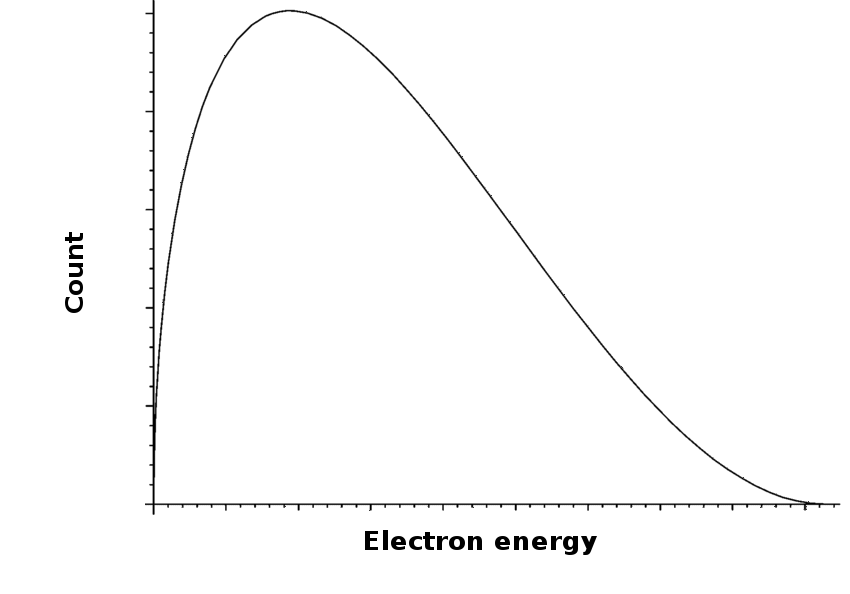
\includegraphics[width=0.5\textwidth,keepaspectratio]{beta_spectrum.png}
	        	\caption[Spectre de désintégration $\beta$.]{\label{fig::beta_spectrum}Spectre de l'énergie d'un électron émis par une désintégration $\beta$ d'énergie $Q$. Le fait qu'il soit continue entre 0 et $Q$ indique qu'une autre particule est émise en même temps que l'électron.}
	        \end{wrapfigure}
	        La désintégration $\beta$ est la transformation spontanée d'un neutron d'un noyau atomique en proton via l'émission d'un électron et d'un antineutrino électronique. L'énergie émise par une telle désintégration est égale, d'après la formule d'Einstein, à la différence des masses des noyaux avant et après désintégration multipliée par la vitesse de la lumière au carré : 
	        \begin{equation}
	        	Q = \left[m\left(^A_Z X\right)-m\left(^A_{Z+1} X\right)\right]c^2
	        \end{equation}
	        Pour un type de noyau $\left(^A_Z X\right)$, cette énergie est constante. La conservation de l'énergie nous dit alors que
	        \begin{equation}
	        	E_{initial} = E_{final} +E_{e^-}+E_{\overline{\nu}_e} = E_{final}+Q
	        \end{equation}
	        où $E_{initial}$ est l'énergie totale du noyau avant désintégration, $E_{final}$ est son énergie après désintégration et $E_{e^-}$ et $E_{\overline{\nu}_e}$ sont les énergies de l'électron et de l'antineutrino. On a donc $E_{e^-}+E_{\overline{\nu}_e} = Q$.
	        
	         Au moment de la proposition de l'existence du neutrino par Wolfgang Pauli en 1930\cite{Pauli1930}, seul l'électron et le noyau après désintégration étaient détectables, aussi le terme d'énergie $E_{\overline{\nu}_e}$ était absent de l'équation précédente. Dans ce cas, pour une source radioactive donnée, puisque $Q$ est constante, le spectre en énergie de l'électron aurait due être très piqué atour de $Q$. Or ce n'est pas le cas : ce spectre est continue (voir \autoref{fig::beta_spectrum}) entre 0 et $Q$. En revanche, rajouter à la réaction une particule jusque-là invisible correspond parfaitement à ce spectre, pourvu que la masse de cette particule soit très petite devant $Q$. En effet, si l'antineutrino (et donc le neutrino) avait une masse conséquente, le spectre de l'énergie de l'électron ne pourrait pas atteindre la valeur de $Q$, puisqu'un partie irréductible de $Q$ irait dans la masse du neutrino. C'est d'ailleurs un mesurant avec une très grande précision le spectre de l'énergie des électrons issues de la désintégration du tritium que l'expérience KATRIN\cite{Kleesiek2018} vise à déterminer la masse effective du neutrino électronique avec une précision de \SI{0.2}{\electronvolt\per c\squared}.
    
        \subsection{Premières observations directes du neutrino}
        
	        Entre les années 30 et 50, la détection du neutrino semblait hors de portée. Il était connu que la probabilité d'interaction de cette particule étant très faible, seule un source très intense de neutrinos pouvait permettre leur observation. Le développement de l'énergie nucléaire dans les années 50 a fourni cette source : les réactions de fission sont accompagnées de l'émission d'antineutrinos électroniques en très grande quantité.
	        
	        Entre 1952 et 1953, Frederick Reines et Clyde Cowan construisent un détecteur dont le matériau de réaction est simplement de l'eau. Un antineutrino incident, quand rencontre un proton, fait une réaction $\beta$ inverse produisant un neutron et un positron, se dernier s'annihilant rapidement avec un électron pour donner deux photons. Le signal attendu est alors la détection de deux photons suivie par l'interaction d'un neutron avec l'eau caractérisée par l'émission d'un troisième photon, après absorption du neutron par un noyau de chlorure de cadmium, un bon absorbeur de neutron que Reines et Cowan avaient dissous dans l'eau. La détection des photons s'effectuaient dans une couche de scintillateur liquide munie de tubes photomultiplicateurs entourant les deux cuves de détection. Le volume d'eau total était de $\SI{200}{\liter}$ où étaient dissous $\SI{40}{\kilogram}$ de chlorure de cadmium. Le flux de d'antineutrinos attendu du réacteur était de l'ordre de $\SI{e13}{\overline{\nu}_e\second^{-1}\centi\meter^{-2}}$.
	    
		    La première tentative de détection du neutrino fut faite proche du réacteur nucléaire de Hanford dans l'état de Washington, sans donner de résultat concluant. La seconde tentative, proche du réacteur de Savannah River en Caroline du Sud, détecta un signal de \SI{2.88}{\text{coups}\per\hour}\cite{Cowan1956} pour 1371 heures de prises de données, 20 fois supérieur au bruit de fond attendu, démontrant finalement l'existence d'une particule légère, et particulièrement peu réactive, dans la réaction $\beta$. La section efficace mesurée de  \SI{6.3e-44}{\centi\meter\squared} était compatible avec la valeur tirée des mesures de désintégration du neutron de Robson\cite{Robson1951}, de \SI{6e-44}{\centi\meter\squared}.
		    
		    Aujourd'hui, les expériences cherchant à détecter des neutrinos sont conçues de manière semblable à l'expérience de Reines et Cowan : un volume aussi grand et aussi dense que possible afin d'offrir un maximum de protons cibles sur lesquels les neutrinos  peuvent interagir, une source de neutrinos intense et un temps d'exposition long. La réduction du bruit de fond est essentielle dans une telle expérience : lors de leur seconde tentative, Reines et Cowan ont en effet placé leur détecteur sous terre. Ceci leur a permit de réduire grandement le taux de rayons cosmiques arrivant dans leur détecteur. En effet, ces derniers étaient susceptibles de créer des signaux semblables à celui attendu pour une interaction neutrino. Cette technique est encore largement employée aujourd'hui dans les expériences détectant des neutrinos.
		    
		    L'eau est encore utilisée aujourd'hui pour détecter des neutrinos, par exemple dans l'expérience Super-Kamiokande\cite{Fukuda1998}, mais des détecteurs solides ont également vu le jour comme dans les expériences NO$\nu$A\cite{Adamson2016} et OPERA\cite{Agafonova2018}. Une des techniques les plus récentes utilise comme cible des gaz nobles liquéfiés, plus dense que l'eau, notamment l'argon dans l'expérience prototype ICARUS\cite{Amerio2004} et la future expérience \gls{dune}\cite{Acciarri2016a}. 
		    
		    Les réacteurs nucléaires sont encore beaucoup utilisés dans les expériences de neutrinos, par exemple par Double Chooz\cite{Crespo-Anadon2014}, Daya Bay\cite{An2014}, RENO\cite{Collaboration2010} et la future JUNO\cite{An2015}. Les faisceaux de neutrinos créés artificiellement, plus contrôlables que les réacteurs, ont été inventés dans les années 60. L'expérience T2K\cite{Abe2018} détecte des neutrino issus d'un faisceau, et ce sera le cas également de l'expérience \gls{dune}\cite{Strait2016}. Des sources naturelles existent aussi : le soleil fourni un important flux de neutrinos, étudiés par des expériences comme SNO\cite{Aharmim2013}. Cette dernière, avec Super-Kamiokande\cite{Fukuda1998} qui détecte des neutrinos produits par des rayons cosmiques dans l'atmosphère, a permis de mettre en évidence le phénomène d'oscillation des neutrinos dont nous parlerons en détail dans la prochaine section. Les deux expériences ont reçu le prix Nobel de physique en 2015. Enfin, les neutrinos issus de supernovae peuvent également être détectés, pourvu qu'une supernovae explose durant une prise de données d'une expérience. C'est arrivé une seule fois en 1987, où 20 événements neutrinos ont été détectés par les détecteur IMB et Kamikande II\cite{Hirata1987}.

		\subsection{Les 3 familles de neutrinos}
		
			\begin{wrapfigure}{R}{0.5\textwidth}
				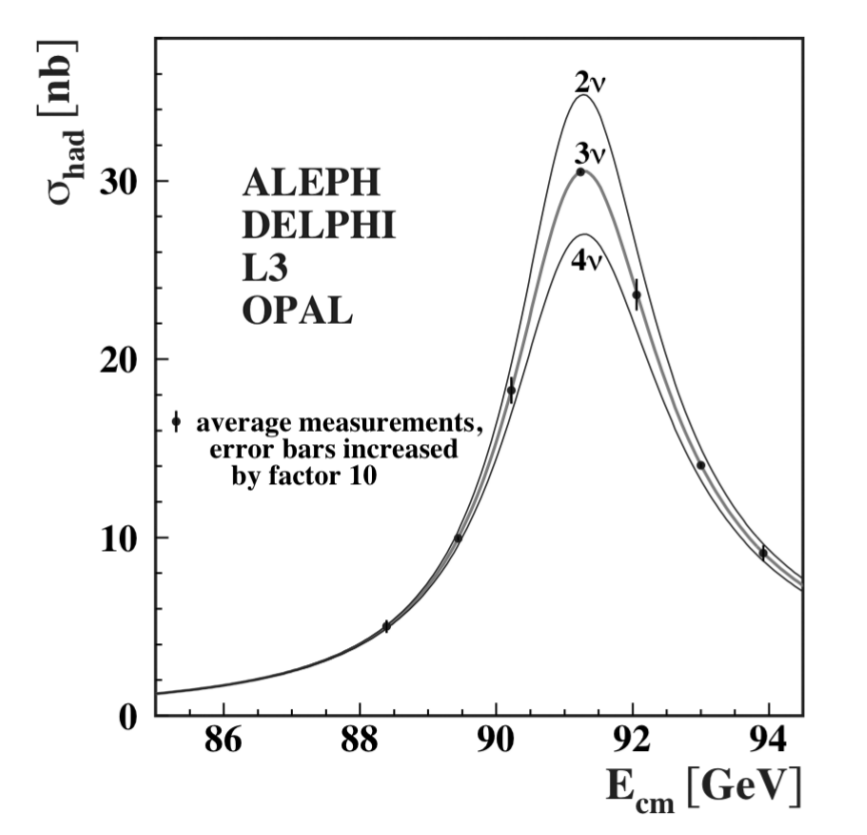
\includegraphics[width=0.5\textwidth,keepaspectratio]{three_neutrinos.png}
				\caption[Spectre de désintégration $\beta$.]{\label{fig::three_neutrinos}Mesure de la section efficace de production de hadron en fonction de l'énergie dans le centre de masse au LEP autour de la masse du boson $Z^0$. Résultats combinés des quatre expériences. Les courbes représentent les prédictions théoriques pour un nombre de saveurs de neutrinos actifs de 2, 3 et 4, les points sont les résultats de mesures, qui montre qu'il y a 3 familles de neutrinos actifs. Les incertitudes sont agrandies d'un facteur 10. Graphique tiré de \cite{Mele2015}.}
			\end{wrapfigure}
			Le muon, découvert en 1937 par Street et Stevenson\cite{Street1937}, n'a a priori comme différence avec l'électron que sa masse. Ce dernier étant (théoriquement, à l'époque) produit avec un neutrino dans les désintégrations $\beta$, il paraissait plausible que le muon puisse également être lié au neutrino d'une manière ou d'une autre.  Le spectre en énergie de l'électron produit par la désintégration du muon, mesuré par Leighton, Anderson et Seriff en 1949\cite{Leighton1949}, est continu. Un raisonnement identique à celui de Pauli de 1930 montre que le muon doit se désintégrer en trois particules : un électron et deux neutrinos. Il fallut cependant attendre 1962 et les expériences sur faisceau de neutrinos de Lederman, Steinberger et Schwartz\cite{Danby1962} pour détecter le neutrino muonique et définitivement montrer qu'il était différent du neutrino électronique : les neutrinos du faisceau, produits par la désintégration de muons, ne créaient que des muons dans le détecteur et aucun électron\footnote{Proche de la source, la probabilité  de changement de saveur lié au phénomène des oscillations des neutrinos est trop faible pour induire une composante autre que du neutrino muonique.}.
			
			La découverte du troisième lepton, le $\tau$, en 1975 par Perl\cite{Perl1975} n'a pas tardé à être suivi par la prédiction d'un troisième neutrino associé, le neutrino tauique. Ce dernier fut détecté en 2000 par l'expérience DONUT\cite{Collaboration2000}. Un faisceau de neutrinos issu du Fermilab, contenant toutes les saveurs possibles de neutrino, interagit avec un détecteur capable d'identifier les produits de réactions. Ce dernier a observé 4 événements neutrinos ayant créé un $\tau$.
			
			Les trois familles de quarks up--down, strange--charmed et top--bottom et les trois familles de leptons, l'électron et son neutrino, le muon et son neutrino et le tau et son neutrino, avaient alors été observées. Les quatre expériences du LEP, en étudiant la production de hadron à une énergie dans le centre de masse autour de la masse du boson $Z^0$, un des vecteurs de l'interaction faible, avait montré en 1989 qu'il ne pouvait pas exister plus de 3 saveurs de neutrinos sensibles à l'interaction faible\cite{DeCamp1989} (un graphique de cette étude est présenté en \autoref{fig::three_neutrinos}). Tous les neutrinos que nos instruments permettent de voir avaient alors été observés.
		    
		\subsection{Les symétries discrètes du modèle standard}\label{sec::CP}
		
			Un des principes fondamentaux du modèle standard, au même titre que la conservation de l'énergie, est que toute prédiction de ce dernier doit être identique après conjugaison Charge-Parité-Temps (CPT). Autrement dit, après avoir inversé la charge et les coordonnées spatio-temporelles.
			
			La conjugaison de charge inverse les charges -- électrique, isospin faible et couleur -- d'une particule. Un électron, par exemple, est transformé en positron, et de manière plus générale n'importe quelle particule chargée en son antiparticule. La transformation de parité consiste à prendre un système ou processus physique  et à le regarder dans un miroir. Autrement dit, remplacer toutes les coordonnées d'espace par leur opposées : $\Vec{r}\to-\Vec{r}$. Si la parité laisse le système ou processus inchangé, ce dernier est dit pair. Si au contraire il devient son opposé, il est dit impair. Un bon exemple de grandeur impaire est l'impulsion : $\Vec{p}(-\Vec{r}) = m(-\dot{\Vec{r}}) = -\Vec{p}(\Vec{r})$. À l'inverse, une grandeur paire est le moment cinétique : $\Vec{L}(-\Vec{r}) = -\Vec{r}\times -\Vec{p} = \Vec{L}(\Vec{r})$. L'extension à la mécanique quantique consiste à dire qu'un état est pair(impair) si il est état propre de l'opérateur de conjugaison de parité $\hat{P}$, qui inverse les coordonnées d'espace, avec une valeur propre de $+1(-1)$. Dans le modèle standard, une particule de spin $1/2$ est représentée par un spineur de Dirac $\psi(x,t)$, qui est composée de deux spineurs de Weyl :
			\begin{equation}
			\psi(x,t)=\left(\begin{matrix} u_R(x,t) \\ u_L(x,t)\end{matrix}\right)
			\end{equation}
			où $R$ et $L$ signifie "droite"(right) et "gauche"(left). Ils sont caractérisés par la manière dont un boost de Lorentz agit sur eux : ils acquièrent tous deux un facteur de phase, mais ces deux phases sont de signe opposé. Une transformation de parité transforme $u_R$ en $u_L$ et inversement. La dernière caractéristique importante d'un spineur de Weyl est qu'il est de masse nulle, alors qu'un spineur de Dirac peut avoir une masse $m_D$ : le lagrangien libre de Dirac, qui décrit comment évolue un spineur de Dirac sans interaction, autorise un terme de masse de la forme
			\begin{equation}\label{eq::dirac_mass}
			-m_D(\overline{u}_R u_L + \overline{u}_L u_R)
			\end{equation}
			où $\overline{u}_{R/L}$ est le conjugué de Dirac de $u_{R/L}$. Autrement dit, un fermion massif doit nécessairement avoir ses deux composantes gauche et droite non nulles. En revanche, il est possible qu'un fermion de masse nulle n'existe que dans un état de chiralité, gauche ou droite, auquel cas il peut être décrit par un spineur de Weyl $u_{R/L}$ seul. 
			
			La transformation de temps revient à inverser la flèche du temps et donc à regarder un processus dans l'autre sens. Par exemple, l'annihilation d'un électron avec un positron pour donner un photon devient l'émission d'une paire électron-positron par un photon.
			
			\begin{wrapfigure}{R}{0.5\textwidth}
				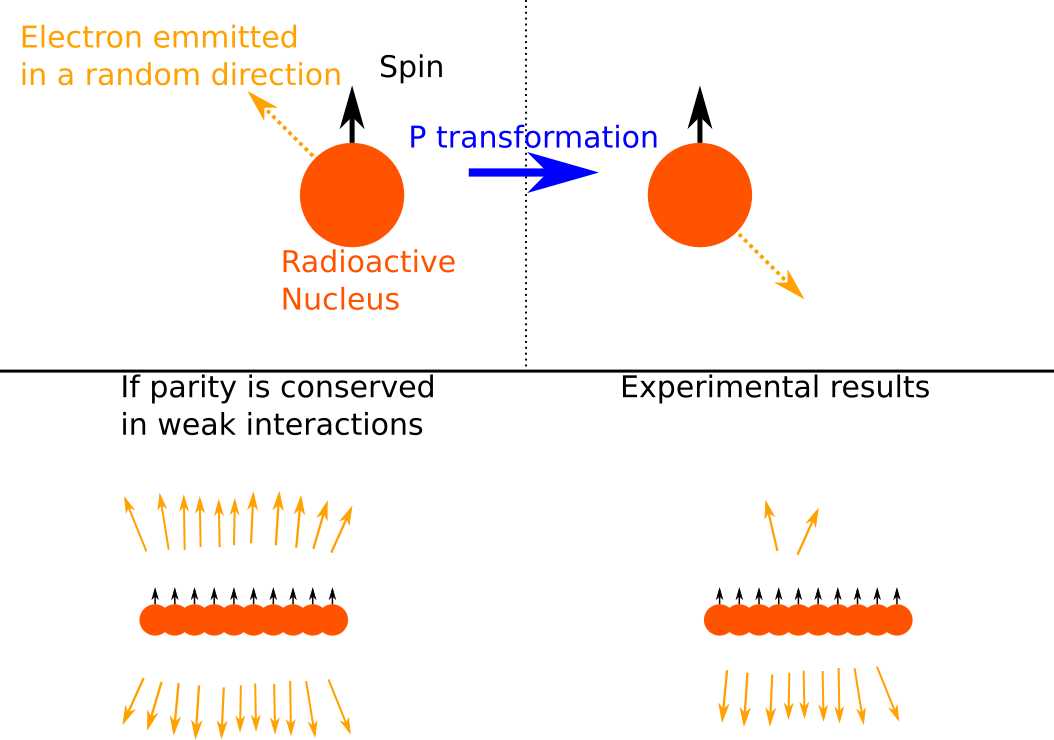
\includegraphics[width=0.5\textwidth,keepaspectratio]{wu2.png}
				\caption[Principe de l'expérience réalisée par C.S. Wu en 1957.]{\label{fig::wu}Principe de l'expérience réalisée par C.S. Wu en 1957 : un groupe de noyaux radioactif dont les spins sont tous orientés dans la même direction doivent émettre des électrons de manière isotrope si la conjugaison de partié est une symétrie de l'interaction faible. Il a été observer que les électrons étaient en majorité émis dans la direction opposée au spin, démontrant la violation de la symétrie $P$ par l'interaction faible.}
			\end{wrapfigure}
			Jusqu'en 1956, tous les processus physiques observés étaient invariants par transformation de parité, et cette dernière était considéré comme une symétrie de la nature. Mais cette même année, Tsung Dao Lee et Chen Ning Yang\cite{Lee1956} se rendent compte que, bien que bon nombre d'expériences montrent que les interactions forte et électromagnétique sont en effet symétriques par transformation de parité, aucune n'a étudié la question pour l'interaction faible. Ils proposent alors plusieurs méthodes expérimentales permettant de tester la conservation de la parité de l'interaction faible. L'une de ces expériences est réalisée entre 1956 et 1957 par Chieng-Shiung. Elle consiste à étudier la distribution spatiale des électrons émis par des noyaux radioactifs $\beta$ avec des spins alignés. La \autoref{fig::wu} schématise le signal recherché : le spin est invariant par transformation de parité alors que l'impulsion change de signe. L'image miroir d'un noyau émettant un électron dans la même direction que son spin est donc le même noyau émettant cet électron dans la direction opposée au spin. Le processus miroir est donc différent du processus initial et donc, pour que la désintégration $\beta$ soit symétrique par rapport à la transformation de parité, il faut qu'un ensemble de noyaux radioactifs dont les spins sont alignés émettent en moyenne autant d'électrons dans la direction de leur spin que dans la direction opposée. Or, l'expérience montre que ce n'est pas le cas : l'électron est en écrasante majorité émis dans la direction opposée au spin\cite{Wu1957}. L'interaction faible viole donc la symétrie $P$. Tsung Dao Lee et Chen Ning Yang reçoivent le prix Nobel en 1957 pour ces travaux.
			
			L'expérience de Wu, et plus tard celle de Goldhaber\cite{Goldhaber1958} en 1957, ont montré que l'interaction faible n'agit que sur la composante de chiralité gauche d'un spineur de Dirac, autrement dit la composante $\psi_L(x,t)=\left(\begin{matrix}0 \\ u_L(x,t)\end{matrix}\right)$. C'est pour cela qu'elle ne conserve pas la symétrie P. La masse du neutrino étant alors considérée comme nulle, il était naturel d'utiliser un spineur de Weyl de chiralité gauche pour décrire le neutrino, et un spineur de Weyl de chiralité droite pour décrire l'antineutrino.
			
			Si le neutrino est de charge nulle, une conjugaison de charge ne saurait le changer en son antineutrino. En effet, ce dernier n'existe que dans un état de chiralité droite, il faut donc également appliquer un transformation de parité. On peut donc se poser la question suivante : la transformation CP est-elle une symétrie du modèle standard? Si c'est le cas, les neutrinos et les antineutrinos doivent se comporter de la même manière. De manière générale, toute la matière décrite par le modèle standard se comporterait alors comme l'antimatière. Mais ceci soulève alors une question encore plus fondamentale : pourquoi n'y a-t-il plus d'antimatière dans l'univers? En effet, les théories actuelles du big bang\cite{Canetti2012} montrent qu' il devait y avoir autant de matière que d'antimatière à la création de l'univers. Matière et antimatière s'annihilent si elles se rencontrent, l'univers devrait être composé essentiellement de vide et de photons. Or ce n'est pas le cas : l'antimatière a disparu et la matière est restée. Le phénomène, appelé baryogenèse, responsable de cette asymétrie est encore mal connu, mais le fait que l'antimatière ne se comporte pas tout à fait comme la matière est nécessaire\cite{Sakharov1991}. Une telle asymétrie doit exister si la transformation CP n'est pas une symétrie de l'univers.
			
			Il a été expérimentalement prouvé que la symétrie CP n'est pas conservée dans le secteur des quark\cite{Collaboration2006,Charles2004,Kobayashi1973}: la matrice de mélange CKM contient une phase complexe introduisant un comportement légèrement différent entre les quarks et les antiquarks. Mais la violation de CP dans ce secteur n'est pas suffisante pour expliquer la baryogenèse\cite{Riotto1998}. En revanche, l'observation d'une violation de CP dans le secteur des leptons peut l'expliquer\cite{Davidson2008}. Comme nous le montrerons plus loin, le phénomène d'oscillation des neutrinos introduit également une phase complexe pouvant créer une différence de comportement entre matière et antimatière.
        
        \subsection{La masse du neutrino : Dirac ou Majorana}\label{sec::dirac_majorana}
        
	      \begin{activitybox}[label=box::mass_term]{Comment construire un terme de masse dans un lagrangien?}
	        	Le lagrangien du modèle standard est construit en utilisant le rasoir d'Ockham : on choisi en priorité les termes les plus simples qui respectent les lois de la physique. Un terme de masse doit donc respecter les critères suivants :
	        	\begin{itemize}
					\item[$\bullet$] Être invariant de Lorentz (i.e respecter la relativité restreinte).
					\item[$\bullet$] Avoir la dimension d'une énergie (le lagrangien est une énergie).
					\item[$\bullet$] Il doit faire intervenir la particule dont il est la masse.
					\item[$\bullet$] Il doit être réel, donc faire intervenir le champ et son conjugué complexe.
	        	\end{itemize}
	        	Le terme le plus simple respectant tous ces critères est, pour un fermion décrit par un champ $\psi$, de la forme $-m\bar{\psi}\psi$.
        	\end{activitybox}
	        
	        Nous avons vu dans la section précédente qu'un neutrino sans masse peut être décrit par un spineur de Weyl. Depuis la mise en évidence de la masse des neutrinos par le phénomène d'oscillation, il est clair que cette description est insuffisante, un spineur de Weyl ne pouvant pas avoir de terme de masse dans un lagrangien de Dirac. L'extension la plus simple consiste à considérer le neutrino comme un spineur de Dirac et de lui adjoindre le terme de masse \eqref{eq::dirac_mass} (voir l'encadré \ref{box::mass_term} pour une explication sur comment créer un terme de masse). Dans ce cas, le neutrino aura une composante de chiralité droite non nulle, qui n'interagit avec aucune interaction du modèle standard. Il peut interagir par gravitation, mais cette dernière est bien trop faible pour être détectable à l'échelle de la physique des particules. 
	        
	        Il existe une autre possibilité pour un terme de masse du neutrino: par son absence de charge, le neutrino peut également être décrit par un fermion de Majorana, dont le terme de masse est très différent de celui d'un fermion de Dirac. Un spineur de Majorana a la particularité qu'il est sa propre antiparticule. Dans le modèle standard, seul le neutrino peut être décrit par un spineur de Majorana. En effet, les autres fermions ont une charge électrique, ils ne peuvent donc pas être leur propre antiparticule qui doit être de charge opposée. Dans ce cas là, un nouvel état de chiralité droite n'est pas nécessaire, et donc aucun neutrino stérile n'est introduit (une discussion plus détaillée ce trouve ici\cite{Petcov2013}).
	        
	        Nous avons écrit en section précédente le terme de masse d'un spineur de Dirac. Pour un neutrino dans un état propre de l'hamiltonien $\nu_i=\nu_R+\nu_L$, nous avons donc : 
	        \begin{equation}
	        	-m_D\overline{\nu}_R \nu_L + \text{conjugué complexe}
	        \end{equation}
	        Ce terme de masse est créé, comme pour les autres fermions, par interaction du champ de neutrino avec le champ de Higgs après brisure de symétrie via un couplage de Yukawa. Il n'implique pas forcément de physique au-delà du modèle standard.
	        
	        Un terme de masse de Majorana quant à lui est de la forme
	        \begin{equation}\label{eq::majorana_mass}
	        -\frac{1}{2}m_M\overline{\nu}_L^T C \nu_L + \text{conjugué complexe}
	        \end{equation}
	        où $C$ est la matrice de conjugaison de charge. Comme l'explique B. Kayser dans \cite{Kayser2009}, un tel terme ne peut pas être créé par un couplage de Yukawa, mais par une interaction plus complexe avec le champ de Higgs qui n'est pas décrite par le modèle standard. Un terme de masse de Majorana pourrait expliquer la petitesse des masses des neutrinos par le mécanisme dit de see-saw , qui prédit l'existence de neutrinos ultra-lourds (\numprint{e9}--\SI{e15}{\giga\electronvolt}). Si la symétrie CP n'est pas conservée, ces derniers se seraient désintégrés à l'origine de l'univers en produisant un peu plus de matière que d'antimatière (voir l'article deB. Kayser\cite{Kayser2005}).
	        
	        Les différences de comportement entre neutrino de Dirac et de Majorana sont difficiles à observer. La plus recherchée en ce moment est la désintégration double-beta sans émission de neutrino, qui n'est possible que si le neutrino est sa propre antiparticule. Aucun résultat concluant n'a été observé à ce jour\cite{Dolinski2019}.
    
    \section{Le paradigme des oscillations des neutrinos}
    
        \subsection{Genèse de la théorie}
    
            On désigne habituellement un neutrino par sa saveur : neutrinos électronique ($\nu_e$), muonique ($\nu_{\mu}$) ou tauique ($\nu_{\tau}$). Quand un lepton chargé (électron muon ou tau) interagit avec un boson $W$, il se transforme en un neutrino de saveur définie (appelons-le $\nu_{\alpha}$), correspondant à celle du lepton chargé. De la même manière, un neutrino d'une saveur donnée (appelons-le $\nu_{\beta}$) se transforme en un lepton chargé de même saveur après interaction avec un boson $W$. Rien, à priori, n'oblige $\nu_{\alpha}$ à être de même saveur que $\nu_{\beta}$. Le premier à avoir soulevé ceci est Bruno Pontecorvo, même si il ne l'a pas fait en ces termes. En effet, au moment de la publication de ses deux premiers articles\cite{Pontecorvo:1957cp,Pontecorvo:1957qd} sur le sujet à la fin des années 60, seul le neutrino électronique avait été découvert. Pontecorvo parlait de possible transition entre neutrino et antineutrino du fait que le neutrino soit neutre, inspiré par les travaux de Gell-Mann et Païs\cite{Gell-Mann1955} sur la conversion du $\overline{K^0}$ en  $K^0$. Dans son article suivant en 1968\cite{Pontecorvo1968}, tout en gardant la possibilité de conversion des neutrinos vers les antineutrinos, il introduit la possibilité d'une conversion du neutrino électronique vers le neutrino muonique, découvert en 1962\cite{Danby1962}. Il prédira également deux résultats importants :
            \begin{itemize}
                \item[$\bullet$] Si les masses des neutrinos ne sont pas nulles et que la charge leptonique n'est pas conservée, les neutrinos peuvent changer de saveur.
                \item[$\bullet$] Dans ce cas, le flux de neutrino en provenance du soleil doit être environ 2 fois plus faible que le flux attendu sans changement de saveur.
            \end{itemize}
            La première prédiction implique de la physique au-delà du modèle standard, puisque ce dernier suppose que les masses des neutrinos sont nulles. La seconde prédiction fut vérifiée en 1970 par la Brookhaven Solar Neutrino Experiment\cite{Bahcall1976}, qui trouva un facteur de déficit compris entre 2 et 3. Il ne s'agissait alors pas encore d'une preuve, d'autres théories pouvant expliquer ce phénomène. Les auteurs de \cite{Bahcall1976} font d'ailleurs part de leur doutes quant à la précision des modèles solaires utilisés. Néanmoins, ce résultats était un indice qui a incité les chercheurs à creuser la question.
            
            Le changement de saveur $\nu_e\rightleftharpoons\nu_{\mu}$ avait été envisagé également entre 1962 et 1963 par deux groupes de physiciens, Katayama, Matumoto, Tanaka et Yamada\cite{Nakagawa1963} puis par Maki,  Nakagawa et  Sakata\cite{Maki1962}. Ces quatre derniers donneront leurs noms, avec Pontecorvo, à la célèbre matrice \gls{pmns} décrite plus loin, qui gouverne les transitions de saveur des neutrinos. Leur point de départ était différent de celui de Pontecorvo, puisqu'ils visaient à créer une théorie unifiant les leptons et les hadrons. Ils sont également arrivés à la conclusion qu'un changement de saveur des neutrinos implique que ces derniers doivent avoir des masses non nulles.
            
            En 2015, Arthur~B.~McDonald et Takaaki Kajita ont reçu le prix Nobel de physique "pour la découverte des oscillations des neutrinos, qui montre que les neutrinos ont une masse". Les deux expériences ayant fait cette découverte sont SNO\cite{Aharmim2013} et Super-Kamiokande\cite{Fukuda1998}.
            
            \begin{figure}[htbp]
                \begin{subfigure}[t]{0.56\textwidth}
                    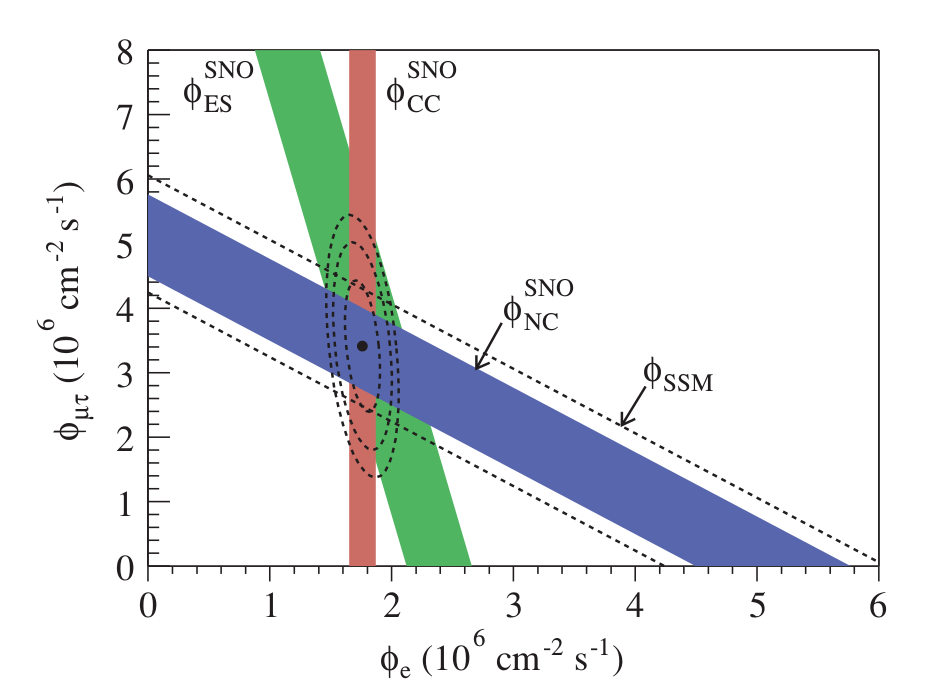
\includegraphics[width=\textwidth]{Chapitre_1/pictures/SNO_plot.png}
                    \caption{Composition $\nu_{\mu}$ et $\nu_{\tau}$ du flux des neutrinos solaires $^8$B en fonction de sa composition en $\nu_e$\cite{Aharmim2013}. La prédiction du modèle solaire est $\phi_{e}=\SI{5.15e6}{\nu\per\centi\meter\per\second}$. Les traits pointillés indiquent alors les valeurs possibles $\phi_{\mu\tau}$ et $\phi_e$ si les neutrinos peuvent changer de saveurs. Le flux mesuré par courant chargé $\phi_{CC}^{SNO}$ n'est sensible qu'aux $\nu_e$ et est donc égal à $\phi_{e}$. SNO l'a mesuré autour de $\SI{1.76e6}{\nu\per\centi\meter\per\second}$ (bande verticale rouge). Le flux mesuré par diffusion élastique $\phi_{ES}^{SNO}$ est égal à $\phi_{e}+0.1559\phi_{\mu\tau}$ (bande verte). SNO l'a mesuré autour de $\SI{2.39e6}{\nu\per\centi\meter\per\second}$. Le flux de courant neutre $\phi_{NC}^{SNO}$ est sensible de manière égale aux trois saveurs et est donc égal à $\phi_{e}+\phi_{\mu\tau}$, soit au flux total attendu. SNO le mesure autour de $\SI{5.09e6}{\nu\per\centi\meter\per\second}$, compatible avec la prédiction. Le fait que ces trois bandes s'interceptent en un même point indique que le flux total de neutrinos est en accord avec la prédiction, mais qu'il n'est pas composé uniquement de $\nu_e$, indiquant un changement de saveur.}
                    \label{fig::SNO_plot}
                \end{subfigure}
                \hfill 
                \begin{subfigure}[t]{0.4\textwidth}
                    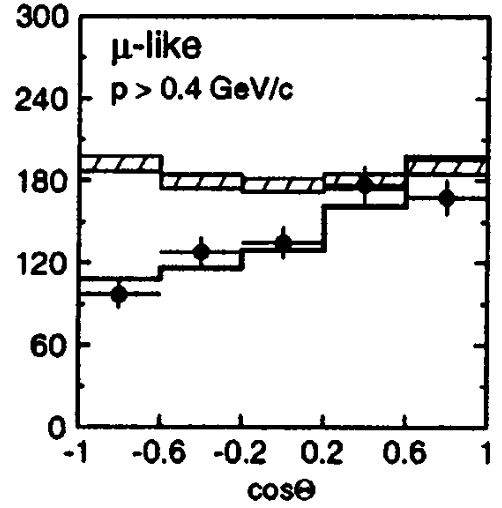
\includegraphics[width=\textwidth]{Chapitre_1/pictures/superK_plot.png}
                    \caption{Nombre de neutrinos muoniques mesurés par Super-Kamiokande (traits pleins) et prédit par le Monte Carlo en l'absence de changement de saveur (surfaces hachurées) pour un an et demi de prise de donnée, en fonction l'angle entre la verticale et la direction du neutrino\cite{Fukuda1998}. Un cosinus négatif correspond à un neutrino ayant traversé la Terre. La différence entre observation et prédiction à grand angle indique une disparition des neutrinos muonique à grande ligne de base.}
                    \label{fig::superK_plot}
                \end{subfigure}
                \caption[Les preuves que les neutrinos changent de saveur, par SNO et Super-Kamiokande.]{Les deux graphiques ayant prouvé les changement de saveur des neutrinos : le flux total de neutrinos provenant du soleil est conservé mais sa composition de saveur change, par SNO (gauche). Le nombre de neutrinos muoniques atmosphériques détectés dépend de la ligne de base, par Super-Kamiokander (droite).}
            \end{figure}
            
            SNO détectait les neutrinos solaires, par interaction par courant chargé (CC) et par courant neutre (CN), permettant d'avoir accès à la fois au flux de neutrinos électroniques (CN et CC) et au flux de neutrios muoniques et tauiques (CN). Comme le montre la \autoref{fig::SNO_plot}, la somme des trois flux correspond bien au flux total prédit par le modèle solaire standard alors que le flux de neutrinos électroniques est inférieur aux prédictions, montrant qu'une partie du flux change de saveur mais que le flux total est conservé.
            
            Super-Kamiokande détecte des neutrinos issus des interactions de rayons cosmiques avec l'atmosphère. Il pouvait ainsi comparer les flux des neutrinos pour différents angles zénithaux, correspondant à des créations du neutrino allant de juste au dessus du détecteur (angle nul) à l'autre bout du globe (angle de $\pi$). Comme nous allons le montrer plus loin, la probabilité qu'a un neutrino de changer de saveur dépend de la distance parcourue (équation \eqref{eq::proba_oscillation}). Une dépendance du flux en l'angle zénithal a donc indiqué un phénomène de changement de saveur dépendant de la distance. La \autoref{fig::superK_plot} montre cette dépendance pour des détections de neutrinos muoniques.
    
        \subsection{Pourquoi "Oscillations"?}\label{sec::oscillations}
            La base de la théorie des changements de saveur des neutrinos est de dire que les états $\nu_e$ $\nu_{\mu}$ et $\nu_{\tau}$ sont -- par définition -- des états propres du lagrangien d'interaction, mais pas forcément des états propres de l'hamiltonien, appelés également états propres de masse. Autrement dit, les états propres de saveur sont une composition linéaire des états propres de masse, et inversement. Il n'est donc pas possible de décrire la propagation dans l'espace-temps d'un état de saveur, bien que le neutrino soit créé et détruit dans un de ces états. Partant de là, nous allons montrer d'où provient le terme "oscillation".
            
            \subsubsection{Conventions de notation}
            \begin{itemize}
                \item[$\bullet$] $\hbar = c = 1$ (système d'unité naturelle)
                \item[$\bullet$] Nous supposerons que toutes les fonctions d'ondes décrites sont suffisamment loin de leur source pour être considérées comme des ondes planes. Les expériences de neutrinos vérifient généralement facilement cette condition.
                \item[$\bullet$] $\nu_e$, $\nu_{\mu}$ et $\nu_{\tau}$ sont les états propres de saveur. Un neutrino est dans un de ces états au moment de son interaction.
                \item[$\bullet$] $\nu_{\alpha,\beta...}$ désigne un des trois états propres de saveur.
                \item[$\bullet$] $l_{\alpha,\beta...}$ désigne un des trois leptons chargés $e$, $\mu$ ou $\tau$.
                \item[$\bullet$] $U_{\alpha i}$ est un élément de la matrice $U$ permettant de passer de la base des états propres de saveur à la base des états propres de masse.
                \item[$\bullet$] $\nu_{i}$ avec $i$ un entier non nul désigne un état propre de masse, qui vérifie l'équation
                \begin{equation}
                    \ket{\nu_i(t)} = e^{-i(E_i\cdot t - p_i\cdot x)}\ket{\nu_i(0)}.
                \end{equation}
                avec $E_i$ et $p_i$ l'énergie et l'impulsion du neutrino, constantes au cours du temps.
            \end{itemize}
            
            \subsubsection{Superposition des états de masse}
            Les états propres de saveurs, si ils ne sont pas des états de masses, sont une superposition linéaire de ces états. On peut donc écrire
            \begin{eqnarray}
            \ket{\nu_{\alpha}} = \sum_i U_{\alpha i}^*\ket{\nu_i} \label{eq::alphatoi} \\
            \ket{\nu_i} = \sum_{\alpha} U_{\alpha i}\ket{\nu_{\alpha}}.
            \end{eqnarray}
            L'état d'un neutrino initialement créé dans une saveur $\alpha$ est alors :
            \begin{equation}
            	\ket{\nu(t=0)} = \ket{\nu_{\alpha}} = \sum_i U_{\alpha i}^*\ket{\nu_i(t=0)}
            \end{equation}
            Son état à un temps $t > 0$ est alors :
            \begin{equation}\label{eq::0tot}
	            \begin{split}
	            	\ket{\nu(t)} &=\sum_{i} U_{\alpha i}^*\ket{\nu_i(t)} = \sum_{i} U_{\alpha i}^* e^{-i(E_i\cdot t - p_i\cdot x)}\ket{\nu_i(0)} = \sum_{i} U_{\alpha i}^* e^{-i(E_i\cdot t - p_i\cdot x)}\sum_{\beta}U_{\beta i}\ket{\nu_{\beta}}\\ & = \sum_{i,\beta} U_{\alpha i}^*U_{\beta i} e^{-i(E_i\cdot t - p_i\cdot x)}\ket{\nu_{\beta}}
            	\end{split}
            \end{equation}
            
            Plusieurs points méritent d'être soulignés ici :
            \begin{itemize}
                \item[$\bullet$] Un état de saveur $\alpha$ ne peut se transformer qu'en un lepton de même saveur. Les états de saveur doivent donc être orthogonaux.
                \item[$\bullet$] Il a été montré expérimentalement qu'il ne peut exister que trois états de saveurs actives (i.e sensibles à l'interaction faible)\cite{pdg2018} de masse inférieure à la moitié de celle du boson $Z^0$. Il faut donc au moins trois états de masse. Si il existe plus de trois états de masse, il doit alors exister d'autres états, soit plus lourds que le $Z^0$, soit insensibles à l'interaction faible, soit les deux. Ceci ne sont pas prédits par le modèle standard et pourraient constituer une partie de la matière noire.
                \item[$\bullet$] La matrice $U$ étant une matrice de changement de base, elle doit être unitaire :
                \begin{equation*}
                    \delta_{\alpha\beta} = \braket{\nu_{\alpha}}{\nu_{\beta}} = \braket{\sum_i U_{\alpha i}\nu_i}{\sum_j U_{\beta j}^*\nu_j} = \sum_{i,j} U_{\alpha i}U_{\beta j}^* \braket{\nu_i}{\nu_j} = \sum_{i,j} U_{\alpha i}U_{\beta j}^*.
                \end{equation*}
            \end{itemize}
            Comme nous ne pouvons détecter que les trois états de saveur $\nu_e$, $\nu_{\mu}$ et $\nu_{\tau}$, il convient de travailler avec un matrice $3\times3$. La combinaison des mesures actuelles et futures des éléments de cette matrice\cite{Qian2013} permettra de tester si cette matrice est unitaire. Si ce n'est pas le cas, cela prouvera l'existence d'états de saveurs encore non observés car alors la matrice $3\times3$ ne sera qu'une sous-matrice d'une matrice plus grande qui, elle, doit être unitaire.
            
            Avant de détailler cette matrice $U$, intéressons-nous à la probabilité de changement de saveur.
             
            \subsubsection{Quelle est la probabilité de passer d'une saveur $\beta$ vers une saveur $\alpha$?}\label{sec::proba_oscillations}
            En notant $\ket{\nu(t)}$ l'état de masse dans lequel se trouve un neutrino à un instant $t$ , cette probabilité est donnée par la projection de l'état de saveur $\beta$ sur cet état :
            \begin{equation}
                P(\nu_{\alpha}\to\nu_{\beta})=\bigg|\braket{\nu_{\beta}}{\nu(t)}\bigg|^2.
            \end{equation}
            En utilisant les équations \eqref{eq::alphatoi} et \eqref{eq::0tot} on montre que
            \begin{equation}
                \braket{\nu_{\beta}}{\nu(t)} = \sum_i U_{\alpha i}^*U_{\beta i} e^{-i(E_i\cdot t - p_i\cdot x)}.
            \end{equation}
            Ici aussi plusieurs choses sont à noter : 
            \begin{itemize}
                \item[$\bullet$] $t$ correspond au temps écoulé entre la création et la disparition du neutrino dans le référentiel du détecteur. Ce temps n'est généralement pas mesurable.%, étant donné que les sources de neutrinos en émettent continuellement. Impossible donc de savoir à quel moment a été émis le neutrino détecté.
                \item[$\bullet$] $x$ correspond à la distance parcourue par le neutrino. Nous la noterons $L$ dans la suite du texte et l'appellerons \textit{ligne de base}. Elle est mesurable puisque c'est la distance entre la source et le détecteur.
                \item[$\bullet$] De part leur masse très faible, les neutrinos que nous détectons sont ultra-relativistes. On peut donc faire l'approximation $p_i \simeq E_i - \frac{m_i^2}{2E_i}$.
            \end{itemize}
            
            \begin{wrapfigure}{R}{0.48\textwidth}
            	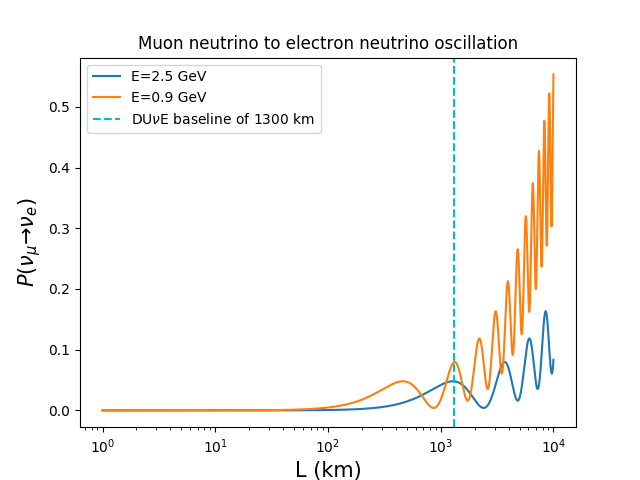
\includegraphics[width=0.48\textwidth,keepaspectratio]{numu-nue-vs-L-3flav.png}
            	\caption[$P(\nu_{\mu}\to\nu_e)$ en fonction de $L$]{$P(\nu_{\mu}\to\nu_e)$ en fonction de $L$. fonction de $L$ pour un neutrino de \SI{0.9}{\giga\electronvolt} et \SI{2.5}{\giga\electronvolt}. La ligne verticale représente la ligne de base de \gls{dune}. Le faisceau de neutrino envoyé aura des énergies allant de \SI{0.5}{\giga\electronvolt} et \SI{5}{\giga\electronvolt}, incluant donc les deux premiers maxima locaux de probabilité.}
            	\label{fig::3flavors_oscillations}
            \end{wrapfigure}
            Dans une expérience détectant des neutrinos, la probabilité sera moyennée sur le temps $t$, inconnu. Supposons que la source des neutrinos ait deux composantes d'énergies différentes $E_1$ et $E_2$, contribuant de manière cohérente au signal observé dans le détecteur. Au bout du temps $t$, chaque composante aura pris un facteur de phase $e^{-iE_jt}$. Les interférences entre les deux composantes feront alors entrer en jeu un facteur de phase $e^{-i(E_1-E_2)t}$. Moyenné sur $t$, ce facteur disparaît, sauf si $E_1 = E_2$. Les seules composantes contribuant de manière cohérente au signal ont donc une même énergie $E$. Ce point est détaillé dans les articles de Stodolsky\cite{Stodolsky1998}, Lipkin\cite{Lipkin2005} et Kayser\cite{Kayser2005}. On se retrouve donc avec l'équation suivante : 
            \begin{equation*}
                P(\nu_{\alpha}\to\nu_{\beta}) = \bigg|\sum_i U_{\alpha i}^*U_{\beta i} e^{-im_i^2\frac{L}{2E}}\bigg|^2.
            \end{equation*}
            Cette expression peut se mettre sous forme sinusoïdale\cite{Mondal2015} :
            \begin{equation}\label{eq::proba_oscillation}
                \begin{split}
                    P(\nu_{\alpha}\to\nu_{\beta}) = \delta_{\alpha\beta} & - 4\sum_{i>j}\Re(U_{\alpha i}U_{\beta i}^*U_{\alpha j}^*U_{\beta j})\sin^2\left(\Delta m_{ij}^2\frac{L}{4E}\right) \\
                    & +2\sum_{i>j}\Im(U_{\alpha i}U_{\beta i}^*U_{\alpha j}^*U_{\beta j})\sin\left(\Delta m_{ij}^2\frac{L}{2E}\right)
                \end{split}
            \end{equation}
            où $\Delta m_{ij}^2 = m_i^2-m_j^2$. Il peut être utile de définir une longueur d'oscillation $l_{osc} = 4\pi E/\Delta m_{ij}^2$ si l'on souhaite étudier les oscillations en fonction de la ligne de base $L$ pour des énergies fixées, réécrivant alors les termes en $\sin$ et $\sin^2$ :
            \begin{eqnarray}
                \sin^2\left(\Delta m_{ij}^2\frac{L}{4E}\right) = &  \sin^2\left(\pi\frac{L}{l_{osc}}\right) \\
                \sin\left(\Delta m_{ij}^2\frac{L}{2E}\right) = & \sin\left(2\pi\frac{L}{l_{osc}}\right).
            \end{eqnarray}
                        
            On peut noter trois choses:
            \begin{itemize}
                \item[$\bullet$] Le terme "oscillation" est ici évident : la probabilité qu'a un neutrinos de changer de saveur est une fonction sinusoïdale du ratio $\frac{L}{E}$. L'exemple du changement de saveur $P(\nu_{\mu}\to\nu_e)$, important pour les expériences comme \gls{dune} détectant des neutrinos issus de faisceaux, est illustré en \autoref{fig::3flavors_oscillations}.
                \item[$\bullet$] La masse d'un neutrino ne sera pas accessible par la mesure de probabilité d'oscillation : seule une différence de masse au carré est accessible. On ne peut donc pas, avec les oscillations des neutrinos, déterminer les valeurs des masses des neutrinos.
                \item[$\bullet$] Si les neutrinos ont des masses nulles ou égales, les termes en $\Delta m_{ij}^2$ s'annulent et les probabilités de transitions sont nulles. L'observation du phénomène d'oscillation des neutrinos montre donc bien que deux masses au moins sont non nulles.
                \item[$\bullet$] La somme $\sum_{\beta\in\{e,\mu,\nu\}}P(\nu_{\alpha}\to\nu_{\beta})$ doit être égale à 1 de par l'unitarité de $U$. Les neutrinos ne disparaissent pas entre leur émission et leur arrivée au détecteur\footnote{Leurs sections efficaces d'interaction sont trop faibles pour impacter le flux mesuré.}, ils changent de saveur. Mais si une de ces saveurs n'est pas observable parce que stérile, alors le flux total observable s'en verra diminué. Les résultats de SNO montrés en \autoref{fig::SNO_plot} tendent à montrer que la probabilité d'osciller vers un tel état est faible, au moins aux valeurs de $L/E$ correspondant aux neutrinos solaires.
            \end{itemize}
            
            On peut immédiatement calculer la même probabilité pour les antineutrinos, en supposant que la symétrie CPT n'est pas violée : 
            \begin{equation}
                P(\overline{\nu}_{\alpha}\to\overline{\nu}_{\beta}) = P(\nu_{\beta}\to\nu_{\alpha}).
            \end{equation}
            La partie réelle de l'équation \eqref{eq::proba_oscillation} restera inchangée, tandis que la partie imaginaire deviendra négative. On aura donc :
            \begin{equation}
                \begin{split}
                    P(\overline{\nu}_{\alpha}\to\overline{\nu}_{\beta}) = \delta_{\alpha\beta} & - 4\sum_{i>j}\Re(U_{\alpha i}U_{\beta i}^*U_{\alpha j}^*U_{\beta j})\sin^2\left(\Delta m_{ij}^2\frac{L}{4E}\right) \\
                    & -2\sum_{i>j}\Im(U_{\alpha i}U_{\beta i}^*U_{\alpha j}^*U_{\beta j})\sin\left(\Delta m_{ij}^2\frac{L}{2E}\right).
                \end{split}
            \end{equation}
            Et donc, si le dernier terme est différent de 0, les neutrinos et les antineutrinos se comportent différemment, montrant que la symétrie CP est brisée dans le modèle standard.
            
            Tous les calculs ont été fait en unités naturelles $\hbar = c = 1$. Il convient de repasser en unités SI si on veut pouvoir prédire des grandeurs mesurables. Une rapide analyse dimensionnelle montre que 
            \begin{eqnarray}
                \Delta m_{ij}^2\frac{L}{4E}(nat.)
                = \Delta m_{ij}^2\frac{L}{4E}\frac{c^3}{\hbar}(SI)
                \simeq \numprint{1.27}\Delta m_{ij}^2(\si{\electronvolt\squared})\frac{L(\si{\kilo\meter})}{E(\si{\giga\electronvolt})} \\ 
                l_{osc}(\si{\kilo\meter}) = \frac{4\pi E\hbar}{\Delta m_{ij}^2c^3} \simeq \numprint{2.48}\frac{E(\si{\giga\electronvolt})}{\Delta m_{ij}^2(\si{\electronvolt\squared})}.
            \end{eqnarray}
            
        \subsubsection{Deux cas particuliers}
            Deux cas particuliers et faciles à traiter sont les oscillations à deux saveurs, qui étaient de bonnes approximations pour les premières expériences de mesure de probabilité d'oscillation, et la probabilité de conservation, i.e $P(\nu_{\alpha}\to\nu_{\alpha})$.
            
            Commençons par le cas de conservation. L'équation \eqref{eq::proba_oscillation} nous donne :
            \begin{equation}\label{eq::proba_non_oscillation}
                \begin{split}
                    P(\nu_{\alpha}\to\nu_{\alpha}) = 1 & - 4\sum_{i>j}\Re(U_{\alpha i}U_{\alpha i}^*U_{\alpha j}^*U_{\alpha j})\sin^2\left(\Delta m_{ij}^2\frac{L}{4E}\right) \\
                    & + 2\sum_{i>j}\Im(U_{\alpha i}U_{\alpha i}^*U_{\alpha j}^*U_{\alpha j})\sin\left(\Delta m_{ij}^2\frac{L}{2E}\right) \\
                    = 1 & -4\sum_{i>j}\Re(|U_{\alpha i}|^2|U_{\alpha j}|^2)\sin^2\left(\Delta m_{ij}^2\frac{L}{4E}\right).
                \end{split}
            \end{equation}
            Le terme contenant la partie imaginaire de l'équation \eqref{eq::proba_oscillation} ayant disparu, cette probabilité sera la même pour les antineutrinos. Il n'est donc pas possible de mesurer l'asymétrie matière-antimatière avec cette probabilité. Le terme oscillant étant en $\sin^2$, il n'est pas possible non plus de déterminer le signe de $\Delta m_{ij}^2$ en mesurant cette probabilité.
            
            Le cas des oscillations à deux saveurs, correspondant à une probabilité négligeable d'osciller vers la troisième saveur, s'obtient facilement en fixant $n=2$. Dans ce cas la matrice $U$ est une simple matrice de rotation à deux dimensions, réelle, avec un paramètre $\theta$ :
            \begin{equation}\label{eq::two_flavor_pmns}
                U = \left(\begin{matrix}
                    \cos(\theta) & \sin(\theta) \\
                    -\sin(\theta) & \cos(\theta)
                \end{matrix}\right)
            \end{equation}
            et la probabilité \eqref{eq::proba_oscillation} devient
            \begin{eqnarray}
                \label{eq::two_flavors}
                P(\nu_{\alpha}\to\nu_{\beta}) = \sin^2(2\theta)\sin^2\left(\frac{\Delta m^2 L}{4E}\right) \\ 
                \label{eq::two_flavors_length}
                P(\nu_{\alpha}\to\nu_{\beta}) = \sin^2(2\theta)\sin^2\left(\pi\frac{L}{l_{osc}}\right) \\
                \label{eq::two_flavors_survival}
                P(\nu_{\alpha}\to\nu_{\alpha}) = 1- \sin^2(2\theta)\sin^2\left(\pi\frac{L}{l_{osc}}\right)
            \end{eqnarray}
            avec bien entendu $\alpha\ne \beta$ (il suffit de prendre 1 moins cette probabilité pour avoir la probabilité de conservation). Ici aussi, la violation de CP n'est pas accessible, il n'y aura pas de différence matière-antimatière. Due au carré du sinus, cette probabilité n'est pas sensible non plus au signe de $\Delta m^2$. Le terme en $\sin^2(2\theta)$ correspond à l'amplitude d'oscillation, c'est à dire la fraction maximale de neutrinos $\alpha$ pouvant se changer en neutrinos $\beta$. $l_{osc}$ correspond ici a la distance entre deux maxima ou minima de probabilité de transition.
            
            Dans quels cas cette approximation est-elle valide? Il se trouve que les mesures actuelles ont montré que la différence des masses carrés entre les deux premiers états propres est 300 fois plus faible que les deux autres : 
            \begin{equation}
                |\Delta m^2_{21}| << |\Delta m^2_{31}| \simeq |\Delta m^2_{32}|.
            \end{equation}
            De plus, un autre résultat est que le terme $U_{e3}$ est très petit devant 1. Ces deux résultats permettent dans de nombreux cas d'approximer les oscillations à trois saveurs par une oscillation à deux saveurs.
            
            La première approximation qui peut être faite est pratique pour les expériences de neutrinos atmosphériques, de réacteurs et d'accélérateurs à faible et moyenne ligne de base. Dans ces cas, $L/E$ vérifie
            \begin{equation}\label{eq::approx_21_0}
                \Delta m^2_{21}\frac{L}{2E} << 1.
            \end{equation}
            et tous les termes en $\sin$ et $\sin^2$ dépendant de $\Delta m^2_{21}$ tendent vers 0. La probabilité de transition $\nu_{\alpha}\to\nu_{\beta}$ devient alors
            \begin{equation}
                P(\nu_{\alpha}\to\nu_{\beta}) = 4|U_{\alpha 3}|^2|U_{\beta 3}|^2\sin^2\left(\Delta m^2_{31}\frac{L}{4E}\right).
            \end{equation}
            qui est exactement la probabilité de transition dans l'approximation à deux saveurs \eqref{eq::two_flavors} si l'on identifie $4|U_{\alpha 3}|^2|U_{\beta 3}|^2=\sin^2(2\theta)$.
            
            La seconde approximation est utile lors de l'étude des neutrinos solaires et des expériences à très longue ligne de base. Dans ces cas, $L/E$ est trop grand pour que \eqref{eq::approx_21_0} soit vraie. En revanche, les relations suivantes sont vérifiées : 
            \begin{equation}\label{eq::approx_31_eq_32}
                \Delta m^2_{31}\frac{L}{2E} \simeq \Delta m^2_{32}\frac{L}{2E}  >> 1.
            \end{equation}
            Dans ce cas les oscillations dues à $\Delta m^2_{31}$ et $\Delta m^2_{32}$ sont tellement rapides qu'elles donnent lieu à un effet moyen qui donne comme probabilité de survie du neutrino électronique
            \begin{equation}
                P(\nu_e\to\nu_e) \simeq \sin^4(\theta_{13}) + \cos^4(\theta_{13})\left(1-\sin^2(2\theta_{12})\sin^2\left(\Delta m^2_{21}\frac{L}{4E}\right)\right)
            \end{equation}
            où les angle $\theta_{13}$ et $\theta_{12}$ sont introduits dans la section suivante et correspondent à $\sin(\theta_{13})=U_{e3}$ et $\sin(\theta_{12})\cos(\theta_{13})=U_{e2}$.
            
            Il est immédiat alors que si l'approximation 
            \begin{equation}\label{eq::approx_13_eq_0}
                U_{e3} << 1
            \end{equation}
            est valide, l'équation précédente devient
            \begin{equation}\label{eq::solar_oscillation}
                P(\nu_e\to\nu_e) \simeq 1-\sin^2(2\theta_{12})\sin^2\left(\Delta m^2_{21}\frac{L}{4E}\right).
            \end{equation}
            qui correspond à la probabilité de survie à deux saveurs \eqref{eq::two_flavors_survival}.
            
            Ces différentes approximations ont été utilisées dans la plupart des expériences d'oscillation des neutrinos jusqu'à aujourd'hui. Le défi des expériences les plus récentes et des expériences futurs est d'être sensible aux effets au delà de ces approximations, car ces effets peuvent contenir de la physique au delà du modèle standard comme nous allons le voir plus tard.
            
        \subsection{La matrice PMNS}\label{sec::pmns}
            \subsubsection{Généralités}
            Il est temps de décrire un peu plus en détail la $U$, également appelé matrice \gls{pmns}. Elle est de la forme : 
            \begin{equation}
                \left(\begin{matrix}
                     \nu_e \\ \nu_{\mu} \\ \nu_{\tau} \\ ...
                \end{matrix}\right) =
                \underbrace{\left(\begin{matrix}
                    U_{e1} & U_{e2} & U_{e3} & ... \\
                    U_{\mu 1} & U_{\mu 2} & U_{\mu 3} & ... \\
                    U_{\tau 1} & U_{\tau 2} & U_{\tau 3} & ... \\
                    ... & ... & ... &
                \end{matrix}\right)}_U
                \left(\begin{matrix}
                     \nu_1 \\ \nu_2 \\ \nu_3 \\ ...
                \end{matrix}\right)
            \end{equation}
            où les pointillés soulignent le fait que cette matrice n'est pas forcément $3\times 3$. Cette matrice représente une matrice de changement de base, équivalente à une matrice de rotation complexe à $n$ dimensions. Une telle matrice peut se représenter comme un produit de $\frac{n}{2}(n-1)$ matrices de rotation dans un plan donné\cite{Valle2006,Harari1986} : 
            \begin{equation}\label{eq::compact_pmns}
                U=u_0(\gamma)\prod_{i<j}^n u_{ij}
            \end{equation}
            où $u_0(\gamma)=e^{i \sum_{i}^{n}\gamma_i \mathbb{I}}$ est une matrice diagonale unitaire arbitraire ($\gamma$ est un vecteur quelconque) et $u_{ij}$ est une matrice de rotation telle que
            \begin{equation}
                \begin{split}
                    u_{ij}= & e^{\sum_{i=1}^n\left(\eta_{ij}A_i^j-\eta_{ij}^*A_j^i\right)},\\
                    \eta_{ij} = & \theta_{ij}e^{i\phi_{ij}},\\
                    \left(A_i^j\right)_k^l = & \delta_{ik}\delta_{jl}.
                \end{split}
            \end{equation}
            
            Par exemple, la matrice de rotation dans la plan $12$ sera
            \begin{equation}
                u_{12} = 
                \left(\begin{matrix}
                    \cos(\theta_{12}) & e^{i\phi_{12}}\sin(\theta_{12}) & 0 & ... \\
                    -e^{-i\phi_{12}}\sin(\theta_{12}) & \cos(\theta_{12}) & 0 & ... \\
                    0 & 0 & 1 & ... \\
                    ... & ... & ... &
                \end{matrix}\right).
            \end{equation}
            Cette matrice aura alors $n^2$ paramètres réels, $\frac{n}{2}(n-1)$ angles  et $\frac{n^2+n}{2}$ phases.
            
            \subsubsection{La matrice PMNS à trois dimensions}
            Jusqu'ici nous avons considéré la matrice $U$ comme ayant une dimension de 3 ou plus, afin de considérer les éventuels neutrinos stériles. Dans la suite, nous supposerons que seuls 3 états de saveurs peuvent osciller entre eux. $U$ a alors 3 angles et 6 phases.
            
            Si nos neutrinos sont de Dirac, alors les champs des leptons chargés $l_{\alpha}$ et des états de masse des neutrinos $\nu_i$ peuvent être multipliés par une phase complexe\footnote{La phase affectant les champs de chiralité droite doit être opposée à celle affectant les champs de chiralité gauche afin de laisser invariant le terme de masse de Dirac \eqref{eq::dirac_mass}.} sans changer ni leurs lagrangiens libres ni leurs lagrangiens d'interaction. En d'autres termes, effectuer la transformation 
            \begin{eqnarray}
                l_{\alpha}\to & e^{i\phi_{\alpha}}l_{\alpha} \\
                \nu_i\to & e^{i\phi_i}\nu_i 
            \end{eqnarray}
            laisse la physique invariante. Un terme d'interaction lepton-neutrino comporte $\sum_{\alpha}\bar{l}_{\alpha L}\gamma^{\mu}\sum_i U_{\alpha i}\nu_{i L}$, où $\bar{l}_{\alpha L}$ est le conjugué de Dirac de $l_{\alpha L}$ et $\gamma^{\mu}$ sont les matrices de Dirac. On utilise cette liberté dans le choix des phases des champs pour redéfinir $U$ de la manière suivante :
            \begin{equation}
                U_{\alpha i}\to e^{i(\phi_{\alpha}-\phi_i)}U_{\alpha i}.
            \end{equation}
            
            $U$ est alors affectée par les différences de phase $(\phi_{\alpha}-\phi_i)$. Il y en a 5 indépendantes, qui peuvent absorber autant de phases de la matrice $U$, laissant une phase dans une des matrices $u_{ij}$. La paramétrisation utilisée par la communauté de la physique des neutrinos est celle qui place cette phase dans la matrice $u_{13}$.
            
            Si les neutrinos sont de Majorana, on ne peut pas rephaser le champ des états de masse des neutrinos. En effet, le terme de masse d'un neutrino de Majorana (voir équation \eqref{eq::majorana_mass}) deviendrait complexe. Seuls les 3 leptons chargés peuvent donc être rephasés, et donc seules 3 phases peuvent être absorbées. La paramétrisation de $U$ a laquelle nous aboutissons est alors la suivante, en notant $c_{ij}=\cos(\theta_{ij})$ et $s_{ij}=\sin(\theta_{ij})$: 
            \begin{eqnarray}
                U= & 
                \left(\begin{matrix}
                        1   &    0    &    0   \\
                        0   & c_{23}  & s_{23} \\
                        0   & -s_{23} & c_{23} \\
                \end{matrix}\right)\times
                \left(\begin{matrix}
                    c_{13}  &    0    & s_{13}e^{-i\delta_{CP}} \\
                        0   &    1    &    0   \\
    -s_{13}e^{i\delta_{CP}} &    0    & c_{13} \\
                \end{matrix}\right)\times
                \left(\begin{matrix}
                    c_{12}  & s_{12}  &    0   \\
                    -s_{12} & c_{12}  &    0   \\
   -                    0   &    0    &    1   \\
                \end{matrix}\right)\times
                \left(\begin{matrix}
              e^{i\alpha_1} &    0    &    0   \\
                        0   & e^{i\alpha_2} & 0 \\
                        0   & 0 & 1 \\
                \end{matrix}\right) \\\label{eq::pmns}
                =& 
                \left(\begin{matrix}
c_{12}c_{13}                                    & s_{12}c_{13}                                    & s_{13}e^{-i\delta_{CP}} \\
-s_{12}c_{23}-c_{12}s_{13}s_{23}e^{i\delta_{CP}} & c_{12}c_{23}-s_{12}s_{13}s_{23}e^{i\delta_{CP}} & c_{13}s_{23} \\
s_{12}s_{23}-c_{12}s_{13}c_{23}e^{i\delta_{CP}} & -c_{12}s_{23}-s_{12}s_{13}c_{23}e^{i\delta_{CP}} & c_{13}c_{23} \\
                \end{matrix}\right)\times
                \left(\begin{matrix}
              e^{i\alpha_1} &    0    &    0   \\
                        0   & e^{i\alpha_2} & 0 \\
                        0   & 0 & 1 \\
                \end{matrix}\right) .
            \end{eqnarray}
            La dernière matrice correspond aux phases restantes si les neutrinos sont de Majorana. Cette dernière n'a aucune influence sur les probabilités de changement de saveur. La phase dans la seconde matrice est appelée phase de violation CP, terme qui sera justifié dans la prochaine section. Dernière simplification : on peut choisir $\theta_{ij}\in [0;\frac{\pi}{2}]$ et $\delta_{CP}\in[0;2\pi[$.
            
            \subsubsection{Développement limité de la matrice PMNS et terme de violation CP}
            L'approximation \eqref{eq::approx_21_0} permet de simplifier certaines probabilités en les exprimant comme des oscillations à deux saveurs. Pour les expériences les plus récentes comme NO$\nu$A ou T2K (et \gls{dune} quand elle prendra des données), les sensibilités seront assez bonnes pour que cette approximation échoue à prédire précisément le spectre attendu. Il est en revanche possible d'utiliser des développements en série autour de $\alpha=\Delta m^2_{21}/\Delta m^2_{31}$ jusqu'à l'ordre 2 sans perdre en précision. Cette approche est valable pour des énergies supérieures ou égales au \si{\giga\electronvolt} et des lignes de bases inférieures à la dizaine de milliers de kilomètres\cite{Freund2001}, et est donc particulièrement utile pour les expériences de neutrinos d'accélérateurs. La probabilité la plus recherchée par ces expériences, à savoir $P(\nu_{\mu}\to\nu_e)$, s'écrit alors\cite{Giganti2017}
             : 
            \begin{equation}\label{eq::dvpt_3flavor_accelerator}
                \begin{split}
                P(\nu_{\mu}\to\nu_e) & \simeq  \sin^2(\theta_{23})\sin^2(2\theta_{13})\sin^2\left(\Delta m^2_{31}\frac{L}{4E}\right)
                + \cos^2(\theta_{23})\sin^2(2\theta_{12})\sin^2\left(\Delta m^2_{21}\frac{L}{4E}\right) \\ 
                & + \frac{1}{2}\cos(\theta_{13})\sin(2\theta_{12})\sin(2\theta_{13})\sin(2\theta_{23})\cos(\delta_{CP})\sin\left(\Delta m^2_{21}\frac{L}{4E}\right)\sin\left(\Delta m^2_{31}\frac{L}{2E}\right) \\
                & - \cos(\theta_{13})\sin(2\theta_{12})\sin(2\theta_{13})\sin(2\theta_{23})\sin(\delta_{CP})\sin\left(\Delta m^2_{21}\frac{L}{4E}\right)\sin^2\left(\Delta m^2_{31}\frac{L}{4E}\right)
                \end{split}
            \end{equation}
            Comme il est souligné dans \cite{Giganti2017}, on peut réécrire cette probabilité sous une forme plus compacte : 
            \begin{equation}
                P(\nu_{\mu}\to\nu_e) \simeq A^2_{atm} + A^2_{sol} + 2\cos(\theta_{13})A_{atm}A_{sol}\cos\left(\Delta m^2_{31}\frac{L}{4E} + \delta_{CP}\right)
            \end{equation}
            où $A_{atm} = \sin(\theta_{23})\sin(2\theta_{13})\sin\left(\Delta m^2_{31}\frac{L}{4E}\right)$ et $A_{sol} =\cos(\theta_{23})\sin(2\theta_{12})\sin\left(\Delta m^2_{21}\frac{L}{4E}\right)$. Le dernier terme sera sensible à la phase de violation CP, et on peut quantifier l'impact de cette violation sur l'oscillation $\nu_{\mu}\to\nu_e$ avec la grandeur
            \begin{equation}\label{eq::CP_A_factor}
                A_{\mu e} = \frac{P(\nu_{\mu}\to\nu_e)-P(\overline{\nu}_{\mu}\to\overline{\nu}_e)}{P(\nu_{\mu}\to\nu_e)+P(\overline{\nu}_{\mu}\to\overline{\nu}_e)} \simeq -\frac{\cos(\theta_{23})\sin(2\theta_{12})}{\sin(\theta_{23})\sin(\theta_{13})}\sin\left(\Delta m^2_{21}\frac{L}{4E}\right)\sin(\delta_{CP}).
            \end{equation}


    \section{Les effets de matières}\label{sec::matter_effect}
        Jusqu'à présent, nous n'avons parlé que des neutrinos oscillant dans le vide. En pratique, seulement très peu de cas y correspondent : les neutrinos issues du soleil ou de supernovae traversent des milieux très denses avant de se propager dans le vide, les neutrinos atmosphériques peuvent traverser la Terre avant d'être détectés, et les expériences de réacteur ou d'accélérateur à longue ligne de base détectent les neutrinos après qu'ils aient traversé la croûte terrestre.
        \subsection{Le cas à deux saveurs : illustration de l'effet Mikheyev-Smirnov-Wolfenstein}
            \subsubsection{Modification de l'Hamiltonien et nouveaux états propres}
            La première question à se poser est : comment les neutrinos interagissent-ils avec la matière? Seule la diffusion vers l'avant a un effet sur les oscillations\cite{Wolfenstein1978,Akhmedov2000} et résulte d'un potentiel $V_{\alpha}$, différent d'une saveur de neutrino à l'autre. Cette diffusion peut être induite par courant chargé (échange d'un boson $W^{\pm}$) entre un neutrino électronique et un électron, ou par un courant neutre (échange d'un boson $Z$) entre n'importe quelle saveur de neutrino et un proton, un neutron ou un électron.
            
            Le courant chargé est décrit, à basse énergie, par l'hamiltonien effectif\cite{Akhmedov2000}
            \begin{equation}
                H_{CC} = \frac{G_F}{\sqrt{2}}\left[\overline{e}\gamma_{\mu}(1-\gamma_5)e\right]\left[\overline{\nu}_e\gamma^{\mu}(1-\gamma_5)\nu_e\right].
            \end{equation}
            où $G_F$ est la constante de Fermi. Pour calculer l'effet de la diffusion vers l'avant, on peut fixer les états des neutrinos et intégrer sur les états des électrons : 
            \begin{equation}
                H_{eff}(\nu_e) = \left<H_{CC}\right>_{e} \equiv \overline{e}V_e\nu_e
            \end{equation}
            où $V_e$ correspond au potentiel $V_{\alpha}$ pour les neutrinos électroniques. Ce qui donne après calcul pour un milieu non polarisé et d'impulsion résultante nulle\cite{Akhmedov2000}
            \begin{equation}
                V_{e,CC} = V_{CC} = \sqrt{2}G_F N_e
            \end{equation}
            où $N_e$ est la densité d'électrons. Concernant les termes de courant neutre, les contributions des protons et des électrons s'annuleront si la matière est électriquement neutre, ce que l'on va supposer ici. Seule le terme des neutrons reste et s'écrit 
            \begin{equation}
                V_{\alpha,NC} = -\frac{G_F N_n}{\sqrt{2}}
            \end{equation}
            où $N_n$ est la densité de neutrons. On a alors 
            \begin{eqnarray}
                V_e = \sqrt{2}G_F\left(N_e-\frac{N_n}{2}\right), & V_{\mu} = V_{\tau} = -\frac{G_F N_n}{\sqrt{2}}.
            \end{eqnarray}
            Les signes des potentiels sont inversés dans le cas des antineutrinos.
            En l'absence de matière, les états propres de l'hamiltonien sont les états propres de masses et suivent l'équation
            \begin{equation}
                i\frac{d}{dt}\ket{\nu_i} = \left(\begin{matrix}E_1 & 0 \\ 0 & E_2\end{matrix}\right)\ket{\nu_i}.
            \end{equation}
            Dans la base des états de saveurs, l'équation d'évolution s'écrit alors
            \begin{equation}\label{eq::evolution_matter_2flavor}
                i\frac{d}{dt}\ket{\nu_{\alpha}} = U\left(\begin{matrix}E_1 & 0 \\ 0 & E_2\end{matrix}\right)U^{\dagger}\ket{\nu_{\alpha}}.
            \end{equation}
            Dans l'approximation ultra-relativiste on peut écrire $E_i \simeq p+ \frac{m_i^2}{2E}$. On peut effectuer un rephasage pour enlever les termes diagonaux égaux. En utilisant l'équation \eqref{eq::two_flavor_pmns}, on obtient alors :
            \begin{equation}
                i\frac{d}{dt}\left(\begin{matrix}\nu_e \\ \nu_{\mu}\end{matrix}\right) = \left(\begin{matrix}-\frac{\Delta m^2}{4E}\cos(2\theta_0) & \frac{\Delta m^2}{4E}\sin(2\theta_0) \\ \frac{\Delta m^2}{4E}\sin(2\theta_0) & \frac{\Delta m^2}{4E}\cos(2\theta_0)\end{matrix}\right)\left(\begin{matrix}\nu_e \\ \nu_{\mu}\end{matrix}\right)
            \end{equation}
            où $\nu_e$ et $\nu_{\mu}$ sont des amplitudes de probabilité dépendantes du temps. Pour avoir cette équation dans la matière, il faut rajouter aux termes diagonaux les potentiels $V_e$ et $V_{\mu}$. Ces termes ont en commun $-\frac{G_F N_n}{\sqrt{2}}$, qui correspond au courant neutre, et qui pourra donc être éliminé par rephasage global, de la même manière qui a permit d'éliminer 5 phases sur les 6 de la matrice PMNS. On se retrouve donc avec l'équation
            \begin{equation}\label{eq::hamiltonian_matter_2flavor}
                i\frac{d}{dt}\left(\begin{matrix}\nu_e \\ \nu_{\mu}\end{matrix}\right) = \underbrace{\left(\begin{matrix}-\frac{\Delta m^2}{4E}\cos(2\theta_0)+\sqrt{2}G_F N_e & \frac{\Delta m^2}{4E}\sin(2\theta_0) \\ \frac{\Delta m^2}{4E}\sin(2\theta_0) & \frac{\Delta m^2}{4E}\cos(2\theta_0)\end{matrix}\right)}_{H_m}\left(\begin{matrix}\nu_e \\ \nu_{\mu}\end{matrix}\right).
            \end{equation}
            Si on s'intéresse au cas de l'oscillation à deux saveur $\nu_e\rightleftharpoons\nu_{\tau}$, on a juste à remplacer les $\nu_{\mu}$ par des $\nu_{\tau}$. Dans le cas de l'oscillation $\nu_{\mu}\rightleftharpoons\nu_{\tau}$ en revanche, il n'y a pas de termes de courant chargé, et il n'y a donc pas de différence avec le cas dans le vide.
            
            La diagonalisation de $H_m$ donne des vecteurs propres et une nouvelle matrice de mélange s'écrivant :
            \begin{equation}
                 \left(\begin{matrix}\nu_A & \\ \nu_B\end{matrix}\right) = \left(\begin{matrix}\cos(\theta) & \sin(\theta) \\ -\sin(\theta) & \cos(\theta)\end{matrix}\right)\left(\begin{matrix}\nu_e \\ \nu_{\mu}\end{matrix}\right)
            \end{equation}
            avec 
            \begin{equation}\label{eq::tan2theta}
                \tan(2\theta)=\frac{\frac{\Delta m^2}{4E}\sin(2\theta_0)}{\frac{\Delta m^2}{4E}\cos(2\theta_0)-\sqrt{2}G_F N_e}.
            \end{equation}
            Comme $\theta$ et $\theta_0$ sont différents, ces nouveaux états propres de propagation dans la matière ne sont pas les mêmes que les états propres de propagation dans le vide. On les appellera états propres de matière. La différence des énergies propres $E_A$ et $E_B$ est alors de 
            \begin{equation}
                E_A - E_B = \sqrt{\left(\frac{\Delta m^2}{2E}\cos(2\theta_0)-\sqrt{2}G_F N_e\right)^2 + \left(\frac{\Delta m^2}{2E}\sin(\theta_0)\right)^2}.
            \end{equation}
            
            On peut alors calculer la probabilité de transition de  $\nu_e\to\nu_{\mu}$ : 
            \begin{equation}\label{eq::two_flavors_matter}
                P(\nu_e\to\nu_{\mu}) = \sin^2(2\theta)\sin^2\left(\pi\frac{L}{l_m}\right)
            \end{equation}
            avec $l_m=\frac{2\pi}{E_A-E_B}$ la longueur d'oscillation dans la matière. Cette probabilité a la même forme que celle dans le vide \eqref{eq::two_flavors}. Dans la limite où $Ne\to 0$, on a $l_m\to 4\pi E/\Delta m^2$ et $\theta \to \theta_0$, redonnant bien \eqref{eq::two_flavors}.
            
            \subsubsection{L'effet de résonance Mikheyev-Smirnov-Wolfenstein}
            La nouvelle amplitude d'oscillation $\sin^2(2\theta)$ s'écrit maintenant
            \begin{equation}
                \sin^2(2\theta) = \frac{\left(\frac{\Delta m^2}{2E}\sin(2\theta_0)\right)^2}{\left(\frac{\Delta m^2}{2E}\cos(2\theta_0) - \sqrt{2}G_F N_e\right)^2 + \left(\frac{\Delta m^2}{2E}\sin(2\theta_0)\right)^2}.
            \end{equation}
            
            \begin{wrapfigure}[22]{R}{0.5\textwidth}
            	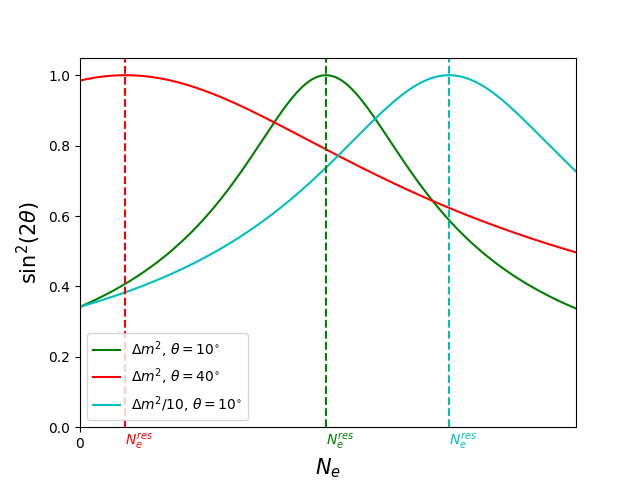
\includegraphics[width=0.5\textwidth,keepaspectratio]{msw_ne.png}
            	\caption[Effet de résonnance \gls{msw}]{\label{fig::amp_matter_vs_Ne}Amplitude de probabilité de changement de saveur de neutrinos se propageant dans la matière (approximation à deux saveur) en fonction de la densité d'électron $N_e$, pour différents angles de mélange dans le vide et différentes différence de masse au carré : il existe une valeur de $N_e$ où cette probabilité est de 1.}
            		%FAIRE un meilleur plot, où l'on voit les tendances à $\pm\infty$, et mettre $\theta_0$ dans le label au lieu de $\theta$.}
            \end{wrapfigure}
            Cette amplitude est représentée en fonction de la densité $N_e$ sur la \autoref{fig::amp_matter_vs_Ne}. On voit qu'elle a un maximum de 1 quand $N_e = N_e^{res}$ et qu'elle tend vers 0 à $\pm\infty$, et ce peu importe l'angle $\theta_0$. Autrement dit, même pour un très petit angle de mélange dans le vide, l'amplitude d'oscillation peut être de 1 si la densité d'électron dans le milieu traversé atteint une valeur de résonance
            \begin{equation}\label{eq::MSW_condition}
                N_e^{res}=\frac{\Delta m^2\cos(2\theta_0)}{2\sqrt{2}G_F E}.%=\numprint{6.56e6}\frac{\Delta m^2(\si{\electronvolt\squared})}{E(\si{\mega\electronvolt})}\cos(2\theta_0)N_A\si{\centi\meter^{-3}}
            \end{equation}
            %où $N_A$ est le nombre d'Avogadro.
            Cet effet, appelé effet \gls{msw}, doit être pris en compte dans les expériences de neutrinos solaires, où la densité décroît depuis le centre du soleil jusqu'à sa surface, dans le cas des neutrinos atmosphériques traversant la Terre, dont le profile de densité peut être vu comme une succession de différentes densités constantes, et dans les expériences à longue ligne de base de réacteur et d'accélérateur, où les électrons traversent la croûte terrestre, dont la densité est en bonne approximation constante.
            
            %Dans le cas des expériences à longue ligne de base de type réacteur ou accélérateur, la densité de matière correspond à celle de la croûte terrestre qui est globalement constante. En revanche, le spectre en énergie des neutrinos incidents peut être large, ce sera le cas notamment pour \gls{dune}. Il est donc plus pratique d'exprimer la condition \eqref{eq::MSW_condition} de la manière suivante : 
            %\begin{equation}
            %    E^{res}=\frac{\Delta m^2\cos(2\theta_0)}{2\sqrt{2}G_F N_e}=\numprint{6.56e6}\frac{\Delta m^2(\si{\electronvolt\squared})}{N_e(N_A\si{\centi\meter^{-3}})}\cos(2\theta_0)(\si{\mega\electronvolt}).
            %\end{equation}
            
            Deux choses sont à noter : 
            \begin{itemize}
            	\item[$\bullet$] Les effets de matière sont sensibles au signes de $\Delta m^2$.
                \item[$\bullet$] Il y a une condition à remplir pour que cette résonance soit possible : il faut que $\frac{\Delta m^2}{2E}\cos(2\theta_0) > 0$ dans le cas des neutrinos et $\frac{\Delta m^2}{2E}\cos(2\theta_0) < 0$ dans le cas des antineutrinos, puisqu'une densité ne peut être négative. Il ne peut donc pas y avoir de résonance à la fois pour les neutrinos \textit{et} pour les antineutrinos. Cet effet induit donc une violation de CP macroscopique dans l'observation des oscillations dans la matière, qui n'a rien à voir avec la phase de violation de CP de la matrice PMNS, et qu'il convient de modéliser précisément pour toute tentative de mesure de $\delta_{CP}$.
                \item[$\bullet$] Si l'angle de mélange dans le vide est strictement nul, il ne peut pas y avoir de résonance. En effet, dans ce cas, l'équation \eqref{eq::tan2theta} donne $\tan(2\theta)=0$ et donc $\theta=\frac{\pi}{2}$, rendant les états propres de saveurs orthogonaux et donc non-mélangeables.
                \item[$\bullet$] Si $N_e$ est variable le long du parcours des neutrinos, ce qui est le cas des neutrinos solaires ou des neutrinos passant par le centre de la Terre, la résonance est atteinte si au moins une région à un $N_e$ satisfaisant \eqref{eq::MSW_condition}. Ces cas ne correspondant pas aux expériences de neutrinos d'accélérateurs à longue ligne de base, aussi nous ne les détaillons pas. Un traitement de ces cas peut être trouvé ici \cite{Akhmedov2000}.
                \item[$\bullet$] Si les neutrinos ont un spectre en énergie relativement large, la résonance ne peut être atteinte que par une certaine partie du spectre seulement.
                \item[$\bullet$] En pratique, pour une source de neutrinos donnée, l'effet \gls{msw} se manifestera pour deux régions d'énergie, correspondant à la condition \eqref{eq::MSW_condition} satisfaite avec $\Delta m^2_{21}$ ou $\Delta m^2_{31}\simeq\Delta m^2_{32}$.
            \end{itemize}
                
            
        \subsection{Le cas à trois saveurs}\label{sec::3flavor_matter}
            Le calcul des effets de matière à trois saveurs suit la même logique que le cas à deux saveurs : il faut définir un nouvel Hamiltonien comme dans l'équation \eqref{eq::hamiltonian_matter_2flavor} et le diagonaliser pour trouver les nouveaux vecteurs et valeurs propres et la matrice de mélange dans la matière. Les calculs sont effectués en détails par Freund \cite{Freund2001}, aussi ne sont-ils pas refaits ici. Un point est à souligner : le calcul des vecteurs et valeurs propres s'effectue par développement en série, autour de $\alpha=\Delta m^2_{21}/\Delta m^2_{31}$. Il en ressort deux résultats possibles, suivant que le paramètre $\hat{A}=\frac{2V_{CC}E}{\Delta m^2_{31}}$ est petit ou non, qui correspondent aux deux résonances \gls{msw} possibles, à savoir la résonance solaire quand $\hat{A}=\alpha\simeq\numprint{0.03}$ et la résonance atmosphérique quand $\hat{A}=\cos(2\theta_{13})\simeq \numprint{0.95}$. Le cas qui nous intéresse est $|\hat{A}|>\alpha$c, qui est approprié pour des énergies de neutrinos de l'ordre du \si{\giga\electronvolt} et des densités de matière proche de celle de la croûte terrestre.
            
            En prenant en compte les effets de matière, la probabilité $P(\nu_{\mu}\to\nu_e)$ développée dans l'équation \eqref{eq::dvpt_3flavor_accelerator}, qui est d'intérêt pour les expériences de neutrinos d'accélérateurs, devient alors\cite{Giganti2017}
            \begin{equation}\label{eq::proba_matter_3flavors}
	            \begin{split}
	            P(\nu_{\mu}\to\nu_e) & \simeq  \sin^2(\theta_{23})\frac{\sin^2(2\theta_{13})}{(A-1)^2}\sin^2\left[(A-1)\Delta_{31}\right]
	            + \alpha^2\cos^2(\theta_{23})\frac{\sin^2(2\theta_{12})}{A^2}\sin^2\left(A\Delta_{31}\right) \\ 
	            & + \alpha\frac{\cos(\theta_{13})\sin(2\theta_{12})\sin(2\theta_{13})\sin(2\theta_{23})\cos(\delta_{CP})}{A(1-A)}\cos\left(\Delta_{31}\right)\sin\left(A\Delta_{31}\right)\sin\left[(1-A)\Delta_{31}\right] \\
	            & - \alpha\frac{\cos(\theta_{13})\sin(2\theta_{12})\sin(2\theta_{13})\sin(2\theta_{23})\sin(\delta_{CP})}{A(1-A)}\sin\left(\Delta_{31}\right)\sin\left(A\Delta_{31}\right)\sin\left[(1-A)\Delta_{31}\right]
	            \end{split}
            \end{equation}
            où $\Delta_{31}=\Delta m^2_{31}\frac{L}{4E}$, $\alpha=\Delta m^2_{21}/\Delta m^2_{31}\simeq 0.03$  et $A=2VE/\Delta m^2_{31}=2\sqrt{2}G_F N_eE/\Delta m^2_{31}$. Le premier terme, où $\alpha$ n'apparaît pas, est dominé par $\Delta m^2_{31}$. Le second terme, fortement supprimé par $\alpha^2$, est dominé par $\Delta m^2_{21}$. Pour avoir la probabilité $P(\overline{\nu}_{\mu}\to\overline{\nu}_e)$, il faut alors inverser le signe de $\delta_{CP}$ et de $A$. Changer le signe de $\delta_{CP}$ change le signe du terme impair en $\delta_{CP}$, alors que changer le signe de $A$ aura une influence sur tous les termes sauf le second. Les effets de matière et la phase de violation de CP ont donc un impact différent sur la probabilité d'oscillation, mais si les effets de matière sont trop importants, il peuvent nuire à la mesure de $\delta_{CP}$.

            %Dans le cas à trois saveurs, l'équation \eqref{eq::evolution_matter_2flavor} devient, en prenant en compte le potentiel $V_{CC}$ :
            %\begin{equation}\label{eq::evolution_matter_3flavor}
             %   i\frac{d}{dt}\left(\begin{matrix}\nu_e \\ \nu_{\mu} \\ \nu_{\tau}\end{matrix}\right) = \left [ \frac{1}{2E}U\underbrace{\left(\begin{matrix} m_1^2 & 0 & 0 \\ 0 & m_2^2 & 0 \\
              %  0 & 0 & m_3^2\end{matrix}\right)}_{M^2}U^{\dagger} + \left(\begin{matrix}V_{CC} & 0 & 0 \\ 0 & 0 & 0 \\ 0 & 0 & 0\end{matrix}\right)\right]\left(\begin{matrix}\nu_e \\ \nu_{\mu} \\ \nu_{\tau}\end{matrix}\right)
            %\end{equation}
            
            %\subsubsection{Justification de l'approximation à deux saveurs}
            %Si l'approximation \eqref{eq::approx_21_0} est valide, il est utile d'effectuer la transformation 
            %\begin{equation}
             %   M^2\to \widetilde{M}^2 = M^2-m_1^2\mathbb{I}=\left(\begin{matrix} 0 & 0 & 0 \\ 0  & \Delta m^2_{21} & 0 \\ 0 & 0 & \Delta m^2_{31}\end{matrix}\right) \simeq \left(\begin{matrix} 0 & 0 & 0 \\ 0  & 0 & 0 \\ 0 & 0 & \Delta m^2_{31}\end{matrix}\right)
            %\end{equation}
            %où le terme $m_1^2\mathbb{I}$ peut être absorbé par rephasage dans l'équation \eqref{eq::evolution_matter_3flavor}. Cette matrice commute avec $u_{12}$. En notant $V=\text{diag}(V_{CC},0,0)$, qui commute avec $u_{23}$, et $ \widetilde{\nu} = u_{23}\left(\nu_e, \nu_{\mu}, \nu_{\tau}\right)^T$, on obtient donc
            %\begin{eqnarray}
             %   & i\frac{d}{dt}\widetilde{\nu} = \left(\frac{1}{2E}u_{13}\widetilde{M}^2u^{\dagger}_{13} + V\right)\widetilde{\nu} \\ 
              %  \Rightarrow & i\frac{d}{dt}\left(\begin{matrix}\widetilde{\nu_a} \\ \widetilde{\nu_b} \\ \widetilde{\nu_c}\end{matrix}\right) = \left(\begin{matrix}  \frac{\Delta m^2_{31}}{2E}s^2_{13}+V_{CC} & 0 & \frac{\Delta m^2_{31}}{2E}s_{13}c_{13} \\ 0  & 0 & 0 \\ \frac{\Delta m^2_{31}}{2E}s_{13}c_{13} & 0 & \frac{\Delta m^2_{31}}{2E}c^2_{13} \end{matrix}\right)\left(\begin{matrix}\widetilde{\nu_a} \\ \widetilde{\nu_b} \\ \widetilde{\nu_b}\end{matrix}\right)
            %\end{eqnarray}
            %où $\widetilde{\nu_a} = \nu_e$ et $\widetilde{\nu_c} = s_{23}\nu_{\mu} + c_{23}\nu_{\tau}$.
            %Le problème se réduit donc à un problème d'oscillation à deux saveurs entre $\widetilde{\nu_a}$ et $\widetilde{\nu_b}$ où, après un dernier rephasage, on peut écrire
            %\begin{equation}
            %    i\frac{d}{dt}\left(\begin{matrix}\widetilde{\nu_a} \\ \widetilde{\nu_b}\end{matrix}\right) = \left(\begin{matrix} -\frac{\Delta m^2_{31}}{4E}\cos(2\theta_{13}) + \frac{V_{CC}}{2} & \frac{\Delta m^2_{31}}{4E}\sin(2\theta_{13}) \\ 
           %     \frac{\Delta m^2_{31}}{4E}\sin(2\theta_{13}) & \frac{\Delta m^2_{31}}{4E}\cos(2\theta_{13}) - \frac{V_{CC}}{2}\end{matrix}\right)\left(\begin{matrix}\widetilde{\nu_a} \\ \widetilde{\nu_b}\end{matrix}\right).
           % \end{equation}
            %\subsubsection{Approximation pour les expériences de neutrinos d'accélérateurs à longue ligne de base}

    \section{État de l'art}
    
	    \subsection{Les connaissances actuelles}
	   
		   \begin{table}[!h]
		   	\centering
		   	\begin{tabular*}{\textwidth}{@{\extracolsep{\fill}}|r||lclcl|} 
		   		\hline
		   		\textbf{Type d'expérience}            & $\mathbf{L}$ \textbf{[m]}  & & $\mathbf{E}$ \textbf{[MeV]}   & & $\mathbf{\Delta m^2}$ \textbf{[eV$^2$]}   \\ 
		   		\hline
		   		\hline
		   		Solaire                       & \numprint{e11}               & &1                          & &\numprint{e-11}             \\ 
		   		Atmosphérique                 & \numprint{e4} -- \numprint{e7}    & &\numprint{e2} -- \numprint{e5}       & &\numprint{e-1} -- \numprint{e-4} \\ 
		   		Réacteur                     & \numprint{e2} -- \numprint{e6}    & &1                          & &\numprint{e-2} -- \numprint{e-3} \\ 
		   		Accélérateur                 & \numprint{e2}                & &\numprint{e3} -- \numprint{e4}       & &$\gtrsim \numprint{0.1}$          \\ 
		   		Accélérateur à longue ligne de base   & \numprint{e5} -- \numprint{e6}    & &\numprint{e4}                   & &\numprint{e-2} -- \numprint{e-3} \\
		   		\hline
		   	\end{tabular*}
		   	\caption[Valeurs de $L$ et $E$ pour différents types d'expériences.]{Valeurs de $L$ et $E$ pour différents types d'expériences et valeur mesurables de $\Delta m^2$.}
		   	\label{tab::carac-experiments}
		   \end{table} 
	   
		    Il existe plusieurs sources capables de nous donner des renseignements sur les oscillations des neutrinos. La nature des informations accessibles dépend principalement des énergies $E$ et des lignes de base $L$. Le \autoref{tab::carac-experiments} présente ces différentes grandeurs pour les types d'expériences présentés ci-dessous, et précise les valeurs de $\Delta m^2$ mesurables.
		    
		    	\begin{figure}[htpb]
		    		\centering
		    		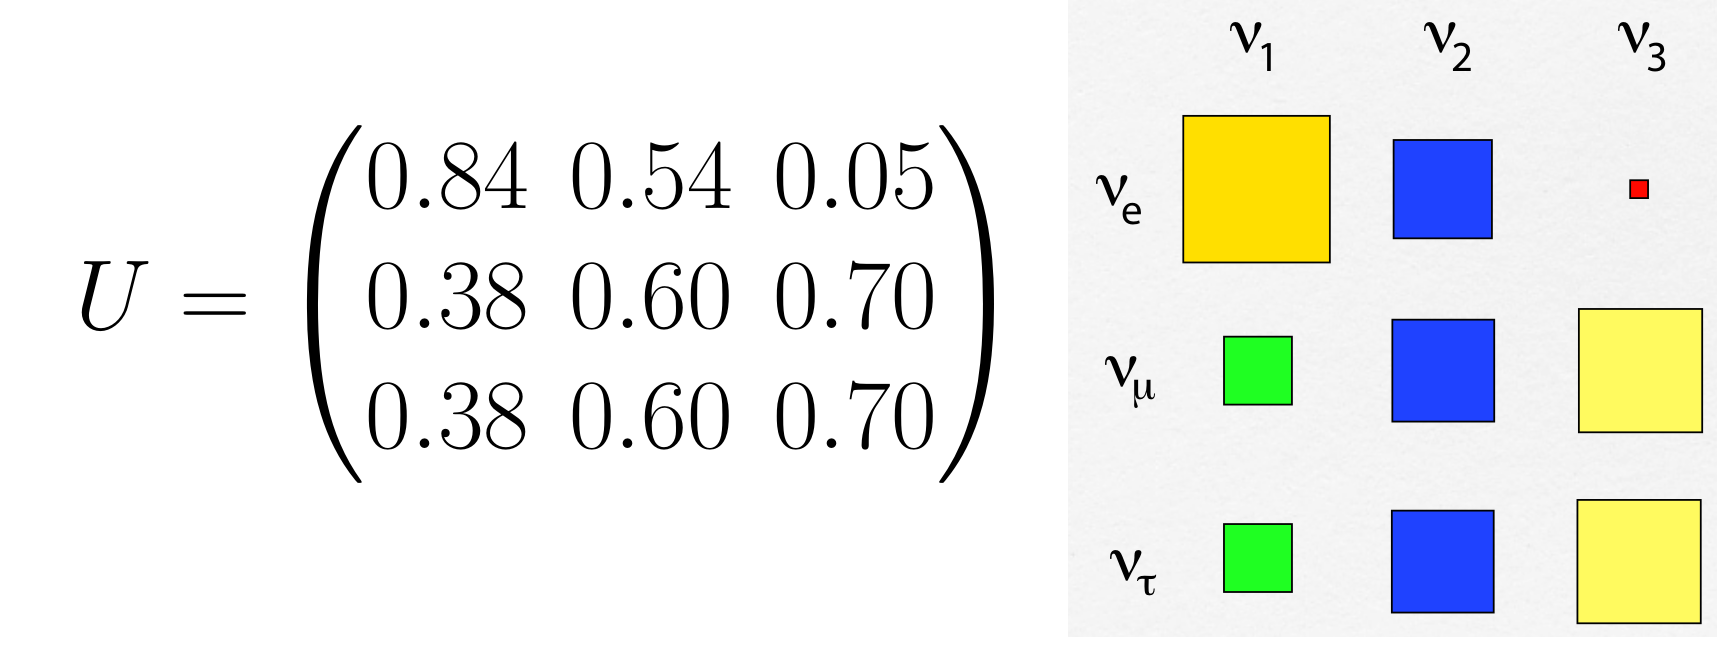
\includegraphics[width=.8\textwidth,keepaspectratio]{pmns.png}
		    		\caption[La matrice PMNS.]{Coefficients de la matrice PMNS. Image tirée de \cite{King2015}. Contrairement à la matrice CKM de mélange des quarks, qui est presque diagonale, le mélange des saveurs est très important dans le secteur leptonique.}
		    		\label{fig::pmns}
		    	\end{figure}
		    
		     Il y a des sources naturelles :
		    \begin{itemize}
		    	\item[$\bullet$] Les neutrinos solaires, issus des réactions de fusion nucléaire au coeur du soleil, sont des $\nu_e$ à leur création mais un certain nombre auront oscillé vers une autre saveur en quittant le soleil dû aux effets de matière décrits en \autoref{sec::matter_effect}. Plusieurs réactions entrent en jeu, chacune produisant des neutrinos d'énergies différentes et à des flux différents. %La figure \autoref{fig::solar_flux} montre les prédictions de ces flux par le Modèle Solaire Standard\cite{Bahcall2005}. 
		    	Ces neutrinos sont caractérisés par une énergie assez basse (de l'ordre du \si{\mega\electronvolt}) mais une ligne de base très longue, à savoir la distance Terre-Soleil.
		    	\item[$\bullet$] Les neutrinos atmosphériques, issus de la désintégrations de mésons et muons produits par les interactions des rayons cosmiques avec l'atmosphère, peuvent être à leur création des $\nu_{\mu}$, $\overline{\nu}_{\mu}$, $\nu_e$ et $\overline{\nu}_e$. Ils ont une énergie comprise entre 1 et $\SI{e5}{\giga\electronvolt}$ et une ligne de base allant de \SI{15}{\kilo\meter} pour les neutrinos arrivant du haut à \SI{12000}{\kilo\meter} pour ceux arrivant de l'autre côté du globe. Ces neutrinos subissent les effets de matière en traversant la Terre. Il est donc possible, pour une même source de neutrinos, de couvrir un large spectre de $L/E$. %La figure \autoref{fig::atm_flux} montre le spectre en énergie de ces neutrinos.
		    \end{itemize}
		    
		    et des sources artificielles:
		    \begin{itemize}
		    	\item[$\bullet$] Les neutrinos de réacteurs, issus des réactions de fissions au cœur des réacteurs nucléaires, sont des $\overline{\nu}_e$, avec un spectre en énergie allant de 1 à \SI{10}{\mega\electronvolt}.
		    	% montré en figure \autoref{fig::reactor_flux}. 
		    	L'avantage de ces expériences est qu'il est possible, dans une certaine limite, de choisir la ligne de base afin d'optimiser une oscillation autour d'un $\Delta m^2$ en fixant une valeur de $1.27\Delta m^2\frac{L}{E}$ proche de $\pi/2+n\pi$ afin de maximiser le terme en $\sin^2(1.27\Delta m^2\frac{L}{E})$.
		    	\item[$\bullet$] Les neutrinos d'accélérateurs, issus de faisceaux produit par l'homme, sont des $\nu_{\mu}$ (voir \autoref{sec::faisceau}). L'énergie est ajustable et le spectre peut être choisi de manière à être très piqué autour d'une valeur, comme dans l'expérience T2K, en plaçant la détecteur légèrement hors de l'axe du faisceau\cite{McDonald2001}, ou large, afin de couvrir plusieurs pics de $1.27\Delta m^2\frac{L}{E}=\pi/2+n\pi$. Ce sera le cas pour la future expérience \gls{dune}. De plus, la ligne de base est également ajustable.
		    \end{itemize}
		    Dans les deux cas de sources artificielles, si la ligne de base est grande, les neutrinos traverseront nécessairement la croûte terrestre et des effets de matière entreront alors en jeu.
		    
		    \begin{table}[!t]
		    	\centering
		    	\begin{tabular*}{\textwidth}{@{\extracolsep{\fill}}|r|cc|}
		    		\hline
		    		\textbf{Paramètre} & \textbf{meilleur ajustement} & \textbf{3}$\mathbf{\sigma}$  \\
		    		\hline
		    		\hline
		    		$\Delta m^2_{21}~[\SI{e-5}{\electronvolt\squared}]$ & \numprint{7.37}   & \numprint{6.93}--\numprint{7.96}\\
		    		$|\Delta m^2_{31}|~[\SI{e-3}{\electronvolt\squared}]$ & \numprint{2.56}   & \numprint{2.45}--\numprint{2.69} \\
		    		$\sin^2\theta_{12}$ & \numprint{0.297}   & \numprint{0.250}--\numprint{0.354}\\
		    		$\sin^2\theta_{23}$, $\Delta m^2_{31(23)}>0$ & \numprint{0.425}   & \numprint{0.381}--\numprint{0.615}\\
		    		$\sin^2\theta_{23}$, $\Delta m^2_{31(23)}<0$ & \numprint{0.589}   & \numprint{0.384}--\numprint{0.636}\\
		    		$\sin^2\theta_{13}$, $\Delta m^2_{31(23)}>0$ & \numprint{0.0215}   & \numprint{0.0190}--\numprint{0.0240}\\
		    		$\sin^2\theta_{13}$, $\Delta m^2_{31(23)}<0$ & \numprint{0.0216}   & \numprint{0.0190}--\numprint{0.0242}\\
		    		$\delta_{CP}/\pi$, $\Delta m^2_{31(23)}>0$ & \numprint{1.38} & $2\sigma$ :\numprint{1.0}--\numprint{1.9} \\
					\hline
		    	\end{tabular*}
		    	\caption[Meilleurs ajustements des mesures des paramètres des oscillations des neutrinos.]{\label{tab::pmns_values}Meilleurs ajustements des mesures des paramètres des oscillations, tiré la version de 2018 du PDG\cite{pdg2018}. Les incertitudes sont données à $3\sigma$, sauf pour $\delta_{CP}$ où elles sont données à $2\sigma$.}
		    \end{table}
		    
		    Les premières mesures de neutrinos atmosphériques, faites par Super-Kamiokande\cite{Fukuda1998}, ont montré que le flux des neutrinos électroniques ne présentait pas particulièrement d'excès ni de déficit, contrairement aux neutrinos muoniques. La probabilité de survie de ces derniers, en utilisant les approximations \eqref{eq::approx_21_0} et \eqref{eq::approx_13_eq_0}, s'écrit
		    \begin{equation}
		    P(\nu_{\mu}\to\nu_{\mu}) = 1 - \sin^2(2\theta_{23})\sin^2\left(\Delta m^2_{31}\frac{L}{4E}\right).
		    \end{equation}
		    De ce fait, la matrice $u_{23}$ est appelée matrice du "secteur atmosphérique". Ce secteur est également accessible grâce aux expériences de neutrinos d'accélérateurs à longue ligne de base, décrites plus en détail au chapitre suivant. Les principales expériences de neutrinos d'accélérateurs ayant fourni des résultats dans le secteur atmosphérique sont K2K\cite{Collaboration2006a}, T2K\cite{Abe2018}, NO$\nu$A\cite{Adamson2016} et MINOS\cite{Collaboration2014}. La mesure la plus précise à ce jour, issue d'un ajustement global des données actuelles, donne à $3\sigma$ $\sin^2(\theta_{23})=\numprint{0.425}^{+\numprint{0.19}}_{-\numprint{0.044}}$\cite{pdg2018} si la hiérarchie de masse est normale (voir \autoref{sec::hierarchy}), $\sin^2(\theta_{23})=0.589^{+0.047}_{-0.205}$ si elle est inversée. Ceci correspond à $\theta_{23}\simeq\SI{41}{\degree}$ si la hiérarchie est normale, et $\theta_{23}\simeq\SI{50}{\degree}$ si elle est inversée.
		    
		    Les approximations \eqref{eq::approx_31_eq_32} et \eqref{eq::approx_13_eq_0}, donnant la probabilité de survie des neutrinos électroniques venus du soleil \eqref{eq::solar_oscillation}, justifie que la matrice $u_{12}$ soit appelée matrice du "secteur solaire". Elle fut la première a être étudiée, surtout par Homesteak\cite{Lande1990}, SAGE\cite{Collaboration2009}, Gallex/GNO\cite{Hampel1999}, et plus tard par SNO\cite{Aharmim2013},  Kamiokande-II\cite{Hirata1992}, Super-Kamiokande\cite{Abe2018} et Borexino\cite{Collaboration2013}. KamLand\cite{Collaboration2004}, une expérience de neutrino de réacteur, a également fournit des informations sur le secteur solaire. La mesure la plus précise à ce jour, issue d'un ajustement global des données actuelles donne $\sin^2(\theta_{12})=\numprint{0.297}^{+\numprint{0.057}}_{-\numprint{0.047}}$\cite{pdg2018}, correspondant à $\theta_{12}\simeq\SI{33}{\degree}$, où les incertitudes correspondent à $3\sigma$.
		    
		    Les approximations \eqref{eq::approx_21_0} et \eqref{eq::approx_13_eq_0} donnent $P(\overline{\nu}_e\to\overline{\nu}_e) = 1-\sin^2(2\theta_{13})\sin^2\left(\Delta m^2_{31}\frac{L}{4E}\right)$ comme probabilité de survie des antineutrinos électroniques, approximations valables pour les expériences de neutrinos de réacteurs. Ceci justifie que la matrice $u_{13}$ soit appelée matrice du "secteur réacteur". La petite valeur de $\theta_{13}$ (inférieur à $\SI{10}{\degree}$) le rend plus difficilement mesurable. Les mesures des termes solaires et atmosphériques ont permis de déterminer qu'avec une ligne de base d'environ \SI{2}{\kilo\meter}, un détecteur proche d'un réacteur pouvait mesurer $\theta_{13}$, ce qui a été fait par Double Chooz\cite{Crespo-Anadon2014}, Reno\cite{Collaboration2010} et Daya Bay\cite{An2014}. Les expériences de neutrinos d'accélérateur à longue ligne de base K2K\cite{Collaboration2006a}, MINOS\cite{Collaboration2014} et T2K\cite{Abe2018} ont également fourni des résultats concernant $\theta_{13}$. La mesure la plus précise à ce jour, issue d'un ajustement global des données actuelles donne à $3\sigma$ $\sin^2(\theta_{13})=\numprint{0.0215}^{+\numprint{0.025}}_{-\numprint{0.025}}$\cite{pdg2018} si la hiérarchie de masse est normale (voir \autoref{sec::hierarchy}), $\sin^2(\theta_{13})=\numprint{0.0216}^{+\numprint{0.026}}_{-\numprint{0.026}}$ si elle est inversée. Ceci correspond à $\theta_{13}\simeq\SI{8.44}{\degree}$.
		    
		    \subsection{Ce qu'il reste à découvrir}
		    
			    La découverte des oscillations des neutrinos soulève beaucoup de questions, comme : pourquoi sont-ils aussi légers? Quelle est l'origine de leurs masses? Pourquoi deux différences de masse au carré sont si proches? Les neutrinos sont-ils de Dirac ou de Majorana? La matrice PMNS à 3 dimensions est-elle unitaire? Les neutrinos violent-ils la symétrie CP? Quelle est la hiérarchie de leur masse? Parmi toutes ces question, l'expérience \gls{dune} traitera essentiellement les deux dernières, détaillées maintenant.
		    
%		        \subsubsection{La matrice PMNS à plus de trois dimensions}
%		        
%	            Il n'est pas possible de généraliser brutalement l'expression \eqref{eq::pmns} à $n>3$ dimensions sans perdre en sens physique. En effet, $n$ dimensions implique $n$ types de neutrinos, et $n$ leptons chargés, mais ces derniers sont au nombre de 3.
%	            
%	            Que se passe-t-il si il existe plus de 3 neutrinos? Tout d'abord, ils ne peuvent pas interagir via l'interaction faible, comme nous l'avons mentionné plus haut. Ils ne se couplent donc pas aux leptons chargés. Même dans le cas où ces neutrinos sont de Dirac, nous ne pourrons plus éliminer autant de phases qu'avant. En effet, même si il existe $n$ neutrinos, il n'existe quand même que 3 leptons chargés, et donc il n'y a toujours que 5 phases qui pourront s'annuler, laissant dans la matrice $U$ un total de $2n-5$ phases similaires à $\delta_{CP}$. Si les neutrinos sont de Majorana, il y aura alors $n-1$ phases de Majorana.
%	            
%	            Si il existe plus de 3 saveurs de neutrinos pouvant se mélanger, alors la matrice PMNS ne devrait pas être unitaire. C'est en testant cette unitarité que l'on peut déterminer la dimension de la matrice. Un article de 2018\cite{Qian2013} décrit comment réaliser un tel test, qui requière plus de données que ce que l'on a actuellement pour donner un résultat précis. Pour le moment, les données sont compatibles avec une matrice PMNS à trois dimensions unitaire, et pose une limite sur les couplages avec un possible quatrième neutrino.
	            
	        
		        \subsubsection{La hiérarchie de masse}\label{sec::hierarchy}
		        
		        \begin{wrapfigure}{R}{0.5\textwidth}
		        	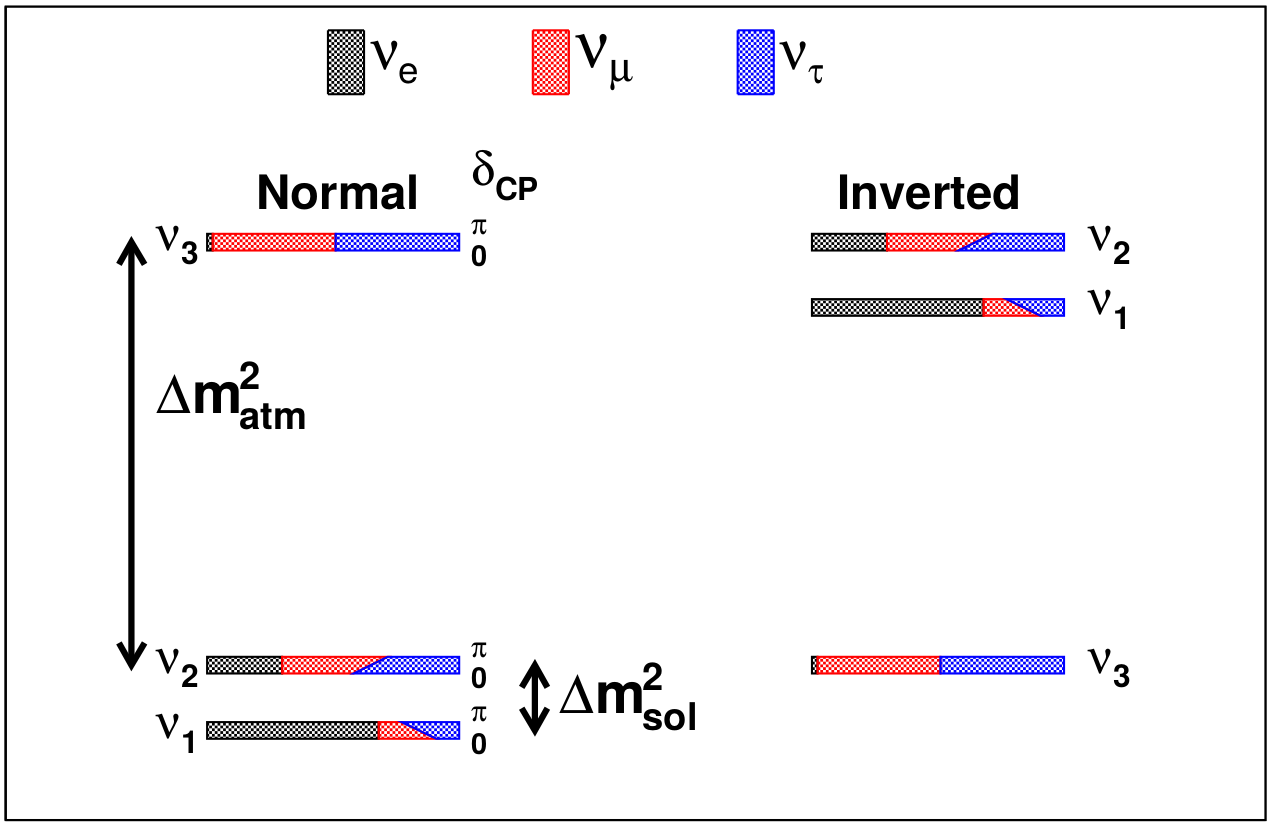
\includegraphics[width=0.5\textwidth,keepaspectratio]{mass_hierarchy.png}
		        	\caption[Les deux hiérarchies de masse possibles]{\label{fig::mass_hierarchy}Les deux hiérarchies de masse possibles et leurs composition en états de saveurs en fonction de la valeur de $\delta_{CP}$. Tiré de \cite{Qian2015}.}
		        \end{wrapfigure}
	            Les phénomènes observables liés aux oscillations des neutrinos font intervenir des termes de différence de masse au carré. En mesurer deux permet de calculer la troisième sans ambiguïtés. Les données expérimentales des expériences d'oscillations des neutrinos solaires et atmosphériques ont montré qu'il existe une certaine hiérarchie dans les masses des neutrinos. En effet, elles sont telles que
	            \begin{equation}\label{eq::mass_hierarchy}
	            	|\Delta m^2_{21}| <<|\Delta m^2_{31}| \simeq |\Delta m^2_{32}| 
	            \end{equation}
	            Ceci peut correspondre à quatre ordres différents pour les 3 masses $m_1$, $m_2$ et $m_3$. Parmi ces 4, deux couples sont équivalents\cite{pdg2018}, et la convention utilisée le plus souvent est celle posant $\Delta m^2_{21} > 0$. Il reste alors deux possibilités. La \autoref{fig::mass_hierarchy} montre ces deux possibilités ainsi que leur composantes respective en $\nu_e$, $\nu_{\mu}$ et $\nu_{\tau}$, pour des valeurs de $\delta_{CP}$ allant de 0 à $\pi$\cite{Qian2015}. La convention est d'appeler le cas $m_1 < m_2 < m_3$ hiérarchie normale et le cas $m_3 < m_1 < m_2$ hiérarchie inversée.
	            
	            Les premières générations d'expériences d'oscillation de neutrinos, où les effets de matières étaient absents\footnote{Sauf dans le cas des neutrinos solaires, mais la convention avait déjà posé $\Delta m^2_{21} > 0$, qui est la seule accessible par ces expériences.}, utilisaient l'approximation à deux saveurs \eqref{eq::two_flavors}, n'étant pas assez précises pour déceler des effets à trois saveurs. Le terme d'oscillation étant en $\sin^2$, il n'est pas sensible au signe de $\Delta m^2$, aussi nous ne savons toujours pas laquelle des deux hiérarchies est la bonne. Il est important de lever cette inconnue, la hiérarchie de masse est liée  un certain nombre de théories concernant la grande unification des forces fondamentales, l'origine de l'univers, ou même la production d'isotopes au sein des étoiles\cite{KH-website}.
	            
	            Une des manières de déterminer la hiérarchie de masse est d'utiliser les effets de matière. En effet, la résonance \gls{msw} dépend directement de $\Delta m^2$, comme le montre l'approximation à deux saveur \eqref{eq::MSW_condition} : si $\sin(2\theta_{13})\Delta m^2_{31} > 0$, alors on devrait pouvoir observer cette résonance en ajustant correctement l'énergie des neutrinos. Les résultats présentés dans le \autoref{tab::pmns_values} montre que $\sin(2\theta_{13}) > 0$, et donc une observation de cette résonance avec des neutrinos montrerait que la hiérarchie est normale. À l'inverse, une suppression due aux effets de matière montrerait que la hiérarchie est inversée (inversement si l'expérience est faite avec des antineutrinos). Ceci peut être fait avec des antineutrinos électroniques de réacteur, comme dans la future expérience JUNO\cite{Yang2015}, où l'on mesure la probabilité de survie de ces derniers, ou avec des (anti)neutrinos muoniques de faisceau, où l'on s'intéresse à la probabilité d'oscillation en (anti)neutrinos électroniques. Dans les deux cas, la ligne de base doit être assez importante pour donner lieu à des effets de matière conséquents.
	            
	            Dans le cadre de l'expérience \gls{dune}, la probabilité \eqref{eq::proba_matter_3flavors} et son analogue avec des antineutrinos seront mesurées et comparées à la prédiction. Les résultats attendus ainsi que les sensibilités sont présentés en \autoref{sec::dune_pheno}. 
	            
	        \subsubsection{La violation de CP et l'asymétrie matière / anti-matière}\label{sec::CP_violation}
	            La matrice \gls{pmns} a la même structure et les même propriétés que la matrice CKM qui décrit le mélange de saveur des quarks, puisque ces deux matrices décrivent le même phénomène. Dans le formalisme de la matrice CKM, C.~Jarlskog a montré que la transition d'une saveur à l'autre peut ne pas être la même entre particule et antiparticule si une certaine grandeur, appelé invariant de Jarlskog, est non nulle\cite{Jarlskog1985}. Dans le formalisme de la matrice \gls{pmns}, cette grandeur est
	            \begin{equation}
	                J_{CP}^{PMNS}=\frac{1}{8}\sin(2\theta_{12})\sin(2\theta_{13})\sin(2\theta_{23})\cos(\theta_{13})\sin(\delta_{CP}).
	            \end{equation}
	            Cette grandeur est appelé invariant car elle ne dépend pas de la paramétrisation choisie pour la phase de violation CP. On peut noter que si un seul des angles est nul, alors $J_{CP}^{PMNS}$ est nulle et les neutrinos et antineutrinos oscillent de la même manière (en absence d'effets de matière). Mais les mesures actuelles (voir \autoref{tab::pmns_values}) montrent qu'aucun des trois angles n'est nul. Dans ce cas, seule une valeur de $0$ ou $\pi$ pour $\delta_{CP}$ conserverait la symétrie CP. Les mesures les plus récentes de T2K excluent ces valeurs a $2\sigma$\cite{Abe2018} si la hiérarchie de masse est normale, mais ne sont pas assez précises pour donner une valeur exacte de $\delta_{CP}$. Or, cette valeur joue un rôle fondamental dans la question "pourquoi y a-t-il quelque chose plutôt que rien?", comme nous l'avons mentionné en \autoref{sec::CP}.
	            
	            Un papier récent\cite{Buccella2018}  a montré que, sous certaines contraintes, une valeur de $\delta_{CP}$ comprise entre $-\numprint{0.9}\pi$ et $-\numprint{0.75}\pi$ serait suffisante pour expliquer cette asymétrie. Pour ce faire, il est nécessaire d'atteindre des précisions où les oscillations à trois saveurs sont importantes. En effet, la probabilité de transition à deux saveurs \eqref{eq::two_flavors} ne fait pas intervenir $\delta_{CP}$, contrairement à la probabilité à trois saveurs \eqref{eq::proba_oscillation}. Pour les expériences à longue ligne de base, il est en plus nécessaire d'avoir une région du signal où l'effet de violation de CP dû à $\delta_{CP}$ est séparable de l'effet due aux effets de matière. En effet,  \gls{dune} mesurera la probabilité \eqref{eq::proba_matter_3flavors} et son analogue avec des antineutrinos. Les mesures seront comparées à la prédiction, les résultats attendus ainsi que les sensibilités sont présentés en \autoref{sec::dune_pheno}.
        
        \printbibliography
\chapter{L'expérience \texorpdfstring{DU$\nu$E}{DUNE} et son projet de R\&D~: \texorpdfstring{protoDU$\nu$E}{protoDUNE}}
    \chapterprecishere{
        ``Potentielle citation sans aucun rapport avec le sujet"\par\raggedleft--- \textup{Personne inconnue}, contexte à déterminer
    }
    
    Ce chapitre commence par introduire les principales expériences d'oscillation de neutrinos d'accélérateurs à long ligne de base, dont \gls{dune} fait parti, en expliquant leurs points forts et leurs points faibles. Ensuite, une section est dédiée à l'expérience \gls{dune} elle même, puis une autre section est dédiée au projet \gls{wa105} faisant parti des expériences de prototypage de \gls{dune}.
        
    \section{DU$\nu$E, une expériences d'oscillation de neutrinos d'accélérateurs à long ligne de base}
    
        \gls{dune} est une expérience d'oscillation des neutrinos à longue ligne de base, qui enverra un faisceau de neutrino depuis le Fermilab (Illinois) vers l'installation de recherche souterraine de Sanford (Dakota du sud)(voir \autoref{fig::dune}). Les neutrinos, créé par un accélérateur de proton, parcourront $\SI{1300}{\kilo\meter}$ à travers la croûte terrestre avant d'être détectés par quatre \glspl{tpc}, chacune remplies de $\SI{10}{\kilo\tonne}$ d'argon. Ses objectifs sont multiples, mais les principaux sont la mesure de la phase de violation CP et la détermination de la hiérarchie de masse, en mesurant la probabilité d'apparition $P(\nu_{\mu}\to\nu_e)$ de neutrinos électroniques dans un faisceau initialement constitué de neutrinos muoniques.
        
        Les expériences à longue ligne de base sont caractérisées par le fait de chercher à atteindre un maximum de probabilité d'oscillation (voir \autoref{sec::oscillations}) en plaçant un détecteur loin de la source et en cherchant à détecter des neutrinos d'énergies correspondantes à ce maximum. Dans ces expériences, les neutrinos peuvent être issus de réacteurs nucléaire (comme dans l'expérience JUNO\cite{juno}), du soleil (expérience SNO\cite{sno}), de réactions de rayons cosmiques dans l'atmosphère (expérience Super Kamiokande\cite{skk_atm}), de supernovae (expérience Super Kamiokande\cite{skk_atm}) ou de faisceaux créés par l'homme, comme \gls{dune}.
        
        \subsection{Qu'est ce qu'une expérience d'oscillation de neutrinos d'accélérateurs à longue ligne de base?}
            
            Comme il est discuté en \autoref{sec::oscillations}, la probabilité qu'a un neutrino de changer de saveur oscille avec le ratio $L/E$, où $L$ est la distance entre le point d'origine du neutrino et l'endroit où il est détecté (ligne de base), et $E$ est l'énergie de ce neutrino. Ce phénomène étant oscillant, il existe des ratios $L/E$ privilégiés pour la détection des changements de saveur, où la probabilité de changement est localement maximale. La \autoref{fig::numu-oscillation} montre la probabilité qu'a un neutrino initialement muonique, comme ce sera le cas pour \gls{dune}, de se changer en une autre saveur, en fonction de $L/E$. Les expériences cherchant à détecter les oscillations des neutrinos vont chercher à se placer à une ligne de base tel que $L/E$ correspond à un de ces maxima. L'expérience \gls{dune} sera capable de couvrir deux de ces maxima ce qui permettra à la fois de déterminer la hiérarchie de masse et de mesurer la phase de violation CP (voir \autoref{sec::dune}). 
            
            Les expériences d'oscillation de neutrinos d'accélérateurs à longue ligne de base cherchent à mesurer la probabilité d'oscillation $P(\nu_{\mu}\to \nu_e)$ en fonction de l'énergie du neutrino incident en détectant les produits de réaction des neutrinos d'un faisceau initialement composé uniquement de neutrinos muoniques. Le détecteur doit donc être capable de différencier une réaction de neutrino muonique d'une réaction de neutrino électronique, ainsi que de mesurer précisément l'énergie mise en jeu dans ces réactions. Le faisceau de neutrino, dont le principe est décrit en \autoref{sec::faisceau}, va d'abord traverser un détecteur placer proche de la source, typiquement à quelques centaines de mètres, quand la probabilité d'oscillation est encore nulle. Les caractéristiques importantes du faisceau y sont analysées, comme le flux et le spectre en énergie. Le faisceau parcours ensuite une grande distance à travers la croûte terrestre jusqu'au détecteur lointain. 
            
            La possibilité de comparer les observations avant et après oscillation d'une même source de neutrinos est une plus-value des expériences à longue ligne de base utilisant des faisceaux ou des réacteurs. Une plus-value du faisceau est son ajustabilité en flux et en énergie. Le spectre en énergie peut être choisie précisément, dans une gamme d'énergie allant de \SI{0.5}{\giga\electronvolt} à \SI{100}{\giga\electronvolt}, et il est possible de choisir entre un faisceau de neutrino ou d'anti-neutrino. Bien que la mesure de l'oscillation des neutrinos seule suffise théoriquement à mesurer la phase de violation CP (voir \autoref{sec::jesaispasencore}), la comparaison à l'oscillation d'anti-neutrino permet de vérifier le résultat ainsi obtenu.
            
            Le faisceau de neutrino devra traverser en partie la croûte terrestre avant d'atteindre le détecteur lointain. Il est donc nécessaire de prendre en compte les effets de matière décrits en \autoref{sec::violation} dans le calcul de $P(\nu_{\mu}\to \nu_e)$, qui sont différents entre neutrinos et anti-neutrinos. Cet effet, comme nous allons le montrer en \autoref{sec::param_lbne}, favorise la distinction entre la hiérarchie de masse normale et inversée, sans empêcher une expérience comme \gls{dune} de mesurer la phase de violation CP.
        
        \subsection{Paramètres accessibles par les LBNE accélérateur}\label{sec::param_lbne}
            
            Les expériences à longues ligne de base permettent de se placer à un maximum de probabilité d'oscillation, permettant d'être sensible aux petits effets de la phase de violation CP. La \autoref{fig::numu-oscillation} montre l'évolution de la saveur d'un neutrino initialement muonique de \SI{1}{\giga\electronvolt} sur \SI{5000}{\kilo\meter}, valeurs correspondant typiquement à une expérience avec neutrinos d'accélérateurs. Les lignes pointillées en vert montre l'effet de la phase de violation CP aux valeurs $+\frac{\pi}{2}$ et $-\frac{\pi}{2}$ sur la fraction de neutrinos électronique. Cette effet est inversé entre neutrinos et antineutrinos, permettant une meilleure détermination de la violation CP si l'on possède les deux informations, comme ce sera le cas pour \gls{dune}.
            
            A longue ligne de base, le faisceau de neutrino va passer à travers la croûte terrestre et être sujet aux effets de matière qui influencerons les probabilités d'oscillation\eqref{eq::matter_effect}. Cet effet est suffisamment bien connu pour pouvoir être pris en compte lors de la mesure de la phase de violation CP. Il a, de plus, un avantage : son effet sur la probabilité d'oscillation dépend de la hiérarchie de masse, la rendant mesurable\eqref{eq::metter_effect_MH}. Plus la distance parcourue sous terre est grande, plus l'effet de matière est grand, et donc plus il est facile de déterminer la hiérarchie de masse.
            
            Le canal d'oscillation $\nu_{\mu}\to\nu_e$ est sensible à l'angle $\theta_{13}$ \eqref{mesures_angles}, tandis que le canal $\nu_{\mu}\to\nu_{\mu}$ est sensible à $\theta_{23}$. Les expériences à longues lignes de base d'accélérateurs sont donc des outils permettant d'effectuer des mesures de précision sur ces deux angles.
            
            +Rajouter équations suivant ce que j'écris dans le chapitre 1\\
            +Mesures de précisions des angles et écarts de masse
    
                    
        \subsection{Expériences passées, actuelles et futures}
        
            Les expériences à longues ligne de base avec neutrinos d'accélérateurs sont apparues dans la fin des années 90. Les premières et deuxièmes générations ont confirmé les observations indiquant l'existence des oscillations des neutrinos, notamment celles fournies par SuperKamiokande\cite{superkamiokande} sur les neutrinos atmosphériques, et ont effectué des mesures de précisions sur les paramètres accessibles de la matrice PMNS. Les expériences de première génération étaient, dans l'ordre chronologique, K2K\cite{k2k} (1999--2004), MINOS\cite{minos} (2005-2011) et OPERA\cite{opera} (2008--2012). La seconde génération, encore en activité, sont les expériences NO$\nu$A\cite{nova} (2014--) et T2K (2010--). Les expériences de la troisième génération, encore en étude, sont Hyper-Kamiokande\cite{hyper-k} et \gls{dune}\cite{Acciarri2016}. Ces dernières ont pour but la mesure de la violation CP, dont une valeur non-nulle a été annoncé avec un niveau de confiance de $2\;\sigma$\cite{t2k-cp} par T2K en 2011, et la hiérarchie de masse.
            
            \subsubsection{Les expériences de première génération}
            \paragraph{L'expérience K2K\cite{K2K}:} Un faisceau de neutrinos muoniques produit par un synchrotron de proton de $\SI{12}{\giga\electronvolt}$ au KEK, Tsukuba, Japon, parcourait $\SI{300}{\meter}$ jusqu'à un détecteur proche Cherenkov à eau de $\SI{1}{\kilo\tonne}$. Le faisceau traversait ensuite $\SI{250}{\kilo\meter}$ jusqu'à Super-Kamiokande, un détecteur Cherenkov à eau de $\SI{50}{\kilo\tonne}$. K2K a permit de montrer à un niveau de confiance de $4.3\;\sigma$ que les neutrinos muonique disparaissait, apportant ainsi une confirmation de la théorie des oscillations des neutrinos. K2K a également fournit une mesure de la différence des masses carrées entre les neutrinos muonique et tauique de $\SI{2.8e-3}{\electronvolt\squared}$.
            
            \paragraph{MINOS\cite{minos}:} L'expérience MINOS observait la disparition des neutrinos muoniques de $\SI{3}{\giga\electronvolt}$ produits par la ligne de faisceau NuMi, au fermilab, avec une ligne de base de \SI{735}{\kilo\meter}, le détecteur lointain, un calorimètre à échantillonage en acier scintillateur de $\SI{5.4}{\kilo\tonne}$, étant situé dans le Minnesota du nord. Elle a mesurée la différences de masse carré $\Delta m_{23}^2 = 2.35^{+0.11}_{-0.08}\times\SI{e-3}{\electronvolt\squared\per c^4}$ et l'angle $\sin^2(2\theta_{23}) > 0.91$ (limite de confiance de 90\%). 
            
            \paragraph{OPERA\cite{opera}:} L'expérience OPERA diffère légèrement des autres expériences à longue ligne de base d'accélérateur par le fait qu'elle cherchait à observer l'apparition de neutrino tauique. Elle utilisait pour ce faire un trajectographe à émulsion, constitué de \numprint{150000} briques de films photographiques espacés par des feuilles de plomb, arrangées en murs parallèles espacés par des compteurs en scintillateurs plastiques. Les neutrinos, produits par le SPS du CERN, avaient une énergie entre 5 et $\SI{25}{\giga\electronvolt}$ et traversait $\SI{732}{\kilo\meter}$ jusqu'au laboratoire du Gran Sasso. Le rapport $L/E$ n'était alors pas au maximum d'oscillation, qui correspond à une énergie de $\SI{1.6}{\giga\electronvolt}$ pour cette ligne de base, mais le seuil de production du $\tau$ de $\SI{3.5}{\giga\electronvolt}$ était dépassé. Au total, 5 neutrinos tauiques ont été observés.
            
            \paragraph{ICARUS\cite{icarus}:} ICARUS est la première expérience de neutrino utilisant de l'argon liquide comme milieu d'interaction dans son détecteur. Elle était au Gran Sasso de 2004 à 2012 mais n'a reçu des neutrinos du SPS du CERN qu'à partir de 2010. Comme il se trouvait au Gran Sasso, sa ligne de base était la même que celle d'OPERA, et le ratio $L/E$ ne correspondait pas à un maximum d'oscillation. ICARUS n'a donc pas produit de résultats majeurs en physique des neutrinos en dehors d'une limite sur la masse de neutrinos stériles $\Delta m^2 > \SI{0.01}{\electronvolt\squared}$. Mais elle a démontré que le principe d'une chambre à projection temporelle de plusieurs centaines de kilo tonnes utilisant de l'argon liquide est adaptée à l'observation d'événements rares comme les interactions neutrinos. 
            
            \subsubsection{Les expériences de seconde génération}
            
            Les deux expériences de seconde génération, NO$\nu$A aux États-Unis et T2K au Japon, sont complémentaires : elles ont les même objectifs mais utilisent des technologies différentes.  Elles visent toutes les deux à mesurer $|\Delta m_{32}^2|$ et $\sin^2{\theta_{23}}$. Elles cherchent également à sonder la phase de violation CP et la hiérarchie de masse. Les différences principales entre les deux expériences sont les technologies de détection (détecteur Cerenkov pour T2K et scintilqteur liauide pour NO$\nu$A) et la lignes de base, qui est un paramètre important pour la détermination de la hiérarchie de masse : \SI{295}{\kilo\meter} pour T2K et \SI{810}{\kilo\meter} pour NO$\nu$A. Les deux expériences ont leurs détecteurs proches et lointains hors axe ($2.5^{\circ}$ pour T2K et $\SI{14}{\milli\radian}$ pour NO$\nu$A), afin de restreindre le spectre en énergie des neutrinos.
            
            \paragraph{NO$\nu$A\cite{nova}:} Comme MINOS, NO$\nu$A détecte des neutrinos créés au fermilab dans la ligne de faisceau NuMI. Le détecteur lointain a été placé le plus loin possible (tout en restant aux États-Unis) afin de favoriser la sensibilité à la hiérarchie de masse. Pour rappel, plus la distance parcourue dans la matière par les neutrinos est grande, plus la hiérarchie de masse est facile à déterminer. L'énergie des neutrinos reçus est de \SI{2}{\giga\electronvolt}, correspondant au premier pic de probabilité de disparition des neutrinos muoniques. Sont détecteur lointain pèse \SI{14}{\kilo\tonne} et est constitué de \numprint{344064} cellules PVC de $\SI{15}{\meter}\times\SI{4}{\centi\meter}\times\SI{6}{\centi\meter}$ remplies de scintillateur liquide, le tout relié à des photodiode à avalanche pour amplifier le signal. Le détecteur proche est identique mais plus petit. NO$\nu$A prend des données depuis 2014 et a publié un premier papier en 2016\cite{Adamson2016}.
            
            \paragraph{T2K\cite{T2K}:} T2K utilise le même détecteur lointain que K2K, à savoir Super-Kamiokande. Il reçoit des neutrinos du synchrotron de \SI{145}{\kilo\watt} J-PARK, avec une énergie piquée autour de \SI{0.6}{\giga\electronvolt}, correspondant au premier maximum de probabilité de disparition des neutrinos muoniques à la ligne de base de T2K de \SI{295}{\kilo\meter}. Les premiers neutrinos de faisceaux sont arrivés en 2010, suivi d'un papier en 2011\cite{Abe2011}.
            
            \subsubsection{Les futurs expériences}
            
            Les deux futurs expériences à longue ligne de base d'accélérateur sont Hyper-Kamikande, prévue au Japon aux même sites que l'actuelle T2K, et \gls{dune}, aux États-Unis. Elles auront toutes deux pour objectif la mesure de la phase de violation CP et la détermination de la hiérarchie de masse, mais utiliseront deux approches différentes. Hyper-Kamiokande favorisera une ligne de base plus petite, améliorant la sensibilité à la phase de violation CP au détriment de la précision sur la hiérarchie de masse. \gls{dune} utilisera une ligne de base plus grande et un spectre en énergie assez large pour couvrir deux maxima de probabilité d'oscillation, permettant de sonder avec une bonne précision à la fois la hiérarchie de masse et la phase de violation CP.
            
            \paragraph{Hyper-Kamiokande\cite{hyper-k}:} Hyper-Kamiokande aura la même ligne de base de T2K. Sont détecteur lointain est prévu de peser \SI{560}{\kilo\tonne} fiducièles. La même technologie que T2K sera utilisé, à savoir un détecteur Cerenkov à eau. Il sera désaxé de la même manière que T2K, de $2.5^{\circ}$, et recevra des neutrinos de même énergie que T2K. Le faisceau aura cependant une puissance supérieur, de \SI{1.3}{\mega\watt}. L'expérience a été approuvée en 2018 et la construction débutera en 2020.
            
            \paragraph{DU$\nu$E\cite{Acciarri2016}:} \gls{dune} est décrit en détail dans les sections qui suivent. Elle aura une ligne de base de \SI{1300}{\kilo\tonne}, les neutrinos arrivant sur sont détecteurs lointain auront une énergie entre comprise $\SI{0.5}{\giga\electronvolt}$ et $\SI{5}{\giga\electronvolt}$, contenant les deux maxima de probabilité d'oscillation. Ses détecteurs lointains seront des \gls{tpc} à argon liquide avec une masse totale de \SI{40}{\kilo\tonne} répartie en 4 modules. L'expérience a été approuvée en 2015 et les premières prises de données devraient débuter en 2026.
            
            \paragraph{ESS$\nu$SB\cite{Acciarri2016}:} Une troisième expérience, ESS$\nu$SB, est en discussion\cite{essnusb}. Il s'agirait d'utiliser le faisceau de la future European Spallation Source, en Europe du nord, afin de délivrer un faisceau de \SI{10}{\mega\watt} sur un détecteur lointain de \SI{0.5}{\mega\tonne} utilisant la technologie Cerenkov à eau à une ligne de base de \SI{500}{\kilo\meter}. Sont principal objectif serait la mesure de la phase de violation CP.
    
    \section{L'expérience \texorpdfstring{DU$\nu$E}{DUNE}}\label{sec::dune}
    
        \subsection{Introduction}
            \cite{Acciarri2016}\\
            Depuis la découverte des oscillations des neutrinos par SNO et Kamiakande, il est clair que ce domaine de la physique des particules présente des aspects au delà du modèle standard, qui ne prédit pas de masse pour les neutrinos. De ce fait, c'est un domaine qui suscite l'intérêt de la communauté scientifique dans le monde entier, intérêt qui n'a fait qu'augmenter depuis le prix Nobel de 2015 pour la découverte de ces oscillations. L'annonce par le ministère de l'énergie des États-Unis de sa volonté d'améliorer le dispositif de faisceau du Fermilab avec la mise à niveau PIP-2 a donné une opportunité à cette communauté de disposer d'un faisceau de $\SI{1.2}{\mega\watt}$ pour une expérience d'oscillation de neutrino à longue ligne de base d'accélérateur. Le projet \gls{dune} a alors été imaginé, pour aboutir en 2016 à un rapport d'étude conceptuel de 4 volumes. Le projet regroupe aujourd'hui un millier de collaborateurs, répartis dans 175 institutions et 32 pays.
            
            \gls{dune} emploiera la technologie de \gls{tpc} à argon liquide, déjà utilisée avec succès par ICARUS, pour ses \SI{40}{\kilo\tonne} du détecteur lointain. Elle aura également la plus longue ligne de base à ce jour pour les expériences à longue ligne de base d'accélérateur, favorisant ainsi la découverte de la hiérarchie de masse. Le spectre en énergie des neutrinos émis par le faisceau couvrira deux maxima de probabilité d'oscillation, permettant d'accéder plus facilement à la phase de violation CP, qui est plus visible sur le second pic. Après une dizaine d'années d'opération, la précision attendue sur la phase violation CP est de 5(10)\% si $\delta_{CP}=0(90)^{\circ}$. La probabilité de déterminer la hiérarchie de masse est quant à elle de 99.9996\%\cite{Acciarri2016} ou plus.

        \subsection{Objectifs scientifiques}\label{sec::dune_pheno}
        
            \paragraph{Quelle est la valeur de la phase de violation CP dans la matrice \gls{pmns}?} : Andrej Sakharov a montré en 1967\cite{Sakharov1967} que l'absence apparente d'antimatière dans l'univers pouvait être expliquée par la violation de la symétrie CP en physique des particules (voir \autoref{sec::CP_violation}). Une telle asymétrie implique que matière et antimatière peuvent se comporter différemment dans certains processus physique, expliquant ainsi l'absence de matière dans l'univers. Une telle violation CP existe bien dans le modèle standard, dans la matrice CKM régissant le comportement des quarks. Mais les observations cosmologiques actuelles\cite{Bari2012} indiquent que cette violation n'est pas suffisante pour expliquer la quantité de matière présente dans l'univers observable, en supposant qu'autant de matière et d'antimatière ait été formé lors du Big Bang. Il est donc nécessaire de trouver une nouvelle physique, au delà du modèle standard, qui pourrait elle aussi présenter une violation CP. Il se trouve que les oscillations des neutrinos sont un phénomène au delà du modèle standard, puisqu'elles impliquent que les neutrinos ont des masses non nulles. Et une violation CP est possible dans la théorie des oscillations. Une étude de 2018\cite{Bucella2018} a montré que, sous certaines hypothèses, une phase comprise entre $\frac{3\pi}{4}$ et $\pi$ pourrait suffire à expliquer l'asymétrie matière antimatière.
            
            \paragraph{Quelle est la hiérarchie de masse des neutrinos?} : un des paramètres encore inconnue des oscillations des neutrinos est le signe de différence de masse carrée entre l'état propre de masse $\nu_1$ et l'état propre de masse $\nu_3$. De ce fait, nous ne savons pas quel état propre est le plus lourd des deux.
            
            \paragraph{Mesures de précisions des paramètres gouvernant les oscillations des neutrinos} : Il est toujours bon d'avoir des redondances dans les mesures de paramètres physique. \gls{dune} va donc mesurer les angles et différences de masses déjà connues, avec une précision meilleure. Plus particulièrement, \gls{dune} tentera de déterminer l'octant de l'angle $\theta_{23}$, qui est pour le moment estimé autour de $45^{\circ}$, mais dont les erreurs de mesure lui permettent d'être au dessus ou en dessous de cette valeur\cite{citation_needed}.
            
            \paragraph{Le proton se désintègre-t-il?} : Les théories de grande unification\cite{Pati1973} montrent que les interactions fondamentales du modèle standard (interaction électro-faible et interaction forte) peuvent être unifiées dans une interaction unique à très haute énergie. Si cela est le cas, le nombre baryonique peut ne pas être conservé, et le proton peut alors avoir un temps de vie très grand mais fini. Une expérience pouvant observer un nombre important de proton avec un minimum de bruit de fond peut chercher à détecter les produits d'une désintégration de proton. Les expériences de neutrinos comme \gls{dune}, qui nécessitent des kilo-tonnes de matériau réactif dense tout en étant très bien isolées des rayons cosmiques et des désintégrations nucléaire sont idéales pour ces observations, d'autant que les produits de désintégrations de proton sont bien discernables de produits d'interaction de neutrino.
            
            \paragraph{Autres objectifs} :
                \gls{dune} a également des objectifs scientifiques secondaires:
                \begin{itemize}
                    \item Détection d'interactions non standards : des interactions non prédites par le modèle standard (SUSY, théorie des cordes...)
                    \item Couplages au neutrinos stériles : il ne peut existé que 3 saveurs de neutrinos capables de se coupler au bosons Z\cite{Olive2016}. Mais il peut exister d'autre neutrinos dit stériles, qui n'interagissent pas, et qui pourrait être des candidats à la matière noire. Un manque de neutrinos ne pouvant être imputées aux oscillations entre les trois saveurs connues peut être un indice d'une oscillation vers un neutrino stérile.
                    \item Étude du neutrinos tau : seule OPERA s'est intéressée aux oscillations vers le neutrino tau pour le moment, et avec peu de statistiques. Une seconde mesure permettra de valider ses résultats.
                    \item Détection de neutrinos de supernovae : les supernovae sont des phénomènes encore mal compris. Détecter des neutrinos issues de leur explosion permettrait de tester les théories à leur sujet.
                    \item Mesures de précision des interaction neutrinos : les interactions de neutrinos étant naturellement rares, les différentes sections efficaces de ces dernières ne sont pas mesurées avec une précisions. Les interactions de neutrinos peuvent également être utilisées pour sonder la structure des nucléons.
                    \item Détection de matière noire : \gls{dune} cherchera également à détecter un spectre continue de neutrino à haute énergie, qui serait un indice pour la désintégration de matière noire en neutrinos dans le coeur du soleil\cite{Rott2017}. 
                \end{itemize}
            
        \subsection{Description de l'expérience}
        
            \subsubsection{Le faisceau de neutrino}\label{sec::faisceau}
        
            Il existe trois principaux types de faisceau de neutrino :
            \begin{itemize}
                \item les faisceaux $\beta$, qui récupèrent les neutrinos issues de désintégrations $\beta$,
                \item les usines à neutrinos, qui récupèrent les neutrinos issues de la désintégrations de muons
                \item les faisceaux mésoniques, qui récupèrent les neutrinos issues de la désintégrations de méson.
            \end{itemize}
            Seul la dernière de ces trois technologies a déjà été utilisé pour des expériences, les deux premières étant encore en phase de prototypage. L'expérience \gls{dune} utilisera un faisceau mésonique, aussi nous nous concentrerons sur cette technologie dans la suite du texte. Pour plus d'information sur les faisceaux $\beta$, le lecteur peut consulter l'article~\cite{Wildner2012}, et l'article~\cite{Bogomilov2014} pour plus d'information sur les usines à neutrinos.
            
            %Le faisceau $\beta$, le plus récent des trois, est encore en phase de prototypage. Nous n'en parlons que rapidement, par soucis d'exhaustivité, car ce n'est pas la technologie employée dans \gls{dune}. Plus de détails sont consultables dans cet article~\cite{Wildner2012}. Il s'agit de produire et stocker des noyaux radioactifs se désintégrant via la désintégration $\beta$ puis de les collimater pour de les laisser se désintégrer et ainsi produire un faisceau de (anti)neutrino électronique. L'avantage de cette technologie est d'avoir un spectre en énergie très restreint et ajustable, possiblement de basse énergie permettant de placer un détecteur relativement proche de la source pour correspondre à un maximum de probabilité d'oscillation, limitant ainsi les effets de matière sur les oscillations. Ceci permet d'être plus sensible à la violation CP qu'avec une expérience à longue ligne de base.
            
            %La seconde technologie de faisceau de neutrino est l'usine à neutrino. Comme pour le faisceau $\beta$, elle est en cours de développement et ne sera pas utilisé dans \gls{dune}, nous n'en parlons donc que rapidement, plus de détails se trouvant ici~\cite{Bogomilov2014}. Il s'agit de produire des mésons en projetant des protons sur une cible, de laisser ces mésons se désintégrer en muons et anti-muons qui sont stockés dans un anneau afin de les laisser se désintégrer à leur tour en neutrinos et anti-neutrinos électroniques et muoniques. L'avantage de cette technologie est de produire des faisceaux composés précisément de 50\% de neutrinos muonique et de 50\% de neutrinos électronique, contrairement à la technologie actuelle qui, comme décrit plus bas, produit des faisceaux avec environ 99\% de neutrinos muoniques et environ 1\% de contamination de neutrinos électroniques. En effet la connaissance précise de la composition en saveurs du flux de neutrino est primordiale pour effectuer des mesures d'oscillation de saveurs.
            
            %La troisième technologie, schématisée en \autoref{fig::faisceau}, est celle qui est utilisée actuellement dans les expériences d'oscillation de neutrinos d'accélérateurs à longue ligne de base, et qui est prévue pour \gls{dune}. 
            La \autoref{fig::faisceau} est un schéma de la création d'un faisceau de neutrinos par désintégration de mésons. Il s'agit de produire des mésons (essentiellement des pions et des kaons) en envoyant des protons sur une cible fixe, généralement du graphite. Ces mésons sont ensuite focalisés par une ou plusieurs cornes magnétiques, qui permettent également d'enlever les mésons chargés positivement ou négativement suivant que l'on cherche à produire un faisceau de neutrinos ou d'anti-neutrinos. Les mésons restant sont alors envoyés dans un long tuyau (pouvant être de l'ordre du kilomètre) pour s'y désintégrer en muons et neutrinos muoniques, avec une faible contaminations de neutrinos électronique due au canal de désintégration rare du kaon $K$ $K^+ \to e^+ \pi^0 \nu_e$. Si l'énergie est suffisante, il peut également y avoir une faible contamination en neutrinos tauiques due à la désintégrations de mésons $D_s$. Les mésons restant ainsi que les produits de désintégrations autres que les neutrinos sont arrêtés par une couche épaisse, en acier dans l'expérience \gls{dune}. Il est également possible de se passer de tuyau de désintégration et d'envoyer directement les mésons dans la roche ou le béton, afin qu'ils interagissent avant de se désintégrer. Les neutrinos viendront alors des produits de ces interactions à court temps de vie. Le faisceau résultant sera bien moins intense, mais sera composé d'autant de neutrinos que d'anti-neutrinos, électroniques et muoniques, ainsi que d'une fraction non négligeable de neutrinos et d'anti-neutrinos tauiques. Cette technique, appelée \textit{beam dump}, n'est pas utilisée dans \gls{dune}, qui cherche à avoir des neutrinos d'une seule saveur dans son faisceau.
            
            Les articles \cite{Levy2010,McDonald2001,Itow2001} montrent que le spectre en énergie attendue des neutrinos dépend de l'angle entre la direction de propagation du neutrino et l'angle principal du faisceau. Positionner un détecteur de manière légèrement désaxé (\SI{2.5}{\degree} pour l'expérience T2K par exemple) permet non seulement de choisir le maximum du spectre à une énergie correspondant à un maximum de probabilité d'oscillation, mais aussi d'avoir un spectre plus étroit. Dans \gls{dune}, l'idée est d'avoir un spectre assez large pour couvrir deux maxima de probabilité, aussi les détecteurs proche et lointain seront situés sur l'axe du faisceau.
            
            \paragraph{Le faisceau de proton de DU$\nu$E:} Le faisceau de proton servant à produire les neutrinos pour \gls{dune} sera créé par le complexe d'accélérateur du Fermilab, qui aura été mis à niveau pour fournir une puissance de $\SI{1.2}{\mega\watt}$ pendant les cinq premières année. Une mise à niveau pourra monter cette puissance à $\SI{2.4}{\mega\watt}$. Il fonctionnera par cycle produisant chacun \numprint{1.0e-5} protons de $\SI{60}{\giga\electronvolt}$ (cycle de \SI{0.7}{\second})  à $\SI{120}{\giga\electronvolt}$ (cycle de \SI{1.2}{\second}). 
            
            \paragraph{La cible:} Les protons iront frapper une cible longue de $\SI{95}{\centi\meter}$ faite de 47 segments de graphites, où 85\;\% des protons interagiront pour produire en majorité des pions et des kaons. 
            
            \paragraph{Les cornes magnétiques:} Une corne magnétique consiste en deux conducteurs de symétrie axiale, un intérieur et un extérieur. Un courant entre par le conducteur intérieur et ressort par le conducteur extérieur, créant un champ magnétique entre les deux conducteurs. Les particules d'un signe de charge électrique donné produites dans la cible sont libres de traverser le conducteur intérieur -- qui doit être assez fin pour ne pas en absorber trop et assez épais pour supporter les forces magnétiques -- et seront ensuite déviées pour être parallèles à l'axe de la corne par le champ magnétique. Les particules de signe opposé seront déviées vers l'extérieur de la corne et s'en échapperont. Changer le sens du courant change le signe qui focalisé, et permet de choisir entre neutrinos et antineutrinos. \gls{dune} sera muni de deux cornes magnétique dont les conducteurs intérieurs ont une géométrie parabolique. L'article \cite{Kopp2006} résume les différences géométries possibles et leurs intérêts. Les cornes paraboliques sont capables de focaliser les pions d'une impulsion données pour n'importe quel angle incident. Une seconde corne permet d'améliorer la focalisation, en récupérant les particules trop ou trop peu focalisées par la première cornes. La \autoref{fig::horns} schématise le principe d'une corne parabolique et de deux cornes à la suite.
            Dans \gls{dune}, les 50 derniers centimètres de la cible sont dans la première corne magnétique (voir \autoref{fig::horn1}), longue de $\SI{3.36}{\meter}$ et large de $\SI{16.5}{\centi\meter}$. Elle sera parcourue par un courant de $\SI{230}{\kilo\ampere}$. L'entrée de la seconde corne est située à $\SI{3.24}{\meter}$ de la sortie de la première corne. Cette seconde corne, parcourue par le même courant, est longue de  $\SI{3.63}{\meter}$ et large de $\SI{39.5}{\centi\meter}$. Chacune des deux cornes est constituée de deux conducteurs, intérieurs et extérieur, faits en Aluminium Al~6061-T6. Les conducteurs extérieurs sont cylindriques, tandis que les conducteurs intérieurs sont fait de deux paraboles communiquant par une petite ouverture de $\SI{9}{\milli\meter}$ dans la première corne et de $\SI{39}{\milli\meter}$ dans la deuxième. Les cornes magnétiques ont été imaginées par S.Van Der Meer en 1961\cite{VanDerMeer1961}.
            %Détailler windows?
            
            \paragraph{Le tuyau de désintégration:} $\SI{17}{\meter}$ après la sortie de la seconde corne se trouve l'entrée du tuyau de désintégration d'un diamètre de $\SI{4}{\meter}$, long de $\SI{194}{\meter}$ et rempli d'hélium, où les mésons pourront se désintégrer et produire les neutrinos. Ce tuyau est pointé vers le bas, avec une pente de 10~\%. La \autoref{fig::decay_pipe} montre une vue en coupe de face de ce tuyau. 
            
            \paragraph{L'absorbeur:} A la fin du tuyau de désintégration se trouve la cavité contenant l'absorbeur, à $\SI{30}{\meter}$ sous la surface. C'est un assemblage d'aluminium, d'acier et de béton, où les particules chargées restantes seront arrêtées. A cet endroit se trouve aussi une alcôve à muons dont le but est de détecter les muons produits avec les neutrinos lors des désintégrations des mésons. En effet, ces muons nous donnent une information sur la direction, l'intensité, le flux et la largeur du faisceau, qu'il sera important de surveiller durant les opérations.
            
            \paragraph{Le flux:} Les neutrinos issues de ce faisceau auront des énergies comprises entre $\SI{0.5}{\giga\electronvolt}$ et $\SI{5}{\giga\electronvolt}$. Au niveau du détecteur lointain, $\SI{1300}{\kilo\meter}$ plus loin, les pics de probabilité d'oscillation correspondront à des énergies de $\SI{0.8}{\giga\electronvolt}$ et $\SI{2.4}{\giga\electronvolt}$, qui sont donc comprises dans le spectre du faisceau de neutrinos. Les flux attendues avec et sans oscillations au niveau du détecteur lointains sont présenté en \autoref{fig::nu_flux}.
            
            \subsubsection{Le détecteur proche}\label{sec::near_detector}
            Après l'absorbeur, le faisceau est constitué uniquement de neutrinos, et va continuer en ligne droite jusqu'au détecteur proche, situé à $\SI{300}{\meter}$ de là et $\SI{60}{\meter}$ sous la surface. Son rôle est de mesurer en détail les caractéristiques du faisceau de neutrinos, ainsi que les sections efficaces et les produits des interactions de neutrinos. Ceci requière une très bonne résolution. Le détecteur proche sera un trajectographe à grain fin, consistant en un module central de trajectographe à tube entouré de calorimètres électromagnétique, le tout dans un aimant de $\SI{0.4}{\tesla}$ (voir \autoref{fig::ND}). Des identificateur de muon entoureront le tout. Les caractéristiques et performances attendues du détecteur proche sont résumé dans le tableau \ref{tab::ND-perf}.
            
            \subsubsection{Le détecteur lointain}\label{sec::far_detector}
            
            La technologie du détecteur lointain est décrit en détail en \autoref{sec::lartpc}.
            
            Après avoir parcourue \SI{1300}{\kilo\meter} à travers la croûte terrestre, les neutrinos atteindrons le détecteur lointain, constitué de 4 modules contenant chacun \SI{10}{\kilo\tonne} d'argon liquide. Ce seront des chambres a projection temporelle, offrant une grande précision en terme de reconstruction de vertex d'interaction ainsi qu'une très bonne résolution en énergie, tout en étant assez dense pour permettre de détecter des neutrinos. Un de ces module pourra utiliser la technologie à double phase d'argon, encore en étude et décrite en \autoref{sec::dlartpc}, afin d'amplifier les charges à détecter.
            
            Donner des chiffres! L/E, flux attendu, graphs...
            comment les objectifs vont être atteints (théorie, flux...)
    
    \section{\texorpdfstring{protoDU$\nu$E}{protoDUNE} : la technologie de Chambre a projection temporelle a argon liquide}\label{sec::lartpc}
    
        \subsection{Introduction}
            Faire le lien avec la section précédente, objectifs, localité du projet, labo impliqués
    
        \subsection{Les Chambres à Projection Temporelle}
            commencer par un petit récap des technologie précédente (chambre à bulle, brouillard...) et lister les avantages de la TPC. Exemples d'expérience utilisant des TPC à gaz (ALICE), finir sur les TPC à liquides.
        
        \subsection{Pourquoi l'argon liquide?}
            Dense, peu cher, \\
            proto single phase = qq resultats
        
        \subsection{La technologie à double phase d'argon}
            \subsubsection{Avalanche de Townsend}
                chambre à file, toussa toussa.
            \subsubsection{Avantages et inconvénients par rapport à la technologie simple phase}\label{sec::townsend_avalanche}
            \subsubsection{État de l'art}
            \subsubsection{Les points peu étudiés}
                UV réémission
        
        \subsection{Les TPC de \texorpdfstring{protoDU$\nu$E}{protoDUNE}}
            \subsubsection{le 311}
                pas plus de quelques paragraphe, il sera décrit plus en détail au chapitre 4
            \subsubsection{le 666}
                un peu plus que sur le 311

\chapter{La technologie de Chambre a projection temporelle à argon liquide}

\chapterprecishere{
``Potentielle citation sans aucun rapport avec le sujet"\par\raggedleft--- \textup{Personne inconnue}, contexte à déterminer
}
%    \subsection{Introduction}
%      Faire le lien avec la section précédente, objectifs, localité du projet, labo impliqués
  blabla d'intro
    
  \section{La Chambre à Projection Temporelle}
    Le principe de la \acrfull{tpc} a été proposé pour la première fois en 1974 par D.R.~Nygren\cite{Nygren1974} et est illustré en \autoref{fig::tpc}. Il s'agit d'un volume rempli de gaz ou de liquide à travers lequel est appliqué un champ électrique. Une particule chargée traversant le milieu l'ionise, laissant des paires électron-ion dans son sillage. Le champ électrique sépare les ions qui vont dériver vers la cathode des électrons qui vont dériver vers l'anode. Si el milieu est gazeux, les électrons peuvent être amplifiés grâce à un fort champ électrique, pouvant augmenter le signal jusqu'à un facteur 1000. La lecture des électrons peut se faire en utilisant plusieurs plans de détections. Avec au moins deux plans, l'information $x$ et $y$ de la trace peut être reconstruite. L'information $z$ peut être obtenu grâce au temps de dérive et à la vitesse de dérive des électrons dans le milieu. L'énergie déposée par la particule est proportionnelle à la charge collectée, et l'information de la perte d'énergie par unité de longueur permet d'identifier les particules grâce à la formule de Bethe-Bloch (voir \autoref{sec::MPV}). Il est également possible de magnétiser la \gls{tpc} afin d'identifier le signe de la charge des particules et de mesurer leur impulsion.

    La \gls{tpc} a plusieurs avantages:
    \begin{itemize}
      \item[$\bullet$] Toutes les interactions ont lieu dans un volume homogène et continue, sans zones mortes.
      \item[$\bullet$] Le gaz ou le liquide remplissant ce volume est à la fois la cible et le milieu de détection.
      \item[$\bullet$] L'information 3D des traces est reconstruite sans ambiguïté.
      \item[$\bullet$] Il est possible de séparer plusieurs traces même quand la densité de trace est importante, permettant l'étude d'interactions complexes.
      \item[$\bullet$] Il est possible de reconstruire la charge déposée dans le milieu et d'utiliser le dépôt d'énergie par unité de longueur pour identifier les particules.
      \item[$\bullet$] Une \gls{tpc} peut être magnétisée afin d'identifier le signe des particules chargées et de mesurer leur impulsion.
    \end{itemize}
    
    La première \gls{tpc} a été utilisée dans le complexe de détecteur PEP-4 pour étudier des collisions électrons-positron. La forme cylindrique est la plus adaptée pour les expériences de collisionneur, et la plus grosse \gls{tpc} à gaz actuellement en service est celle de l'expérience ALICE sur le LHC. Pour une expérience de physique des neutrinos, la forme cylindrique n'apporte aucun avantage et le gaz n'est pas un milieu suffisamment dense pour avoir une nombre d'interactions conséquent. En 1977, C.~Rubbia propose donc la \acrfull{lartpc} \cite{Rubbia1977} spécifiquement pour l'étude des neutrinos.
    
  \section{La TPC à argon liquide}\label{sec::lartpc}
    
    La \autoref{fig::lartpc} montre le principe de fonctionnement de la \gls{lartpc} de l'expérience \gls{icarus}. L'ionisation de l'argon par une particule chargée va générer, en plus des paires électron-ion, une grande quantité de photons de \SI{128}{\nano\meter}. Ces photons, détectés par des \glspl{pmt}, servent de déclencheurs pour l'enregistrement des événements. La dérive des électrons se fait ensuite horizontalement grâce à un champ électrique de \SI{500}{\volt\per\centi\meter} sur deux fois \SI{1.5}{\meter} vers le plan de lecture, situé sur chaque côté du volume de détection, la cathode étant au milieu du volume. Un seul plan de lecture est représenté sur la \autoref{fig::lartpc}. Les deux plans de lectures sont constitués de trois plans parallèles de fils verticaux. Les deux premiers lisent la charge de manière non destructive, par induction. La charge est ensuite collectée sur le troisième plan. Le principe est le même dans le démonstrateur de proto\gls{dune}-SP, l'expérience de prototypage de la variante "simple phase" de la technologie \gls{lartpc} au CERN. Dans ce prototype, qui a commencé à prendre des données en faisceau et avec des rayons cosmiques en 2018, la longueur de dérive est de deux fois \SI{3}{\meter}.

    La version "double phase", prototypée par le projet \gls{wa105}/proto\gls{dune}-DP, prendra des données cosmiques à partir de l'été 2019, et pourra peut être prendre des données de faisceau après le second arrêt long du CERN qui a commencé fin 2018 et finira fin 2020. Dans cette version, schématisée par la \autoref{fig::dlartpc}, une fine couche d'argon gazeux est maintenue à la surface de l'argon liquide. La dérive se fait donc verticalement, sur \SI{6}{\meter}, avec le plan de cathodes placée en bas du volume d'argon liquide et les \gls{crp} placés dans la phase gazeuse. Ces \gls{crp} sont munis d'une grille d'extraction, d'amplificateurs d'électrons et d'anodes segmentées. La grille sert à extraire les électrons de la phase liquide à la phase gazeuse, les amplificateurs sont capables de fournir un gain pouvant aller jusqu'à 200 d'après les premiers prototypes de cette technologie\cite{Cantini2014}, et les anodes sont capables de reconstruire l'information $x/y$ des événements. Comme dans la version simple phase, l'information en $z$ est donnée par le temps de dérive et la vitesse de dérive des électrons dans l'argon liquide.

    \subsection{Pourquoi l'argon liquide?}
      L'argon liquide a de nombreux avantage à être utilisé dans une \gls{tpc}\cite{Rubbia1977} :
      \begin{itemize}
        \item[$\bullet$] Il ne capture pas les électrons de dérive, permettant des distances de dérive de plusieurs mètres et une grande précision sur la mesure de la charge déposée.
        \item[$\bullet$] La mobilité des électrons est grande : un événement dont les électrons dérivent sur \SI{6}{\meter}peut être entièrement contenu dans une fenêtre de moins de \SI{10}{\milli\second}).
        \item[$\bullet$] Il est inerte. Il n'y a donc pas de phénomène de vieillissement des éléments présents dans le liquide à cause de l'argon.
        \item[$\bullet$] Il est dense, augmentant la probabilité d'événements rares comparé aux \gls{tpc} à gaz.
        \item[$\bullet$] Il scintille lors de l'ionisation, et est transparent à sa propre scintillation, ce qui fournit un déclencheur idéal.
        \item[$\bullet$] Une \gls{mip} laisse en moyenne \numprint{60000} électrons par centimètre dans l'argon liquide dans un champ électrique de \SI{500}{\volt\per\centi\meter}. Pour comparaison, dans le prototype "simple phase" de proto\gls{dune}-SP, le bruit électronique est autour de \numprint{1000} électrons.
        \item[$\bullet$] Il est peu cher et abondant
      \end{itemize}
      Deux inconvénients sont à souligner : l'argon étant liquide à moins de \SI{90}{\kelvin}, il nécessite des installations cryogénique importantes. De plus, la vitesse de dérive des ions est bien plus faible que la vitesse de dérive des électrons, ce qui peut résulter en une accumulation de charge positive dans l'argon liquide, modifiant le champ de dérive et pouvant ainsi déformer les traces. Cet effet est impactant surtout pour les grandes \gls{lartpc} en surface, où le flux de rayons comique peut engendrer une grande accumulation de charge.
    
    \subsection{La vie mouvementée des électrons de dérive}
        %https://lar.bnl.gov/properties/
        Une \gls{mip}, dans l'argon liquide, dépose une énergie moyenne par unité de longueur $(dE/dx)_{MIP}$ de \SI{2.12}{\mega\electronvolt\per\centi\meter} (voir équation \eqref{eq::bethe}). L'énergie d'ionisation de l'argon $W$ étant de \SI{23.6}{\eV}, une \gls{mip} crée en moyenne \numprint{90000} paires électron-ion par centimètres.
        La recombinaison, défini comme la fraction d'électron se recombinant à un ion, est d'environ \numprint{0.3} dans l'argon liquide avec un champ électrique de \SI{0.5}{\kilo\volt\per\centi\meter}. Il en résulte que la charge moyenne déposée par unité de longueur par une \gls{mip}, $(dQ/dx)_{MIP}$, est d'environ \SI{10}{\femto\coulomb\per\centi\meter}.  Lors de leur dérive, les électrons peuvent être absorbés par des impuretés présentes dans l'argon liquide, principalement O$_2$, H$_2$O et CO$_2$. Ces pertes suivent une loi exponentielle décroissante, caractérisée par un temps de vie effectif des électrons. \gls{icarus} a mesuré un temps de vie de \SI{15}{\milli\second}\cite{Antonello2014} en observant l'atténuation du signal avec la distance de dérive. Ce temps de vie correspond à une atténuation de \numprint{0.89}(\numprint{0.78}) pour la distance de dérive maximale de \SI{3}{\meter}(\SI{6}{\meter}) de proto\gls{dune}-SP(proto\gls{dune}-DP). Durant leur dérive, les électrons vont subir de nombreuses diffusions, qui vont étirer le signal. Ces diffusions suivent la décrites par l'équation \eqref{eq::diffusion} , dont les caractéristiques importantes sont les coefficients de diffusion. La diffusion transverse, dans le plan $xy$, est caractérisée par le coefficient de diffusion $D_T$. La diffusion longitudinale, le long de la dérive, est caractérisée par le coefficient de diffusion $D_L$. Une étude de 2015\cite{Li2015} permet d'estimer $D_T=\SI{13.1586}{\centi\meter\squared\per\second}$ et $D_L=\SI{6.8223}{\centi\meter\squared\per\second}$ pour un champ électrique de \SI{500}{\volt\per\centi\meter} et une température de l'argon de \SI{87}{\kelvin}. Ces diffusions correspondent à
      \subsubsection{Énergie déposée dans l'argon liquide}
        \cite{pdg2018}
        \begin{table}[htpb]
          \centering
          \begin{tabular}{|cl|l|cl|}
            \cline{1-2} \cline{4-5}
            Symbol & Définition &  & Symbol & Définition \\ \cline{1-2} \cline{4-5} 
            $K$ & \begin{tabular}[c]{@{}l@{}}$4\pi N_Ar_e^2m_ec^2$,\\ \SI{0.307075}{\mega\eV\centi\meter\squared\per\mole}\end{tabular} &  & $m_ec^2$ & \begin{tabular}[c]{@{}l@{}}Masse de l'électron multiplité par \\ la célérité de la lumière,\\ \SI{0.510998928(11)}{\mega\eV}\end{tabular} \\
            $r_e$ & \begin{tabular}[c]{@{}l@{}}Rayon classique de l'électron,\\ \SI{2.8179403267(27)}{\femto\meter}\end{tabular} &  & $I$ & Énergie d'exitation moyenne, \si{\eV} \\
            $N_A$ & \begin{tabular}[c]{@{}l@{}}Nombre d'Avogadro,\\ \SI{6.02214129(27)e23}{\per\mole}\end{tabular} &  & $T_{max}$ & \begin{tabular}[c]{@{}l@{}}Énergie maximum transférée à \\ un électron, $\frac{2m_ec^2\beta^2\gamma^2}{1+2\gamma m_e/M +(m_e/M)^2}\si{\mega\eV}$\end{tabular} \\
            $q$ & \begin{tabular}[c]{@{}l@{}}Nombre de charge élémentaire\\ de la particule incidente\end{tabular} &  & $M$ & Masse de la particule incidente \\
            $Z$ & Numéro atomique du milieu &  & $\delta(\beta\gamma)$ & \begin{tabular}[c]{@{}l@{}}Correction due aux effets de \\ densité\end{tabular} \\
            $A$ & Masse atomique du milieu &  & $T_{cut}$ & \begin{tabular}[c]{@{}l@{}}Coupure sur l'énergie maximum\\ transférée à un électron, \si{mega\eV}\end{tabular} \\
            $\beta$ & \begin{tabular}[c]{@{}l@{}}$v/c$ avec $v$ la vitesse de la \\ particule incidente\end{tabular} &  & $\rho$ & Densité du milieu, \si{\gram\per\centi\meter} \\
            $\gamma$ & Facteur de Lorentz &  & $d$ & \begin{tabular}[c]{@{}l@{}}Distance sur laquelle la particule\\ incidente dépose de l'énergie, \si{\centi\meter}\end{tabular} \\ \cline{1-2} \cline{4-5} 
          \end{tabular}
          \caption{\label{tab::bethe_params}Paramètres utilisées dans les équations \eqref{eq::bethe}, \eqref{eq::bethe_tcut} et \eqref{eq::mpv}. Tableau tiré de \cite{pdg2018}.}
        \end{table}
        \begin{equation}
          \frac{dE}{dx}\biggr\rvert_{moyenne} = -Kq^2 \frac{Z}{A\beta^2}\left[\frac{1}{2}\ln\left(\frac{2m_ec^2\beta^2\gamma^2T_{max}}{I^2}\right)-\beta^2-\frac{\delta(\beta\gamma)}{2} \right]\label{eq::bethe}
        \end{equation}
        \begin{eqnarray}
          \frac{dE}{dx}\biggr\rvert_{T\leq T_{cut}} = & -Kq^2 \frac{Z}{A\beta^2}\left[\frac{1}{2}\ln\left(\frac{2m_ec^2\beta^2\gamma^2T_{cut}}{I^2}\right)-\frac{\beta^2}{2}\left(1+\frac{T_{cut}}{T_{max}}\right)-\frac{\delta(\beta\gamma)}{2} \right]\label{eq::bethe_tcut} \\
          \frac{dE}{dx}\biggr\rvert_{MPV} = & \xi\left[\ln\left(\frac{2mc^2\beta^2\gamma^2}{I}\right)+\ln(\xi/I)+j-\delta(\beta\gamma)\right] \label{eq::mpv} \\
          \xi = & (K/2)(Z/A)(x/\beta^2)\nonumber\\
          x = & \rho\times d\nonumber\\
          j = & 0.200\nonumber
        \end{eqnarray}
      \subsubsection{Nombre d'électrons de dérive}
        \cite{Amoruso2004}
        \begin{eqnarray}
          N_0= &\frac{dE}{dx}\times d \times R/W\label{eq::N0}\\
         R = & \frac{A}{1+\frac{k}{E\rho}\frac{dE}{dx}}\label{eq::R}
        \end{eqnarray}
        $d$ est la distance sur laquelle la particule a déposé de la charge, $W$ est l'énergie d'ionisation du milieu.
      \subsubsection{Pertes dues aux impuretés lors de la dérive}
        \cite{Buckley1989}
        \begin{eqnarray}
          N(t) = & N_0\textbf{e}^{-t_d/\tau}=N_0\textbf{e}^{-d/v_d\tau}\label{eq::losses} \\
          \tau = & \frac{300}{[O_2](\si{ppb})}\label{eq::purity}
        \end{eqnarray}
      \subsubsection{Vitesse de dérive}
        \cite{Li2015}
        \begin{eqnarray}
          \mu = & \frac{a_0+a_1E+a_2E^{3/2}+a_3E^{5/2}}{1+(a_1/a_0)E+a_4E^2+a_5e^3}\left(\frac{T}{T_0}\right)^{-3/2}\label{eq::mobility} \\
          v_d = & \mu\times E\label{eq::velocity}
        \end{eqnarray}
        \begin{table}[htpb]
          \centering
          \begin{tabular}{ccc}
          $a_0$ & = & \numprint{551.6} \\
          $a_1$ & = & \numprint{7953.7} \\
          $a_2$ & = & \numprint{4440.43} \\
          $a_3$ & = & \numprint{4.29} \\
          $a_4$ & = & \numprint{43.63} \\
          $a_5$ & = & \numprint{0.2053}
          \end{tabular}
          \caption{\label{tab::fit_par}Paramètres de l'équation \eqref{eq::mobility}}
        \end{table}
      \subsubsection{Diffusion durant la dérive}
        \begin{equation}\label{eq::diffusion}
          n(x,y,z,t) = \frac{n_0}{4\pi D_T t_d\sqrt{4\pi D_L t_d}}\exp\left(-\frac{(z-d)^2}{4D_L t_d}\right)\exp\left(-\frac{x^2+y^2}{4D_T t_d}\right)\exp\left(-d/v_d\tau\right)
        \end{equation}
     %La quatrième section se concentre sur la technologie du détecteur lointain, la \gls{lartpc}. Elle a fait ses preuves dans l'expérience à longue ligne de base \gls{icarus}\cite{Antonello2014,Antonello2015,Antonello2016} au \gls{cern} entre 2004 et 2013, l'expérience à courte ligne de base du programme \gls{sbn}\cite{Acciarri2015} du Fermilab MicroBooNE\cite{Microboone2018} (la prise de donnée a commencé en 2015), ainsi que ArgoNeuT\cite{Anderson2012} qui regardait des neutrinos de basse énergie, également au Fermilab, entre 2008 et 2010. Cette section présente ensuite la variante à double phase de cette technologie, utilisant une fine couche d'argon gazeux en haut du volume de détection où la charge déposée par les particules chargées est amplifiée, permettant d'améliorer le rapport signal sur bruit tout en réduisant le coup de l'électronique de lecture. Cette technologie est en prototypage au CERN par le projet \gls{wa105}/ProtoDU$\nu$E-DP, qui est l'objet de cette thèse.
    
  \section{La technologie à double phase d'argon}
    \subsection{Principe}
    \subsection{Avalanche de Townsend}
      chambre à fils, toussa toussa.
    \subsection{Avantages et inconvénients}
    \subsection{État de l'art}
    
  \section{\texorpdfstring{protoDU$\nu$E}{protoDUNE}}
    \subsection{\texorpdfstring{protoDU$\nu$E}{protoDUNE}-Single Phase}
    \subsection{WA105/\texorpdfstring{protoDU$\nu$E}{protoDUNE}-Double Phase}
      \subsubsection{le 311}
        pas plus de quelques paragraphe, il sera décrit plus en détail au chapitre 4
      \subsubsection{le 666}
        un peu plus que sur le 311
\printbibliography
\chapter{Tests et simulations des CRPs de \texorpdfstring{protoDU$\nu$E}{protoDUNE}-DP}\label{chap::4}
    \chapterprecishere{
        ``Potentielle citation sans aucun rapport avec le sujet"\par\raggedleft--- \textup{Personne inconnue}, contexte à déterminer
    }
    
  Dans ce chapitre sont présentés les tests des \glspl{lem} et anodes de \protodp{} réalisés au \gls{cea} et au \gls{cern} entre 2015 et 2019, ainsi que les simulations des champs électriques à travers le \gls{crp} et leur impact sur la collection de charge. Ces simulations sont comparées aux données du \TOO{} et utilisées pour l'analyse de ce dernier dans le \autoref{chap::5}.
    
  \section{Les LEMs et anodes de \texorpdfstring{protoDU$\nu$E}{protoDUNE}-DP}
%    \section{Introduction technique}
%        
%        Dans cette section sont présentées les différentes parties du \gls{crp}. La première sous-section sert d'introduction générale, puis une sous-section est dédié chaque élément important du \gls{crp}.
%        
%    \subsection{Rôle du CRP}\label{sec::crp_intro}
%            \begin{figure}[htbp]
%                \begin{center}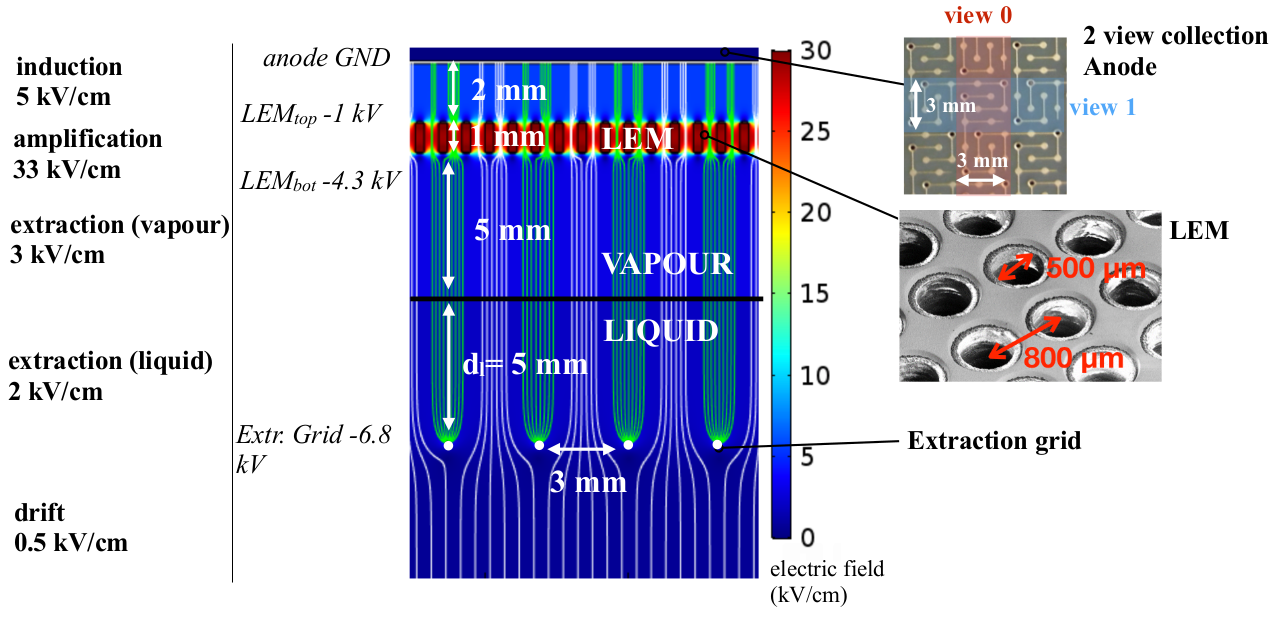
\includegraphics[width=\textwidth,keepaspectratio]{crp_fields.png}\end{center}
%                \caption[Champs électriques d'un  \gls{crp}.]{Illustration des trois principales zones d'un \gls{crp} de \gls{dlartpc}. Les champs et potentiels électriques indiqués correspondent à l'exploitation réussie d'une \gls{dlartpc} ayant atteint des gains effectifs de l'ordre de 20 \cite{Aimard2018,Cantini2014}.}
%                \label{fig::crp_fields}
%            \end{figure}
%            \begin{figure}[htbp]
%                \begin{subfigure}[b]{\textwidth}
%          \begin{center}\includegraphics[width=\textwidth,keepaspectratio]{crp_\TOO{}.png}\end{center}
%          \caption[\gls{crp} du prototype \TOO{}]{Schéma explosé du \gls{crp} du prototype \TOO{}. Les flèches rouges représentent les câbles de suspensions \cite{Aimard2018}.}
%          \label{fig::crp_\TOO{}}
%                \end{subfigure}
%                \begin{subfigure}[b]{\textwidth}
%          \begin{center}\includegraphics[width=\textwidth,keepaspectratio]{crp_\SSS{}_complete.png}\end{center}
%          \caption[\glspl{crp} du démonstrateur \SSS{}]{Schéma des \glspl{crp} du démonstrateur \SSS{}. L'un d'eux est représenté plus bas pour illustrer le fait qu'il y a 4 \glspl{crp}. Chacun mesure $3\times\SI{3}{\meter\squared}$. Les trais gris verticaux représentent les câbles de suspensions. La grille d'extraction n'est pas représentée sur ce schéma. \cite{CRPdesign}}
%          \label{fig::crp_\SSS{}}
%                \end{subfigure}
%                \caption{Schéma des \glspl{crp} de \protodp{}}
%            \end{figure}
%        
%            Le \gls{crp} a pour rôle:
%            \begin{enumerate}
%                \item L'extraction depuis l'argon liquide vers l'argon gazeux des électrons de dérives
%                \item L'amplification de ces électrons
%                \item La collecte du signal ainsi créé
%            \end{enumerate}
%            Toutes ces étapes sont réalisées grâce à trois champs électriques différents:
%            \begin{enumerate}
%                \item Le champ d'extraction, créé par une différence de potentielle entre la grille d'extraction et le bas du dispositif d'amplification. Sa mission est d'extraire un maximum d'électron du liquide vers le gaz en un temps aussi court que possible.
%                \item Le champ d'amplification, créé par une différence de potentielle à travers le dispositif d'amplification
%                \item Le champ d'induction, créé par un différence de potentiel entre le haut du dispositif d'amplification et les anodes de lecture
%            \end{enumerate}
%            La \autoref{fig::crp_fields} résume les points suivants : la grille d'extraction se situe $\SI{5}{\milli\meter}$ sous le niveau d'argon liquide, le bas du dispositif d'amplification se situe $\SI{5}{\milli\meter}$ au dessus du liquide. La tension appliquée entre les deux de $\SI{2.5}{\kilo\volt}$ correspondant à un champ électrique dans le liquide de $\SI{2}{\kilo\volt\per\centi\meter}$ ($\SI{3}{\kilo\volt\per\centi\meter}$ dans le gaz). Une étude \cite{guschin} a montré qu'à ces tensions, la totalité des électrons peut être extraite du liquide vers le gaz.
            
%            Le dispositif d'amplification est un ensemble de plusieurs \glspl{lem}, décrits en détails en \autoref{sec::LEM}, d'une épaisseur de $\SI{1}{\milli\meter}$ à travers laquelle est appliquée une tension de $\SI{3.5}{\kilo\volt}$, correspondant à un champ électrique d'environ $\SI{35}{\kilo\volt\per\centi\meter}$. De précédentes expériences \cite{Badertscher2011,Cantini2014} ont montré qu'un gain de l'ordre de 20 est atteignable à cette tension.
            
%            Les anodes, décrites en \autoref{sec::anode}, sont situées $\SI{2}{\milli\meter}$ au dessus des \glspl{lem}. Une tension de $\SI{1}{\kilo\volt}$ entre les anodes et le haut des \glspl{lem} créé un champ d'induction de $\SI{5}{\kilo\volt\per\centi\meter}$, qui doit alors correspondre à un probabilité de collection de charge optimale (voir \autoref{sec::efficacites}).
            
%            Les \glspl{lem} et anodes sont fixés sous des supports en fibre de verre G10, eux même fixés sous un squelette en acier inoxydable pour le prototype \TOO{} ou en Invar pour le démonstrateur \SSS{} (voir \autoref{sec::crp_structure}). La grille d'extraction est constituée de fils d'acier inoxydable, chacun tendu à $\SI{1.5}{\newton}$ à température ambiante sur des \glspl{pcb}, eux même fixés sur les bords des supports en G10. Le \gls{crp} est désolidarisé du reste du cryostat, il est donc possible de l'assembler et de le tester à part. Un système de câbles et poulies permet d'ajuster la position du \gls{crp} au dessus du liquide. La \autoref{fig::crp_\TOO{}} et la \autoref{fig::crp_\SSS{}} montrent respectivement le \gls{crp} du prototype \TOO{} et un \gls{crp} du démonstrateur \SSS{}. Le prototype \TOO{} n'a qu'un \gls{crp} recouvrant toute sa surface, mais le démonstrateur \SSS{} a quatre \gls{crp} de $3\times\SI{3}{\meter\squared}$, indépendants entre eux. Due à des retards de production, seuls deux de ces \gls{crp} sont instrumentés. Sur les deux autres, les \glspl{lem} et anodes ont été remplacés par des \glspl{pcb} mis à la masse.
%            
%            Le \gls{crp} est munie de plusieurs capteurs de pression, de température ainsi que de niveau d'argon liquide afin de suivre en direct les conditions à l'intérieur du détecteur et de pouvoir ajuster le niveau du \gls{crp} par rapport au liquide.
        
%    \subsection{Les contraintes techniques et la structure}\label{sec::crp_structure}
%            
%            Le \gls{crp} doit respecter plusieurs contraintes techniques \cite{CRPdesign} pour permettre une lecture efficace et fidèle de la charge:
%            
%            \begin{itemize}
%                \item Il doit être le plus plat possible, afin que l'interface liquide-gaz si situe bien au milieu de la distance grille--\gls{lem} pour tout le \gls{crp}. La tolérance fixée pour le démonstrateur \SSS{} est de \SI{0.5}{\milli\meter}, celle atteinte dans le prototype \TOO{} est de \SI{1}{\milli\meter} \cite{Aimard2018}.
%                \item Il doit supporter des variations de température importante sans se déformer de manière significative : le \gls{crp} est assemblé à température ambiante et descend ensuite à mois de \SI{90}{\kelvin}
%                \item Il doit être possible d'ajuster la position du \gls{crp} par rapport au niveau d'argon liquide à \SI{0.05}{\milli\meter} près.
%                \item Le démonstrateur \SSS{} est constitué de 4 \gls{crp}. La distance entre eux doit être de \SI{10}{\milli\meter} maximum
%                \item Comme le \gls{crp} est assemblé à part du reste du détecteur, il doit être transportable
%                \item Le \gls{crp} du démonstrateur \SSS{} doit être un élément utilisable dans la future expérience \gls{dune}, dont un module de détection sera constitué d'une trentaine de ces \gls{crp}
%            \end{itemize}
%            
%            Afin de satisfaire ces contraintes, la structure principale des \glspl{crp} du démonstrateur \SSS{} est faite en Invar, un alliage de fer et de nickel dont le coefficient de dilatation thermique est particulièrement faible (\SI{1.5e-6}{\per\kelvin} entre \SI{22}{\celsius} et \SI{-186}{\celsius}). La structure du \gls{crp} du prototype \TOO{} est elle faite en acier inoxydable.
%            
%            Les \glspl{lem} et anodes sont montés sur des cadres en G10 (neuf dans le \SSS{} et trois dans le \TOO{}), de la fibre de verre feuilletée solide et électriquement isolante. Des mesures de contraction thermique réalisées en 2015 ont donné pour le G10 utilisé dans \protodp{} des coefficients de l'ordre de \SI{e-5}{\per\kelvin}, proches du ceux des \glspl{las}. Le G10 et les \glspl{las} réagissent donc de la même manière aux différents changements de température. Sur les trois mètres du \gls{crp} du démonstrateur \SSS{}, la contraction maximum mesurée est d'environ \SI{6}{\milli\meter}. L'Invar se contractant beaucoup moins, les cadres en G10 sont fixés sur la structure en Invar avec des éléments permettant au G10 de se contracter librement.
%            
%            Le positionnement vertical et horizontal des \glspl{crp} se fait grâce à un système de suspension. Un \gls{crp} (dans le \SSS{} comme dans le \TOO{}) est suspendu par trois câbles motorisés, passant par des conduites isolantes traversant le couvercle du détecteur pour atteindre le \gls{crp}. Ils permettent une amplitude verticale de \SI{98}{\milli\meter} dans le démonstrateur \SSS{} (\SI{40}{\milli\meter} dans le prototype \TOO{}) avec une précision de \SI{100}{\micro\meter} et une amplitude horizontale de \SI{26}{\milli\meter} dans le démonstrateur \SSS{}. Le \TOO{} n'est pas pourvu d'un système de positionnement horizontal.
%            
%            Les \glspl{las} sont assemblés et fixés sur le cadre en G10 par des entretoises en PEEK (polyétheréthercétone) assurant l'espacement de \SI{2}{\milli\meter} entre les \glspl{lem} et les anodes. Les extrémités de ces entretoises sont filetées, un côté est vissé directement dans le G10.
            
%    \subsection{Électronique : signaux, alimentation}
%            
%            Les signaux sont apportés vers l'extérieur par des conduites similaires à celles des câbles de suspension, remplies d'azote \cite{Acciarri2016a} traversant le couvercle du détecteur. Elles sont faites de manière à ce que l'électronique Frontend soit accessible pour d'éventuelles réparations sans contaminer l'argon. Les cartes Frontend (des circuits CMOS ASIC) sont située en bas des conduites et refroidie à \SI{110}{\kelvin}. L'électronique numérique et le \gls{daq} sont situés en dehors du cryostat.
%            
%            L'alimentation haute tension passe elle aussi par des conduites isolante, et est distribuée aux \gls{lem}, aux anodes et à la grille d'extraction par des câbles coaxiaux courant le long de la structure du \gls{crp}. Dans le prototype \TOO{}, chaque face de chaque \gls{lem} ainsi que chaque anode a sa propre alimentation. Dans le démonstrateur \SSS{}, les faces hautes des \glspl{lem} sont alimentées par groupe de neuf.
%            
%            Les anodes sont reliées entre elles via des nappes et des connecteurs KEL formant des canaux de trois mètres de long dans le \SSS{} et trois ou un mètre dans le \TOO{}.
%            
    \subsection{Les anodes}\label{sec::anode}
        
%            \begin{figure}[htbp]
%                \begin{center}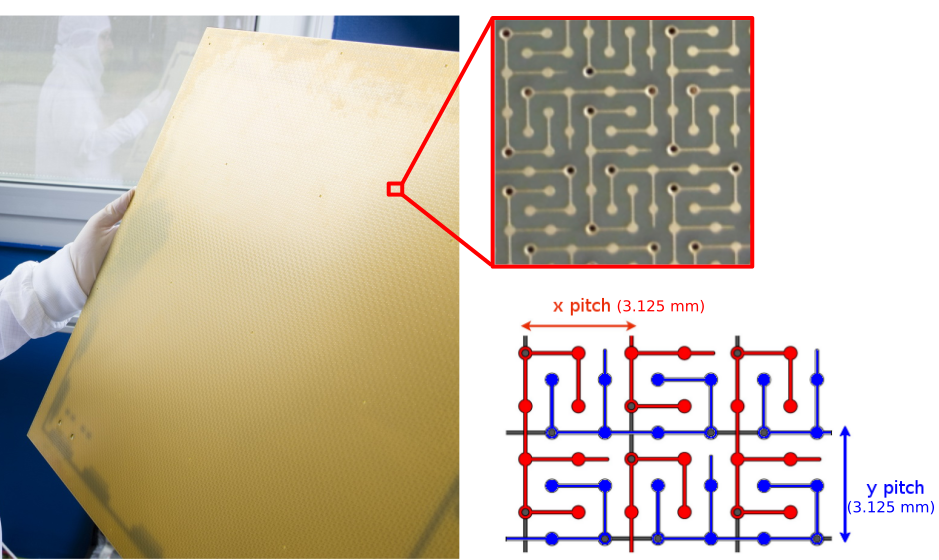
\includegraphics[width=\textwidth,keepaspectratio]{anode.png}\end{center}
%                \caption[Agrandissement d'une anode de lecture.]{Agrandissement d'une anode de lecture. L'orthogonalité des canaux de lecture des vues $x$ et $y$ facilite la reconstruction des événements, la dispositions en plusieurs couches assure une capacitance de $\SI{160}{\pico\farad\per\meter}$ \cite{Cantini2013}.}
%                \label{fig::anode}
%            \end{figure}
%            \begin{figure}[htbp]
%                \begin{center}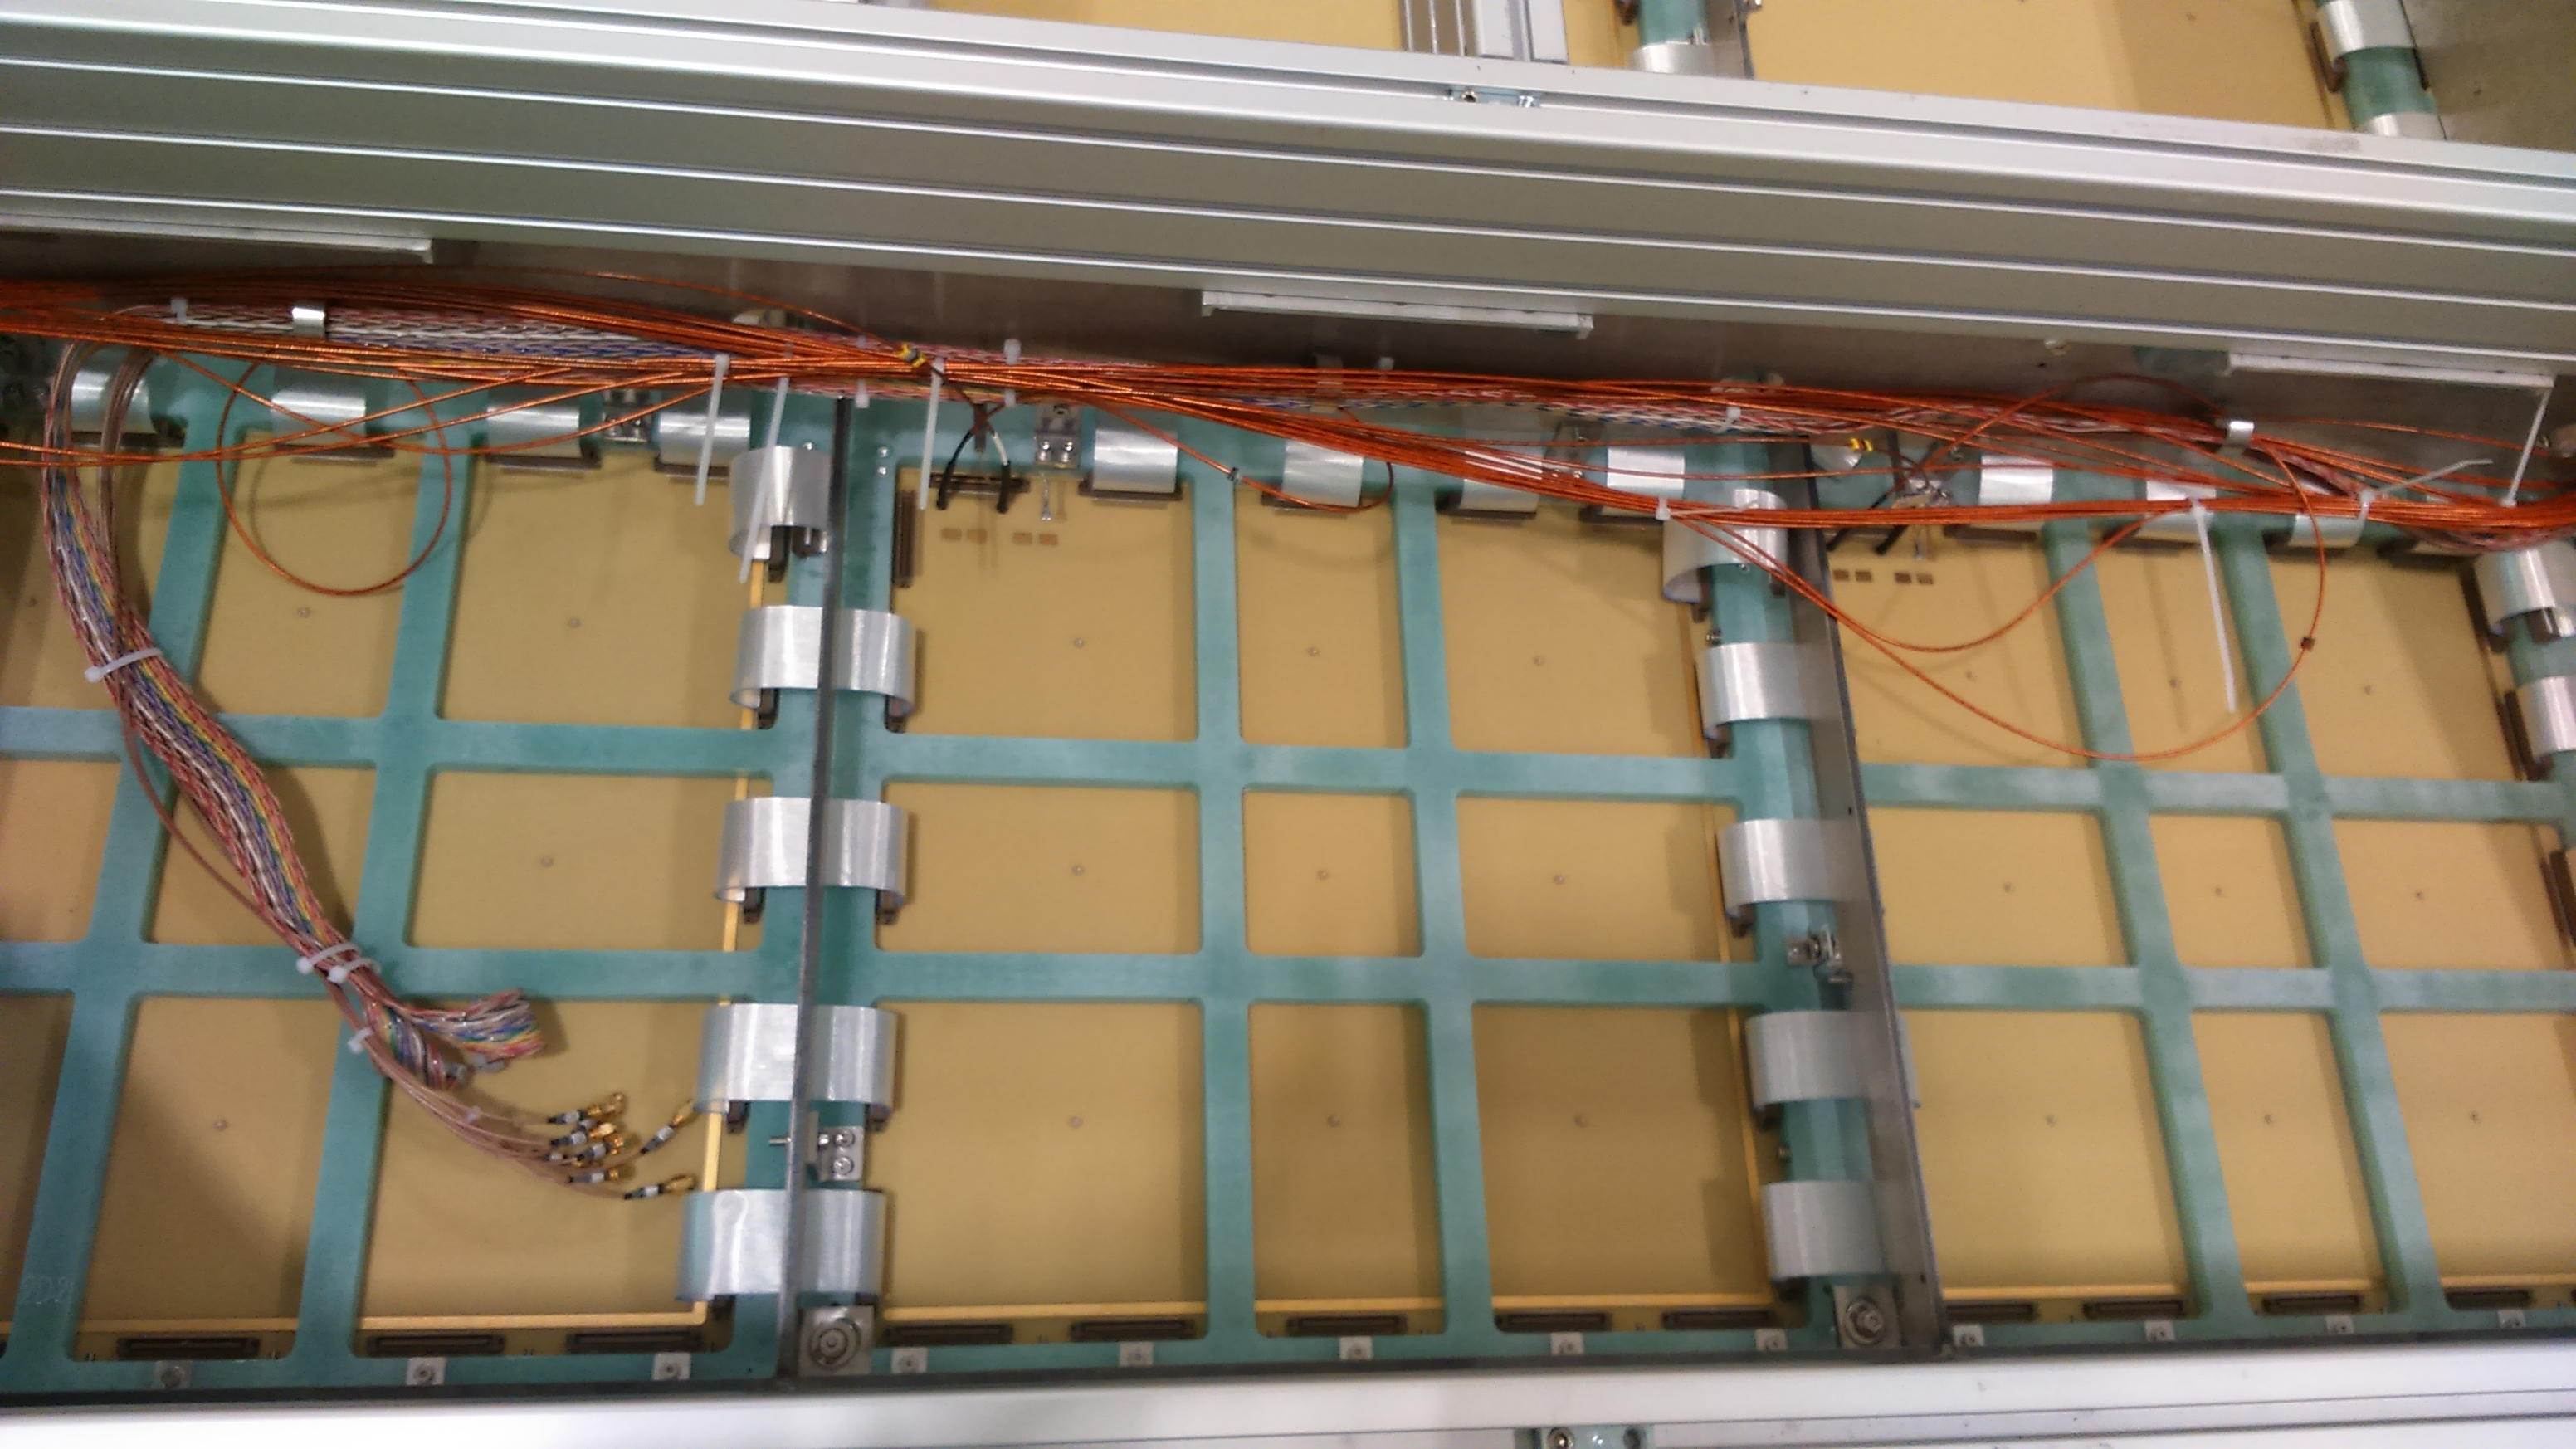
\includegraphics[width=\textwidth,keepaspectratio]{connecteurs2.JPG}\end{center}
%                \caption[Vue du dessus d'un \gls{crp} du démonstrateur \SSS{}.]{Vue du dessus d'un \gls{crp} du démonstrateur \SSS{}. On peut y voir les câbles d'alimentation haute tension des \glspl{lem} le long de la structure en Invar ainsi que les nappes reliant les connecteurs KEL entre les anodes, formant des canaux de \SI{3}{\meter}.}
%                \label{fig::connecteurs}
%            \end{figure}
            
      Le modèle des anodes (voir \autoref{fig::anode}), fabriquées par la compagnie ELTOS\footnote{\url{http://www.eltos.com/en/}} en Italie, est le résultat de tests réalisés au CERN par l'\gls{ethz} dans le prototype de \gls{dlartpc} de \threeL{}\cite{Cantini2013} en vue de réduire au maximum la capacitance, et donc le bruit, tout en ayant un partage égale de charge entre deux vues perpendiculaires, facilitant la reconstruction des événements et leur analyse.
            
      Chaque anode est un \gls{pcb} de quatre couches, avec une surface de  $50\times\SI{50}{\centi\meter\squared}$ et comporte deux jeux de canaux perpendiculaires, \numprint{160} pour la vue $x$ et \numprint{160} pour la vue $y$. La largeur d'un canal est de $\SI{3.125}{\milli\meter}$ et correspond à deux lignes inter-connectées, de cuivre recouvertes d'or. Les canaux sont ramenés par groupes de 32 vers l'autre surface de l'anode jusqu'à des connecteurs KEL de 68 pins, dont les 36 pins restant sont mis à la masse. Dans le prototype de \TOO{} comme dans le démonstrateur de \SSS{}, ces connecteurs sont reliés entre eux d'une anode à l'autre afin de former des canaux continus de $\SI{1}{\meter}$, $\SI{3}{\meter}$ ou $\SI{6}{\meter}$. La capacitance linéique est alors de $\SI{160}{\pico\farad\per\meter}$, correspondant à un bruit de fond inférieur à \numprint{2000} électrons\cite{Aimard2018} pour les longs canaux de $\SI{3}{\meter}$ du prototype de \TOO{}.
            
      Les anodes ont été inspectées visuellement par le fabricant avant envoi, et la continuité de leurs canaux a été testée par Saclay (plus de détails en \autoref{sec::test_anode}).
        
    \subsection{Les Larges Multiplicateurs d'Électrons (LEM)}\label{sec::LEM}

      \begin{figure}[htbp]
        \begin{subfigure}[t]{0.48\textwidth}
          \centering
          \captionsetup{width=.95\linewidth}
          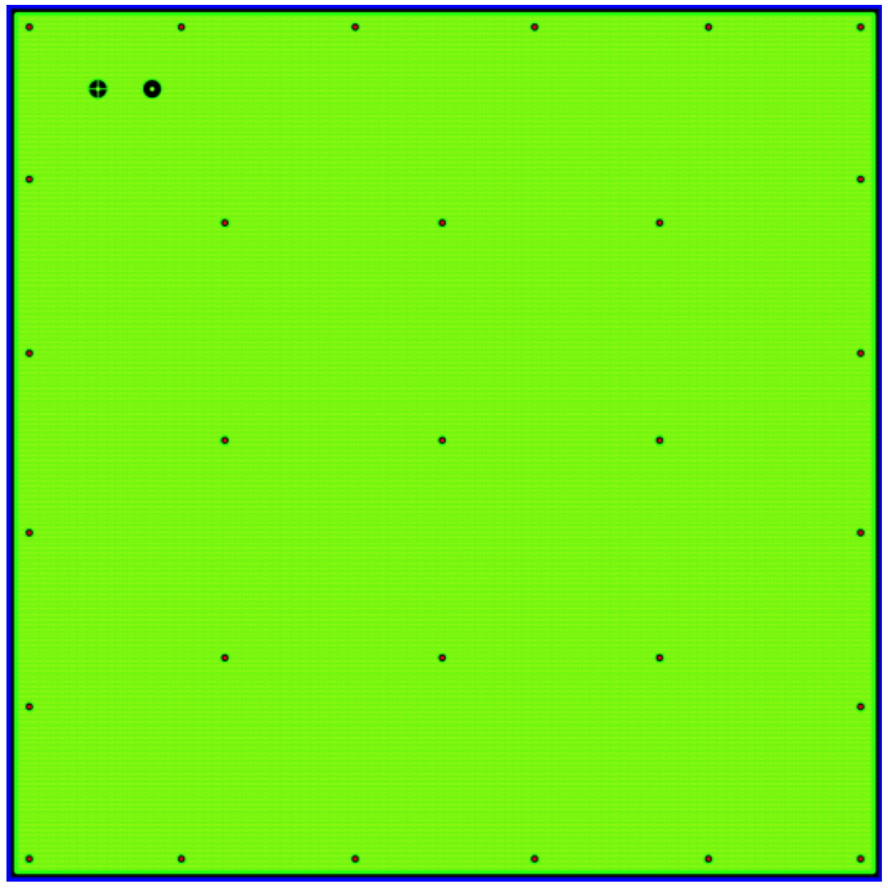
\includegraphics[width=0.8\textwidth,keepaspectratio]{CFR-34.png}
          \caption{\label{fig::cfr34}Modèle de LEM CFR-34 utilisé dans le prototype de \TOO{}. Les zones dépourvues de trous d'amplifications aux bords et autour des trous des vis et des connecteurs haute tension sont plus petites que celles du modèle CFR-35, la surface active totale étant de 96\,\%.}
        \end{subfigure}
        \hfill
        \begin{subfigure}[t]{0.48\textwidth}
          \centering
          \captionsetup{width=.95\linewidth}
          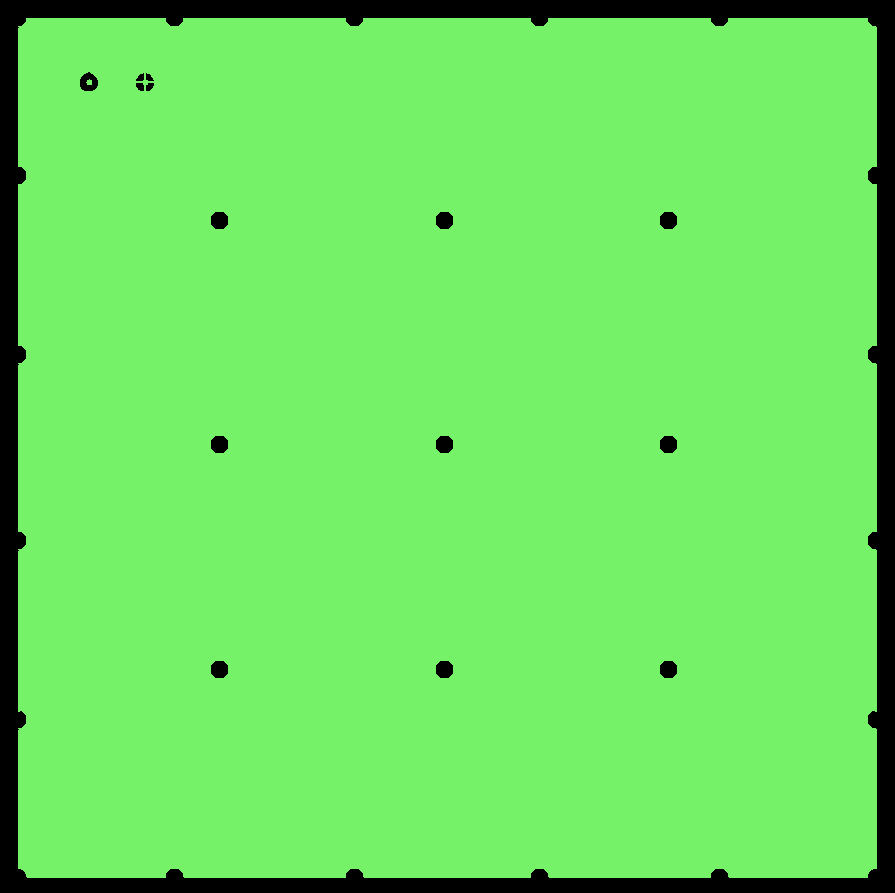
\includegraphics[width=0.8\textwidth,keepaspectratio]{CFR-35.png}
          \caption{\label{fig::cfr35}Modèle de \gls{lem} CFR-35 utilisé dans le démonstrateur de \SSS{}. Les zones dépourvues de trous d'amplifications ont été agrandies par rapport au modèle CFR-34 qui montrait des difficultés à tenir des tensions de l'ordre de \SI{3}{\kilo\volt}, ce qui ne permet pas d'atteindre un gain de 20. Ce nouveau modèle est stable à \SI{3.1}{\kilo\volt}, mais sa surface active totale est réduite à 86\,\%.}
        \end{subfigure}
        \caption[Modèle de LEM CFR-34 et CFR-35]{Fichier Gerber des modèles de \gls{lem} CFR-34 et CFR-35.}
        \label{fig::cfrs}
      \end{figure}

%      Les \glspl{lem} sont l'élément central d'une \gls{dlartpc}. Ce sont eux qui vont permettre l'amplification du signal dans la phase gazeuse. Produits de plusieurs dizaines d'années de recherche et développement, ils ont prouvé être mieux adaptés aux amplifications dans les gaz nobles que les techniques utilisant des chambres à fils, des GEM ou des micro-mégas (\cite{Buzulutskov2000,Breskin2008}). Ce sont des \glspl{pcb} constitués d'une plaque de résine époxy PANASONIC R-1566W (\gls{fr4}) recouverte de chaque côté par une fine couche de cuivre. Des trous sont percés à travers cette plaque, au travers desquelles les électrons primaires, issues de l'interaction d'une particule avec l'argon liquide plus bas, sont accélérés par une forte différence de potentielle appliquée entre les deux couches de cuivre, créant un champ électrique de l'ordre de $\SI{30}{\kilo\volt\per\centi\meter}$. Ceci permet alors de déclencher une avalanche de Townsend (voir \autoref{sec::townsend_avalanche}) et donc d'amplifier le signal.
            
%            Un effet à prendre en compte dans les détecteurs utilisant des amplificateurs comme les \glspl{lem} est le chargement de ces derniers. En effet, les lignes de champs à travers les \glspl{lem} sont tels que des électrons vont pouvoir terminer leur course sur le \gls{fr4} au lieu de traverser le dispositif. Une accumulation de ces électrons diminuera alors le champ d'amplification, entraînant une baisse de gain. Ce phénomène, étudié dans cet article \cite{Cantini2014}, peut être décrit par une décroissance exponentielle du gain à laquelle est associée un temps caractéristique (que l'on appellera temps de charge) qu'il convient de mesurer. Comme une exploitation des résultats n'a vraiment de sens qu'à gain constant, il est préférable de diminuer ce temps de charge afin d'atteindre au plus vite un régime permanent.
            
%            Un autre problème potentielle est que des tensions trop importantes peuvent entraîner des décharges soudaines, entre la grille de un ou plusieurs \gls{lem}, au travers d'un ou plusieurs \gls{lem} ou entre un ou plusieurs \gls{lem} et les anodes. Ces décharges ont, par exemple, grandement limité la prise de données avec le prototype \TOO{} qui n'a pas réussi à atteindre les tensions souhaitées en \autoref{sec::crp_intro}.
            
%      Les \glspl{lem} de \protodp{} ont une surface de $50\times\SI{50}{\centi\meter\squared}$ permettant de couvrir les $\SI{36}{\meter\squared}$ du démonstrateur \SSS{} avec 144 \glspl{lem}, et une épaisseur de $\SI{1}{\milli\meter}$. Ils sont percés de \numprint{400000} trous de $\SI{500}{\micro\meter}$ de diamètre, répartis selon un motif hexagonale sur la surface du \gls{lem} (voir \autoref{fig::lem}). Chaque trou est entouré d'un anneau dépourvu de cuivre d'une épaisseur de $\SI{40}{\micro\meter}$ appelé rim, servant à assurer la stabilité en tension du \gls{lem}\cite{Breskin2008}. L'épaisseur de cuivre est de $\SI{60}{\micro\meter}$. Les \glspl{lem} sont percés de \numprint{29} trous de fixation au travers desquelles passent les entretoise et deux trous pour passer les connecteurs haute tension. Les spécifications précises sont décrites dans le \autoref{tab::lem_commun}.
            
      Les \glspl{lem} utilisés dans le prototype de \TOO{} ont un bord dépourvu de cuivre de $\SI{2}{\milli\meter}$, suivi d'un bord de $\SI{2}{\milli\meter}$ de cuivre dépourvu de trous d'amplification. Des zones similaires sont présentes également autour des trous de fixation et des connecteurs haute tension. Les effets de ces zones sur la collection de charge et la résolution en énergie est présentée en \autoref{sec::dead_zones}. Des tests de tenue en haute tension effectués à Saclay (voir \autoref{sec::test_HT}) sur les \glspl{lem} destinés au démonstrateur de \SSS{} ont permis de montrer que ce modèle (appelé CFR-34) ne permettait pas d'atteindre la tension de \SI{3.1}{\kilo\volt} qui correspond à un gain effectif attendu de 20 (\autoref{fig::3L_gain}). Un nouveau modèle (appelé CFR-35) a alors été proposé, avec des bords plus larges. Ces derniers sont constitués d'une zone de $\SI{1}{cm}$ dépourvue de cuivre suivi d'une zone de $\SI{5}{mm}$ de cuivre sans trous d'amplification  (voir \autoref{fig::cfrs}). C'est ce modèle qui a été choisi pour le démonstrateur \SSS{}. Les spécifications précises des deux modèles sont décrites dans le \autoref{tab::lem_diff}.
            
      \begin{table}
        \centering
        \begin{tabular}{|l|c|c|}
          \hline
           & valeur & tolérance \\
          \hline
          Épaisseur d'époxy & \SI{1}{\milli\meter} & \\
          Épaisseur de cuivre & \SI{60}{\micro\meter} & \\
          Couche de finition & \SI{5}{\micro\meter} Ni$+\SI{0.1}{\micro\meter}$ Au & \\
          Épaisseur totale & \SI{1.065}{\milli\meter} &  $-60/+\SI{20}{\micro\meter}$ \\
          \begin{tabular}{@{}l@{}}Uniformité de \\ l'épaisseur\end{tabular} & $\pm \SI{40}{\micro\meter}$ & \\
          Largeur du RIM & \SI{40}{\micro\meter} & $\pm\SI{4}{\micro\meter}$ \\
          Surface totale &  $499.5\times\SI{499.5}{\milli\meter\squared}$ & $+0/-\SI{0.2}{\milli\meter}$ \\
          Nombre de trous & $\sim400000$ & \\
          Diamètre des trous & $\SI{0.5}{\milli\meter}$ & $-0/+\SI{10}{\micro\meter}$ \\
          \begin{tabular}{@{}l@{}}Distance centre à \\ centre entre \\ deux trous\end{tabular}  & $\SI{0.8}{\milli\meter}$ & \\
          \hline
        \end{tabular}
        \caption[Caractéristiques des LEMs communes aux deux modèles utilisés dans WA105]{\label{tab::lem_commun}Caractéristiques des \glspl{lem} communes aux deux modèles utilisés dans \gls{wa105}.}
      \end{table}
            
      \begin{table}
        \centering
        \begin{tabular}{|l|c|c|}
          \hline
           & CFR-34 & CFR-35\\
          \hline
          Bord -- zone sans cuivre & \SI{2}{\milli\meter} & \SI{10}{\milli\meter}\\
          Bord -- zone avec cuivre sans trous & \SI{2}{\milli\meter} & \SI{5}{\milli\meter}\\
          Trous de vis -- diamètre sans cuivre & \SI{4.2}{\milli\meter} & \SI{10}{\milli\meter} \\
          Trous de vis -- anneau sans trous &  \SI{1.1}{\milli\meter} & \SI{5}{\milli\meter} \\
          Trous de connecteur -- diamètre sans cuivre & \SI{10}{\milli\meter} & \SI{10}{\milli\meter} \\
          Trous de connecteur -- anneau sans trous & \SI{1}{\milli\meter} & \SI{5}{\milli\meter} \\
          \hline
        \end{tabular}
        \caption[Caractéristiques spécifiques aux modèles de LEM utilisés dans \protodp{}]{\label{tab::lem_diff}Caractéristiques spécifiques aux modèles de \gls{lem} utilisés dans \protodp{}.}
      \end{table}

  \section{Préparation, caractérisation et test à l'IRFU et au CERN}
    
    Le \gls{cea} Saclay était en charge de la production et les tests des des \glspl{lem} des deux \glspl{crp} instrumentés démonstrateur de \SSS{}, ainsi que les tests des anodes de ces même \glspl{crp}. Un appel d'offre pour les modèles a été lancé en février 2017 et l'entreprise ELTOS a été retenue. Il a été demandé à l'entreprise d'effectuer plusieurs mesures sur les \glspl{lem} produits : l'épaisseur de la plaque d'époxy et des couches de cuivre, l'épaisseur des RIMs, la taille des trous d'amplification ainsi que les caractéristiques diélectriques. Le \gls{cea} a par la suite effectué des mesures complémentaires de l'épaisseur totale, ce paramètre ayant un impact particulièrement important sur le gain (voir \autoref{sec::townsend}). Des tests de tenus en haute tension ainsi que des mesures de gain avec une source radioactive dans de l'argon gazeux à densité équivalente à celle de la phase gazeuse d'une \gls{dlartpc} ont été réalisés dans une enceinte haute pression construite dans ce but. Enfin, des tests de continuité des canaux de lecture des anodes ont également été réalisés.
        
    \subsection{Production et préparation des LEM}
        
      La réalisation d'un \gls{lem} par ELTOS commence par un perçage des plaques d'époxy préalablement couvertes de cuivre, avec changement fréquent des forets. S'en suit un nettoyage des résidus d'époxy et de métal dans les trous, puis un polissage pour arrondir les bords des trous. Les RIMs sont obtenus par micro-etching. Un traitement de surface nickel/or est appliqué. Le \gls{lem} est détouré à ses dimensions finales  et les zones mortes sur les bords sont réalisées par gravure chimique. Enfin, le \gls{lem} est nettoyé, rincé et étuvé.
          
      Sont ensuite effectuées les mesures décrites en \autoref{sec::thickness_comparison_eltos} pour s'assurer de la conformité au cahier des charges.
      
      Entre juillet 2017 et septembre 2018, le \gls{cea} a reçu et testé les 72 \glspl{lem} du démonstrateur \SSS{}. Une fois les \glspl{lem} arrivés à l'\gls{irfu}, ils sont inspectés visuellement et les imperfections sont relevées. Ils sont ensuite envoyés à la métrologie afin que leurs épaisseurs soient mesurées (voir \autoref{sec::epaisseur}).
      
      L'étape suivante est alors la soudure de connecteurs haute tension et le collage des entretoises en MACOR, qui permettront d'assurer une distance entre le \gls{lem} et l'anode de \SI{2}{\milli\meter}.
      
      \SI{24}{\hour} après le collage, les \glspl{lem} sont nettoyés pendant \numprint{3} minutes dans un bain à ultrasons d'eau désionisée et de lessive, à \SI{65}{\celsius} puis rincés d'abord à l'eau claire puis au Karcher avec de l'eau désionisée. Ils sont ensuite séchés une première fois avec un jet l'azote avant d'être séchés une seconde fois au four à \SI{80}{\celsius} pendant \numprint{3} heures. Ils sont ensuite polymérisés au four à \SI{160}{\celsius} pendant \numprint{3} heures.

      Ils sont ensuite placés dans une enceinte haute pression. Cette enceinte est dans un premier temps remplie d'air sec, ou une tension de \SI{4500}{\volt} est appliquée à travers le \gls{lem} afin de détruire les micro-poussières restantes. L'air sec est ensuite remplacé par de l'argon gazeux à \SI{3.3}{\bar}, recréant ainsi la densité de la phase gazeuse d'une \gls{dlartpc}. Sont alors effectués des tests de tenus en tension et des mesures de gain (voir \autoref{sec::test_HT}).
        
    \subsection{Les mesures d’épaisseur des LEM}\label{sec::epaisseur}
        
      \subsubsection{Motivation : impact sur le gain}
            
        \begin{figure}[htbp]
          \centering
          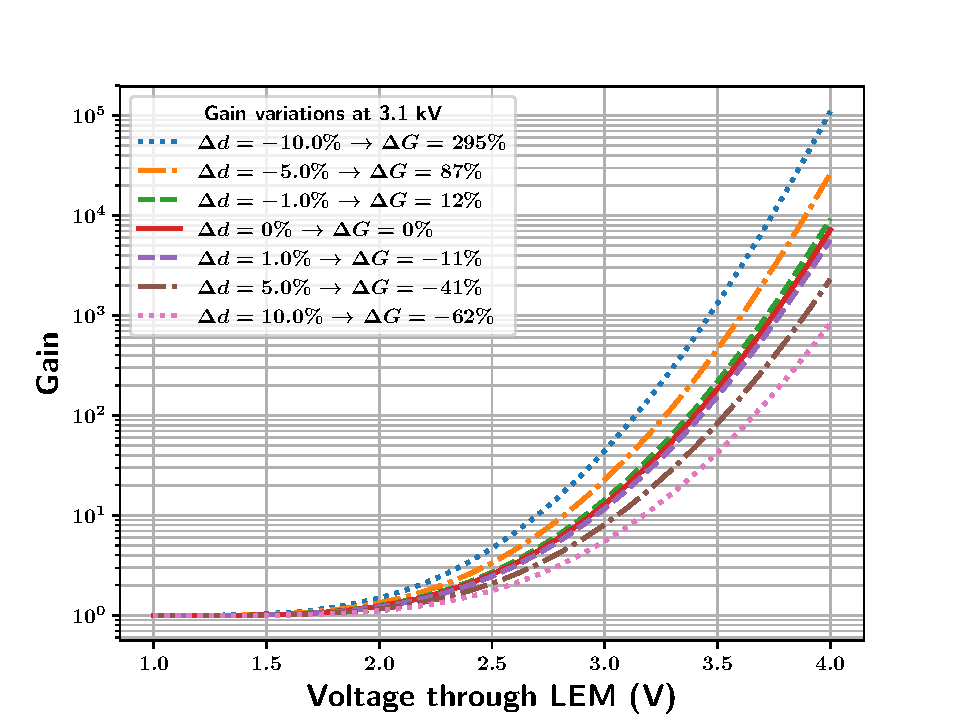
\includegraphics[width=0.8\textwidth,keepaspectratio]{influence_dx_gain.pdf}
          \caption[Influence de l'épaisseur d'un LEM sur le gain]{Influence attendue de l'épaisseur d'un \gls{lem} sur le gain, d'après le formule \eqref{eq::townsend_avalanche_2} ajustée aux données présentées dans \cite{Cantini2014}. On constate qu'à \SI{3.1}{\kilo\volt}, une variation de l'épaisseur de 1\,\% entraîne une variation du gain de l'ordre de 10\,\%.}
          \label{fig::thickness_influence_on_gain}
        \end{figure}
            
        La formule du gain à travers un dispositif amplificateur est rappelée ici (voir \autoref{sec::townsend} pour plus de détails) :
        \begin{equation}\label{eq::townsend_avalanche_2}
          G = e^{A\rho d e^{-B\rho /E}}
        \end{equation}
        Avec $\rho$ la densité de l'argon gazeux, $E$ le champ d'amplification dans le \gls{lem}, $A$ et $B$ des constantes dépendant du gaz et $d$ la longueur de la zone d'amplification. Cette longueur $d$ correspond dans le cas d'un \gls{lem} à son épaisseur. Ce paramètre apparaît deux fois, dans la première et dans la seconde exponentielle à travers le champ $E = V/d$, ses variations ont donc un impact significatif sur le gain (voir \autoref{fig::thickness_influence_on_gain}). Il est nécessaire de pouvoir quantifier ses variations pour les \glspl{lem} utilisés, nous avons donc mis en place un dispositif permettant de mesurer l'épaisseur des \glspl{lem} produits pour les deux \gls{crp} du \SSS{}. Les résultats ainsi obtenus sont comparés aux mesures obtenues par le fabricant, ELTOS, dans le \autoref{tab::mesures_eltos}.
                
        \subsubsection{Méthode expérimentale}
                %documentation dans hardware/lem_plaques/marbre_472
          La technique d'\acrfull{cci} (voir \autoref{fig::CCI}), est employée pour mesurer l'épaisseur des \glspl{lem}. L'image $S'$ d'une source polychromatique ponctuelle $S$ est créée à la surface de l'objet à mesurer grâce à une lentille convergente. Les rayons réfléchis en $S'$ retraversent la lentille et sont déviés grâce à un miroir vers un trou d'épingle $S''$, placé devant un spectromètre. La distance focale de la lentille dépend de la longueur d'onde, aussi seul un spectre très restreint de la lumière initiale atteindra le trou d'épingle. En faisant correspondre la longueur d'onde détectée à une distance à la lentille, il est ainsi possible de mesurer la distance entre la lentille et l'objet. Le crayon optique servant de source est monté sur un rail grâce à un chariot à coussin d'air, lui permettant de se déplacer sans frottement sur un axe $x$, dont la coordonnée est enregistrée au micron près. Le logiciel de mesure utilisé permet de visualiser en direct les variations de hauteurs au cours de la mesure. La forme des trous micrométriques des \glspl{lem} est visible sur la \autoref{fig::soft_measure_LEM}, issue de ce logiciel. %A noter que due à l'absence de motorisation du chariot sur coussin d'air, ce dernier était poussé à la main, ce qui ne garantissait pas une vitesse constante.
          
          \begin{figure}[htpb]
            \begin{subfigure}{0.48\textwidth}
              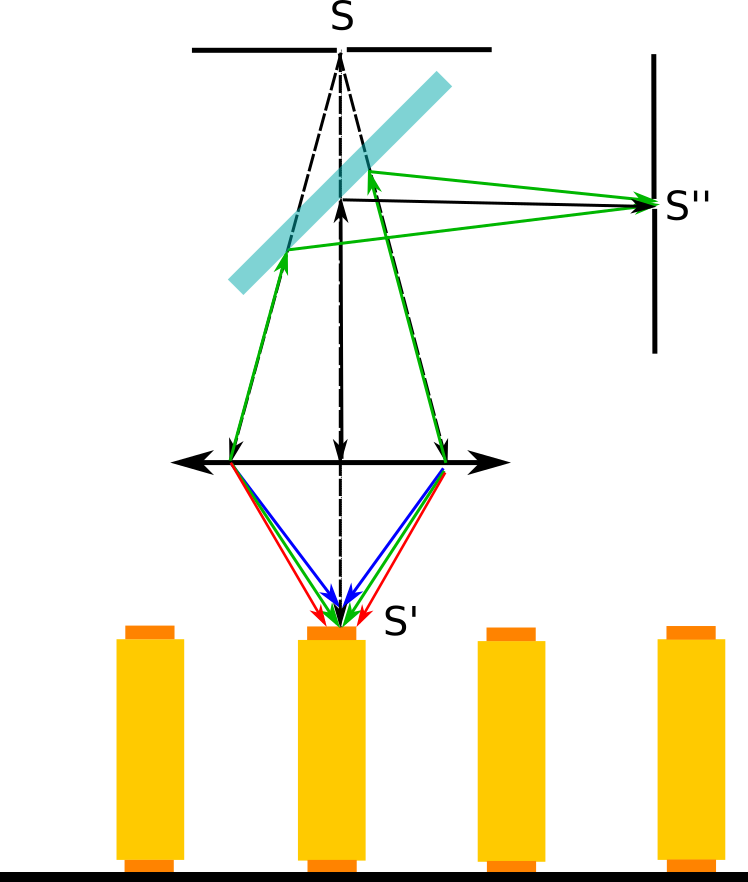
\includegraphics[width=0.8\textwidth,keepaspectratio]{CCI.png}
              \caption{\label{fig::CCI}Schéma de la méthode de mesure \gls{cci} servant à mesurer l'épaisseur des \glspl{lem}. Les blocs oranges et jaunes représentent une vue en coupe, à l'échelle, d'un \gls{lem} posé sur le marbre avec ses trous d'amplification.}
            \end{subfigure}
            \hfill
            \begin{subfigure}{0.48\textwidth}
              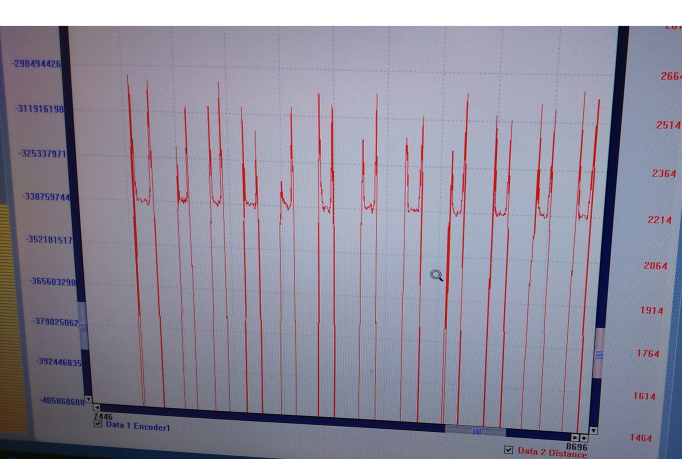
\includegraphics[width=\textwidth,keepaspectratio]{soft_measure_LEM.png}
              \caption{\label{fig::soft_measure_LEM}Représentation brute des données de mesure d'un \gls{lem} avec la technique \gls{cci}. Les grands pics sont coupés à l'analyse.}
            \end{subfigure}
            \caption[Schéma de principe et exemple de mesure de la surface d'un LEM avec la technique CCI]{Schéma de principe et exemple de mesure de la surface d'un \gls{lem} avec la technique \gls{cci}.}
          \end{figure}
          
           Le dispositif mesure la distance entre la surface et le crayon optique. Il faut donc disposer d'une surface plate uniforme sur laquelle poser l'objet à mesurer, qui servira de zéro, et aplatir l'objet. Dans notre cas, le zéro est donné  par un marbre micrométrique. Un exemple de mesure de variations de hauteur de ce marbre est présentée en \autoref{fig::marbre}. On constate que le marbre présente une légère pente, qui peut facilement être prise en compte dans les mesures du \gls{lem}. Le \gls{lem} est aplati par une plaque en acier inox percée de 25 trous à travers lesquels les mesures étaient effectuées, ainsi que des briques de plomb placées le long du chemin de mesure (voir \autoref{fig::plate_and_bricks}). Malgré cela, le trou de mesure situé le plus au centre du \gls{lem} présentait encore des variations de $10$ à $\SI{15}{\micro\meter}$ quand une pression supplémentaire était appliquée sur la plaque d'acier. Il a donc était décidé d'ignorer ce trou de mesure.

          \begin{figure}[htpb]
            \begin{subfigure}[t]{0.5\textwidth}
              \centering
              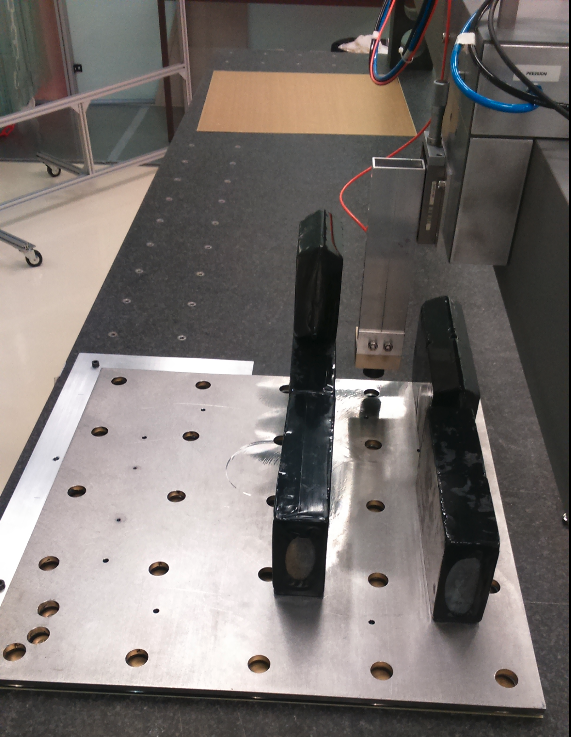
\includegraphics[width=\textwidth,keepaspectratio]{plate_and_bricks.png}
              \caption{\label{fig::plate_and_bricks}Système servant à aplanir le \gls{lem} sur le marbre. Le \gls{lem} est sous une plaque d'acier sur laquelle sont posées des briques de plomb le l'axe de mesure.}
            \end{subfigure}
            \hfill
            \begin{subfigure}[t]{0.395\textwidth}
              \centering
              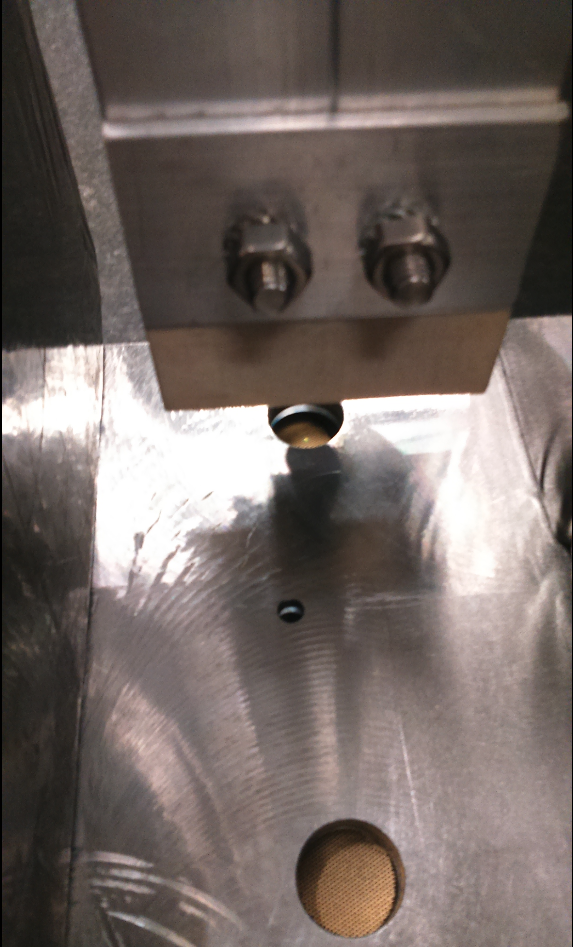
\includegraphics[width=\textwidth,keepaspectratio]{LEM_through_plate.png}
              \caption{\label{fig::LEM_through_plate}Vue du \gls{lem} mesuré à travers un trou de la plaque en acier. Le point vert correspond à la lumière du crayon optique.}
            \end{subfigure}
            \caption[Photographies du dispositif expérimental utilisé pour les mesures d'épaisseur des LEM]{\label{fig::dispositif_experimental}Photographies du dispositif expérimental utilisé pour les mesures d'épaisseur des \glspl{lem}.}
          \end{figure}

          \begin{figure}[htpb]
            \centering
            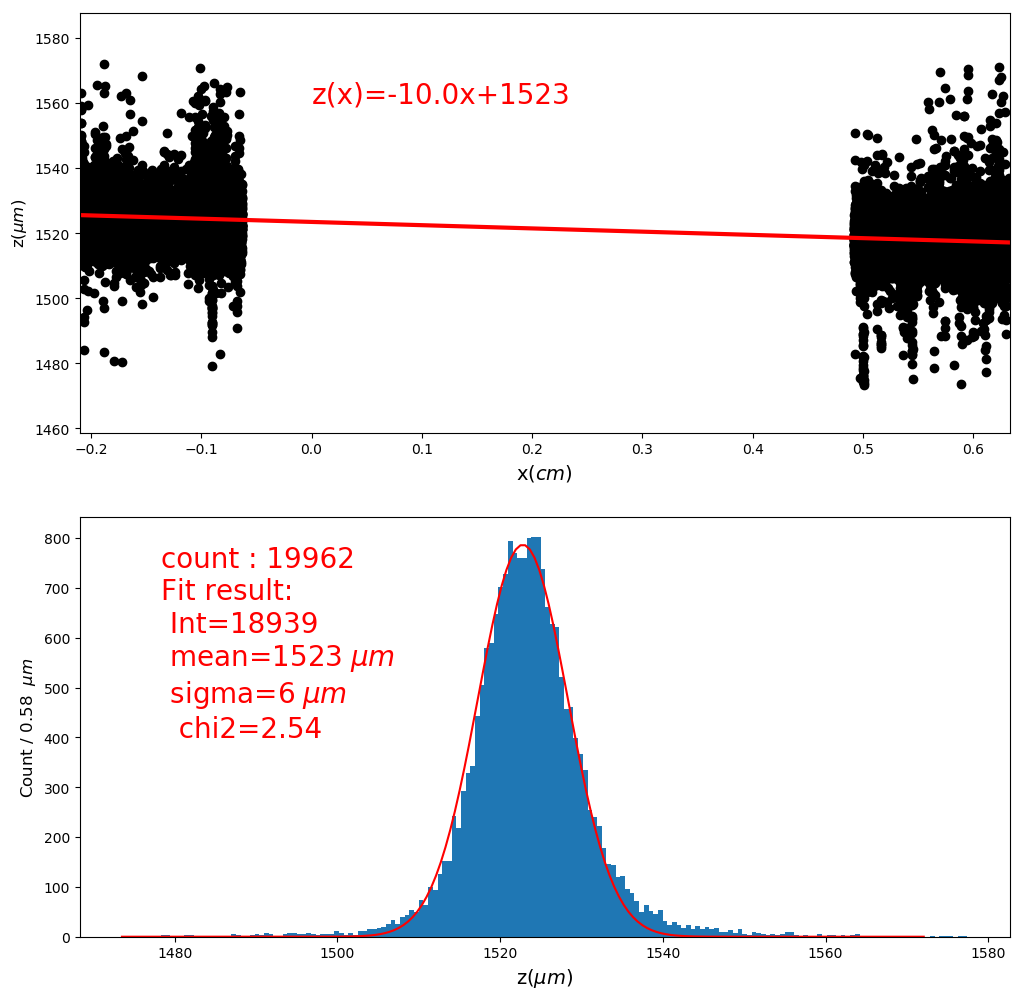
\includegraphics[width=0.8\textwidth,keepaspectratio]{marble.png}
            \caption[Calibration du système de mesure CCI]{\label{fig::marbre}Calibration de la planéité du marbre. Le graphe du haut montre la pente du marbre le long de l'axe de mesure $x$, le graphe du bas montre la dispersion de l'épaisseur du marbre après correction de la pente autour de $x=0$.}
%            \begin{minipage}{0.56\textwidth}
%              \begin{subfigure}[t]{\textwidth}
%                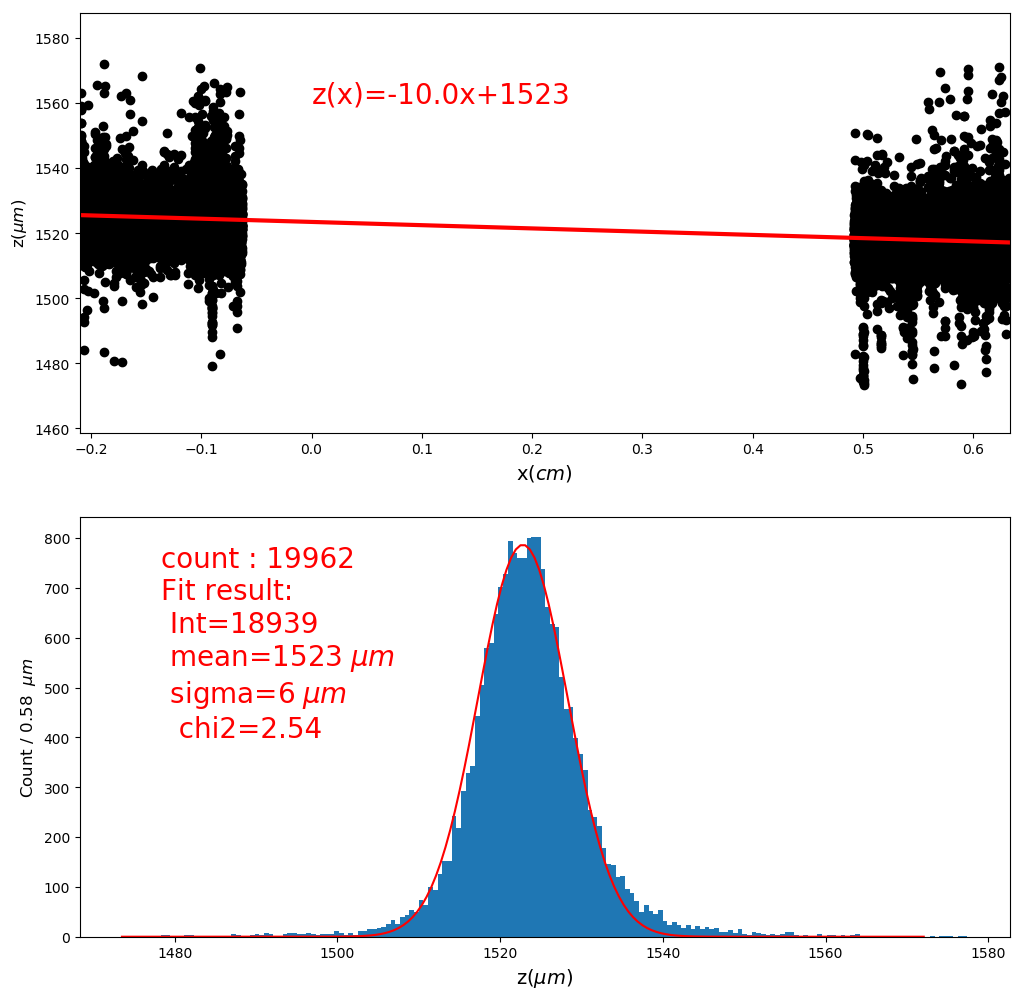
\includegraphics[width=\textwidth,keepaspectratio]{marble.png}
%                \caption{\label{fig::marbre}Calibration du marbre. Le graph du haut montre la pente du marbre le long de l'axe de mesure $x$, le graph du bas montre la dispersion de l'épaisseur du marbre après correction de la pente autour de $x=0$. \textcolor{red}{Je referai ces plots en plus lisible}}
%              \end{subfigure}
%            \end{minipage}
%            \hfill
%            \begin{minipage}{0.38\textwidth}
%              \begin{subfigure}[t]{\textwidth}
%                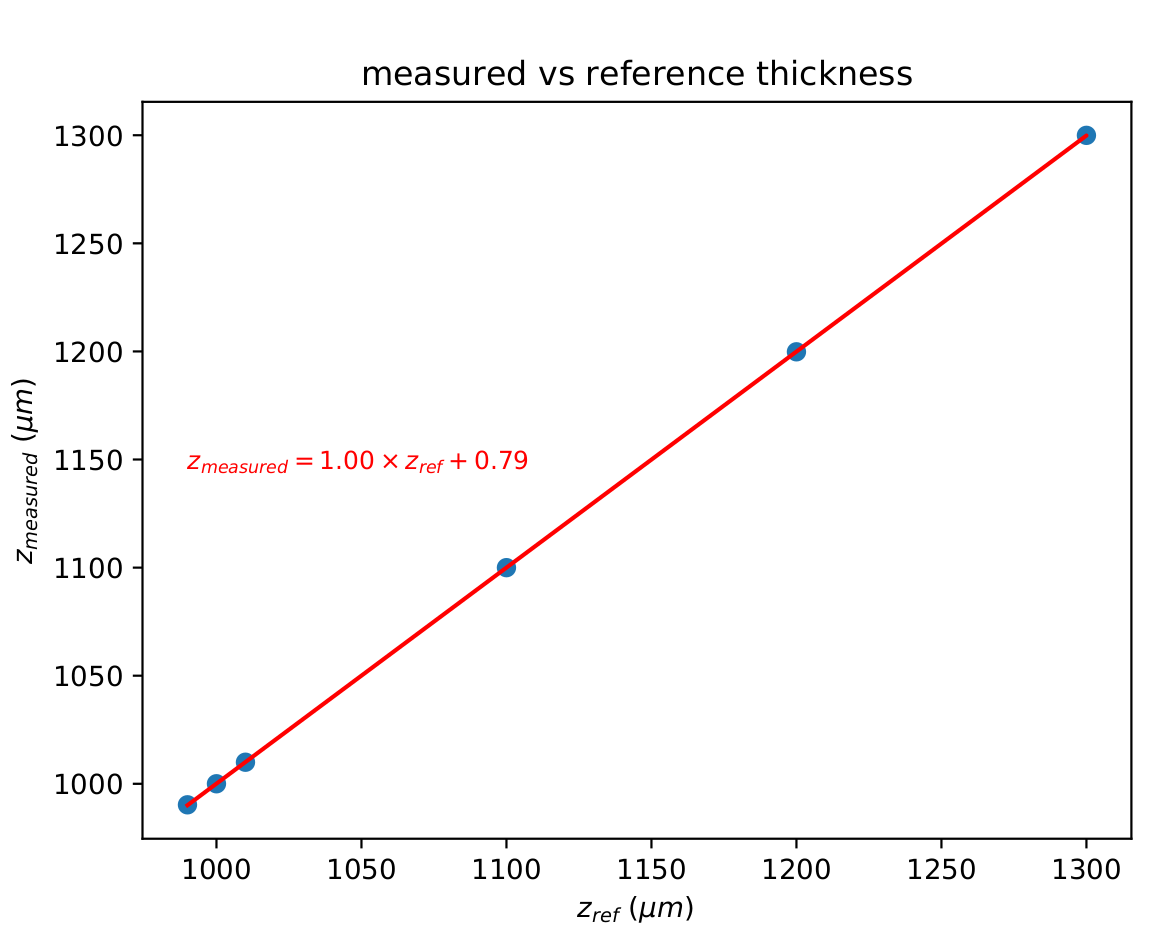
\includegraphics[width=\textwidth,keepaspectratio]{optic_response.png}
%                \caption{\label{fig::optic_response}Calibration de la réponse du crayon optique avec six cales de différentes épaisseurs.}
%              \end{subfigure}
%              \begin{subfigure}[t]{\textwidth}
%                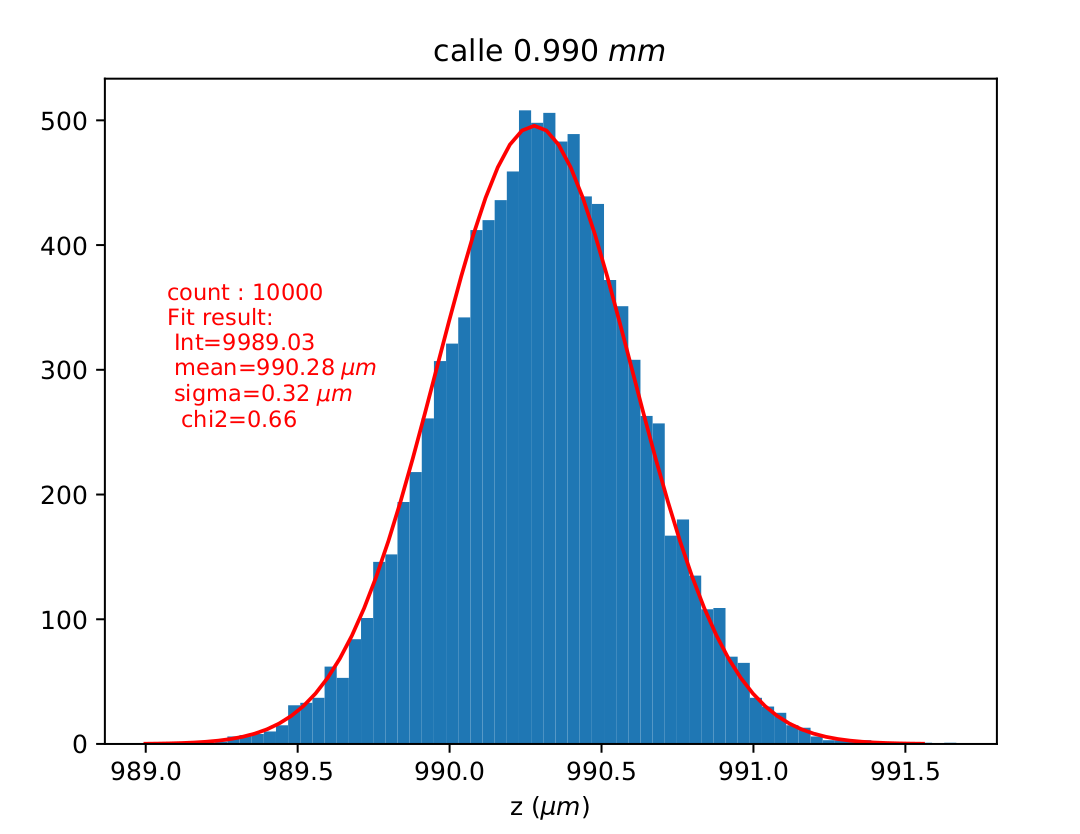
\includegraphics[width=\textwidth,keepaspectratio]{calle.png}
%                \caption{\label{fig::calle}Dispersion de l'épaisseur mesurée d'une cale de \SI{0.99}{\milli\meter}.}
%              \end{subfigure}
%            \end{minipage}
%            \caption[Calibration du système de mesure \gls{cci}.]{\label{fig::calibration}Calibration du système de mesure \gls{cci}.}
          \end{figure}
          Le mouvement selon l'axe $y$ ne peut se faire qu'en déplaçant manuellement la poutre, aussi les mesures ont été prises ligne par ligne. Les mesures sont corrigées pour l'inclinaison du marbre, mesurée à chaque ligne. Celui-ci présentait une pente autour de $\SI{10}{\micro\meter\per\meter}$ (\autoref{fig::marbre}). La moyenne de la distribution des hauteurs du marbre corrigée pour la pente servait de zéro pour les mesures des épaisseurs du \gls{lem} lui même. La réponse du dispositif optique à la hauteur à mesurer a également été calibrée avec des cales d'épaisseur allant de $\SI{900}{\micro\meter}$ à $\SI{1300}{\micro\meter}$.
% en ajustant une droite d'équation $z_{mesure} = \alpha \cdot z_{cale} + \beta$ à la hauteur $z_{mesure}$ mesurée contre la hauteur $z_{cale}$ indiquée sur la cale. Le coefficient $\alpha$ est de $1.00$ et le coefficient $\beta$ de $\SI{0.72}{\micro\meter}$.
          
      \subsubsection{Résultats}\label{sec::thickness_result}
         
        \begin{figure}[htpb]
          \centering
          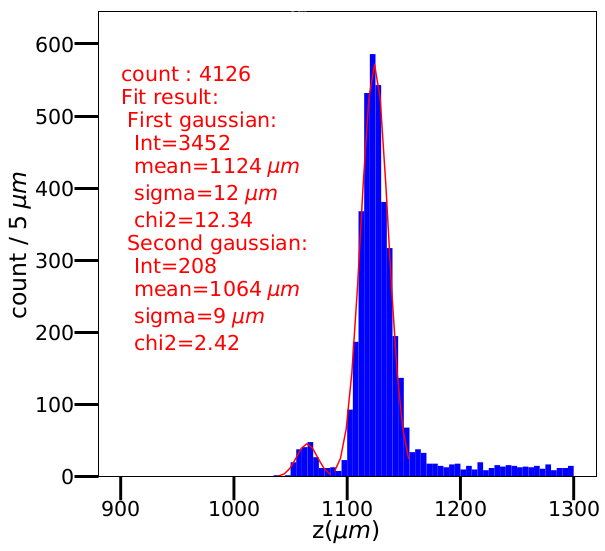
\includegraphics[width=0.5\textwidth,keepaspectratio]{distri_1_trou_lem.png}
          \caption[Exemple de mesure de l'épaisseur d'un LEM]{\label{fig::distri_1_trou_lem}Exemple de mesure de l'épaisseur d'un \gls{lem} à travers un trou de la plaque en acier. Le petit pic de gauche correspond à la lumière réfléchie par le \gls{fr4} du RIM, le pic de droite correspond à la lumière réfléchie par le cuivre.}
        \end{figure}
        \begin{figure}[htpb]
          \centering
          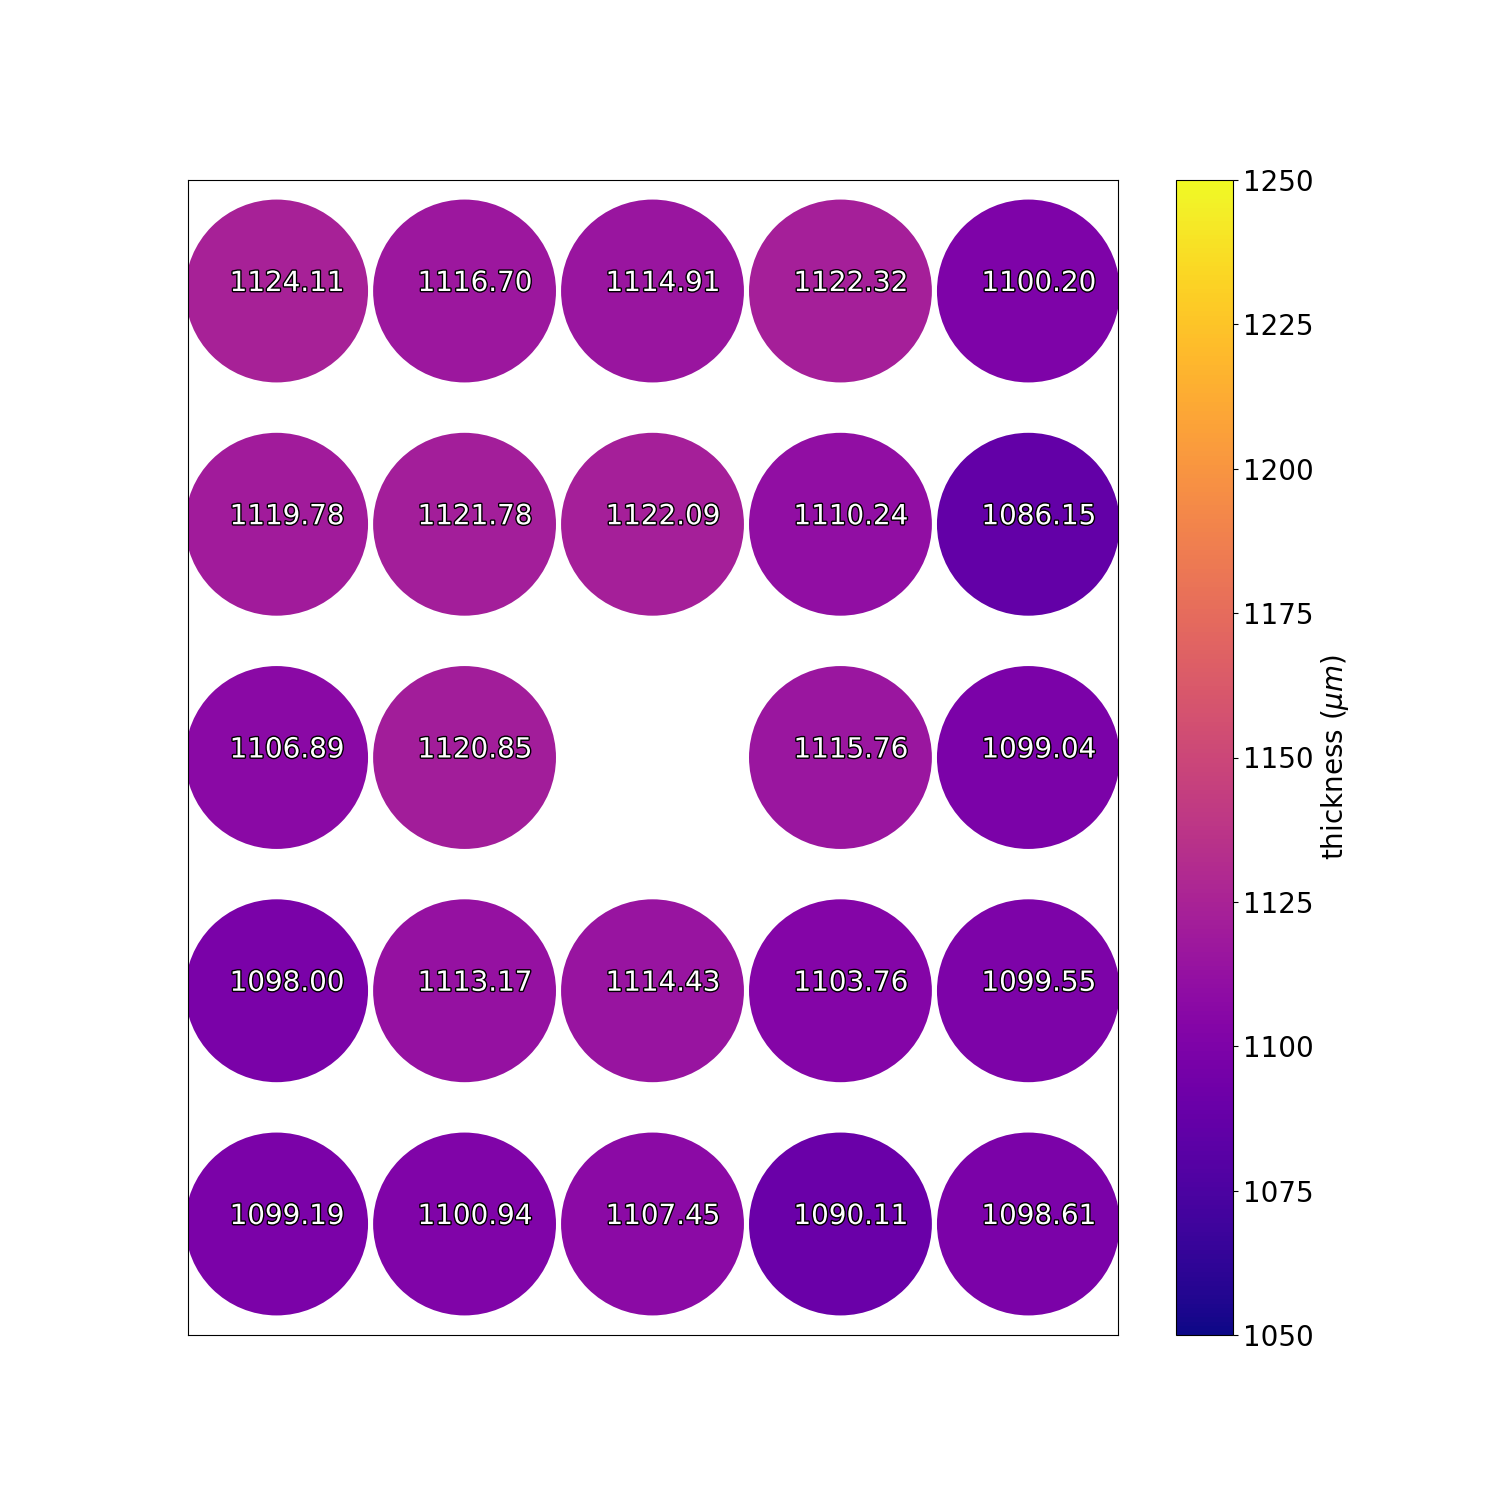
\includegraphics[width=0.5\textwidth,keepaspectratio]{2D_LEM_thickness_distri.png}
          \caption[Uniformité de l'épaisseur d'un LEM]{\label{fig::distri_24_trou_lem_2D}Uniformité de l'épaisseur d'un \gls{lem} mesurée à travers les 24 trous de la plaque d'acier.}
        \end{figure}
          
        \begin{figure}[htpb]
%          \hfill
%          \begin{subfigure}[t]{0.48\textwidth}
%            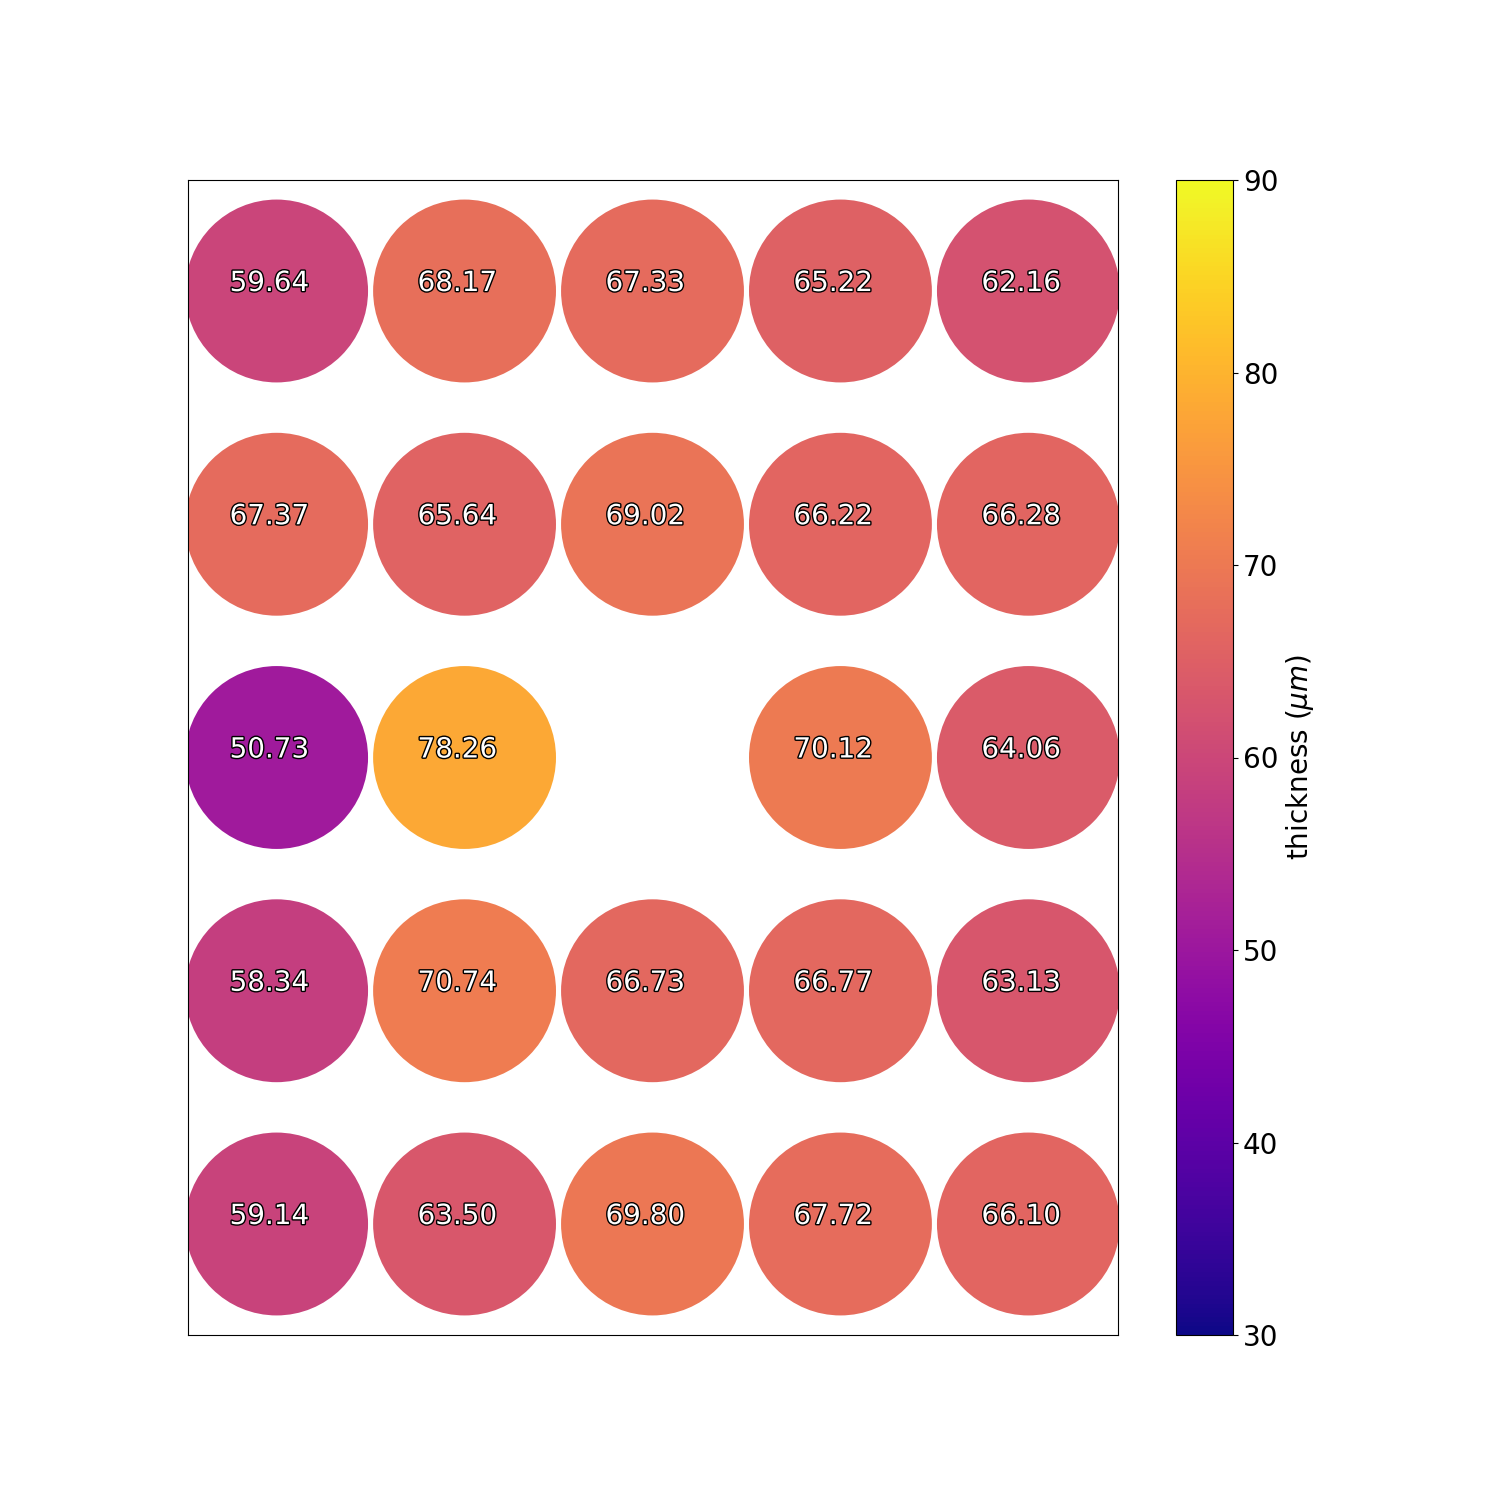
\includegraphics[width=\textwidth,keepaspectratio]{2D_copper_thickness_distri.png}
%            \caption{\label{fig::distri_24_trou_cuivre_2D}Visualisation de la variation d'épaisseur de cuivre d'un \gls{lem} mesurée à travers les 24 trous de la plaque d'acier.}
%          \end{subfigure}\\
          \begin{subfigure}[b]{0.48\textwidth}
            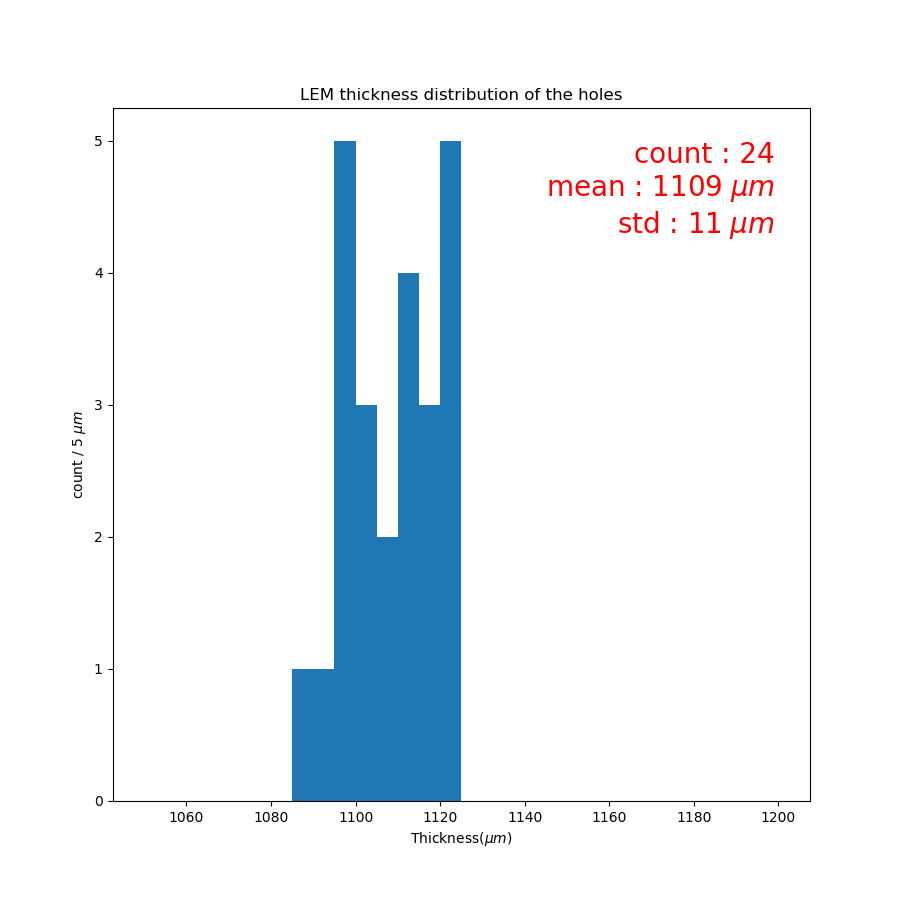
\includegraphics[width=\textwidth,keepaspectratio]{LEM.png}
            \caption{\label{fig::distri_24_trou_lem_1D}Distribution de l'épaisseur totale d'un \gls{lem} mesurée à travers les 24 trous de la plaque d'acier.}
          \end{subfigure}
          \hfill
          \begin{subfigure}[b]{0.48\textwidth}
            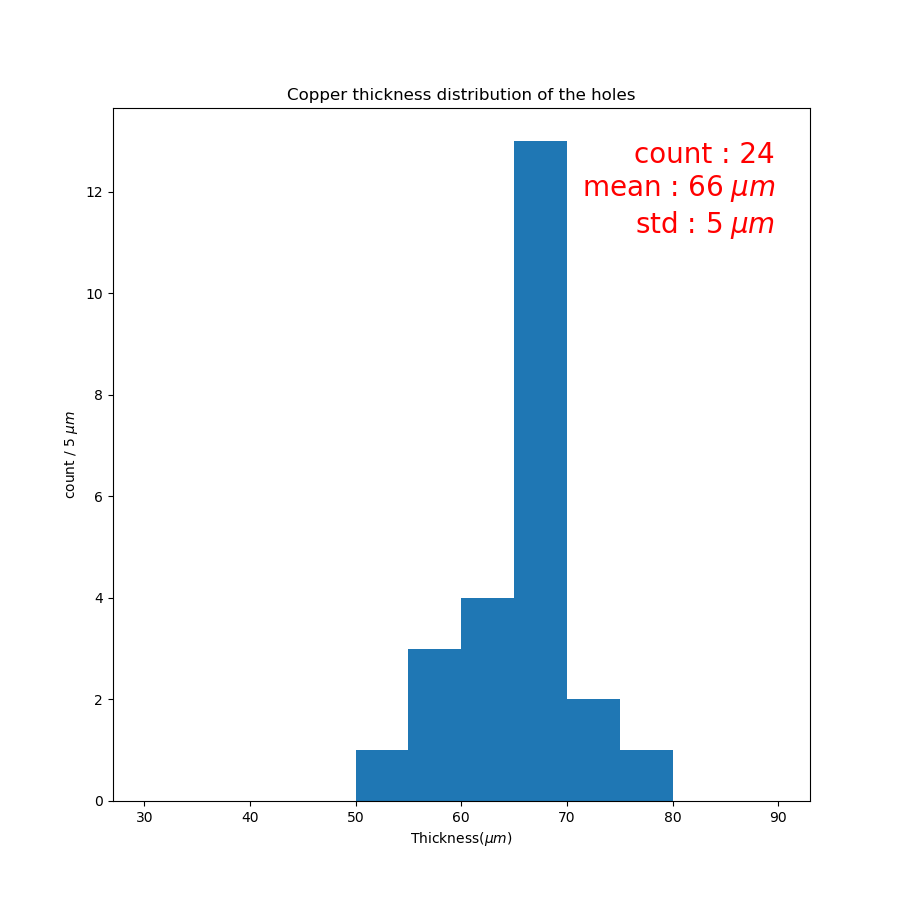
\includegraphics[width=\textwidth,keepaspectratio]{Copper.png}
            \caption{\label{fig::distri_24_trou_cuivre_1D}Distribution de l'épaisseur de cuivre d'un \gls{lem} mesurée à travers les 24 trous de la plaque d'acier.}
          \end{subfigure}
          \caption[Résultats des mesures d'épaisseur pour un LEM]{\label{fig::distri_epaisseur_1_lem}Résultats des mesures d'épaisseur pour un \gls{lem}.}
        \end{figure}
                
        \begin{figure}[htpb]
          \begin{subfigure}[t]{0.48\textwidth}
            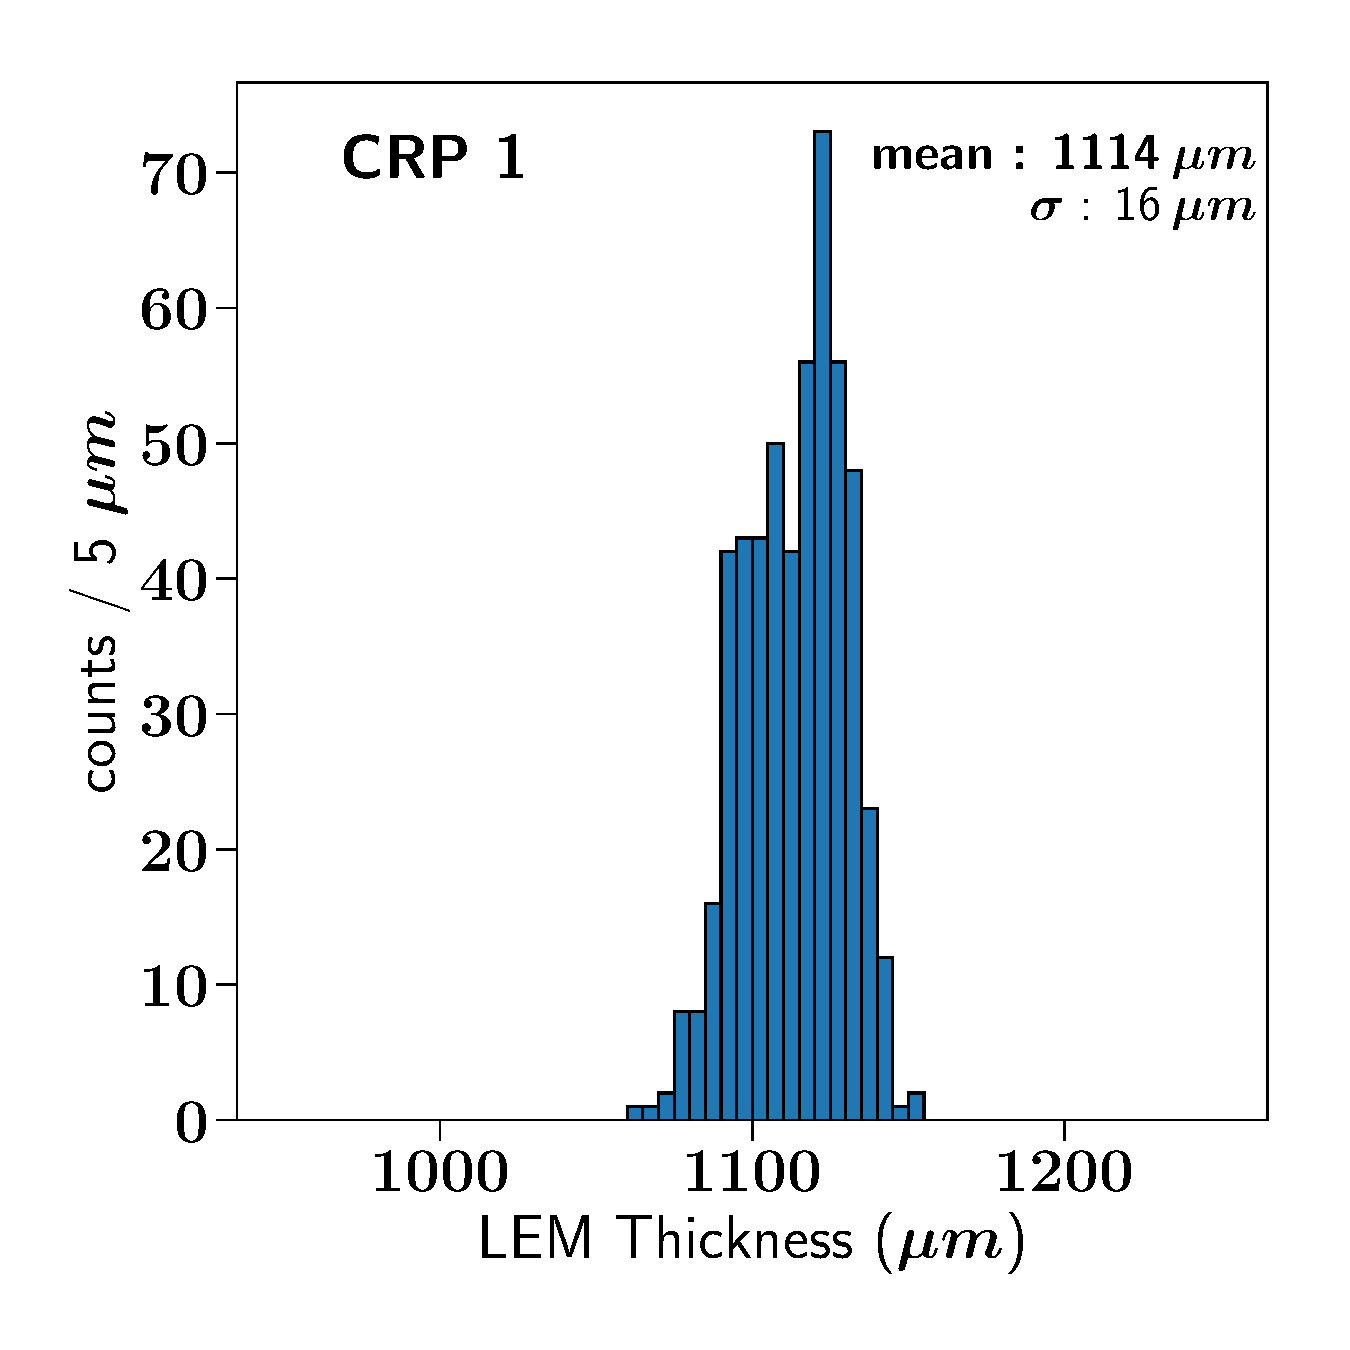
\includegraphics[width=\textwidth,keepaspectratio]{LEM_sum_all_histo_Saclay.pdf}
            \caption{\label{fig::distri_lem_saclay}Distribution de l'épaisseur totale de tous les \glspl{lem} du \gls{crp} 1 du démonstrateur \SSS{} mesurée à travers les 24 trous de la plaque d'acier.}
          \end{subfigure}
          \hfill
          \begin{subfigure}[t]{0.48\textwidth}
            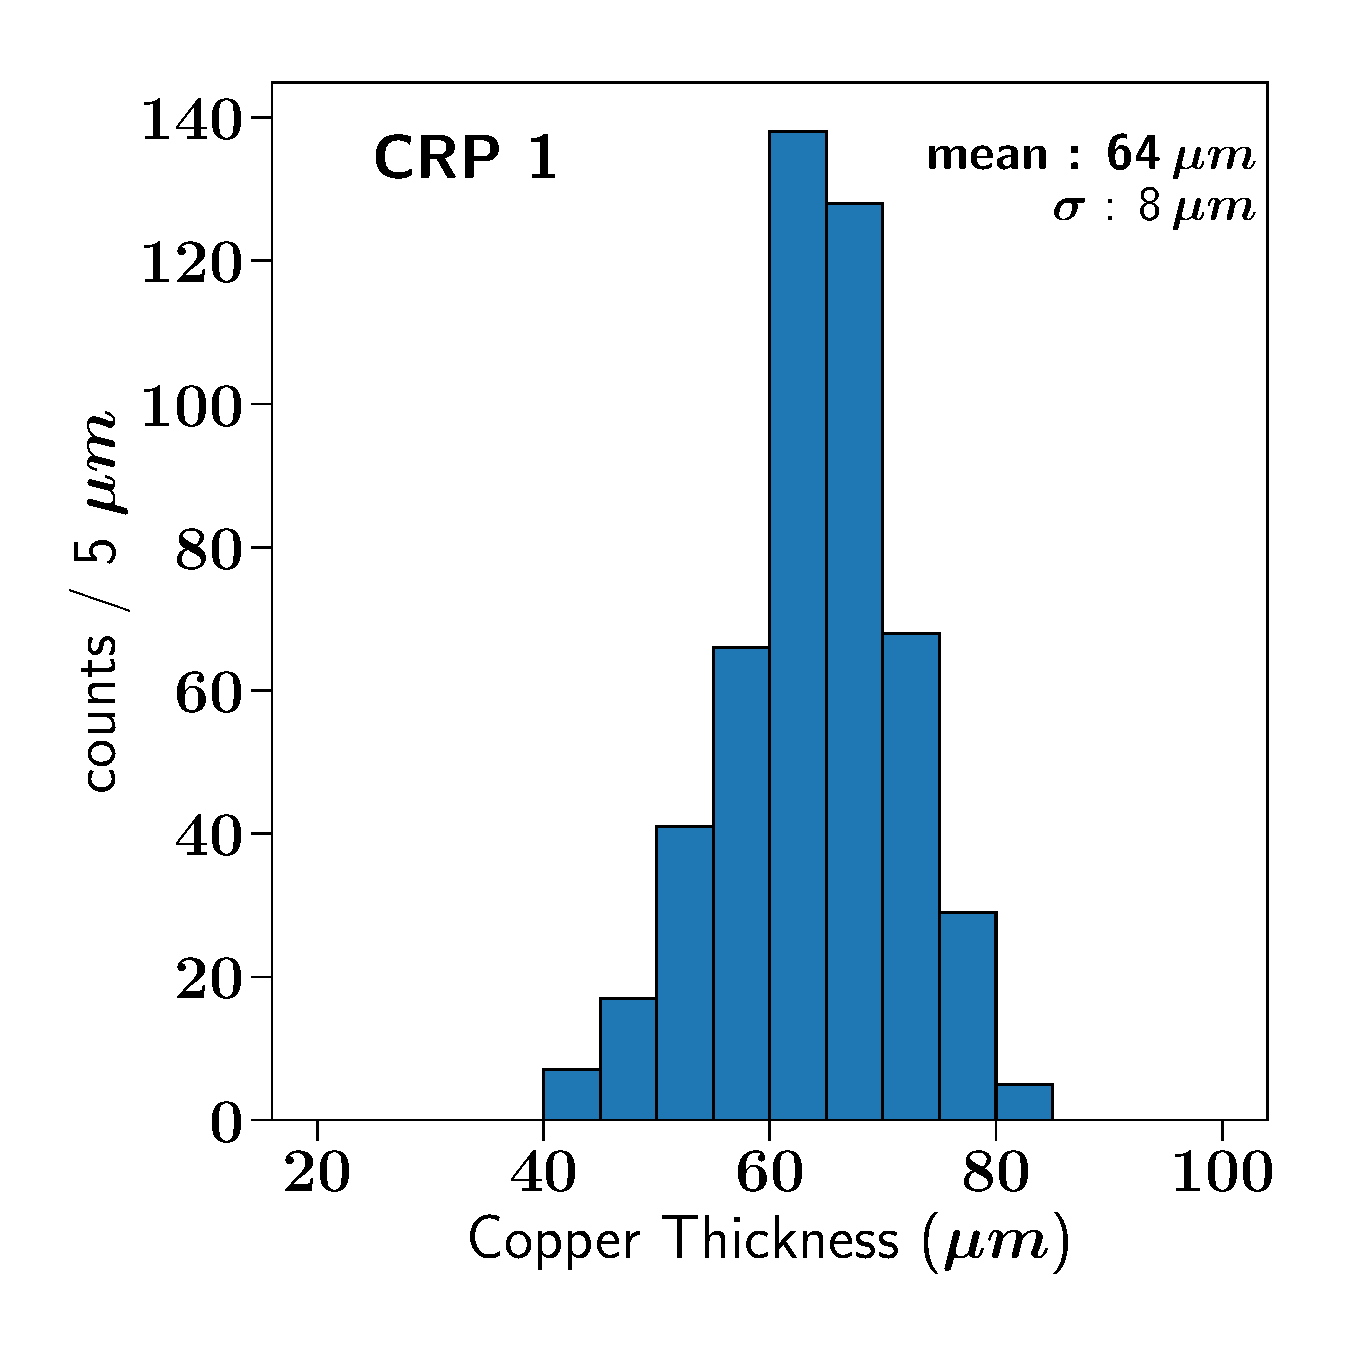
\includegraphics[width=\textwidth,keepaspectratio]{Copper_sum_all_histo_Saclay.pdf}
            \caption{\label{fig::distri_cuivre_saclay}Distribution de l'épaisseur de cuivre de tous les \glspl{lem} du \gls{crp} 1 du démonstrateur \SSS{} mesurée à travers les 24 trous de la plaque d'acier.}
          \end{subfigure}\\
          \begin{subfigure}[b]{0.48\textwidth}
            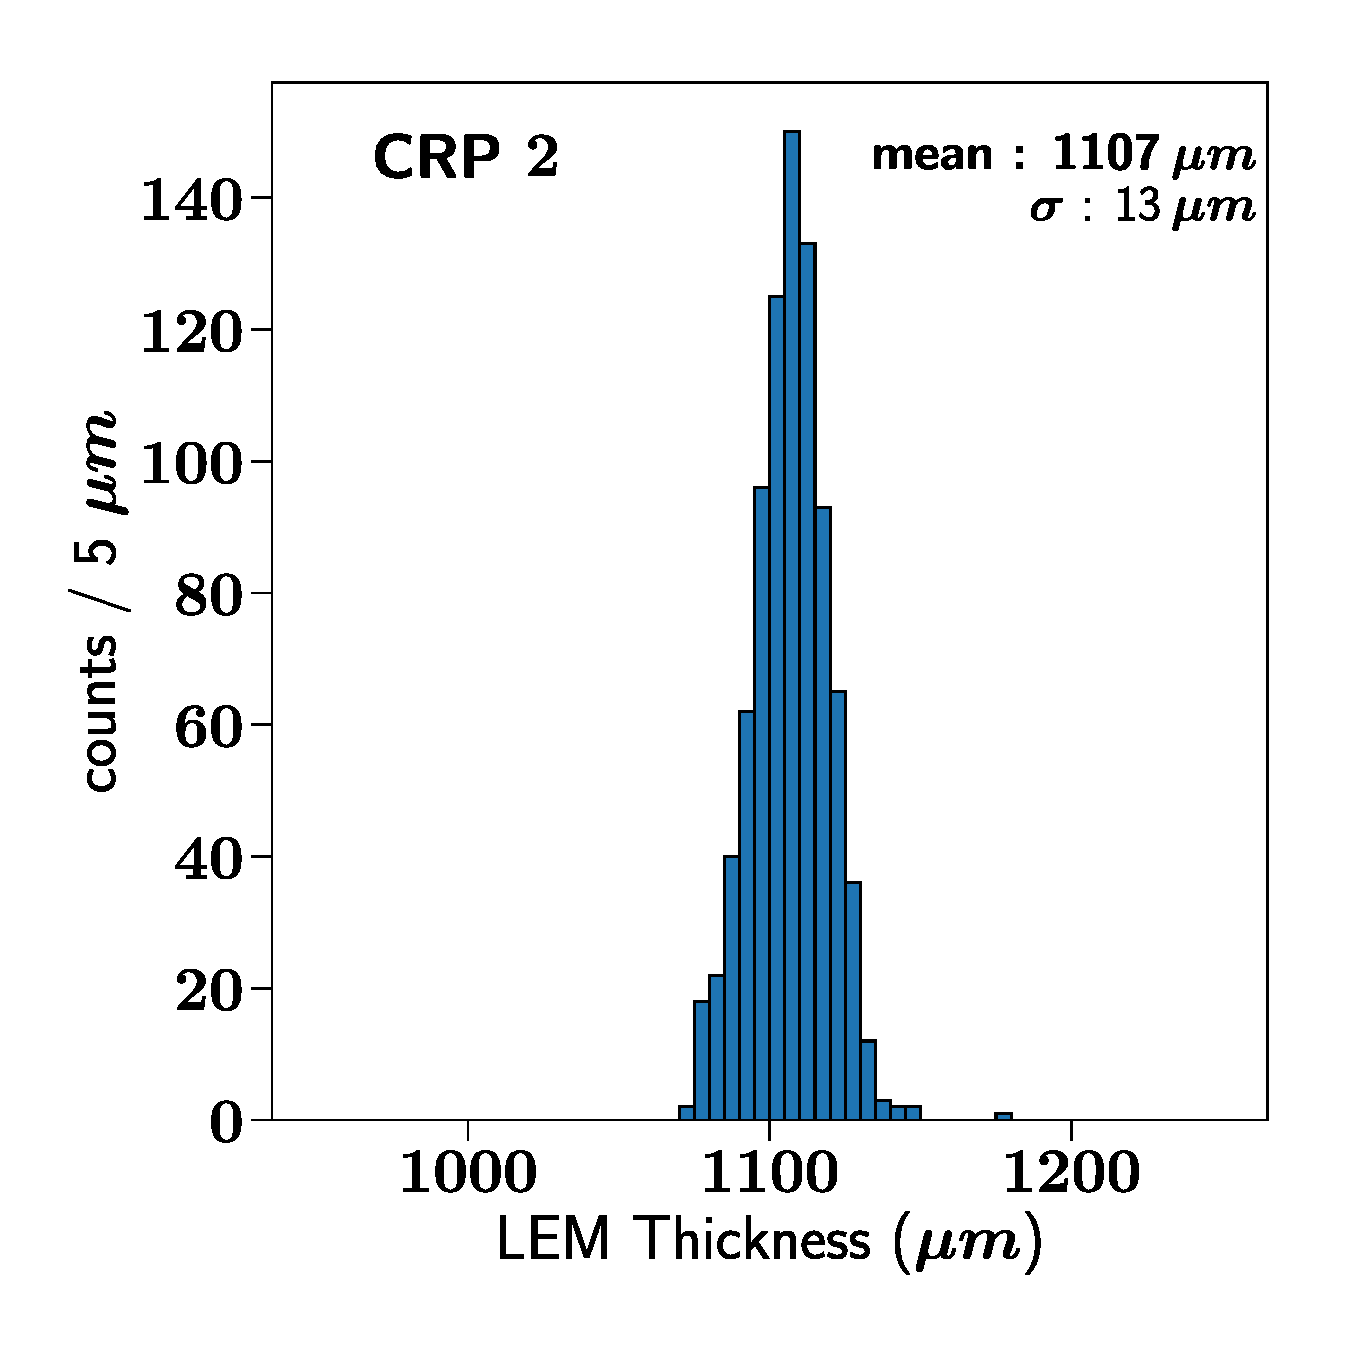
\includegraphics[width=\textwidth,keepaspectratio]{LEM_sum_all_histo_CERN.pdf}
            \caption{\label{fig::distri_lem_cern}Distribution de l'épaisseur totale de tous les \glspl{lem} du \gls{crp} 2 du démonstrateur \SSS{} mesurée à travers les 24 trous de la plaque d'acier.}
          \end{subfigure}
          \hfill
          \begin{subfigure}[b]{0.48\textwidth}
            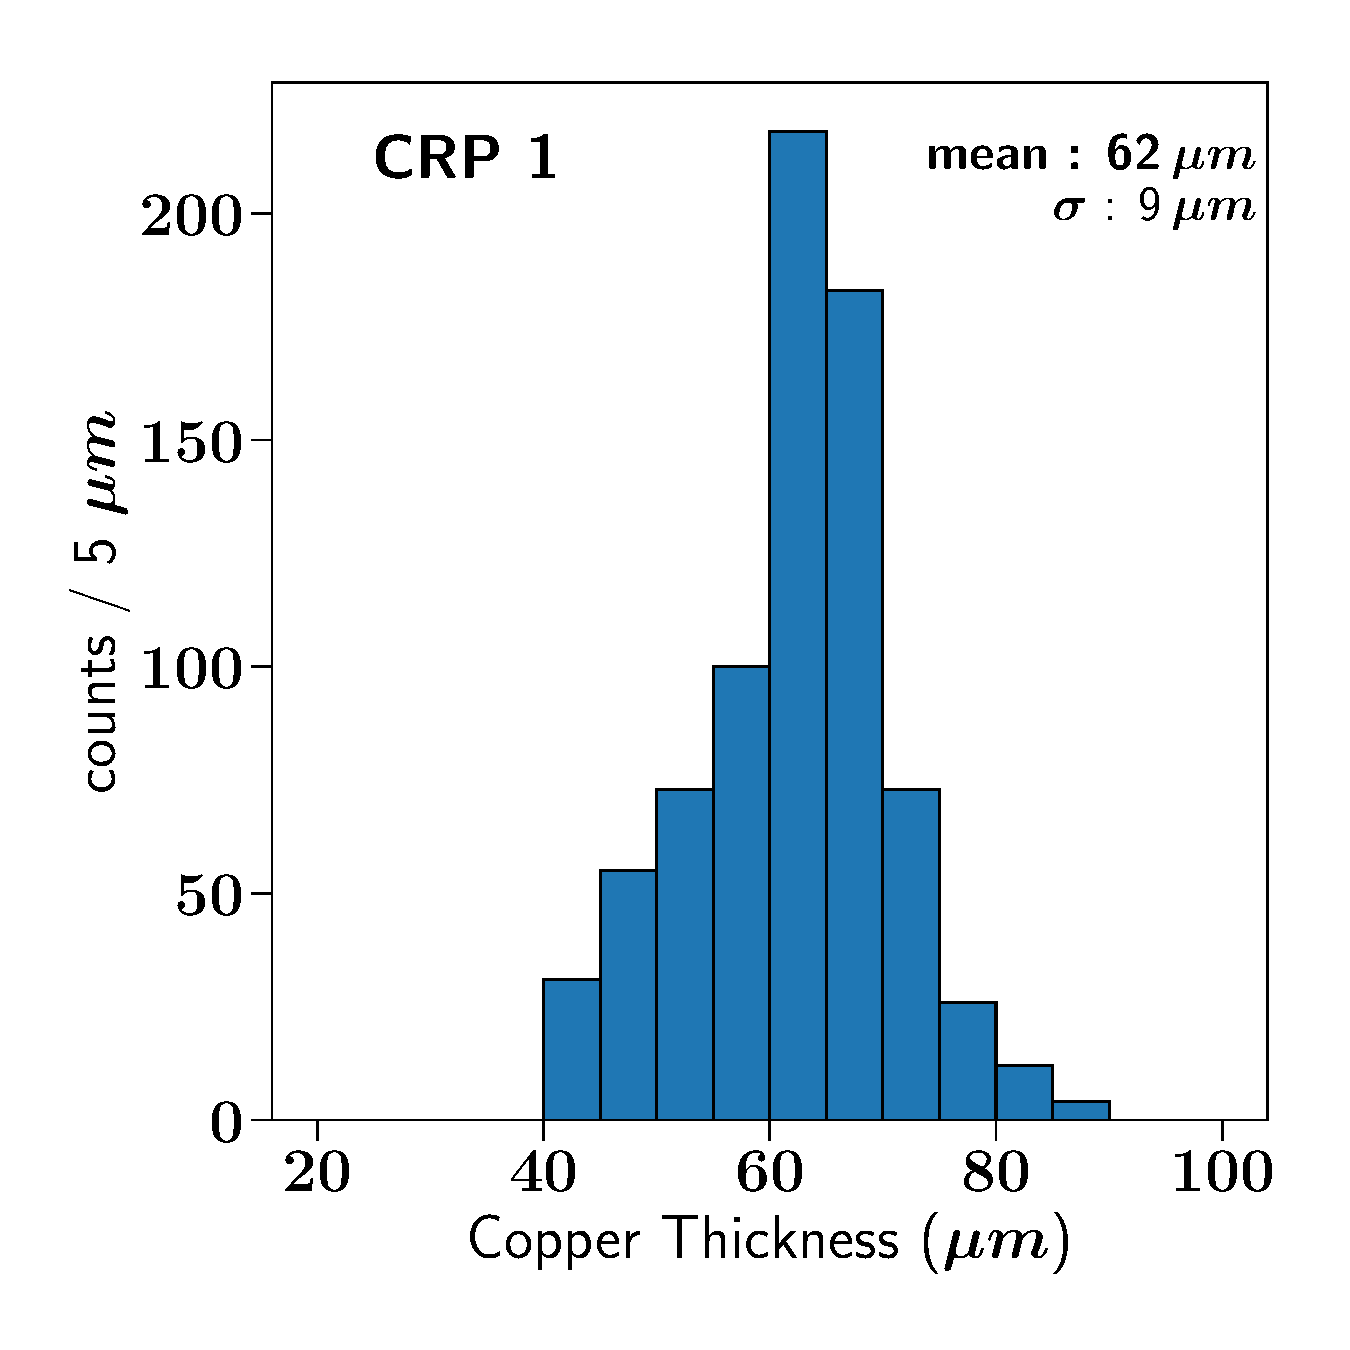
\includegraphics[width=\textwidth,keepaspectratio]{Copper_sum_all_histo_CERN.pdf}
            \caption{\label{fig::distri_cuivre_cern}Distribution de l'épaisseur de cuivre de tous les \glspl{lem} du \gls{crp} 2 du démonstrateur \SSS{} mesurée à travers les 24 trous de la plaque d'acier.}
          \end{subfigure}
          \caption[Résultats des mesures d'épaisseur pour tous les LEM]{\label{fig::epaisseur_tous_lem}Résultats des mesures d'épaisseur pour tous les \glspl{lem}. La première ligne correspond aux \glspl{lem} du \gls{crp} 1 du démonstrateur \SSS{}, la seconde ligne correspond aux \glspl{lem} du \gls{crp} 2 du démonstrateur \SSS{}.}
        \end{figure}
                
%        \begin{figure}[htpb]
%          \begin{subfigure}[t]{0.48\textwidth}
%            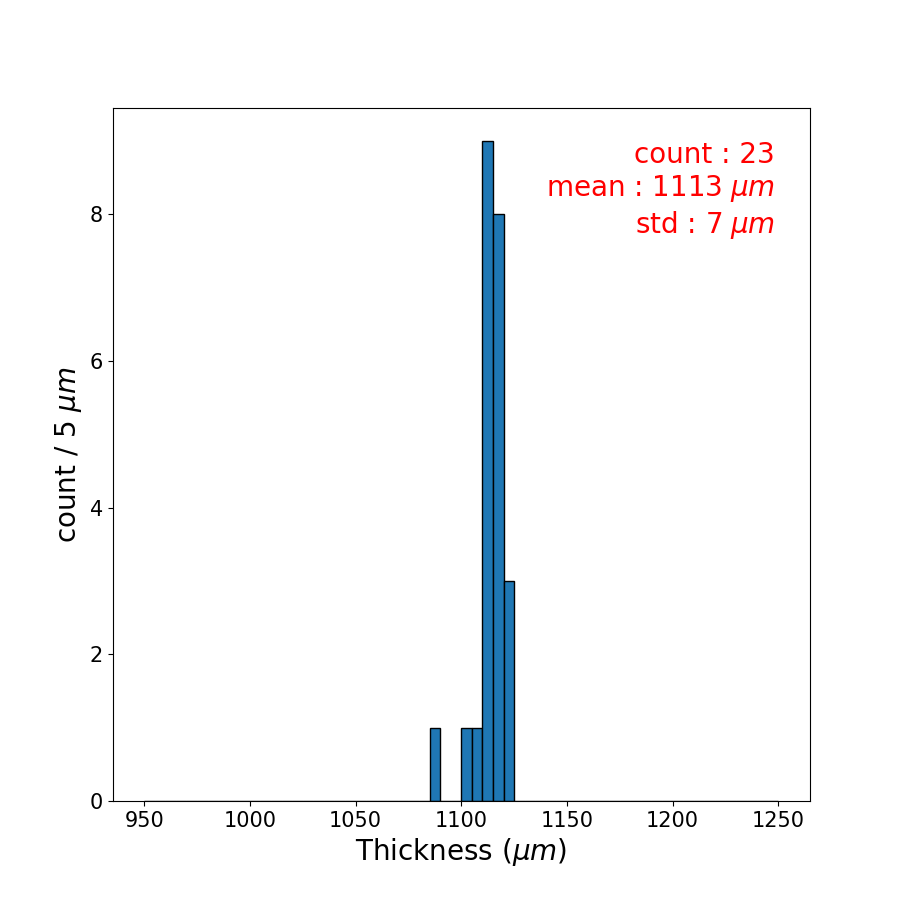
\includegraphics[width=\textwidth,keepaspectratio]{LEM_means_sum_all_histo_saclay.png}
%            \caption{\label{fig::distri_moyenne_lem_saclay}Distribution de l'épaisseur de totale moyennée sur les 24 trous de mesure d'un \gls{lem} pour tous les \glspl{lem} du \gls{crp} 1 du démonstrateur \SSS{}. Seuls \numprint{22} des \numprint{36} \glspl{lem} ont été mesurés.}
%          \end{subfigure}
%          \hfill
%          \begin{subfigure}[t]{0.48\textwidth}
%            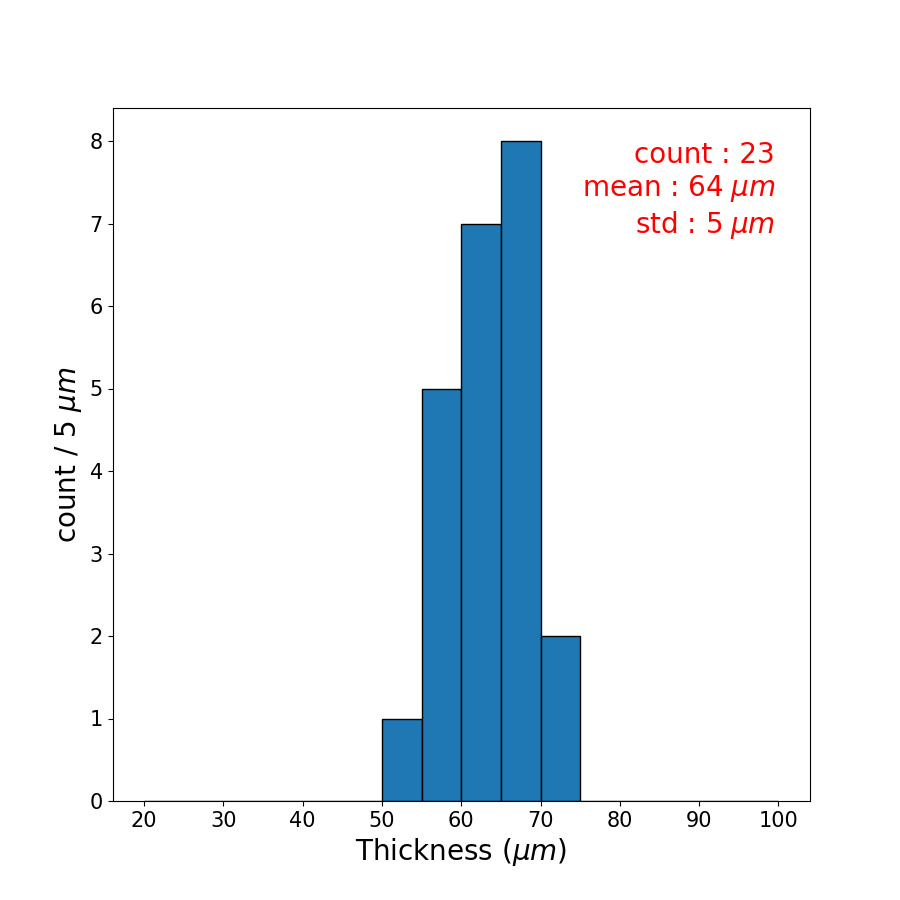
\includegraphics[width=\textwidth,keepaspectratio]{Copper_means_sum_all_histo_saclay.png}
%            \caption{\label{fig::distri_moyenne_cuivre_saclay}Distribution de l'épaisseur de cuivre moyennée sur les 24 trous de mesure d'un \gls{lem} pour tous les \glspl{lem} du \gls{crp} 1 du démonstrateur \SSS{}. Seuls \numprint{22} des \numprint{36} \glspl{lem} ont été mesurés}
%          \end{subfigure}\\
%          \begin{subfigure}[b]{0.48\textwidth}
%            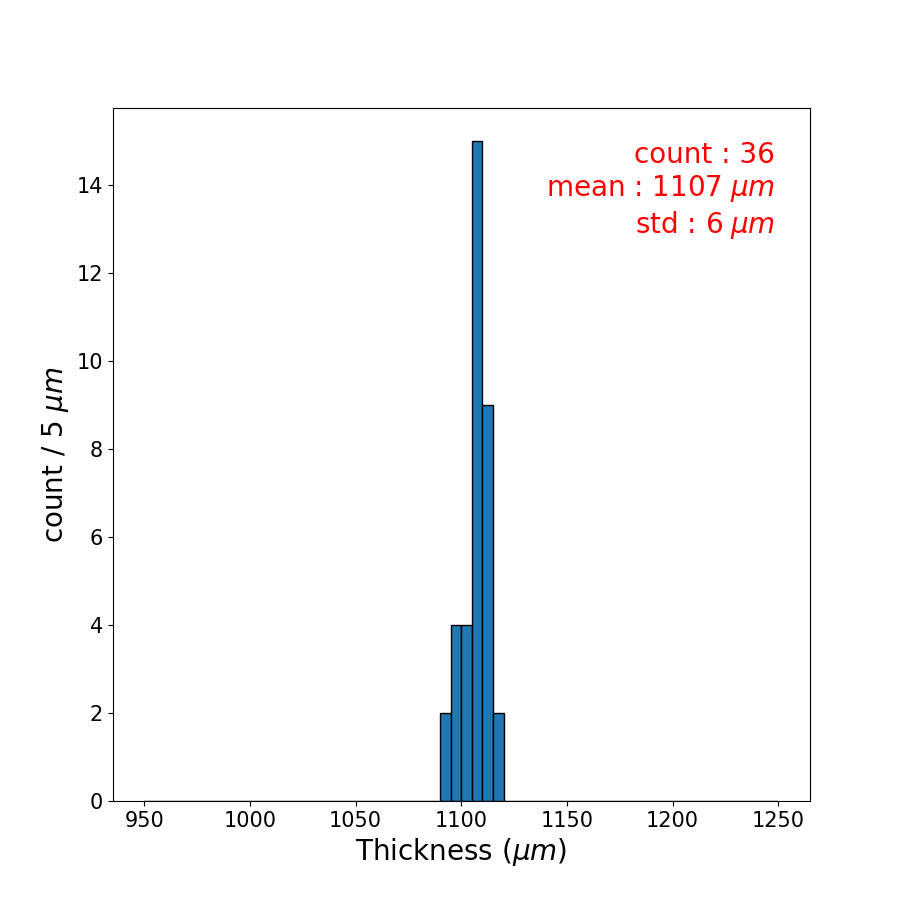
\includegraphics[width=\textwidth,keepaspectratio]{LEM_means_sum_all_histo_cern.png}
%            \caption{\label{fig::distri_moyenne_lem_cern}Distribution de l'épaisseur de totale moyennée sur les 24 trous de mesure d'un \gls{lem} pour tous les \glspl{lem} du \gls{crp} 2 du démonstrateur \SSS{}.}
%          \end{subfigure}
%          \hfill
%          \begin{subfigure}[b]{0.48\textwidth}
%            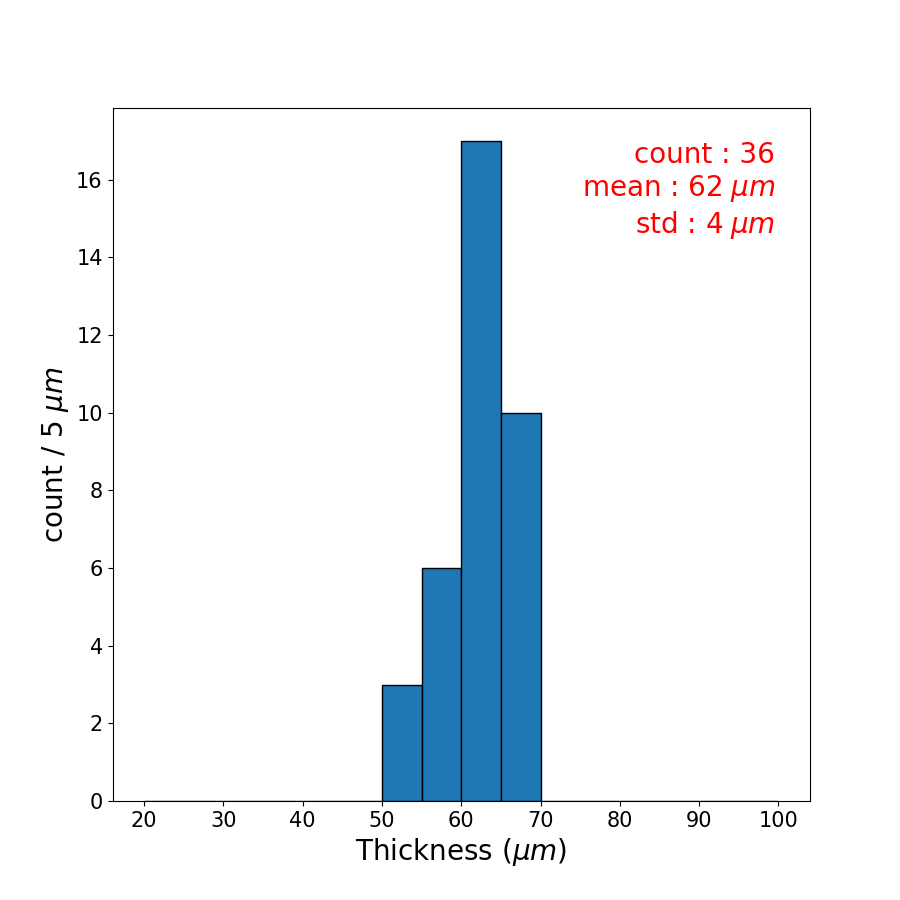
\includegraphics[width=\textwidth,keepaspectratio]{Copper_means_sum_all_histo_cern.png}
%            \caption{\label{fig::distri_moyenne_cuivre_cern}Distribution de l'épaisseur de cuivre moyennée sur les 24 trous de mesure d'un \gls{lem} pour tous les \glspl{lem} du \gls{crp} 2 du démonstrateur \SSS{}.}
%          \end{subfigure}
%          \caption[Résultats des mesures d'épaisseurs moyennées sur les 24 trous de mesure pour tous les \glspl{lem}.]{\label{fig::epaisseur_moyenne_tous_lem}Résultats des mesures d'épaisseur moyennée sur les 24 trous de mesure pour tous les \glspl{lem}. La première ligne correspond aux \glspl{lem} du \gls{crp} 1 du démonstrateur \SSS{}, la seconde ligne correspond aux \glspl{lem} du \gls{crp} 2 du démonstrateur \SSS{}.}
%        \end{figure}
            
        \begin{figure}[htbp]
          \centering
          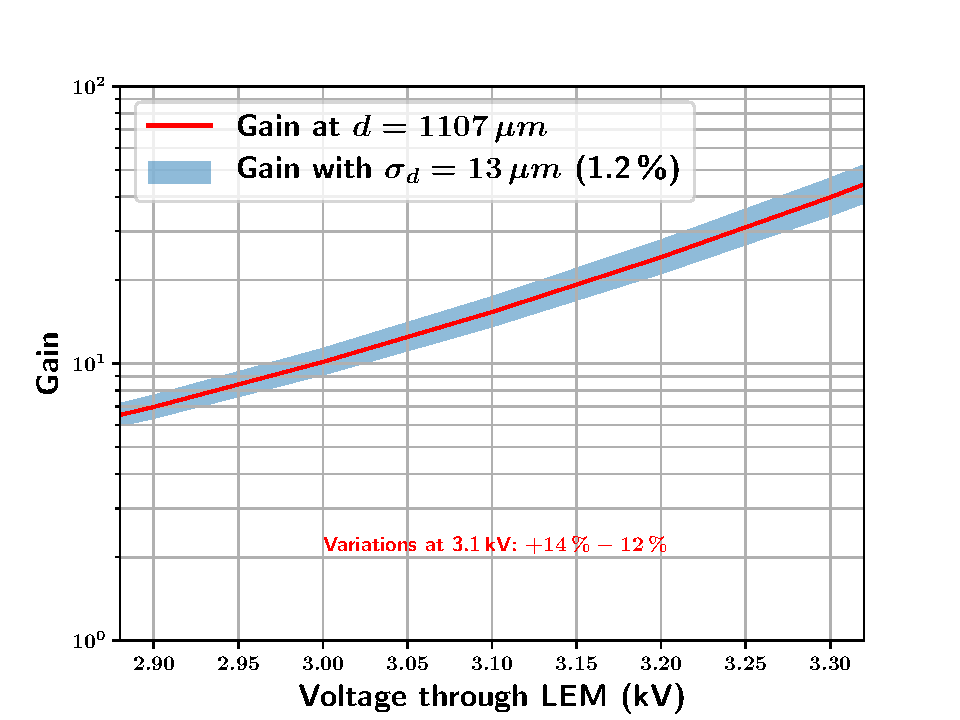
\includegraphics[width=0.8\textwidth,keepaspectratio]{measured_gain_fluctuations}
          \caption[Variation attendues du gain pour l'épaisseur moyennes des \glspl{lem} mesurés]{\label{fig::exp_gain_range}Variation attendue du gain pour une épaisseur de \gls{lem} de $\SI{1107}{\micro\meter}\pm\SI{13}{\micro\meter}$, d'après la formule \eqref{eq::townsend_avalanche_2} ajustée aux données du prototype de \threeL{}\cite{Cantini2014}.}
        \end{figure}
                
        Les distributions des hauteurs dans les 24 trous de mesure d'un \gls{lem} sont tracées avec correction pour la pente du marbre dans la \autoref{fig::distri_1_trou_lem}. Les pics sur les côtés des trous d'amplification étaient attendus, et sont dues une limitation de la technique \gls{cci} : certains rayons lumineux du crayon optique, qui ne sont pas focalisés sur la surface du \gls{fr4} et qui donc ne devraient pas être détectés, sont tout de même réfléchis par la paroi verticale en cuivre et sont détectés par le dispositif, faussant ainsi la distance mesurée. Ces pics, éliminés dans l'analyse, n'affectent pas la mesure de l'épaisseur totale. Les épaisseur de cuivre et de \gls{fr4} en revanche sont estimés à partir des quelques points de mesures pris sur la surface de \gls{fr4} des RIMs. La statistique étant faible sur cette surface il est possible que la mesure de l'épaisseur soit surestimée à cause de l'effet décrit plus haut. Les comparaisons aux mesures d'ELTOS semblent confirmer cette hypothèse, la technique \gls{cci} donnant un résultat plus grand d'environ \SI{10}{\micro\meter}. Cependant, ELTOS ne mesurant ces épaisseurs que sur les bords des \glspl{lem}, il est également possible que l'épaisseur de cuivre ne soit pas identique au milieux et au bord.
                
        Une double gaussienne est ajustée sur la distribution montrée en \autoref{fig::distri_1_trou_lem} afin de déterminer l'épaisseur totale $E_T$ du \gls{lem} ainsi que l'épaisseur $E_C$ du cuivre. La moyenne de la gaussienne la plus à droite sur la \autoref{fig::distri_1_trou_lem} correspond à l'épaisseur totale $E_T$ du \gls{lem}, tandis que la moyenne de la gaussienne la plus à gauche correspond à $E_T - E_C$, en supposant que l'épaisseur du cuivre est la même sur chaque face. $E_C$ est alors calculable facilement, de même que l'épaisseur de \gls{fr4} $E_F$ car nous avons la relation $E_T = E_F + 2E_C$.
                
        A noter que les mesures ne permettaient pas toujours de d'ajuster deux gaussiennes. Dans certains cas, seul l'épaisseur totale était accessible, il y a donc moins de statistiques dans les histogrammes des épaisseurs de cuivre et de \gls{fr4}.
                
        La \autoref{fig::distri_epaisseur_1_lem} montre les distributions de l'épaisseur totale et de l'épaisseur de cuivre pour les 24 trous de mesure d'un \gls{lem}. La \autoref{fig::distri_24_trou_lem_2D} montre l'uniformité de l'épaisseur totale d'un \gls{lem}. La comparaison de cette uniformité entre plusieurs \glspl{lem} permet de voir si des zones semblent toujours être plus hautes ou plus basses. De tels zones n'ont pas été observées.
                
        Afin d'estimer les variations attendues du gain sur les deux \glspl{crp} du démonstrateur \SSS{}, la distribution des épaisseurs dans chaque trou de mesure des \glspl{lem} de chaque \gls{crp} est montrée en \autoref{fig::epaisseur_tous_lem}. La \autoref{fig::exp_gain_range} montre les variations attendues du gain pour une épaisseur de \gls{lem} de $\SI{1107}{\micro\meter}\pm\SI{13}{\micro\meter}$, correspondant 36 \glspl{lem} produits par le \gls{cern} (\gls{crp} 2). À \SI{3.1}{\kilo\volt}, la variation est de l'ordre de $15\%$. On peut de plus remarquer qu'en utilisant les ajustements aux données du prototype de \threeL{}, le gain à \SI{3.1}{\kilo\volt} est inférieur à 20. Ceci est due au fait que l'épaisseur totale des \glspl{lem} est autour de \SI{1107}{\micro\meter}, au lieu des \SI{1080}{\micro\meter} des \glspl{lem} du \threeL{}. À même tension, le champ d'amplification est donc plus faible. Les mesures du \SSS{} vérifieront cette valeur de gain, qui est très sensible au valeurs obtenues pour les coefficients $A$ et $B$ de la formule \eqref{eq::townsend_avalanche_2}.
                
%        La \autoref{fig::epaisseur_moyenne_tous_lem} montre la distributions des épaisseurs totales et des épaisseurs de cuivre moyennées sur les 24 trous de chaque \gls{lem} pour les deux \gls{crp}. Elle permet de comparer nos mesures à celles d'ELTOS, qui ne réalisait que 2 mesures par \gls{lem} pour l'épaisseur de cuivre et 4 pour l'épaisseur totale. 
                
      \subsubsection{Comparaison aux mesures faites par ELTOS}\label{sec::thickness_comparison_eltos}
            
        \begin{figure}[htpb]
          \begin{subfigure}[t]{0.68\textwidth}
            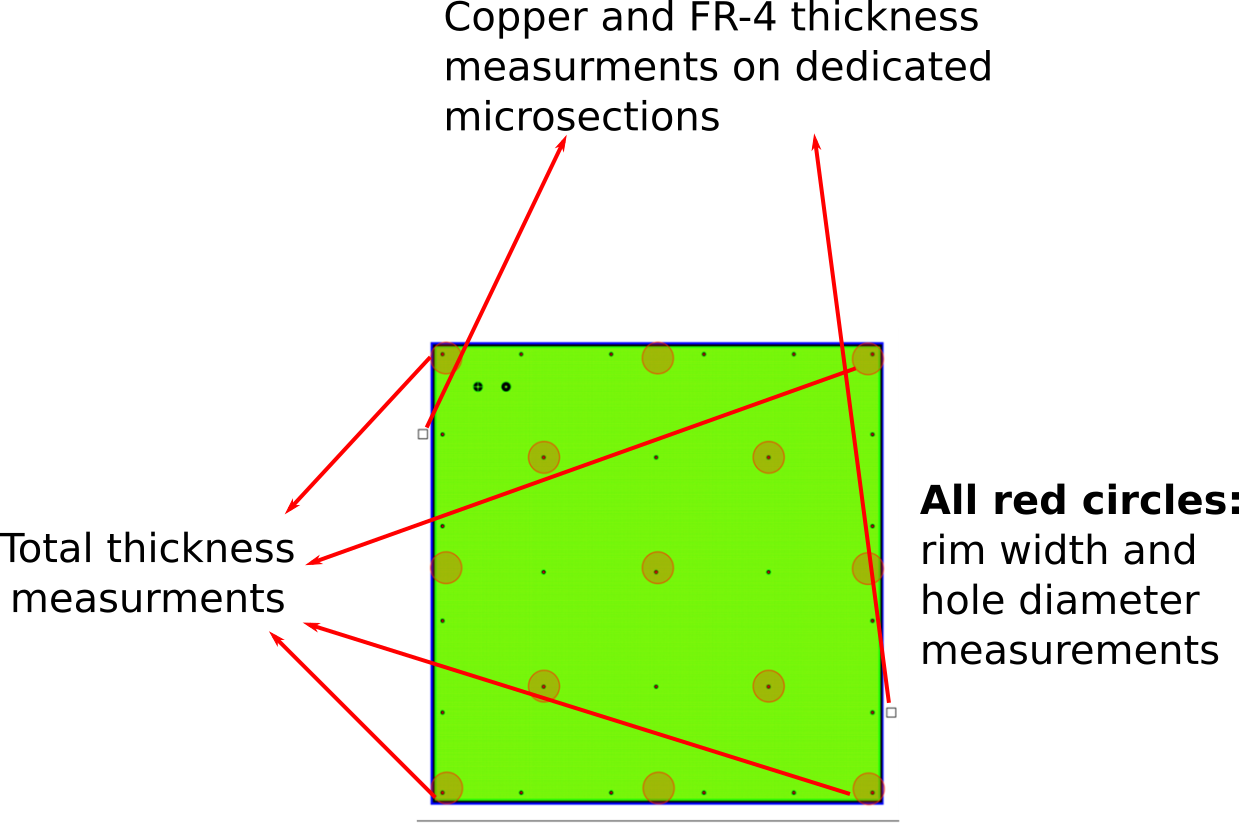
\includegraphics[width=\textwidth]{eltos_measurement.png}
            \caption{Gerber d'un \gls{lem} avec indiquées en rouge les zones de mesure des caractéristiques géométriques pour vérification de la concordance au cahier des charges présenté en \autoref{sec::LEM}. Deux échantillons de surface de \gls{lem} étaient prévues dans le gerber pour y effectuer des mesures d'épaisseur.}
          \end{subfigure}
          \hfill
          \begin{subfigure}[t]{0.3\textwidth}
            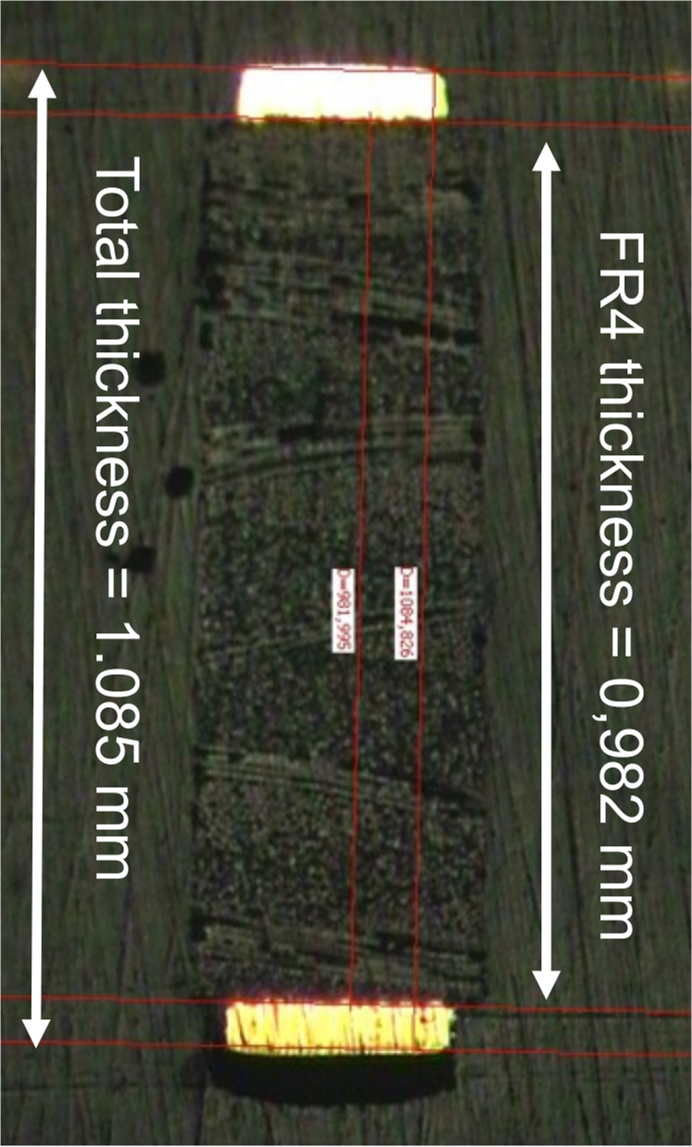
\includegraphics[width=\textwidth]{microsection_thickness.png}
            \caption{\label{fig::microsection}Vue d'un échantillon de surface au microscope où l'on peut voir les mesures d'épaisseur de \gls{fr4} et de cuivre.}
          \end{subfigure}
          \caption[Zones de mesuredes caractéristiques géométriques d'un LEM par ELTOS]{\label{fig::mesures_eltos}zones de mesure des caractéristiques géométriques d'un \gls{lem} par ELTOS}
        \end{figure}
            
        La \autoref{fig::mesures_eltos} montre les zones du \gls{lem} où ELTOS a mesuré les différentes caractéristiques géométriques : la taille totale, l'épaisseur totale, l'épaisseur de cuivre, l'épaisseur de \gls{fr4}, l'épaisseur des RIMs et le diamètre des trous. Les épaisseurs de cuivre et de \gls{fr4} étaient mesurées au microscope sur un des deux échantillons de surface de \gls{lem} prévus dans le gerber à cet effet, donnant une statistique de 72 pour les moyennes et écarts type de chaque \gls{crp} du démonstrateur \SSS{}. L'épaisseur totale était mesurée à 10 microns près avec un micromètre digital, aux quatre coins, donnant une statistique de 144 pour chaque \gls{crp}. L'épaisseur du RIM et le diamètre des trous était mesurés en treize points, donnant une statistique de 468 chacun pour chaque \gls{crp}.
                
%        Due à la faible statistique des épaisseurs de cuivre et des épaisseurs totales, la comparaison aux mesures faites à Saclay est faite avec les distributions des moyennes sur tout le \gls{lem} des mêmes épaisseurs. Le \autoref{tab::mesures_eltos} résume ces résultats et indique ceux obtenus à Saclay.
                
        \begin{table}
          \centering
          \begin{tabular}{l|l|l||l|l|}
            \cline{2-5}
             & \multicolumn{2}{c||}{ELTOS} & \multicolumn{2}{c|}{CCI} \\ \hline
            \multicolumn{1}{|l|}{CRP 1} & \multicolumn{1}{c|}{Moyenne} & \multicolumn{1}{c||}{Écart type} & \multicolumn{1}{c|}{Moyenne} & \multicolumn{1}{c|}{Écart type} \\ \hline
            \multicolumn{1}{|l|}{Épaisseur d'époxy (\gls{fr4})} & \SI{0.97}{\milli\meter} & \SI{10}{\micro\meter} & \SI{1.01}{\milli\meter} & \SI{18}{\micro\meter} \\
            \multicolumn{1}{|l|}{Épaisseur de cuivre} & \SI{45.4}{\micro\meter} & \SI{4.3}{\micro\meter} & \SI{64}{\micro\meter} & \SI{8}{\micro\meter} \\
            \multicolumn{1}{|l|}{Épaisseur Totale} & \SI{1.12}{\milli\meter} & \SI{5}{\micro\meter} & \SI{1.14}{\milli\meter} & \SI{16}{\micro\meter} \\
            \multicolumn{1}{|l|}{Largeur du RIM (haut)} & \SI{41}{\micro\meter} & \SI{1.6}{\micro\meter} &  &  \\
            \multicolumn{1}{|l|}{Largeur du RIM (bas)} & \SI{41}{\micro\meter} & \SI{1.6}{\micro\meter} &  &  \\
            \multicolumn{1}{|l|}{Surface Totale} & \numprint{499.43}$\times$\SI{499.43}{\milli\meter\squared} & \SI{30}{\micro\meter} &  &  \\
            \multicolumn{1}{|l|}{Diamètre des trous} & \SI{500}{\micro\meter} & \SI{1}{\micro\meter} &  &  \\ \hline \hline
            \multicolumn{1}{|l|}{CRP 2} & \multicolumn{1}{c|}{Moyenne} & \multicolumn{1}{c||}{Écart type} & \multicolumn{1}{c|}{Moyenne} & \multicolumn{1}{c|}{Écart type} \\ \hline 
            \multicolumn{1}{|l|}{Épaisseur d'époxy (\gls{fr4})} & \SI{0.97}{\milli\meter} & \SI{10}{\micro\meter} & \SI{0.98}{\milli\meter} & \SI{16}{\micro\meter} \\
            \multicolumn{1}{|l|}{Épaisseur de cuivre} & \SI{46.5}{\micro\meter} & \SI{4.9}{\micro\meter} & \SI{62}{\micro\meter} & \SI{9}{\micro\meter} \\
            \multicolumn{1}{|l|}{Épaisseur Totale} & \SI{1.12}{\milli\meter} & \SI{5}{\micro\meter} & \SI{1.107}{\milli\meter} & \SI{13}{\micro\meter} \\
            \multicolumn{1}{|l|}{Largeur du RIM (haut)} & \SI{41}{\micro\meter} & \SI{1.6}{\micro\meter} &  &  \\
            \multicolumn{1}{|l|}{Largeur du RIM (bas)} & \SI{41}{\micro\meter} & \SI{1.6}{\micro\meter} &  &  \\
            \multicolumn{1}{|l|}{Surface Totale} & \numprint{499.43}$\times$\SI{499.43}{\milli\meter\squared} & \SI{30}{\micro\meter} &  &  \\
            \multicolumn{1}{|l|}{Diamètre des trous} & \SI{500}{\micro\meter} & \SI{1}{\micro\meter} &  &  \\ \hline
            \end{tabular}
          \caption[Mesures des différentes caractéristiques géométriques des LEM]{\label{tab::mesures_eltos}Mesures des différentes caractéristiques géométriques des \glspl{lem} faites par ELTOS les deux \gls{crp} du démonstrateur \SSS{}, et comparaison aux mesures faites à Saclay avec la technique \gls{cci}.}
        \end{table}
            
        Les mesures réalisées par ELTOS et les mesures réalisées par le \gls{cea} sont compatibles pour les épaisseurs totales, mais il y a une différence notable concernant les mesures des moyennes des épaisseurs de cuivre et de \gls{fr4}, bien que les écarts type soient compatibles. En regardant attentivement la \autoref{fig::microsection}, on se rend compte que la mesure du cuivre faite par ELTOS est sous-estimée d'environ $10-$\SI{12}{\micro\meter}. La même observation a été faite sur d'autres échantillons, ce qui ramène les valeurs d'épaisseur de cuivre d'ELTOS indiquées dans le \autoref{tab::mesures_eltos} à des valeurs entre \SI{55}{\micro\meter} et \SI{57}{\micro\meter}. La différence restante avec les mesures faites avec la technique \gls{cci} peut être due à la limitation expliquée en \autoref{sec::thickness_result}.
            
        La technique \gls{cci} se montre efficace pour mesurer l'épaisseur totale des \glspl{lem}. Bien que le dispositif utilisé ici soit lent (minimum trente minutes pour mesurer un \gls{lem}), il pourra être motorisé et automatisé pour une future production à l'échelle de \gls{dune}. Avec une motorisation et une vitesse de déplacement du crayon optique constante et très lente, il pourra être possible de mesurer les RIMs et les diamètres des trous.
        
    \subsection{Tests haute tension dans une enceinte haute pression}\label{sec::test_HT}
        
      \begin{figure}[htpb]
        \begin{subfigure}[t]{0.48\textwidth}
          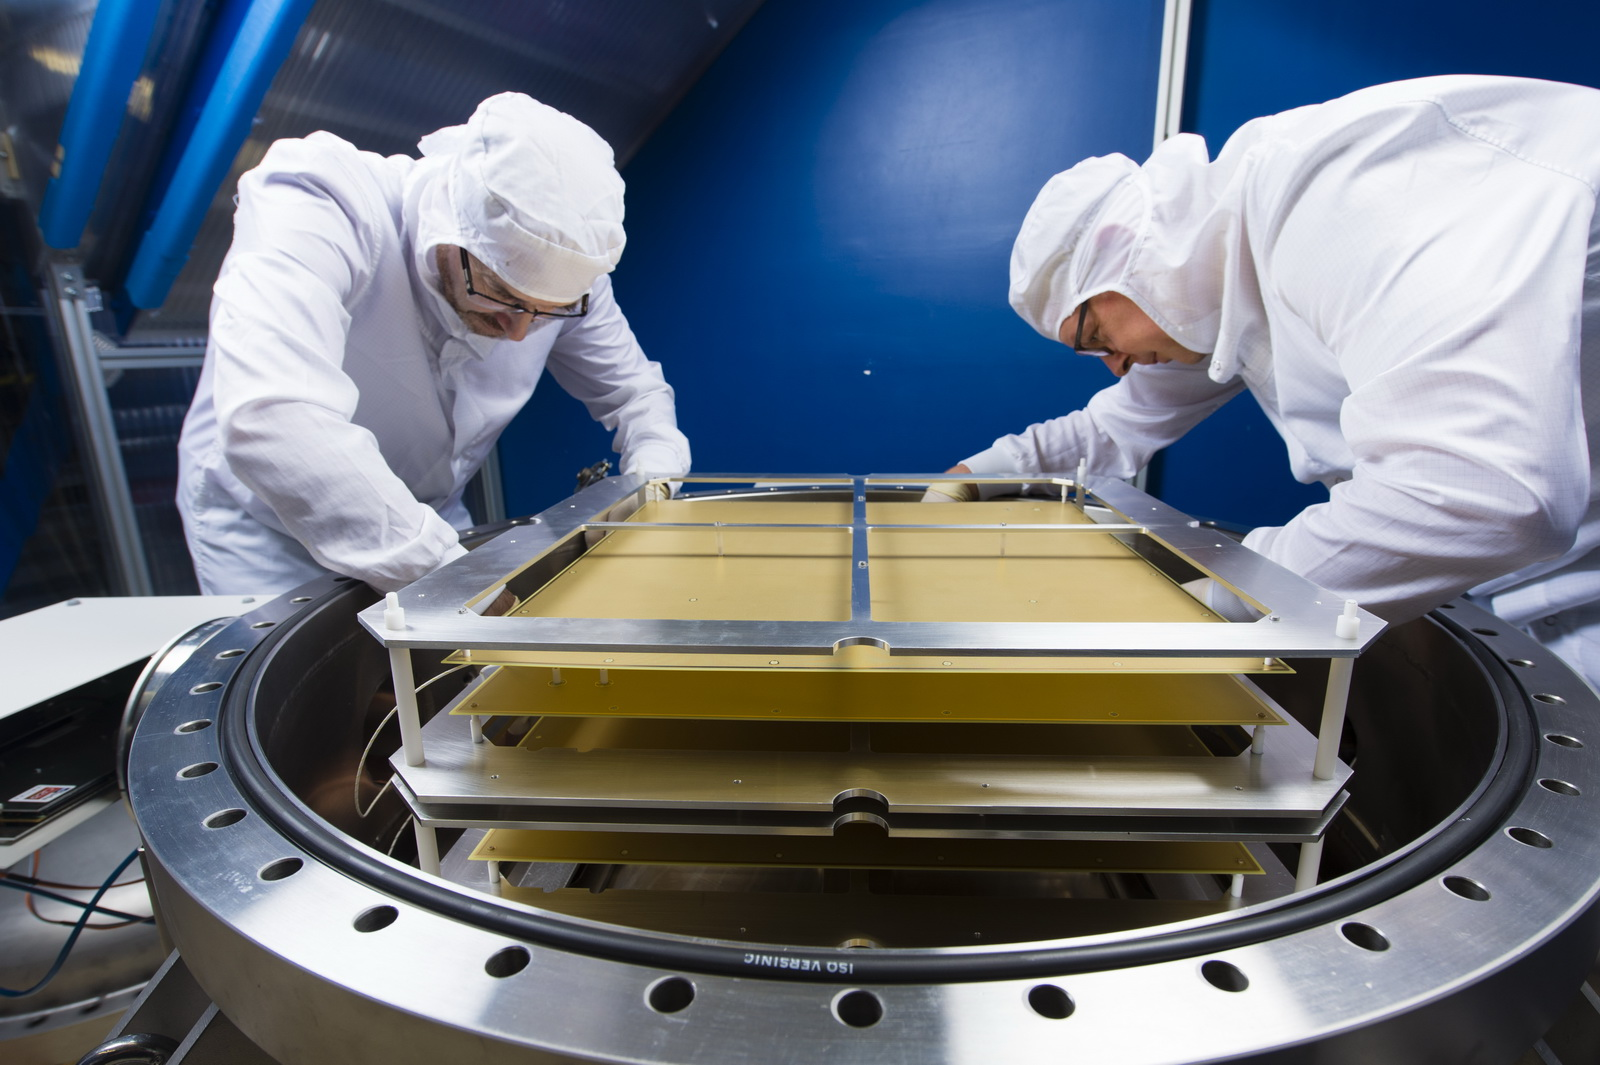
\includegraphics[width=\textwidth,keepaspectratio]{6lems_gamelle.jpg}
          \caption{\label{fig::6lems_gamelle}Enceinte haute pression avec neuf \glspl{lem} en train d'être préparés pour un test de tenue en tension.}
        \end{subfigure}
        \hfill
        \begin{subfigure}[t]{0.48\textwidth}
          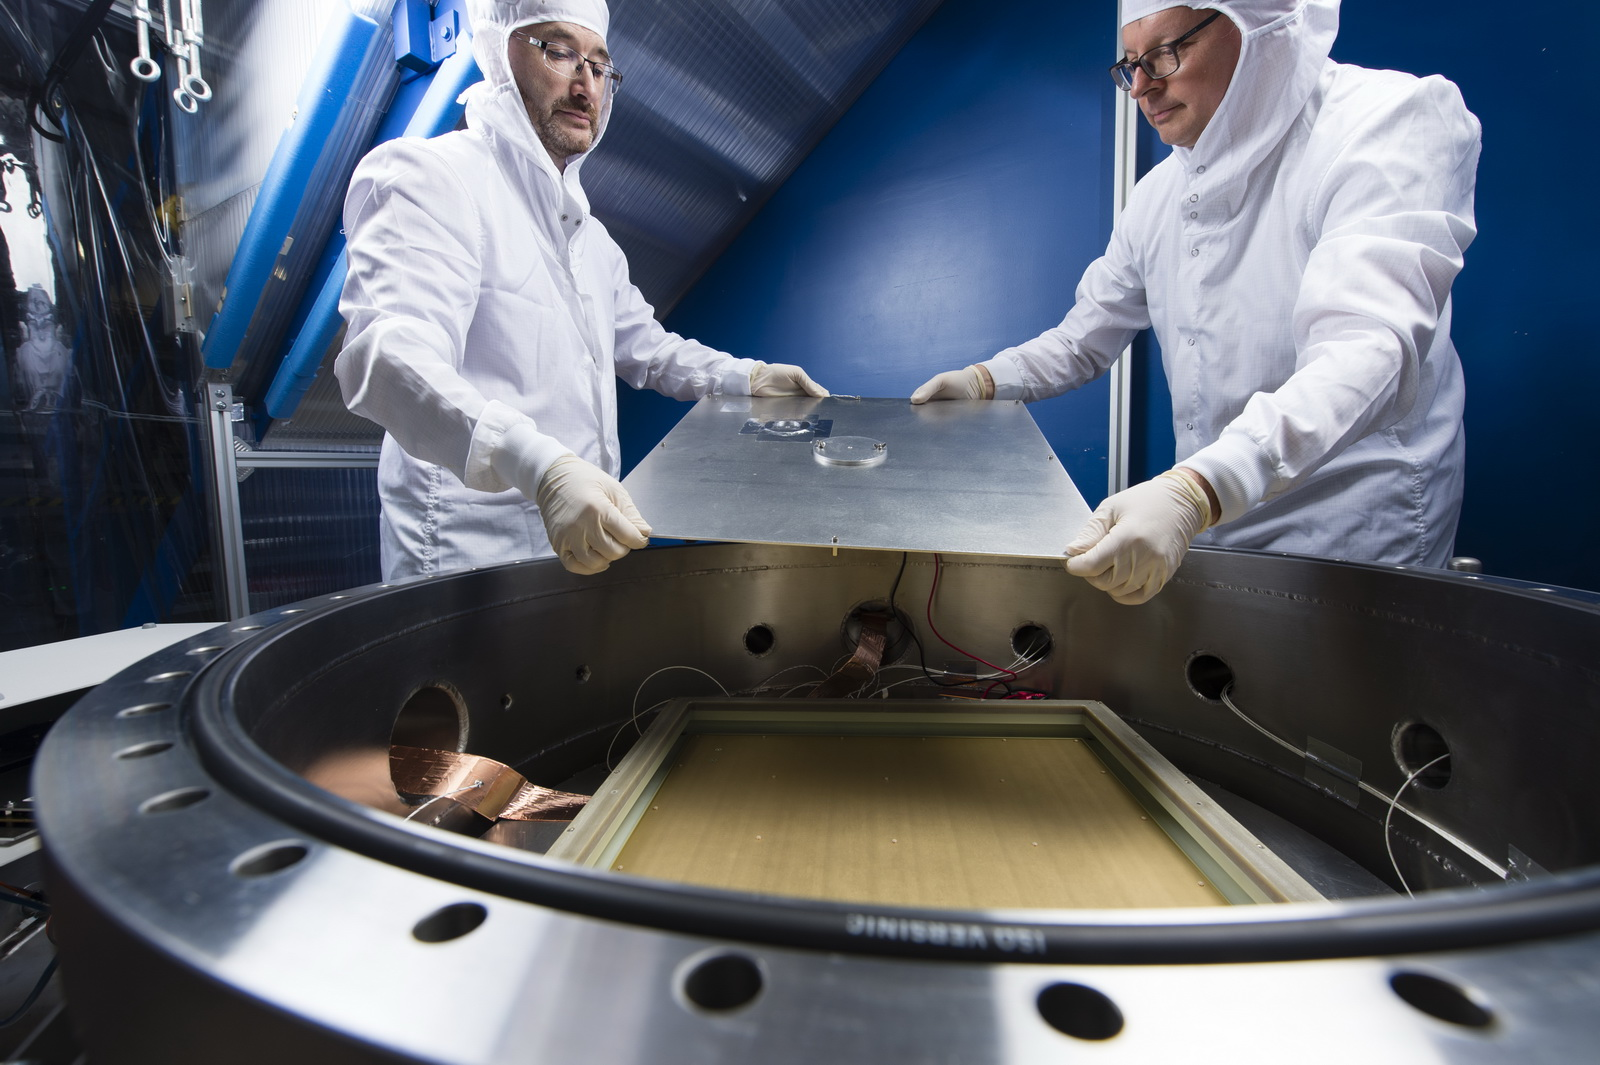
\includegraphics[width=\textwidth,keepaspectratio]{gamelle_source.jpg}
          \caption{\label{fig::gamelle_source}Enceinte haute pression avec une source d'américium, un \gls{lem} et une anode en train d'être préparés pour une mesure de gain.}
        \end{subfigure}
        \caption[Enceinte haute pression]{\label{fig::gamelle}Enceinte haute pression utilisée à Saclay pour les tests de tenue en tension et les mesures de gain des \glspl{lem} destinés au démonstrateur \SSS{}.}
      \end{figure}

      \begin{figure}[htpb]
        \begin{subfigure}[t]{0.48\textwidth}
          \centering
          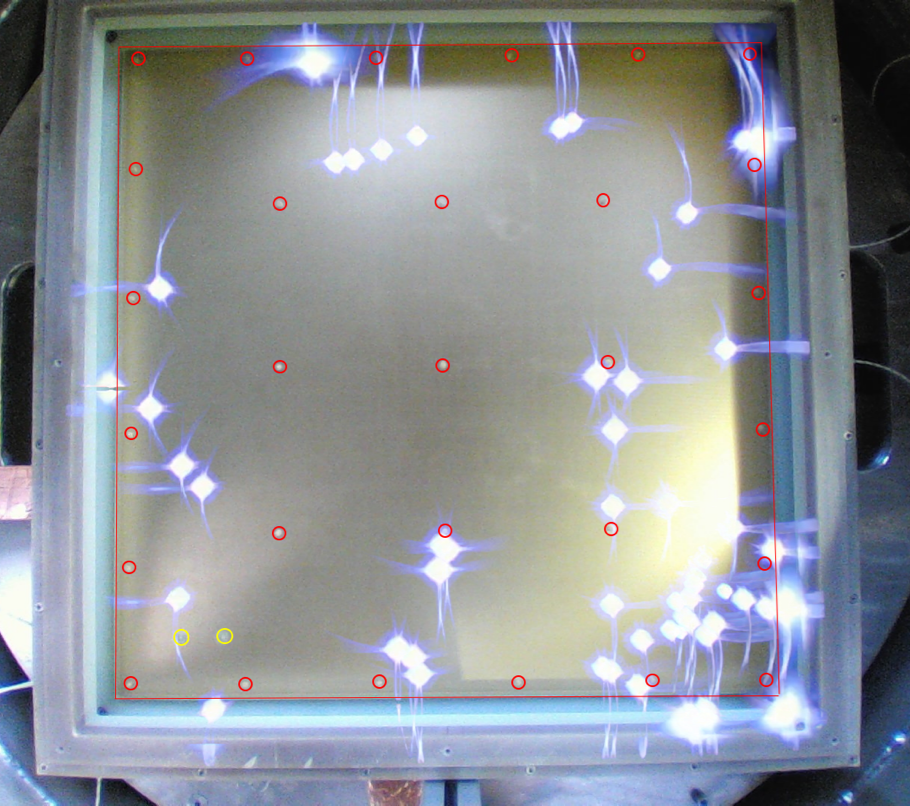
\includegraphics[width=0.8\textwidth,keepaspectratio]{sparks_34.png}
          \caption{\label{fig::sparks_34}Visualisation des décharges sur un \gls{lem} du modèle CFR-34 entre \SI{3.3}{\kilo\volt} et \SI{3.5}{\kilo\volt}. Le taux de décharge est d'environ \SI{20}{\per\hour}.}
        \end{subfigure}
        \hfill
        \begin{subfigure}[t]{0.48\textwidth}
          \centering
          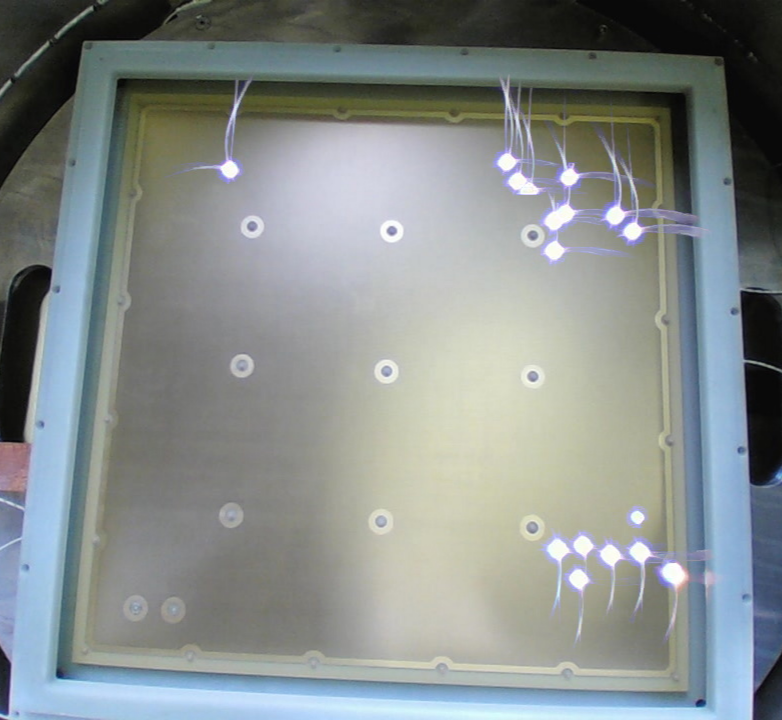
\includegraphics[width=0.8\textwidth,keepaspectratio]{sparks_35.png}
          \caption{\label{fig::sparks_35}Visualisation des décharges sur un \gls{lem} du modèle CFR-35 à \SI{3.5}{\kilo\volt}. Le taux de décharge est d'environ \SI{3}{\per\hour}.}
        \end{subfigure}
        \caption[Visualisation des décharges sur les deux modèles de LEM]{\label{fig::sparks}Visualisation des décharges sur les deux modèles de \gls{lem}.}
      \end{figure}

      Une enceinte haute pression a été construite afin d'y recréer la densité de l'argon gazeux des \glspl{dlartpc} de \gls{wa105}. Tous les \glspl{lem} du démonstrateur \SSS{} y ont été soumis à de hautes tensions afin de déterminer leur tension de claquage, et ce dans de l'air sec ainsi que dans l'argon. A également été mesuré le gain de quelques \glspl{lem} du \SSS{} grâce à une source d'américium placée dans l'enceinte.
            
      Pour les tests haute tension, neuf \glspl{lem} pouvaient être testés en même temps dans l'enceinte. La \autoref{fig::6lems_gamelle} montre  ce dispositif. Pour les mesures de gains, un seul \gls{lem} était placé, ainsi qu'une anode de lecture et la source. L'espacement entre l'anode et le \gls{lem} est le même que sur le \gls{crp}, $\SI{2}{\milli\meter}$. La cathode avec la source est située $\SI{5}{\centi\meter}$ au dessus du \gls{lem}. La \autoref{fig::gamelle_source} montre ce dispositif. Ces tests ont permis de mettre en évidence une limitation des \glspl{lem} du modèle CFR-34, utilisé dans le prototype de \TOO{}. Ces derniers présentaient un taux de claquage bien trop grand (autour de 20 par heure) au delà de \SI{3.3}{\kilo\volt}. La tension voulue étant de \SI{3.1}{\kilo\volt}, cela laissait trop peu de marge d'erreur. Comme les décharges semblaient avoir lieu essentiellement sur les bords (voir \autoref{fig::sparks}), un modèle avec des zones mortes plus grandes a été mis au point, le CFR-35, décrit en \autoref{sec::LEM}. Ce modèle présente alors un taux de claquage autour de 3 par heure à \SI{3.5}{\kilo\volt} et a été retenu pour le \SSS{}. Une étude visant à déterminer la dimension optimale des bords afin de limiter les claquages tout en conservant une zone active raisonnable est en cours avec le logiciel COMSOL Multiphysics.

    \subsection{Mesures de gain dans une enceinte haute pression}\label{sec::test_gain}

      \begin{figure}[htpb]
        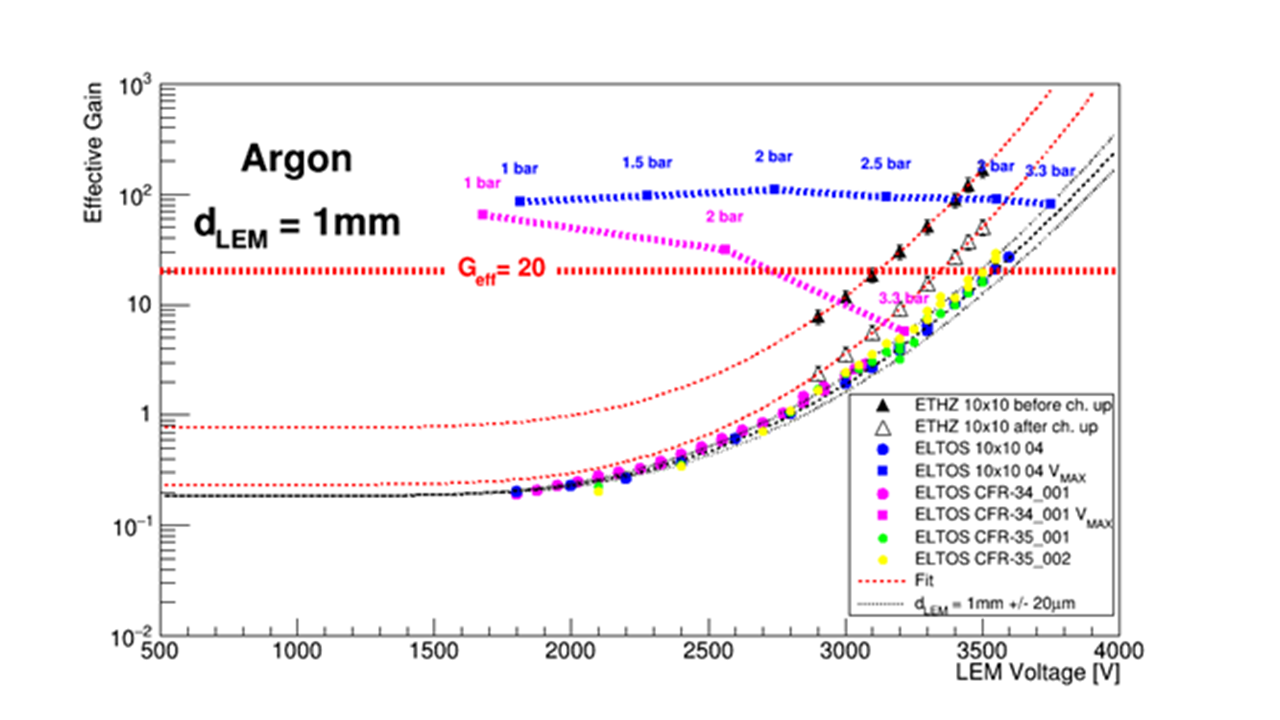
\includegraphics[width=\textwidth,keepaspectratio]{gain_2.png}
        \caption[Mesure du gain dans l'enceinte haute pression]{\label{fig::gain_gamelle}Mesure du gain dans l'enceinte haute pression pour plusieurs modèles de \glspl{lem} (ronds et carrés). Les triangles pleins sont les mesures avant charging up faites par le prototype de \threeL{}\cite{Cantini2014}, les triangles vides sont les gains attendus du \threeL{} après charging up (voir texte).}
      \end{figure}

      Des mesures de gain ont été faites dans l'enceinte haute pression pour plusieurs \glspl{lem} : des prototypes de $10\times\SI{10}{\centi\meter\squared}$, semblables à ceux utilisés dans le prototype de \threeL{}, ainsi que des \glspl{lem} de $50\times\SI{50}{\centi\meter\squared}$ CFR-34 et CFR-35. Plusieurs pressions ont été utilisées, allant de 1 à \SI{3.3}{\bar}, équivalent à la densité de l'argon gazeux des \glspl{dlartpc} de \gls{wa105}. Toutes ces mesures sont faites après charging up complet du \gls{lem}.

      La \autoref{fig::gain_gamelle} montre le résultat de ces mesures. Tous les \glspl{lem} testés dans l'enceinte ont un comportement identiques. Sur cette même figure sont également représentées les données du prototype de \threeL{} issues de \cite{Cantini2014} avant charging up. Un facteur de \numprint{2.7} a été utilisé pour estimer le gain après charging up de ces mêmes données, correspondant au ratio avant/après charging up mesuré dans le \threeL{} à \SI{3.4}{\kilo\volt}. On peut constater que les mesures réalisées dans l'enceinte haute pression sont inférieure au gain attendu après charging up d'après le \threeL{}. Cette différence n'est pas encore bien comprises, et une calibration précise du gain va être réalisée en effectuant des mesures avec et sans \gls{lem}. 

      Sur la même figure sont également représentés les gains maximums attendus dans l'enceinte à différentes pressions. Ces valeurs sont obtenue en mesurant la tension maximale supportée par les \glspl{lem} à ces pressions. Le gain maximum est ensuite estimé à partir de l'ajustement de l'équation \eqref{eq::gain_eff} aux gains mesurés à ces même pressions à des tensions plus basses. On constate que les \glspl{lem} de $50\times\SI{50}{\centi\meter\squared}$  CFR-34 atteignent des tensions plus faibles que ceux de $10\times\SI{10}{\centi\meter\squared}$.
        
    \subsection{Test de continuité des canaux de lecture des anodes}\label{sec::test_anode}

      \begin{figure}
        \begin{subfigure}[t]{0.48\textwidth}
          \includegraphics[width=\textwidth,keepaspectratio]{anode_card_zoom.png}
          \caption{\label{fig::anode_card_zoom}Agrandissement d'une carte de mesure. On y voit les résistances de \SI{100}{\ohm} placées entre les canaux de l'anode.}
        \end{subfigure}
        \hfill
        \begin{subfigure}[t]{0.48\textwidth}
          \includegraphics[width=\textwidth,keepaspectratio]{anode_carde.png}
          \caption{\label{fig::anode_card}Photo du dispositif de mesure. Les cartes de chaque côtés permettent aux \numprint{160} canaux de l'anode de n'en former plus qu'un, si aucun n'est cassé. Les cartes au dessus et en dessous servent à vérifier qu'il n'y a pas de court circuit entre les deux vues de l'anode.}
        \end{subfigure}
        \caption[Dispositif de mesure de la continuité des canaux de lecture des anodes]{\label{fig::test_anode}Dispositif de mesure de la continuité des canaux des lecture des anodes.}
      \end{figure}
      La continuité des canaux de lecture des anodes ainsi que leur isolation les uns par rapport aux autres ont été testées grâce à des \glspl{pcb} créés à cet effet. Deux jeux de deux cartes de test ont été produits et ont permis de valider les 72 anodes du démonstrateur \SSS{} et les 6 anodes de rechange.
      
      Ces cartes sont munies des mêmes connecteurs que les anodes. Elles sont faites de manière à ce qu'en branchant une carte de chaque côté de l'anode, les 160 canaux d'une vue de l'anode forment un circuit continue. Des zones de cuivres sont prévus entre chaque groupe de 32 canaux afin d'y mesurer la résistance du groupe. La \autoref{fig::test_anode} montre le dispositif de mesure.

      Entre chaque canal est insérée une résistance de $\SI{100}{\ohm}$. Ainsi, une résistance de l'ordre de $\SI{3200}{\ohm}$ est attendue pour un groupe de 32 canaux. Une résistance significativement plus faible indiquera alors que deux canaux ou plus communiquent entre eux. Une résistance infinie indique un canal coupé. En plaçant un jeux de carte sur chaque vue, il est possible de vérifier que les deux vues ne communiquent pas entre elles. Dans les trois cas il s'agit alors de mesurer la résistance entre chaque canal du groupe posant problème afin d'identifier sur quel canal se situe le problème exactement, puis d'inspecter à l'oeil les canaux de lecture incriminés. La \autoref{fig::anode_test_probleme} montre un exemple de tels canaux.

      Au final, sur toutes les anodes ainsi testées, 10 ont posé problème. Parmi ces 10 anodes, 6 avaient des problèmes sur des canaux au bord de l'anode, où l'on ne s'attend pas à collecter de charge à cause des zones mortes des \glspl{lem} (voir \autoref{sec::dead_zones}) et ont donc été gardées. Les quatre autres ont été remplacées.

      \begin{figure}
%        \begin{minipage}{0.4\textwidth}
%          \begin{subfigure}{0.1\textwidth}
%            \includegraphics[width=\textwidth, keepaspectratio]{Anode_Card_left.png}
%          \end{subfigure}
%          \hfill
%          \begin{subfigure}{0.1\textwidth}
%            \includegraphics[width=\textwidth, keepaspectratio]{Anode_Card_right.png}
%          \end{subfigure}
%          \caption{\label{fig::anode_card_both}Schéma d'un jeu de cartes de mesure utilisé pour les tests de continuité des anodes.}
%        \end{minipage}
%        \hfill
%        \begin{minipage}{0.4\textwidth}
%          \includegraphics[width=\textwidth,keepaspectratio]{anode_problem_zoom.png}
%          \caption{\label{fig::anode_test_probleme}Photo de canaux défaillant sur le bord d'une anode.}
%        \end{minipage}
        \centering
        \includegraphics[width=0.6\textwidth,keepaspectratio]{anode_test_probleme.png}
        \caption[Photo de canaux défaillant sur le bord d'une anode]{\label{fig::anode_test_probleme}Photo de canaux défaillant sur le bord d'une anode.}
      \end{figure}

    \subsection{Test des CRPs dans une boite cryogénique au CERN}\label{sec::cold_box}
      
      \begin{figure}
        \centering
        \includegraphics[width=\textwidth,keepaspectratio]{crp_assembly.pdf}
        \caption[Assemblage d'un CRP au CERN]{\label{fig::crp_assembly}Assemblage d'un \gls{crp} au \gls{cern}.}
      \end{figure}
      
      \begin{figure}
        \centering
        \includegraphics[width=0.8\textwidth,keepaspectratio]{copperresidues.pdf}
        \caption[Résidus de cuivre sur certains RIMs]{\label{fig::copperresidues}Résidus de cuivre sur les RIMs de trous au bord d'un \gls{lem} présentant des traces de carbonisation.}
      \end{figure}

      Après assemblage au \gls{cern} (\autoref{fig::crp_assembly}) les  \glspl{crp} du démonstrateur \SSS{} ont été testés entre Juin et Décembre 2018 dans des conditions de pression et température équivalente à celles qui seront dans le démonstrateur, grâce à une boite cryogénique construite à cet effet au \gls{cern} (voir \autoref{fig::coldbox}). Cette enceinte a testé les tenues en tension des \glspl{lem} et de la grille et peut contenir un \gls{crp} complet. Elle est équipée de capteurs permettant d'enregistrer en temps réel la pression et la température à plusieurs endroits ainsi que le niveau d'argon liquide, permettant d'estimer la planéité du \gls{crp}. 
%L'alimentation se fait comme dans le démonstrateur : les face basses des \glspl{lem} sont chacune alimentée par des canaux dédiés, les faces hautes sont groupées par 6. La grille est également alimentée par un canal dédié. 
      Un programme en python permet de suivre en direct l'évolution des différents courants et tensions des \glspl{lem} et de détecter les décharges (voir \autoref{fig::coldbox_current_voltage}). Quand plusieurs décharges arrivent sur un laps de temps relativement court (une décharge par minute environ), la tension est diminuée pour éviter d'abîmer les \glspl{lem}, le but étant de tenir plusieurs jours à une même tension, avec des décharges peu nombreuses et très espacées en temps.

      \begin{figure}[htpb]
        \centering
        \includegraphics[width=\textwidth]{crp_in_coldbox.png}
        \caption[Un CRP dans la boîte cryogénique au CERN]{\label{fig::coldbox}Un \gls{crp} dans la boîte cryogénique au \gls{cern}.}
      \end{figure}

      La planéité des \glspl{crp}, estimée en comparant les valeurs de capteurs de niveau d'argon liquide répartis sur le pourtour de chaque \gls{crp}, est inférieur à \SI{1.75}{\milli\meter}. Cette planéité aura un impact sur le gain à travers la température dans les \glspl{lem}, qui suit un gradient dans le gaz, et à travers l'efficacité d'extraction qui dépend du champ électrique et donc de la distance grille-\gls{lem} ainsi que de la position de l'interface entre la grille et les \glspl{lem}. L'impact d'une déformation du \gls{crp} est discuté dans le \autoref{chap::5} quand nous parlerons des déformations de celui du \TOO{}. Une déformation de \SI{1.75}{\milli\meter}, à une tension d'extraction de \SI{2.5}{\kilo\volt}, aura une influence sur le gain inférieur au pourcent.

      \begin{figure}[htpb]
        \centering
        \includegraphics[width=\textwidth]{coldbox_current_voltage.pdf}
        \caption[Décharges observées dans la boîte cryogénique]{\label{fig::coldbox_current_voltage}Exemple de décharges observées dans la boîte cryogénique, pour une tension à travers le \gls{lem} de \SI{3.1}{\kilo\volt}, durant treize heures.}
      \end{figure}
    
      Les deux \glspl{crp} sont restés stables durant plusieurs semaines à la tension voulue de \SI{3.1}{\kilo\volt}, ce qui correspond à un gain attendu de 20. Le taux de décharge était de une par heure par \gls{crp}, correspondant à un temps mort d'environ \numprint{0.3}\,\%, ce qui est acceptable pour \gls{dune}. Les grilles d'extraction ont tenu la tension nominale de \SI{7.5}{\kilo\volt}. 

      Une fois sortis de la boîte, les \glspl{crp} ont été inspecté et il a été remarqué que plusieurs \glspl{lem} présentaient des traces de carbonisation dans des coins. Après nettoyage, une observation a révélé que des résidus de cuivre étaient présent sur les RIMs (\autoref{fig::copperresidues}) aux bords et dans les coins proches des zones de carbonisées. Une nouvelle technique de production des \glspl{lem} a été développée au \gls{cern}, assurant une meilleure propreté des RIMs aux bords et dans les coins des \glspl{lem}. Ces nouveaux \glspl{lem} ont été envoyés à Saclay en Mai 2019, et sont en cours de test.

%L'absence d'automatisation de la gestion de la tension a fait qu'il était impossible de surveiller en permanence la stabilité, notamment durant la nuit. Des décharges ont alors eu lieu à la chaîne, et après ouverture et inspection, il a été remarqué que plusieurs \glspl{lem} présentaient des traces de carbonisation dans des coins. Après nettoyage, une observation a révélé que les RIMs étaient légèrement décentrés dans ces régions. Ces \glspl{lem} ont été nettoyés et re-testé dans l'enceinte haute pression du \gls{cea}, ils ne présentaient et aucune diminution de performances n'a été observée; le phénomène de carbonisation n'a pas pu être reproduit au \gls{cea}. En parallèle, une nouvelle technique de production des \glspl{lem} a été développé au \gls{cern}, assurant une meilleure régularité des RIMs dans les coins. Ces \glspl{lem} ont été envoyé à Saclay en Mai, et sont en cours de mesure.
        
%      Malgré ces carbonisation des coins, les deux \glspl{crp} sont restés stables à la tension voulue de \SI{3.1}{\kilo\volt}, ce qui correspond à un gain de 20 d'après les mesures du \threeL{}. Le taux de décharge était de une par heure par \gls{crp}, correspondant à un temps mort d'environ \numprint{0.3}\,\%, ce qui est acceptable pour \gls{dune}. Les grilles d'extraction ont tenu la tension nominale de \SI{7.5}{\kilo\volt}. 

      \begin{figure}
        \centering
        \includegraphics[width=\textwidth,keepaspectratio]{crp_installation.pdf}
        \caption[Installation de deux CRPs dans le cryostat du \SSS{}]{\label{fig::crp_installation}Installation de deux \glspl{crp} dans le cryostat du \SSS{}.}
      \end{figure}

      Les deux \glspl{crp} non instrumentés ont également été testés en tension et en planéité, et les quatre \gls{crp} ont été installé dans le cryostat entre fin 2018 et début 2019 (\autoref{fig::crp_installation}). Dans la suite, nous nous intéressons aux champs électriques à travers le \gls{crp} et à l'impact de ces derniers sur la collection de charge. Dans un premier temps, les zones dépourvues de trous d'amplification sont étudiées, puis les efficacités de collection des électrons à travers les trous d'amplification pour plusieurs champs électriques.
        
  \section{Simulation des zones mortes des LEMs}\label{sec::dead_zones}
    
    Deux modèles de \glspl{lem} sont utilisés dans \gls{wa105}, chacun présentant des aires dépourvues de trous d'amplification pouvant constituer des zones mortes. Les effets de ces zones mortes sur la charge collectée et sur la résolution de la l'énergie détectée ont été simulés pour le modèle CFR-34 (utilisé dans le prototype \TOO{}). %Une première sous-section traite de la méthode de simulation, sont ensuite présentés la carte d'efficacité ainsi créée et l'impact simulé sur la résolution en énergie. Une dernière sous-section discute des limites de cette simulation.
        
    \subsection{Méthode de simulation}
        
      \subsubsection{Carte de champ avec ANSYS}
                
        \begin{figure}[htbp]
          \begin{subfigure}[t]{0.61\textwidth}
            \centering
            \includegraphics[width=\textwidth,keepaspectratio]{border_annotations.eps}
            \caption{\label{fig::lem_border}Bord d'un \gls{lem} modélisé avec \gls{ansys}.}
          \end{subfigure}
          \hfill
          \begin{subfigure}[t]{0.31\textwidth}
            \centering
            \includegraphics[width=\textwidth,keepaspectratio]{corner_annotations.png}
            \caption{\label{fig::corner}Coin d'un \gls{lem} modélisé avec \gls{ansys}.}
          \end{subfigure}\\
          \begin{subfigure}[b]{0.42\textwidth}
            \centering
            \includegraphics[width=\textwidth,keepaspectratio]{screw_annotations.png}
            \caption{\label{fig::screw}Zone autour d'un trou de vis d'un \gls{lem} modélisé avec \gls{ansys}.}
          \end{subfigure}
          \hfill
          \begin{subfigure}[b]{0.48\textwidth}
            \centering
            \includegraphics[width=\textwidth,keepaspectratio]{HT_annotations.png}
            \caption{\label{fig::HT}Zone autour d'un connecteur haute tension d'un \gls{lem} modélisé avec \gls{ansys}.}
          \end{subfigure}
          \caption[Zones mortes d'un LEM modélisé avec ANSYS]{Zones mortes d'un \gls{lem} du modèle CFR-34 utilisé dans le prototype \TOO{}, modélisées avec \gls{ansys}. Les conditions de symétrie aux limites permettent de ne simuler qu'une "maille élémentaire" de chaque géométrie.}
          \label{fig::dead_zones}
        \end{figure}
            
        Le logiciel \gls{ansys}, utilisant la méthode des éléments finis, a été utilisé pour générer la carte du champ électrique à travers le \gls{crp} pour différentes zones :
        \begin{itemize}
          \item Les bords des \glspl{lem}
          \item Les coins des \glspl{lem}
          \item Les zones autour des vis de fixation
          \item Les deux zones autour des connecteurs haute tension
        \end{itemize}
        Les bords du \gls{lem} présentent $\SI{2}{\milli\meter}$ de \gls{fr4} sans cuivre puis $\SI{2}{\milli\meter}$ de cuivre sans trous d'amplification (\autoref{fig::lem_border}), idem pour les coins (\autoref{fig::corner}). Les zones autour des vis sont simplifiées en un cercle de \gls{fr4} plein, de rayon $\SI{2.1}{\milli\meter}$ entouré d'une zone de cuivre sans trous d'amplification formant un anneau de rayon extérieur $\SI{3.2}{\milli\meter}$ (\autoref{fig::screw}). Les zones autour des connecteurs haute tension ont été modélisées de la même manière, avec un cercle de \gls{fr4} plein de $\SI{5}{\milli\meter}$ et un anneau de cuivre sans trou d'amplification de rayon extérieur $\SI{6}{\milli\meter}$ (\autoref{fig::HT}). Des conditions de symétries sont appliquées au bord des modèles afin de n'avoir à simuler que les géométries présentées en \autoref{fig::dead_zones}. 
        Les potentiels électriques utilisés pour cette simulation sont : 
        \begin{itemize}
          \item $\SI{-1000}{\volt}$ entre l'anode et le haut du \gls{lem}, correspondant à un champ d'induction de $\SI{-5}{\kilo\volt}$.
          \item $\SI{-3500}{\volt}$ à travers le \gls{lem}, correspondant à un champ d'amplification de $\SI{-35}{\kilo\volt}$.
          \item $\SI{-2500}{\volt}$ entre le bas du \gls{lem} et la grille d'extraction, correspondant à un champ d'extraction de $\SI{-2}{\kilo\volt}$ dans le liquide.
        \end{itemize}
                
      \subsubsection{Transport des charges avec GarField}
            
        \begin{figure}[htpb]
          \centering
          \includegraphics[width=0.8\textwidth,keepaspectratio]{drift_example.png}
          \caption[Dérive de 10 électrons dans la carte de champ du bord d'un LEM avec Garfield]{Dérive de 10 électrons dans un example 2D de carte de champ du bord d'un \gls{lem} créée avec \gls{ansys} par le logiciel Garfield. Le cercle rouge indique les électrons finissant leur dérive sur la zone morte, les cercles verts indiquent les électrons finissant leur dérive sur la zone d'amplification. La simulation d'avalanche n'est pas activée afin d'accélérer le calcul.}
          \label{fig::drift_example}
        \end{figure}
                
        Afin d'estimer l'impact sur la dérive des électrons des zones décrites précédemment, le logiciel GarField \cite{garfield} a été utilisé pour simuler le parcours de \numprint{10000} électrons, générés selon une distribution plate, entre la zone de transition liquide--gaz et le \gls{lem}. Les électrons n'étaient pas générés dans le liquide mais un demi-millimètre au dessus, d'une part afin de s'affranchir de l'efficacité d'extraction liquide--gaz décrite en \autoref{sec::extraction}, et d'autre part parce que GarField est incapable de simuler une dérive dans un liquide. La \autoref{fig::drift_example} montre le résultat pour une simulation de 10 électrons (l'avalanche est désactivée dans cette étude) : 5 atteignent la zone d'amplification tandis que 5 autres sont déviés sur le bords du \gls{lem}.
                
    \subsection{Résultat : carte d'efficacité}
        
      Un électron est considéré comme "bon" s'il atteint la zone d'amplification, qu'il passe ensuite à travers un trou ou non. Aucune diffusion après le \gls{lem} n'est donc prise en compte. La \autoref{fig::drift_example} montre la limite de cette zone. Pour chaque électron, la position initiale est enregistrée, ainsi que le fait qu'il ait atteint ou non la zone d'amplification. Sont alors calculées la distribution de toutes les positions initiales des électrons et la distribution des positions initiales des électrons atteignant la zone d'amplification. Le ratio de la seconds distribution sur la première défini l'efficacité de transmission en fonction de la position dans le plan $x-y$. Le résultat pour les quatre zones mortes est montré en \autoref{fig::histo_eff}.
            
      \begin{figure}[htbp]
        \begin{subfigure}[t]{0.48\textwidth}
          \centering
          \includegraphics[width=\textwidth,keepaspectratio]{histo_bar.png}
          \caption{Probabilité de transmission d'un électron en fonction de sa position initiale sous le bord d'un \gls{lem} du modèle CFR-34. La courbe pointillée correspond aux canaux de l'anode au dessus du \gls{lem}.}
        \end{subfigure}
        \hfill
        \begin{subfigure}[t]{0.48\textwidth}
          \centering
          \includegraphics[width=\textwidth,keepaspectratio]{histo_corner_screw_hv.png}
          \caption{Probabilité de transmission d'un électron en fonction de sa position initiale sous le coin, un trou de vis et un connecteur haute tension d'un \gls{lem}.}
        \end{subfigure}
        \caption[Probabilité de transmission des zones mortes d'un LEM]{\label{fig::histo_eff}Probabilité de transmission d'un électron en fonction de sa position initiale après extraction sous les différentes zone mortes d'un \gls{lem} du modèle CFR-34.}
      \end{figure}
            
      En redéfinissant la taille des bins des histogrammes ainsi obtenus à la largeur des canaux de lecture des anodes (\SI{0.3125}{\centi\meter}), il est possible de créer la carte d'efficacité complète montrée en \autoref{fig::eff_map}. Il apparaît alors que les pertes principales auront lieu sur les bords des anodes, où les premiers canaux ne devraient voir aucune charge tandis que les seconds canaux devraient voir autour de 40\,\% de la charge. Ce comportement est validé par les résultats du \TOO{} (\autoref{sec::results-311}), bien que la valeur de 40\,\% ne soit pas retrouvée.
            
%      \subsubsection{Comparaison aux données}
%            
%        A faire avec le 311.
%                %TODO à faire
            
    \subsection{Résultat : impact sur la l'énergie reconstruite}
            
      \begin{figure}[htpb]
        \begin{subfigure}{0.48\textwidth}
          \centering
          \includegraphics[width=0.9\textwidth,keepaspectratio]{eff_map.png}
          \caption{\label{fig::eff_map}Carte d'efficacité d'un \gls{lem} du modèle CFR-34. Les axes $x$ et $y$ représentent les \numprint{160} canaux des vues de l'anode se situant au dessus du \gls{lem}. La barre de couleur indique la fraction de charge qui atteindra chaque pixel ainsi formé.}
        \end{subfigure}
        \hfill
        \begin{subfigure}{0.48\textwidth}
          \centering
          \includegraphics[width=\textwidth]{electrons_new.png}
          \caption{\label{fig::electron}Simulation de l'impact de la carte d'efficacité sur la charge totale collectée d'électrons de \SI{3}{\giga\eV\per c} dans le démonstrateur \SSS{}. En noir est la charge totale collectée sans zones mortes, en prenant en compte les dispersions et les pertes dues à la recombinaison et aux impuretés dans le liquide. En rouge et la même charge mais en prenant en compte la carte d'efficacité.}
        \end{subfigure}
          \caption[Carte d'efficacité d'un LEM du modèle CFR-34 et impact sur la collection de charge]{Carte d'efficacité d'un \gls{lem} du modèle CFR-34 simulée avec \gls{ansys} et Garfield et simulation de son impact sur la collection de la charge totale d'électrons de \SI{3}{\giga\eV} avec QScan.}
      \end{figure}
        
      Cette étude a été faite avec le logiciel QScan, basé sur le framework GEANT4 pour simuler le passage de particule dans la matière. La géométrie du démonstrateur \SSS{} a été utilisée (le modèle CFR-34 était encore d'actualité au moment de la réalisation de cette étude), mais est également valable pour le prototype \TOO{}, les \glspl{crp} étant identiques mis à part les \glspl{lem}. Plusieurs types de particules à plusieurs impulsions initiales ont été générées au milieu du volume à des angles tirés aléatoirement.
            
      La charge totale arrivant à l'anode, avant reconstruction, est enregistrée avec et sans la carte d'efficacité. Les effets de diffusion longitudinale et transverse sont simulés par des répartitions gaussiennes en temps et en espace de la charge (voir \autoref{sec::ionisation}. Les \glspl{lem} sont simulés, en plus de la carte d'efficacité, par un facteur d'amplification, fixé à 1 ici. Aucune perte due à l'extraction et aucune diffusion dans le gaz n'est simulée. La \autoref{fig::electron} montre les distributions, avec et sans carte d'efficacité, de la charge totale arrivant à l'anode pour des électrons traversant le milieu d'argon liquide à une impulsion initiale de \SI{3}{\giga\eV\per c}. On peut y voir que la charge récoltée est plus basse d'environ 4\,\% avec la carte d'efficacité, comme attendu, mais également que sa distribution est plus large. La \autoref{fig::electron_mean_charge} montre les différences de la charge moyenne récoltée avec et sans carte d'efficacité pour plusieurs impulsions initiales. La \autoref{fig::electron_dispersion_charge} montre les différences de l'écart type (en pourcentage de la moyenne) de la charge récoltée avec et sans carte d'efficacité pour plusieurs impulsions initiales. L'effet sur la charge moyenne reste autour de 4\,\%, mais l'effet sur la résolution est de l'ordre de $200\%$. En comparaison (\autoref{fig::muon_mean_charge} et \autoref{fig::muon_dispersion_charge}), l'effet sur la résolution de la charge d'un muon ne dépasse pas $30\%$ (quand le muon est au minimum d'énergie), tandis que l'effet sur la moyenne est similaire à l'électron. Les zones mortes des \glspl{lem} peuvent donc avoir un effet important sur la précision de la reconstruction de l'énergie, et savoir quel facteur correctif appliquer à quel canal de lecture est nécessaire.
            
      \begin{figure}[htbp]
        \begin{subfigure}[t]{0.48\textwidth}
          \centering
          \includegraphics[width=\textwidth,keepaspectratio]{electrons_mean_charge_new.png}
          \caption{\label{fig::electron_mean_charge}Simulation de l'impact de la carte d'efficacité du CFR-34 sur la moyenne de la charge totale collectée à l'anode pour plusieurs impulsions initiales d'un électron.}
        \end{subfigure}
        \hfill
        \begin{subfigure}[t]{0.48\textwidth}
          \centering
          \includegraphics[width=\textwidth,keepaspectratio]{electrons_relative_dispersion_new.png}
          \caption{\label{fig::electron_dispersion_charge}Simulation de l'impact de la carte d'efficacité du CFR-34 sur la dispersion de la charge totale collectée à l'anode pour plusieurs impulsions initiales d'un électron.}
        \end{subfigure}
        \caption[Simulation de l'impact de la carte d'efficacité du CFR-34 sur la charge totale collectée d'électrons de plusieurs impulsions]{Simulation de l'impact de la carte d'efficacité du CFR-34 sur la charge totale collectée d'électrons de plusieurs impulsions. En noir sont les simulations sans carte d'efficacité, en rouge avec carte d'efficacité.}
      \end{figure}
            
      \begin{figure}[htbp]
        \begin{subfigure}[t]{0.48\textwidth}
          \includegraphics[width=\textwidth,keepaspectratio]{muons_mean_charge_new.png}
          \caption{\label{fig::muon_mean_charge}Simulation de l'impact de la carte d'efficacité du CFR-34 sur la moyenne de la charge totale collectée à l'anode pour plusieurs impulsions initiales d'un muon.}
        \end{subfigure}
        \hfill
        \begin{subfigure}[t]{0.48\textwidth}
          \includegraphics[width=\textwidth,keepaspectratio]{muons_relative_dispersion_new.png}
          \caption{\label{fig::muon_dispersion_charge}Simulation de l'impact de la carte d'efficacité du CFR-34 sur la dispersion de la charge totale collectée à l'anode pour plusieurs impulsions initiales d'un muon.}
        \end{subfigure}
        \caption[Simulation de l'impact de la carte d'efficacité du CFR-34 sur la charge totale collectée de muons de plusieurs impulsions]{Simulation de l'impact de la carte d'efficacité du CFR-34 sur la charge totale collectée de muons de plusieurs impulsions. En noir sont les simulations sans carte d'efficacité, en rouge avec carte d'éfficacité.}
      \end{figure}
        
    \subsection{Limites de cette simulation}
        
      Cette simulation comporte plusieurs limites.
      \begin{itemize}
        \item[$\bullet$] Elle n'a été faite que pour une configuration du champ électrique à travers le \gls{crp} fixée. Or des variations du champ d'extraction et/ou du champ d'amplification vont modifier les lignes de champs proches du \gls{lem}, il est donc possible que les probabilités de transmission en soient impactées. La méthode de simulation décrite plus haut peut tout à fait être répétée dans une étude future pour d'autre configurations du champ à travers le \gls{crp}.
        \item[$\bullet$] Cette étude n'a été faite que pour le modèle CFR-34, qui n'est pas utilisé dans le démonstrateur de \SSS{} et ne le sera pas non plus dans \gls{dune}. Les temps de calculs plus grands induits par des zones mortes plus grandes du modèle CFR-35 rendent les simulations avec \gls{ansys} beaucoup plus longues dans les coins et proche des trous de vis de de connecteur haute tension. Une simulation du bord a été réalisée, et est présentée en \autoref{fig::border_CFR_35}. L'aspect est similaire au CFR-34 : les canaux des anodes en face des zones mortes seront aveugles, le canal en marge recevra 40\,\% de la charge et les autres ne seront pas impactés.
        \item[$\bullet$] Le phénomène de charge du \gls{lem} au cours d'une opération longue d'une \gls{dlartpc} aura également un impact sur le champ électrique proche des zones mortes, où un grand nombre d'électrons va s'accumuler, déformant ainsi le champ électrique. Cet effet n'est pas pris en compte par la méthode de simulation décrite ici. Une implémentation nécessiterait de réaliser un processus itératif avec GarField et \gls{ansys}, le premier calculant le nombre d'électron s'accumulant sur le \gls{fr4}, le second recalculant une carte de champ en fonction de ces charges additionnelles.
        \item[$\bullet$] L'étude de l'impact sur la reconstruction peut être précisée en vue d'être utilisée dans le \SSS{} et \gls{dune}. D'abord en regardant la distribution non pas de l'énergie totale mais du dépôt d'énergie par unité de longueur, qui est la quantité étudiée pour la reconstruction de l'énergie déposée, et d'autre part en incluant les algorithmes de reconstruction au lieu de prendre les données de simulations vraies.
      \end{itemize}
      
      \begin{figure}[htpb]
        \centering
        \includegraphics[width=0.8\textwidth]{histo_new_bar.png}
        \caption[Probabilité de transmission d'un électron en fonction de sa position initiale sous le bord d'un LEM du modèle CFR-35]{\label{fig::border_CFR_35}Probabilité de transmission d'un électron en fonction de sa position initiale sous le bord d'un \gls{lem} du modèle CFR-35. La courbe pointillée correspond aux canaux de l'anode au dessus du \gls{lem}.}
      \end{figure}
        
  \section{Simulation des efficacités de collection de charge}\label{sec::efficacites}
    
    L'efficacité d'extraction des électrons de dérive de la phase liquide vers la phase gazeuse est décrite en \autoref{sec::extraction}, et croît avec le champ électrique dans le liquide jusqu'à atteindre 1 à \SI{3}{\kilo\volt\per\centi\meter}. Les mesures faites par le prototype de \threeL{} ont cependant montré que le gain atteint un maximum autour de \SI{2.5}{\kilo\volt\per\centi\meter} et semble même diminuer après\cite{Wu2017} (voir \autoref{fig::wu_extr}). Ceci peut peut être due à une perte d'électron au niveau de la face basse du \gls{lem} qui fait qu'une partie seulement des électrons extraits du liquide atteindront l'amplification. Cet effet, qui sera nommé \textit{efficacité de collection du \gls{lem}} dans le reste du texte, a été simulé en fonction du champ d'amplification et du champ d'extraction afin, d'une part, de vérifier cette hypothèse, et d'autre part afin d'être pris en compte dans l'estimation du gain avec le prototype de \TOO{}. Ce phénomène dépendra du champ dans le gaz et non du champ dans le liquide, aussi l'efficacité de collection du \gls{lem} est étudiée en fonction du champ dans le gaz. Dans les \glspl{lartpc} de \gls{wa105}, les champs dans le gaz et le liquide sont reliés par l'équation \eqref{eq::fields_liquid_gas}.

    Le même phénomène peut également arriver après l'amplification : tous les électrons sortant du trou peuvent ne pas arriver à l'anode, et terminer leur course sur le \gls{fr4}. Cet effet sera appelé \textit{efficacité de collection de l'anode} dans le reste du texte et a également été simulé.
    
    \subsection{Méthodes de simulation}
        
      \begin{figure}[htpb]
        \begin{subfigure}[t]{0.48\textwidth}
          \includegraphics[width=\textwidth,keepaspectratio]{ansys_geom.png}
        \end{subfigure}
        \hfill
        \begin{subfigure}[t]{0.48\textwidth}
          \includegraphics[width=\textwidth,keepaspectratio]{ansys_geom_unzoomed.png}
        \end{subfigure}
        \caption[Maille élémentaire d'un LEM modélisée avec ANSYS]{\label{fig::ansys_geom}Maille élémentaire de la disposition en nid d'abeille des trous d'amplification d'un \gls{lem} modélisée avec \gls{ansys}. Les conditions de symétrie aux bords assurent la continuité de la géométrie.}
      \end{figure}
            
      \begin{figure}[htpb]
        \begin{subfigure}[t]{0.48\textwidth}
          \includegraphics[width=\textwidth,keepaspectratio]{champ_dans_lem_extr.png}
          \caption{\label{fig::champ_dans_lem_extr}Champ électrique le long de l'axe central d'un trou d'amplification de \gls{lem} pour un champ d'amplification de \SI{32}{\kilo\volt\per\centi\meter} et plusieurs champs d'extraction dans le gaz.}
        \end{subfigure}
        \hfill
        \begin{subfigure}[t]{0.48\textwidth}
          \includegraphics[width=\textwidth,keepaspectratio]{champ_dans_lem_ind.png}
          \caption{\label{fig::champ_dans_lem_ind}Champ électrique le long de l'axe central d'un trou d'amplification de \gls{lem} pour un champ d'amplification de \SI{32}{\kilo\volt\per\centi\meter} et plusieurs champs d'induction.}
        \end{subfigure}
        \caption[Influence des variations des champs d'extraction et d'induction sur le champ électrique aux limites du LEM]{\label{fig::champ_dans_lem}Influence des variations des champs d'extraction dans le gaz et d'induction sur le champ électrique aux limites du \gls{lem}. Les zones délimitées par les rectangles jaunes et oranges représentent respectivement le \gls{fr4} et les deux épaisseurs de cuivre.}
      \end{figure}
      
      Le logiciel de simulation \gls{ansys}, utilisant la méthode des éléments finis, a été utilisé pour générer les cartes de champs de la zone entre la grille d'extraction et l'anode (voir \autoref{fig::ansys_geom}), pour plusieurs configuration de champs électriques. La supposition est faite que l'efficacité de collection du \gls{lem} n'aura aucune influence sur l'efficacité de collection de l'anode et inversement, ce qui est justifié par l'absence de variation du champ en bas du \gls{lem} quand le champ d'induction varie et inversement (voir \autoref{fig::champ_dans_lem}). En revanche, le champ d'amplification va avoir une influence sur les deux efficacités. Il a donc été décidé de simuler l'efficacité de collection du \gls{lem} (de l'anode) en fonction du champ d'amplification et du champ d'extraction (d'induction).
            
      Le logiciel GarField a été utilisé pour simuler la dérive d'électrons dans les cartes de champs produites par \gls{ansys}. Un millier d'électrons sont générés selon une distribution uniforme juste au dessus de la phase gazeuse, afin de s'affranchir de l'efficacité d'extraction \footnote{et aussi parce que GarField ne peut pas simuler des processus dans un liquide.}. Le logiciel effectue alors le transport de ces électrons dans la carte de champ (voir \cite{garfield}) ainsi que l'amplification dans les trous du \gls{lem}. Les positions de début et de fin de parcours de chaque électrons sont enregistrées. La \autoref{fig::drift_histograms} montre la distribution de ces positions. On voit que, comme supposé, des électrons peuvent finir sur la face basse du \gls{lem}, et qu'un nombre important va finir sur le \gls{fr4} à l'intérieur du trou (charging up, voir \autoref{sec::state_of_the_art}). De plus, parmi les électrons quittant la zone d'amplification, certain finiront leur course sur le RIM du haut et seront également perdus.

      \begin{figure}[htpb]
        \centering
        \includegraphics[width=0.8\textwidth]{electrons_through_lem.pdf}\\\vspace{0.1cm}
        \includegraphics[width=0.3\textwidth]{electrons_bottom_copper.pdf}
        \includegraphics[width=0.3\textwidth]{electrons_lem.pdf}
        \includegraphics[width=0.3\textwidth]{electrons_top_copper.pdf}
        \caption[Points de départ et d'arrivé des électrons à travers le LEM]{\label{fig::drift_histograms}Points de départ (haut) et d'arrivé (milieu) des électrons à travers le \gls{lem} pour un champ d'induction de \SI{5}{\kilo\volt\per\centi\meter}, un champ d'amplification de \SI{30}{\kilo\volt\per\centi\meter} un champ d'extraction dans le gaz de \SI{3}{\kilo\volt\per\centi\meter}. Les trois figures du bas sont une vue en 2D des zones où les électrons terminent leur course. Les cercles verts représentent le RIM d'un trou.}
      \end{figure}
          
      L'efficacité de collection du \gls{lem}, qui correspond à la probabilité qu'a un électron extrait du liquide d'atteindre la zone d'amplification, est définie comme le rapport entre le nombre d'électrons dépassant le RIM inférieur du \gls{lem} et le nombre d'électrons initialement générés. L'efficacité de collection de l'anode est définie comme le rapport entre, d'une part, la somme des électrons passant le RIM inférieur et des électrons générés par avalanche et, d'autre part, le nombre d'électrons arrivant à l'anode. Définit ainsi, cette efficacité correspond à un \gls{lem} avant charging up. Afin de simuler un \gls{lem} après charging up, il faudrait réaliser cette simulation de manière itérative en re-générant une carte de champ prenant en compte les électrons accumulés sur le \gls{fr4}. En effet, les lignes de champ étant modifiées par le charging up, le nombre d'électrons terminant sur les bords des trous avant le RIM supérieur devraient être moindre après charging up. Cette simulation n'a pas été faite par manque de temps.
        
      %Il y a alors deux possibilités pour définir les efficacités de collection du \gls{lem} et de l'anode. La première consiste à trouver les limites effectives de la zone d'amplification, qui est donnée par la simulation comme la région dans laquelle, à l'intérieur des \glspl{lem}, des électrons apparaissent. La probabilité de collection est alors définie comme le rapport du nombre d'électrons arrivant dans cette zone d'amplification sur le nombre d'électrons générés au départ. La probabilité de collection d'induction quant à elle est définie comme le complémentaire du rapport du nombre d'électrons qui disparaissent entre le début de la zone d'amplification et l'anode sur le nombre d'électrons qui sont entrés ou ont été créés dans la zone d'amplification. Cette définition peut correspondre à des probabilités de collection avant que le \gls{lem} ne se charge, donc en début d'exploitation d'un détecteur. Mais une fois chargé, on s'attend à ce que moins de charge disparaissent dans les trous du \gls{lem}. Cette définition, sans doute précise, est cependant difficile à mettre en œuvre pour une simulation nécessitant de simuler une centaine de configuration de champ différentes. Une méthode plus simple a été adoptée. Il s'agit, plus simplement, de définir l'efficacité de collection du \gls{lem} comme le rapport du nombre d'électrons atteignant un trou sur le nombre d'électrons générés, et l'efficacité de collection de l'anode comme le rapport du nombre d'électrons sortant du trou sur la somme du nombre d'électron créé par l'amplification et du nombre d'électron atteignant un trou. L'efficacité de collection de l'anode ainsi définie ne prend alors en compte que les électrons terminant leur course sur le RIM supérieur.            
            
    \subsection{Résultats}

      \begin{figure}[htpb]
        \begin{subfigure}{\textwidth}
          \centering
          \includegraphics[width=0.48\textwidth]{eff_lem_alone_gas.pdf}\hfill
          \includegraphics[width=0.48\textwidth]{eff_lem_alone_1D_gas.pdf}
          \caption{\label{fig::eff_lem_alone}Efficacité de collection du \gls{lem} en fonction du champ d'extraction dans le gaz et du champ d'amplification.}
        \end{subfigure}\hfill
        \begin{subfigure}{\textwidth}
          \centering
          \includegraphics[width=0.48\textwidth]{eff_anode.pdf}\hfill
          \includegraphics[width=0.48\textwidth]{eff_anode_1D.pdf}
          \caption{\label{fig::eff_anode}Efficacité de collection de l'anode en fonction du champ d'induction et du champ d'amplification.}
        \end{subfigure}
        \caption[Efficacités de collection du LEM et de l'anode en fonction des champs électriques à travers le CRP]{\label{fig::eff_coll}Efficacités de collection du \gls{lem} et de l'anode en fonction des champs électriques à travers le \gls{crp}.}
      \end{figure}

      La \autoref{fig::eff_lem_alone} montre l'efficacité de collection du \gls{lem} en fonction du champ d'amplification et du champ d'extraction dans le gaz. On constate qu'elle commence à 1 et décroît (croît) avec le champ d'extraction (d'amplification). La \autoref{fig::eff_guschin_and_combined} montre la convolution de cette efficacité à l'efficacité d'extraction décrite en \autoref{sec::extraction}, obtenue en utilisant l'équation \eqref{eq::fields_liquid_gas}. On constate qu'avec cette convolution, on retrouve bien un maximum local entre \SI{2}{\kilo\volt\per\centi\meter} et \SI{3}{\kilo\volt\per\centi\meter} dans le liquide, comme observé dans le \threeL{}. On remarque de plus que l'efficacité n'atteint jamais 1. L'efficacité de collection de l'anode, montrée sur la \autoref{fig::eff_anode}, croît avec le champ d'induction et dépend peu du champ d'amplification si ce dernier est supérieur à \SI{15}{\kilo\volt\per\centi\meter}. Cette efficacité ne sera jamais de 1 avec une induction de \SI{5}{\kilo\volt\per\centi\meter}.

      Ces simulations sont utilisées au chapitre suivant pour comparer les mesures de gain faites par le \TOO{} avec celles faites par le \threeL{}. En effet, le \TOO{} n'a pas effectué de mesures de gain à champ d'induction et d'extraction fixés, et n'a pas atteint les tensions nominales pour ces champs, aussi faut-il corriger la charge mesurées avec les efficacités simulées ici pour se ramener aux valeurs de champs du \threeL{}.

    \subsection{Mesures à Saclay avec des LEM et anodes de \texorpdfstring{$10\times\SI{10}{\cm\squared}$}{10x10\;cm2} }

      \begin{figure}[htpb]
        \begin{subfigure}{0.48\textwidth}
          \centering
          \includegraphics[width=\textwidth]{eff_lem_gamelle.pdf}
          \caption{\label{fig::eff_lem_gamelle}Efficacité de collection du \gls{lem} en fonction du champ d'extraction dans le gaz et du champ d'amplification. Les triangles sont les mesures faites à Saclay, normalisées à la valeur maximale de la simulation, en ronds.}
        \end{subfigure}\hfill
        \begin{subfigure}{0.48\textwidth}
          \centering
          \includegraphics[width=\textwidth]{eff_anode_gamelle.pdf}
          \caption{\label{fig::eff_anode_gamelle}Efficacité de collection de l'anode en fonction du champ d'induction et du champ d'amplification. Les triangles sont les mesures faites à Saclay à différents champs d'amplification, normalisées à la valeur maximale de la simulation à ces mêmes champs, en ronds.}
        \end{subfigure}
        \caption[Comparaison aux mesures des simulations des efficacités de collection du LEM et de l'anode en fonction des champs électriques à travers le CRP]{\label{fig::eff_gamelle}Comparaison aux mesures des simulations des comportement des efficacités de collection du LEM et de l'anode en fonction des champs électriques à travers le CRP.}
      \end{figure}
      
      L'enceinte haute pression utilisée pour tester la tenue en tension des \glspl{lem} a permit de mesurer le gain en fonction du champ d'induction et du champ d'extraction dans le gaz. Avec ce dispositif il n'est pas possible d'avoir une valeur absolue des efficacités de collections, ces dernières ne pouvant pas être décorrélées de l'amplification dans le \gls{lem}, mais il est possible de mesurer leur comportement et de les comparer aux simulations. Les mesures ont été faites pour des champs d'inductions allant de \SI{0}{\kilo\volt\per\centi\meter} à \SI{5}{\kilo\volt\per\centi\meter} avec des champs d'amplification allant de \SI{26}{\kilo\volt\per\centi\meter} à \SI{34}{\kilo\volt\per\centi\meter}, et pour des champs d'extraction allant de \SI{0.4}{\kilo\volt\per\centi\meter} à \SI{1.5}{\kilo\volt\per\centi\meter} avec un champ d'amplification de \SI{30}{\kilo\volt\per\centi\meter}. L'alimentation haute tension ne permettait pas de mettre des champs d'extraction plus haut. Ces mesures ayant été faites après des mesures de gain, le charging up était fini. 

      La \autoref{fig::eff_gamelle} montre ces mesures, à gauche pour l'efficacité de collection du \gls{lem} et à droite pour l'efficacité de collection de l'anode. Pour chaque valeur de champ d'amplification, les gains mesurés sont normalisés à la valeur maximale d'efficacité simulée. On constate que les tendances mesurées vont dans le même sens que les tendances simulées. La simulation étant faite avant charging up et les mesures après, une différence était attendue pour l'efficacité de collection de l'anode, et l'on observe bien que l'efficacité simulée croît plus vite à bas champ que l'efficacité mesurée.

      En revanche, ce charging up de devrait pas avoir d'impact sur l'efficacité de collection du \gls{lem}. En effets, les simulations prédisent que les électrons finissent leur course sur le cuivre, et donc sont évacués dans le circuit électrique sans s'accumuler. Les comportements de cette efficacité en fonction du champ d'extraction sont différents entre simulation et mesure à moins de \SI{1}{\kilo\volt\per\centi\meter}, mais compatibles pour les trois points entre \SI{1}{\kilo\volt\per\centi\meter} et \SI{1.5}{\kilo\volt\per\centi\meter}. Les champs d'extraction dans le gaz utilisés dans le \TOO{} sont tous supérieurs ou égaux à \SI{1}{\kilo\volt\per\centi\meter}.

%  \section{Simulation du gain}\label{sec::gain_simulation}
%    \textcolor{red}{J'ai déjà quelques plots, il faut juste que je les retrouve... mais la conclusion sera que le comportement du gain en fonction du champ électrique ne correspond pas aux mesures du 3L même en prenant en compte les efficacités de collections. L'explication proposée sera donc la génération d'électrons par effet photoélectrique avec les UV produit à l'ionisation.}
       
  \section{Conclusion et perspectives}

    Les tests décrits dans ce chapitre ont permis de mettre en évidence une limitation de la tenue en tension des \glspl{lem}, qui a été prise en compte pour la réalisation du modèle CFR-35 utilisé par le \SSS{}. Des zones mortes plus grandes permettent une meilleure tenue en tension, permettant d'atteindre les gains requis pour \gls{dune}. Cependant, comme l'ont montré les simulations décrites en \autoref{sec::dead_zones}, ceci implique une perte de zone active. Certains canaux de lecture des anodes ne recevront qu'une fraction de la charge, ce qui peut être pris en compte maintenant que cette fraction a été simulée, mais d'autres ne verront pas du tout de charge. Des vertex ou des topologies compliquées se trouvant sous ces canaux seront mal ou pas reconstruits, pouvant entraîner une pertes d'efficacité de reconstruction. Ce phénomène reste à étudier avec un logiciel adapté afin d'optimiser les algorithmes de reconstruction.

    En parallèle, une solution permettant à la fois de réduire les zones mortes tout en prévenant les décharges est envisagée. Il s'agit de recouvrir les bords des \glspl{lem} avec de l'isolant. En effet, des simulations faites avec COMSOL Multiphysics ont montré que des champs électriques très intenses (de l'ordre de la centaine de millier de volt par centimètre) peuvent se trouver à la limite du cuivre et du \gls{fr4}, sur les bords. Recouvrir ces zones d'isolant permettra de prévenir les décharges. Des tests préliminaires vont être réalisés avec des \glspl{lem} du modèle CFR-35 et du Kapton, une technique de production utilisant un isolant adapté à la taille des bords du modèle CFR-34 est en cours de développement.

    La simulations faites avec \gls{ansys} et Garfield a permis de mettre en évidence le faite que l'efficacité de collection du \gls{lem} décroît avec le champ présent dans le gaz entre l'interface liquide-gaz et le \gls{lem}. Ceci se traduit par la présence d'un plateau d'efficacité une fois prise en compte l'efficacité d'extraction liquide-gaz. Ce plateau, bien qu'inférieur à 1, se situe à des tensions comprises entre \SI{2}{\kilo\volt} et \SI{3}{\kilo\volt} pour les \glspl{crp} du \SSS{}, tensions qui ont été atteintes dans la boîte cryogénique. De fait, les variations de la planéité de ces \glspl{crp}, inférieures à \SI{1.75}{\milli\meter}, auront un impact négligeable sur l'efficacité combinée d'extraction et de collection quand bien même elles modifieraient un peu les champs électriques.

    La simulation de l'efficacité de collection de l'anode en fonction du champ d'induction a été faite pour un \gls{lem} avant charging up et a été comparée au comportement du gain en fonction du champ d'induction avec un \gls{lem} après charging up, les mesures pouvant difficilement être faites avant charging up avec la source radioactive utilisée dans l'enceinte haute pression du \gls{cea} Saclay. Les tendances observées sont similaires, mais présentes des différences pouvant aller jusqu'à 15\,\%. Les résultats de cette simulation, ainsi que ceux de l'efficacité de collection du \gls{lem}, sont utilisés dans le chapitre suivant pour estimer le gain effectif dans le \TOO{} aux champs électriques utilisés dans le prototype de \threeL{}, auxquels le \TOO{} n'a pas opéré. Une simulation d'un \gls{lem} pendant et après charging up pourra être réalisée en itérant la méthode décrite en \autoref{sec::efficacites} et en prenant en compte les modifications du champ électrique induites par l'accumulation d'électrons sur le \gls{fr4} au niveau des trous des \glspl{lem}. Une efficacité plus grande est attendue après charging up, les lignes de champs empêchant alors les électrons de finir leur course sur le \gls{fr4}.

\FloatBarrier

\printbibliography
\chapter{Analyse des performances du \texorpdfstring{$3\times 1\times 1$}{3x1x1}}
    \chapterprecishere{
        ``Potentielle citation sans aucun rapport avec le sujet"\par\raggedleft--- \textup{Personne inconnue}, contexte à déterminer
    }
    
  \section{Introduction}
    % obj
    Le prototype de \gls{dlartpc} de \TOO{}, premier prototype du projet \protodp{}, a pris des données au \gls{cern} entre Juin et Novembre 2017. Son objectif premier était de vérifier que la solution \gls{dlartpc} est réalisable à grande échelle et de tester les choix technologiques en vue de la construction du démonstrateur de \SSS{}. De plus, grâce aux données de muons cosmiques récoltées, le \TOO{} peut estimer le gain et regarder sa stabilité au cours du temps et à travers la grande surface de son \gls{crp}. Il peut également regarder l'évolution du gain en fonction du champ dans les \glspl{lem}, mesures qui peuvent alors être comparées à celles effectuées en 2014 dans le prototype de \threeL\cite{Cantini2014}. Ce sont ces derniers points qui sont traités en détail dans ce dernier chapitre.

    Le \TOO{} a rencontré un problème majeur qui l'a empêché de fonctionner au mieux de ses capacités : la grille était limitée en tension à \SI{5}{\kilo\volt}. Ceci a limité les différents champs applicables à travers le \gls{crp}, à savoir les champs d'extraction, d'amplification et d'induction. Cette limitation était due à un groupe de fils mal tendus ainsi qu'à un contact défectueux et ne remet donc pas en cause la technologie \gls{dlartpc}. En effet, malgré ces difficultés, le \TOO{} a démontré la capacité de cette technologies à visualiser avec une grande précision des topologies complexe, comme le montre les quelques traces de la \autoref{fig::data-sample}. Ces événements ont été vus à des champs électriques bien inférieurs aux champs nominaux décrits dans \autoref{sec::TOO-intro}.. Ce problème de limitation en tension à néanmoins fait que le champ d'extraction était faible (de l'ordre de \SI{1}{\kilo\volt\per\centi\meter}) lors de la mesure du gain à des champs d'amplification supérieur à \SI{30}{\kilo\volt\per\centi\meter}. L'analyse des runs correspondant a nécessité le développement d'un algorithme d'analyse dédié.

    Ce chapitre commence par une présentation de la méthode d'analyse en \autoref{sec::methode-analyse} : comment le gain peut être estimé et comment la reconstruction des traces est effectuée par le logiciel LArSoft. Les principales incertitudes systématiques, dominantes par rapport au incertitudes statistiques, sont également présentées. Dans la \autoref{sec::data-311} sont présentées les données utilisées : les dates de mesures et les champs électriques scannés, ainsi que les mesures du slow control (pression, température, niveau de l'interface liquide-gaz). Les résultats de l'analyse de stabilité dans le temps ainsi que des variations de gain sur la surface du \gls{crp} sont présentés en \autoref{sec::results-311}. Y figure aussi l'évolution du gain en fonction du champ électrique dans les \glspl{lem}. Enfin, l'analyse et la reconstruction des données aux champs d'amplification supérieurs à \SI{30}{\kilo\volt\per\centi\meter} et présentée en \autoref{sec::rawdatasoft}.

    \begin{figure}[htpb]
      \centering
      \includegraphics[width=\textwidth]{events.pdf}
      \caption[Quelques événements vus dans le \TOO{}]{\label{fig::data-sample}Quelques agrandissements  d'événements vus dans le \TOO{} à un champ d'extraction de \SI{1.7}{\kilo\volt\per\centi\meter} dans le liquide, un champ d'amplification de \SI{28}{\kilo\volt\per\centi\meter} et un champ d'induction de \SI{1}{\kilo\volt\per\centi\meter}. La colonne de gauche est la vue 0, la colonne de droite est la vue 1. De bas en haut : deux gerbes hadroniques et une gerbe électromagnétique.}
    \end{figure}
  
  \section{Méthode d'analyse}\label{sec::methode-analyse}

    \begin{figure}[htpb]
      \centering
      \includegraphics[width=0.8\textwidth]{crp.png}
      \caption[Schéma du \gls{crp} du \TOO{} vue de dessus.]{\label{fig::crp-chap5}Schéma du \gls{crp} du \TOO{} vue de dessus.}
    \end{figure}

    \subsection{Mesure du gain effectif}

      Les anodes de lectures du \TOO sont segmentées en deux vues. La vue 0, de $100\times\SI{100}{\centi\meter}$, correspond aux canaux de lecture de \SI{3}{\meter} tandis que la vue 1, de $100\times\SI{300}{\centi\meter}$, correspond aux canaux de lecture de \SI{1}{\meter} (voir \autoref{fig::crp-chap5}). La charge déposée par unité de longueur se répartira de manière équitable entre ces deux vues (les diffusions sont négligeables sur une dérive de \SI{1}{\meter}, voir \autoref{sec::ionisation}), selon une convolution entre une distribution de Landau-Vavilov et une gaussienne (voir \autoref{sec::ionisation}). Un ajustement peut alors être fait pour extraire la valeur de la \gls{mpv} de la distribution de Landau-Vavilov, dont la valeur est connue pour des muons cosmiques, à savoir \SI{8.26}{\femto\coulomb\per\centi\meter} (voir \autoref{tab::muon}). Le gain effectif est alors défini comme le rapport entre la somme des \gls{mpv} de la distribution de la charge dans les deux vues et la \gls{mpv} attendue.

      \subsubsection{Calibration}

        \begin{figure}[htbp]
          \centering
          \includegraphics[width=\textwidth,keepaspectratio]{calibration.pdf}
          \caption[Réponse de l'électronique de lecture.]{\label{fig::cali-311}Réponse de l'électronique de lecture à des signaux d'intensité variable. À gauche, le signal dans un canal de la vue 0 et un canal de la vue 1, ajustés par l'équation \eqref{eq::resp-function}. À droite, la variation de l'intégrale du signal ajusté en fonction de la charge injectée.}
        \end{figure}

        La réponse de l'électronique de lecture du \TOO{} a été calibrée en envoyant des impulsions d'amplitudes variable à travers les canaux de lecture. Dans le cas où la charge déposée dans un canal de lecture est étiré en temps, l'intégrale du signal correspondant au coup doit être utilisé pour évaluer la charge incidente. Dans une \gls{dlartpc}, le coup peut en effet être étiré en temps à bas champ d'extraction (voir \autoref{sec::extraction}). Le courant $I(t)$ induit par l'arrivée de ces charges est convolué à la réponse à une charge ponctuelle de l'électronique $V(t)$, résultant en la réponse du canal $V_{out}(t)$ selon l'équation
        \begin{eqnarray}\label{eq::resp-function}
          V(t) = \frac{\tau_1}{\tau_1-\tau_2}\times\left(e^{-t/\tau_1}-e^{-t/\tau_2}\right) \\ 
          V_{out}(t) = \int_{[t_0]}^{t} I(t')\times V(t-t')dt'
        \end{eqnarray}
        La \autoref{fig::cali-311} montre, à gauche, un signal mesuré ainsi que l'ajustement avec la formule précédente pour un canal dans chaque vue du \TOO, et à droite montre l'évolution de l'intégrale d'un signal en fonction de la charge initiale injectée. Les pentes des deux droites sont les facteurs de conversion utilisés pour évaluer la charge déposée, présentés dans le \autoref{tab::conv-factor}
        \begin{table}[]
          \centering
          \begin{tabular}{|l|l|}
            \hline
            ADC$\times$ bin de temps $\to$\si{\femto\coulomb} vue 0 & 59.8 \\ \hline \hline
            ADC$\times$ bin de temps $\to$\si{\femto\coulomb} vue 1 & 66.7 \\ \hline
          \end{tabular}
          \caption[Constante de conversion ADC$\times$ bin de temps $\to$\si{\femto\coulomb}]{\label{tab::conv-factor}Constante de conversion ADC$\times$ bin de temps $\to$\si{\femto\coulomb}.}
        \end{table}

      \subsubsection{Reconstruction avec LArSoft}

        \begin{figure}[htbp]
          \centering
          \includegraphics[width=\textwidth,keepaspectratio]{event_larsoft.png}
          \caption[Reconstruction d'un événement dans \gls{larsoft}.]{\label{fig::event_larsoft}Reconstruction d'un événement dans \gls{larsoft}. a) données après suppression du piédestal, b) après suppression du bruit, c) identification des hits, d) groupement en amas, e) reconstruction 3D de la trace.}
        \end{figure}
        Les données brutes enregistrées par l'électronique du \TOO{} sont des fichiers binaires, contenant l'information de la tension mesurée (en ADC) pour les \numprint{1667} bin de temps de \SI{0.4}{\micro\second} de chacun des \numprint{1280} canaux de lecture (\numprint{320} en vue 0 et \numprint{960} en vue 1). Le logiciel \gls{larsoft}\footnote{\url{http://larsoft.org}} a été utilisé pour reconstruire les événements. Il s'agit d'un logiciel C++ utilisant ROOT dédié à l'étude de toutes les \gls{lartpc} existantes ou prévues, \protodp{} inclue.  La reconstruction, illustrée par la \autoref{fig::event_larsoft}, se fait selon les étapes suivantes :
        \begin{enumerate}
          \item Identification des \gls{roi} : zone où il y a probablement des coups.
          \item Soustraction du piédestal et aplatissement du signal grâce à un ajustement polynomial.
          \item Soustraction du bruit cohérent et du bruit périodique.
          \item Identification des coups et mesure du dépôt de charge $dQ$.
          \item Regroupement des coups en amas à deux dimensions.
          \item Identification des amas à trois dimensions : quel amas en vue 0 correspond à quel amas en vue 1?
          \item Reconstruction de la trace en trois dimensions et calcul de la longueur de déposition de charge $ds$ pour chaque coup.
        \end{enumerate}
        L'identification des régions d'intérêt se fait canal par canal avec un simple  système de seuil. Toute région au dessus d'une limite d'ADC et vue comme potentiel coup. Un polynôme est ensuite ajusté sur le canal, en ignorant les \gls{roi}, afin de soustraire le piédestal et de corriger d'éventuelle fluctuations lentes du signal vu par le canal. Les bruits présentant un signal périodique sont soustraits grâce à des transformations de Fourier. Le bruit cohérent, identique parmi les 32 canaux regroupés sur chaque carte électronique, est soustrait en moyennant sur chaque groupe de 32 canaux l'ADC vu dans chaque bin de temps, \gls{roi} exclus. Ceci est répété plusieurs fois, de nouvelles \gls{roi} pouvant apparaître. Les coups sont ensuite identifiés par un seuil en ADC, dans chaque vue séparément. Ces coups sont regroupés en amas à deux dimensions. La première dimension est selon le temps d'arrivée, correspondant à la hauteur du détecteur, l'autre est soit le largeur (vue 0) soit la longueur (vue 1). Les amas dans une vue sont ensuite identifiés aux amas dans l'autre vue afin de reconstruire une trace en trois dimension, nécessaire pour calculer la longueur de déposition de charge $ds$. Le calcul de $ds$ entre deux coups consécutif est illustré en \autoref{fig::ds-schema}. Une fois cela fait, l'information $dQ/ds$ est disponible pour chaque coup.

        \begin{figure}[htbp]
          \centering
          \includegraphics[width=0.65\textwidth,keepaspectratio]{ds.pdf}
          \caption[Schéma du calcul de $ds$.]{\label{fig::ds-schema}Schéma du calcul de $ds$ entre deux coups consécutifs (points oranges). Le segment rouge représente la trace de la particule traversant un élément de volume délimité par la largeur d'un canal de lecture en vue 0, $ds_0$ désigne $ds$ en vue 0 et $ds_1$ désigne $ds$ en vue 1.}
        \end{figure}

      \subsubsection{Sélections des muons}\label{sec::selection}

        \begin{figure}[htbp]
          \centering
          \includegraphics[width=\textwidth,keepaspectratio]{highway.png}
          \caption[Illustration de l'algorithme de sélection des muons.]{\label{fig::highway}Illustration de l'algorithme de sélection des muons. Le ratio entre la charge totale déposée dans la zone orange et celle déposée dans la zone verte doit être faible pour une trace de muon, qui ne fait pas de gerbe et n'est pas dévié durant la traversée du détecteur.}
        \end{figure}

        Pour l'analyse du gain présentée ici, seul les muons devaient être utilisés, la \gls{mpv} de la distribution $dQ/ds$ attendue étant connue. Un algorithme capable d'identifier ces derniers a été développé au CERN. Il se base sur le fait qu'un muon cosmique traversant le détecteur aura une trace unique, droite et étroite, contrairement à une gerbe électromagnétique ou hadronique. En regardant la distribution de la charge autour des traces reconstruites, il est possible de définir un critère de sélection des muons. La \autoref{fig::highway} illustre le fonctionnement de cet algorithme : les traces sont segmenté en morceaux de \SI{50}{\centi\meter} et deux régions sont définies autour de chaque segment. Une grande région "A" et petit région "B" (inclue dans la grande région). Les sommes des charges déposée dans ces région, $Q_A$ et $Q_B$, sont calculées et le critère pour sélectionner un muon est le suivant :
        \begin{equation}\label{eq::cbr}
          \frac{Q_A-Q_B}{Q_A} < 0.1
        \end{equation}
        En effet, si la trace est un muon, la grande majorité de la charge sera dans la petite région, les charges $Q_A$ et $Q_B$ sont alors presque identiques. La dimension et le positionnement autour de la trace de ces régions dépendra de l'angle de la trace. En effet, on peut le voir en \autoref{fig::highway}, une "traînée" est observable en bas de la trace à cause de l'extraction des électrons qui étale le signal en temps. Une trace horizontale aura une traînée perpendiculaire à sa trajectoire et la charge sera vue dans une région plus grande que pour une trace presque verticale. Les régions doivent alors être plus grande.

        En plus de cet algorithme, des coupures sont mises sur la longueur et sur les angles des traces (les traces parallèles aux canaux d'une vue sont plus difficiles à reconstruire). L'efficacité de ces sélections a été étudiée par les collaborateurs au \gls{cern} sur une simulation Monte-Carlo du détecteur, réalisée avec GEANT4 et CORSIKA. Après sélection, sont conservés \numprint{68.2}\,\% des événements issu de muons primaires, \numprint{6.29}\,\% de pions primaires et \numprint{0.35}\,\% d'électrons primaires. Au total, \numprint{17}\,\% des traces sont conservées avec \numprint{92}\,\% de muons.

        Une coupure supplémentaire consiste à ne sélectionner que les traces qui traversent entièrement le détecteur de bas en haut. En effet, pour une telle trace, il n'y a pas d'ambiguïté quant à la position des coups le long de la hauteur du détecteur : les coups au premier bin de temps sont au niveau du \gls{crp} tandis que les coups au dernier bin de temps sont en bas du détecteur (la durée d'enregistrement d'un événement est de \SI{667}{\micro\second}, soit \SI{1.09}{\meter} à une vitesse de dérive de \SI{1.63}{\milli\meter\per\micro\second}). Dans ce cas là, il est possible d'estimer le pourcentage de charge perdu à cause des impuretés et de corriger le $dQ$ mesuré. En revanche, si une trace commence ou fini au milieu du détecteur, cela peut signifier qu'une particule est arrivée dans le volume fiduciel alors que l'enregistrement de l'événement avait déjà commencé (ou inversement, qu'elle était déjà là). il est alors impossible de savoir depuis combien de temps les électrons de ces traces dérivent et la correction pour les pertes dues aux impuretés ne peut pas être prise en compte.

        A noter que due à la faible quantité de données collectée dans le \TOO{}, la pureté n'a pas pu être mesurée. Une valeur de $\tau_e = \SI{7}{\milli\second}$ pour le temps de vie des électrons a été utilisée, correspondant à la pureté achevée dans \protosp{}.
        
      \subsubsection{Corrections et normalisations aux données du \threeL{}}
        
        Afin de pouvoir comparer les mesures du \TOO{} à celles effectuées en 2014 dans le prototype de \threeL{}, plusieurs normalisations doivent être appliquées. De plus, des corrections doivent être appliquées à chaque coup mesuré.

        \paragraph{Correction : pureté :} Comme mentionné dans la section précédente, un temps de vie des électrons dans l'argon liquide de $\SI{7}{\milli\second}$ a été utilisé pour prendre en compte les pertes dues aux impuretés. Cette correction est appliquée à chaque coup séparément. La perte due aux impuretés est, au maximum, de 8\,\%.

        \paragraph{Correction : charging up :} Le gain effectif va diminuer au cours du temps due à la présence des RIMs autour des trous d'amplification des \glspl{lem}. Dans chaque run de prise de données de plus d'une heure, cette diminution est visible et peut être prise en compte pour le calculer de la \gls{mpv}. Plus de détail en \autoref{sec::res-stab-cu}.

        \paragraph{Correction : distance de dépôt de charge:} La \gls{mpv} de la Landau-Vavilov est donnée par l'équation \eqref{eq::mpv}, qui croît logarithmiquement avec $ds$, la distance de dépôt de charge. La dépendance de la \gls{mpv} à $ds$ peut induire des variations de \gls{mpv} allant jusqu'à 10\,\% (voir \autoref{fig::mpv_ds}). Tous les coups ont été corrigés pour cet effet, en multipliant le $dQ/ds$ mesuré par le ratio $MPV_{ds=\SI{1}{\centi\meter}}/MPV_{ds}$. La valeur de $ds=\SI{1}{\centi\meter}$ a été choisie comme référence car c'est la valeur la plus souvent mesurée dans le prototype (voir \autoref{fig::ds_840_842}).

        \paragraph{Normalisation : efficacité d'extraction et de collection:} Les champs d'extraction et d'induction ont une influence sur l'efficacité d'extraction et de collection des charges à travers le \gls{crp}. Les éventuelles pertes d'électrons sont prises en compte dans le facteur $\mathcal{T}$ du gain effectif (voir \autoref{eq::gain_eff}). Dans le \TOO{}, ces champs variaient d'un run à l'autre, et étaient inférieurs aux champs nominaux utilisés par le \threeL{}. Un facteur correctif doit alors êtres appliqué pour se ramener aux valeurs du champs du \threeL{} afin de regarder la variation du gain en fonction du champ d'amplification. Ce facteur est calculé grâce aux simulations présentées en \autoref{sec::efficacites} et aux études de l'efficacité d'extraction réalisées par Gushchin et.al en 1982\cite{guschin} (voir \autoref{sec::extraction}). Afin d'estimer le champ dans le gaz ainsi que le champ dans le liquide, la formule \eqref{eq::fields_liquid_gas} est utilisée, qui prend en compte la position de l'interface liquide-gaz entre la grille d'extraction et les \glspl{lem}. En effet, nous en parlons plus loin, cette interface se trouvait en moyenne à \SI{7}{\milli\meter} au dessus de la grille et non pas à \SI{5}{\milli\meter}.

        \paragraph{Normalisation : densité:} Les mesures du \threeL{} ont été faites à une pression de \SI{980}{\milli\bar} et à une température au niveau des \glspl{lem} de \SI{87}{\kelvin}. Dans le \TOO{}, la pression moyenne était de \SI{999}{\milli\bar} et la température au niveau des \glspl{lem} de \SI{89}{\kelvin} (voir \autoref{sec::slow_control}). En ajustant l'équation du gain effectif \eqref{eq::gain_eff} aux données du \threeL{}, il est possible de calculer le gain attendu à la densité dans le \TOO{} et d'appliquer un facteur correctif aux $dQ$ mesurés.

    \subsection{Principales incertitudes}\label{sec::uncertainties}
        
      \begin{figure}[htbp]
        \centering
        \includegraphics[width=\textwidth,keepaspectratio]{CRP-metrologie.png}
        \caption[Mesure de la planéité du \gls{crp}.]{\label{fig::crp_var}Mesure de la planéité du \gls{crp} par photogrammétrie. Le zéro correspond à une distance entre la grille est le \gls{lem} de \SI{10}{\milli\meter}.}
      \end{figure}

      \begin{figure}[htbp]
        \centering
        \begin{subfigure}[t]{0.48\textwidth}
          \centering
          \includegraphics[width=\textwidth,keepaspectratio]{thickness.pdf}
          \caption[Mesures d'épaisseur des \glspl{lem} du \TOO{}.]{\label{fig::lem_thicnkess_311}Mesures d'épaisseur des \glspl{lem} du \TOO{}, décrites dans le papier technique de 2018\cite{Aimard2018}.}
        \end{subfigure}\hfill
        \begin{subfigure}[t]{0.48\textwidth}
          \centering
          \includegraphics[width=\textwidth,keepaspectratio]{capa.pdf}
          \caption[Capacitance moyenne entre la grille d'extraction et les \glspl{lem} en fonction du niveau de l'interface liquide-gaz.]{\label{fig::capa}Capacitance moyenne entre la grille d'extraction et les \glspl{lem} en fonction du niveau de l'interface liquide-gaz, ajusté par un modèle de capacité à deux plaques parallèles.}
%            \centering
%            \includegraphics[width=\textwidth,keepaspectratio]{gain_var_dg.pdf}
%            \caption[Variation du gain en fonction de la variation de la distance interface-\gls{lem}]{\label{fig::systematiques_dg}Variation du gain en fonction de la variation de la distance interface-\gls{lem}, prenant en compte le gradient de température dans le gaz et les efficacités d'extraction et de collection, qui dépendent des champs électriques dans le liquide et le gaz.}
        \end{subfigure}
      \end{figure}


      \begin{figure}[htbp]
        \centering
        \begin{subfigure}[t]{0.48\textwidth}
          \centering
          \includegraphics[width=\textwidth,keepaspectratio]{fields_vs_dg_gas.pdf}
          \caption[]{Variations du champ dans le gaz duse aux déformation du \gls{crp} pour plusieurs valeur de tension d'extraction.}
        \end{subfigure}\hfill
        \begin{subfigure}[t]{0.48\textwidth}
          \centering
          \includegraphics[width=\textwidth,keepaspectratio]{fields_vs_dg_liquid.pdf}
          \caption[]{Variations du champ dans le liquide dues aux déformation du \gls{crp} pour plusieurs valeur de tension d'extraction.}
        \end{subfigure}
        \caption[Variation des champs d'extraction dues à la déformation du \gls{crp}.]{Variations des champ dans le liquide et le gaz entre la grille et les \glspl{lem} dues aux déformation du \gls{crp} pour plusieurs valeur de tension d'extraction.}
      \end{figure}

      \begin{figure}[htbp]
        \centering
        \includegraphics[width=0.8\textwidth,keepaspectratio]{eff_guschin_and_combined.pdf}
        \caption[Efficacité combinée d'extraction et de collection en fonction du champ dans le liquide.]{\label{fig::eff_guschin_and_combined}Variation de l'efficacité d'extraction (triangles rouges pleins) et de l'efficacité combinée d'extraction et de collection du \gls{lem} en fonction du champ dans le liquide, en supposant une distance grille-interface de \SI{7}{\milli\meter} et une distance interface-\glspl{lem} de \SI{2}{\milli\meter}.}
      \end{figure}

      Le gain dans une \gls{lartpc} est influencé fortement par l'épaisseur des \glspl{lem}, comme nous l'avons discuté en \autoref{sec::epaisseur}. La densité du gaz, qui apparaît dans l'équation de l'avalanche de Townsed \eqref{eq::townsend} aux mêmes endroits que l'épaisseur, aura la même influence. La \autoref{fig::lem_thicnkess_311} présente les mesures d'épaisseur réalisées au \gls{cern} sur les \glspl{lem} présents dans le \TOO{}, dont l'impact sur le gain sera de la dizaine de pourcent. La densité est proportionnelle au rapport de la pression et de la température, deux grandeurs stables au cours du temps dans le \TOO{} (voir \autoref{sec::slow_control}) dont les petites variations auront un impact de l'ordre du pourcent sur le gain. 

      La température, stable au cours du temps, va cependant varier en fonction de la distance avec l'interface liquide-gaz. Or des mesures de photogrammétrie ont été réalisées sur le \gls{crp} et ont révélé que la distance entre la grille est les \glspl{lem} variait entre \SI{7.2}{\milli\meter} et \SI{10.8}{\milli\meter}, comme le montre la \autoref{fig::crp_var}. Ces mesures ont été faites à froid, mais avant insertion du \gls{crp} dans le cryostat. Il n'est donc pas possible de savoir quelle région du \gls{crp} présentait quelle variation durant les opérations. Afin d'estimer l'impact de ces déformations sur le gain, il a été supposé que la distance grille-\gls{lem} suivait une distribution uniforme entre \SI{7.2}{\milli\meter} et \SI{10.8}{\milli\meter}. Le gradient de température a été mesuré grâce à des capteurs placés sur le cryostat (voir \autoref{slow_control}) afin d'estimer les variations de températures. Les variations relatives calculée sont dix fois plus faibles que les variations relatives de l'épaisseur, et sont donc négligeables face à ces dernières.

      La déformation du \gls{crp} va également jouer un rôle sur les champs électriques dans le gaz et dans le liquide entre la grille et les \glspl{lem}. Ces champs électriques vont à leur tour avoir une influence sur l'efficacité d'extraction liquide-gaz, discuté en \autoref{sec::extraction} et sur l'efficacité de collection du \gls{lem}, discuté en \autoref{sec::efficacites}, dans cette même région. Afin d'évaluer ces champs, il faut connaître la distance entre la grille et l'interface ainsi que la distance entre l'interface et les \glspl{lem}. Aucune déformation significative n'a été observée, et le niveau d'argon liquide était très stable durant toute la duré des prises de données (voir \autoref{sec::slow_control}). La distance grille-interface était donc considérée comme constante. Une mesure de capacitance entre les \glspl{lem} et la grille (voir \autoref{fig::capa}) a permit d'estimer cette valeur à \SI{7}{\milli\meter} durant les opérations. La moyenne des capacitances de chaque \gls{lem} était calculée tout en faisant augmenter le niveau d'argon liquide, mesuré avec un des capteur de niveau installé sur le bord du \gls{crp}. En ajustant sur ces mesures un modèle de capacité à deux plaques parallèles, il est possible de connaître la capacitance en fonction du niveau. Les variations des champs électriques sont alors calculables avec la formule \eqref{eq::fields_liquid_gas}. Elles sont présentées en fonction de la distance interface-\glspl{lem} en \autoref{fig::fields_vs_dg} pour les valeurs de tension d'extraction utilisées dans le \TOO{}.

      La \autoref{fig::eff_guschin_and_combined} montre l'influence du champ dans le liquide sur l'efficacité d'extraction (triangles rouges pleins) ainsi que sur l'efficacité combinée d'extraction et de collection du \gls{lem} (triangles oranges vides), en supposant une distance interface-\glspl{lem} fixée à \SI{2}{\milli\meter}. On constate qu'une augmentation de champ de \numprint{1.25} à \SI{1.75}{\kilo\volt\per\centi\meter} entraîne une augmentation de l'efficacité combinée de près de 40\,\%. Donc, à basse tension d'extraction, les variations de champ induites par la déformation du \gls{crp} auront une grande influence sur l'efficacité combinée, alors qu'à plus haute tension, où l'efficacité combinée atteint un plateau, les déformations auront peu d'effet.

      Il est important de noter que la valeur de \SI{7}{\milli\meter} pour la distance grille-interface ainsi que l'intervalle \numprint{7.2}--\SI{10.8}{\milli\meter} pour la distance grille \glspl{lem} ne sont pas connus avec une grande précision. Ces valeurs sont utilisées fautes de mieux et aucunes incertitudes ne leur sont associées. De même, aucune incertitude n'est associée aux efficacités d'extraction et de collection.

      Dans le \TOO{}, les différents runs ont été pris à des tensions d'extraction différentes, et l'impact de la déformation du \gls{crp} sur le gain effectif a été calculé et combiné à l'impact de la variation d'épaisseur des \glspl{lem} pour produire les barres d'erreurs présentes sur les différents graphiques qui suivent.

      Les grilles d'extraction des \glspl{crp} du \SSS{} ont atteint la tension nominale dans la boîte cryogénique. Les champs dans le liquide et le gaz seront alors stables même si les \glspl{crp} présentent des déformation de l'ordre du \si{\milli\meter}, et l'incertitude principale viendra de l'épaisseur des \glspl{lem} dont l'effet sur le gain est montrée en \autoref{fig::exp_gain_range}.
    
%        Les incertitudes liées à la variation de la \gls{mpv} attendue due à l'ignorance de l'impulsion des muons initiales a été négligée. La \gls{mpv} étant un minimum local, ses variations sont faibles. Les incertitudes liées aux variations dans le temps de la pression et température, présentées en \autoref{sec::slow_control}, sont estimées autour de 1\,\% et sont également négligées. Les variations dues aux imprécisions de mesures sur $dQ$ et $ds$ sont négligées.
        
  \section{Données collectées}\label{sec::data-311}

    La collection des données s'est faite entre Juin et Novembre 2017. Des problèmes de tenue en tension ont empêché l'opération aux champs nominaux recommandés par les études du \threeL{} : la grille d'extraction n'a pas atteint les tensions nominales. Ceci a limité les valeurs possibles de champs d'amplification, d'induction et d'extraction : augmenter un de ces champs impliquait de diminuer le maximum sur un autre. De plus, des décharges arrivaient régulièrement, et donc les runs n'excèdent pas quelques heures. Prendre des données à un champ d'amplification supérieur à \SI{28}{\kilo\volt\per\centi\meter} impliquait un potentiel entre la grille est les \glspl{lem} autour de \SI{1}{\kilo\volt}. À cette tension, l'extraction est lente et un grand nombre d'électrons sont perdus, produisant des runs difficiles à analyser. Plus de détails sont apportés en \autoref{sec::results-311}.
 
    \subsection{Champs scannés}

      
  \begin{table}
   \centering
    \begin{tabular}{|l||cccccccc|}
      \hline
         Run & Date & Durée & traces(coups) & $E_{LEM}$ & $E_{ind}$ & $E_{extr-g(l)}$ &  $\frac{MPV_0}{MPV_1}$ & $G_{eff}$ \\
      \hline
        \textcolor{green}{785} & 19/07 & 09\,min & 55(\numprint{1.8}\,k) & \numprint{28} & \numprint{1} & \numprint{2.3}(\numprint{1.5}) & \numprint{1.1} & \numprint{1.3} \\
        \textcolor{green}{786} & 19/07 & 08\,min & 90(\numprint{4.3}\,k) & \numprint{28} & \numprint{1} & \numprint{2.4}(\numprint{1.6}) & \numprint{0.99} & \numprint{1.2} \\
        \textcolor{green}{787} & 19/07 & 08\,min & 69(\numprint{3.7}\,k) & \numprint{28} & \numprint{1} & \numprint{2.6}(\numprint{1.7}) & \numprint{1.1} & \numprint{1.3} \\
        \textcolor{green}{788} & 19/07 & 08\,min & 114(\numprint{7.7}\,k) & \numprint{28} & \numprint{1} & \numprint{2.7}(\numprint{1.8}) & \numprint{1} & \numprint{1.3} \\
        \textcolor{green}{789} & 19/07 & 09\,min & 168(\numprint{14}\,k) & \numprint{28} & \numprint{1} & \numprint{2.9}(\numprint{1.9}) & \numprint{1.1} & \numprint{1.4} \\
        \textcolor{green}{790} & 19/07 & 08\,min & 176(\numprint{14}\,k) & \numprint{28} & \numprint{1} & \numprint{3}(\numprint{2}) & \numprint{1.1} & \numprint{1.4} \\
        \textcolor{green}{791} & 19/07 & 08\,min & 163(\numprint{16}\,k) & \numprint{28} & \numprint{1} & \numprint{3.2}(\numprint{2.1}) & \numprint{1.1} & \numprint{1.4} \\
        \textcolor{green}{792} & 19/07 & 08\,min & 191(\numprint{20}\,k) & \numprint{28} & \numprint{1} & \numprint{3.3}(\numprint{2.2}) & \numprint{1.1} & \numprint{1.5} \\
        \textcolor{green}{793} & 19/07 & 09\,min & 205(\numprint{20}\,k) & \numprint{28} & \numprint{1} & \numprint{3.5}(\numprint{2.3}) & \numprint{1} & \numprint{1.5} \\
        \textcolor{green}{794} & 19/07 & 08\,min & 183(\numprint{21}\,k) & \numprint{28} & \numprint{1} & \numprint{3.6}(\numprint{2.4}) & \numprint{1.1} & \numprint{1.5} \\
        \textcolor{green}{795} & 19/07 & 08\,min & 146(\numprint{16}\,k) & \numprint{28} & \numprint{1} & \numprint{3.8}(\numprint{2.5}) & \numprint{1} & \numprint{1.5} \\
        \textcolor{green}{796} & 19/07 & 02\,min & 22(\numprint{1.5}\,k) & \numprint{28} & \numprint{1} & \numprint{3.9}(\numprint{2.6}) & \numprint{0.96} & \numprint{1.4} \\
        \textcolor{red}{840} & 26/07 & 10\,h\,06\,min & 156(\numprint{6.9}\,k) & \numprint{28} & \numprint{1.5} & \numprint{2.9}(\numprint{1.9}) & \numprint{0.94} & \numprint{1.8} \\
        \textcolor{red}{842} & 27/07 & 4\,h\,10\,min & 85(\numprint{4.6}\,k) & \numprint{28} & \numprint{1.5} & \numprint{2.9}(\numprint{1.9}) & \numprint{0.95} & \numprint{1.7} \\
        \textcolor{blue}{988} & 29/08 & 4\,h\,09\,min & 30(\numprint{1.4}\,k) & \numprint{25} & \numprint{1} & \numprint{3.3}(\numprint{2.2}) & \numprint{0.86} & \numprint{0.56} \\
        \textcolor{blue}{993} & 30/08 & 14\,h\,01\,min & 101(\numprint{5.8}\,k) & \numprint{26} & \numprint{1} & \numprint{3.3}(\numprint{2.2}) & \numprint{0.9} & \numprint{0.67} \\
        \textcolor{blue}{996} & 31/08 & 4\,h\,59\,min & 63(\numprint{3.8}\,k) & \numprint{26} & \numprint{1} & \numprint{3.3}(\numprint{2.2}) & \numprint{1.2} & \numprint{0.59} \\
        \textcolor{blue}{998} & 31/08 & 9\,h\,03\,min & 111(\numprint{6.4}\,k) & \numprint{26} & \numprint{1} & \numprint{3.3}(\numprint{2.2}) & \numprint{0.93} & \numprint{0.8} \\
        \textcolor{blue}{1002} & 01/09 & 3\,h\,18\,min & 30(\numprint{1.3}\,k) & \numprint{27} & \numprint{1} & \numprint{3.2}(\numprint{2.1}) & \numprint{0.94} & \numprint{0.94} \\
        \textcolor{blue}{1036} & 06/09 & 6\,h\,46\,min & 34(\numprint{1.1}\,k) & \numprint{28} & \numprint{1.2} & \numprint{3}(\numprint{2}) & \numprint{0.96} & \numprint{1.1} \\
        \textcolor{blue}{1197} & 10/11 & 30\,min & 1(\numprint{0}\,k) & \numprint{30} & \numprint{2} & \numprint{1.5}(\numprint{1}) & \numprint{1} & \numprint{3.5} \\
        \textcolor{blue}{1199} & 10/11 & 33\,min & 3(\numprint{0.1}\,k) & \numprint{31} & \numprint{1} & \numprint{1.7}(\numprint{1.1}) & \numprint{0.99} & \numprint{3} \\
        \threeL{} & 2013 &  &  & \numprint{28.5}--35 & \numprint{5} & \numprint{3}(\numprint{2}) &  &  \\
      \hline
    \end{tabular}
    \caption[Données collectées dans le \TOO{}]{\label{tab::data-collected}Données collectées dans le \TOO{} entre Juin et Novembre 2017. Les champs électriques sont en \si{\kilo\volt\per\centi\meter}, les \gls{mpv} en \si{\femto\coulomb\per\centi\meter}. Les runs en verts sont utilisés pour le scan d'extraction, les runs en bleu ainsi que les run 840 et 842 sont utilisés pour le scan en amplification. Ces derniers, en rouge, sont également utilisés pour analyser le charging up et la stabilité du gain sur la surface du \gls{crp}.}
  \end{table}


          \begin{table}
      \centering
      \begin{tabular}{|l||ccccccccc|}
      \hline
         Run & $G_{corr}$ & $3L_{b.c.u}$ & $3L_{a.c.u}$ & $Eff_{extr}(3L)$ & $Eff_{LEM}(3L)$ & $Eff_{Anode}(3L)$ & $\rho_{corr}$ & $\frac{3L_{b.c.u}}{G_{311}}$ & $\frac{3L_{a.c.u}}{G_{311}}$ \\
      \hline
       840 & \numprint{3.2} & \numprint{6} & \numprint{3.2} & \numprint{0.71}(\numprint{0.85}) & \numprint{0.73}(\numprint{0.67}) & \numprint{0.33}(\numprint{0.58}) & \numprint{0.93} & \numprint{1.8} & \numprint{0.97} \\
        842 & \numprint{3.1} & \numprint{6} & \numprint{3.2} & \numprint{0.71}(\numprint{0.85}) & \numprint{0.73}(\numprint{0.67}) & \numprint{0.33}(\numprint{0.58}) & \numprint{0.93} & \numprint{1.9} & \numprint{1} \\
        988 & \numprint{1.2} & \numprint{2.6} & \numprint{1.6} & \numprint{0.82}(\numprint{0.85}) & \numprint{0.66}(\numprint{0.65}) & \numprint{0.26}(\numprint{0.56}) & \numprint{0.93} & \numprint{2.2} & \numprint{1.4} \\
        993 & \numprint{1.4} & \numprint{2.9} & \numprint{1.8} & \numprint{0.82}(\numprint{0.85}) & \numprint{0.66}(\numprint{0.65}) & \numprint{0.26}(\numprint{0.56}) & \numprint{0.93} & \numprint{2.1} & \numprint{1.3} \\
        996 & \numprint{1.3} & \numprint{3.3} & \numprint{2} & \numprint{0.82}(\numprint{0.85}) & \numprint{0.66}(\numprint{0.66}) & \numprint{0.26}(\numprint{0.56}) & \numprint{0.93} & \numprint{2.6} & \numprint{1.6} \\
        998 & \numprint{1.8} & \numprint{3.8} & \numprint{2.2} & \numprint{0.82}(\numprint{0.85}) & \numprint{0.67}(\numprint{0.66}) & \numprint{0.25}(\numprint{0.57}) & \numprint{0.93} & \numprint{2.1} & \numprint{1.2} \\
        1002 & \numprint{2.2} & \numprint{4.4} & \numprint{2.4} & \numprint{0.8}(\numprint{0.85}) & \numprint{0.68}(\numprint{0.67}) & \numprint{0.24}(\numprint{0.58}) & \numprint{0.93} & \numprint{2} & \numprint{1.1} \\
        1036 & \numprint{2.3} & \numprint{5.1} & \numprint{2.8} & \numprint{0.75}(\numprint{0.85}) & \numprint{0.72}(\numprint{0.67}) & \numprint{0.29}(\numprint{0.58}) & \numprint{0.93} & \numprint{2.2} & \numprint{1.2} \\
        1197 & \numprint{11} & \numprint{13} & \numprint{6} & \numprint{0.3}(\numprint{0.85}) & \numprint{0.94}(\numprint{0.7}) & \numprint{0.38}(\numprint{0.59}) & \numprint{0.93} & \numprint{1.2} & \numprint{0.56} \\
        1199 & \numprint{12} & \numprint{20} & \numprint{8.8} & \numprint{0.35}(\numprint{0.85}) & \numprint{0.91}(\numprint{0.71}) & \numprint{0.26}(\numprint{0.58}) & \numprint{0.93} & \numprint{1.7} & \numprint{0.74} \\
      \hline
      \end{tabular}
      \caption[Données collectées dans le \TOO{} normalisées aux conditions d'opération du \threeL{}]{\label{tab::data-3L}Données collectées dans le \TOO{} normalisées aux conditions d'opération du \threeL{}. $G_{corr}$ est le gain dans le \TOO{} ramené au valeurs de champs et de densité du \threeL{}. Les abréviations $a.c.u$ et $b.c.u$ signifient respectivement \textit{after charging up} et \textit{before charging up}. Pour les colonnes $Eff_{extr}$, $Eff_{LEM}$ et $Eff_{Anode}$ la première valeur est celle dans le \TOO{}, la valeur entre parenthèses est celle dans le \threeL{}.}
    \end{table}

      Afin d'étudier le comportement du gain en fonction du champ d'extraction, 12 runs ont été pris à champ d'amplification et champ d'induction constants, et en faisant varier le potentiel entre la grille et les \glspl{lem} de \SI{1.5}{\kilo\volt} à \SI{2.6}{\kilo\volt}. Due a des problèmes de tenus en tension, ce potentiel était limité, réduisant les possibilités de réaliser un scan en amplification à champ d'extraction constant. Ce scan a été réalisé en faisant varier le champ d'extraction et le champ d'induction, et les données sont alors corrigées pour les variations d'efficacités d'extraction et de collection. Pour les mêmes raisons de tenu en tension, un scan selon l'induction n'a pas pu être réalisé. Le \autoref{tab::data-collected} présente la liste des runs utilisés pour les différents scans. Le \autoref{tab::data-3L} présente, pour les runs du scan d'amplification, la normalisation aux données du \threeL{}. Deux runs, les 840 et 842, stables sur plusieurs heures, ont été utilisés pour les analyses du charging up et de l'uniformité du gain sur le \gls{crp}. Ils sont en rouge dans le \autoref{tab::data-collected}.

      Les runs utilisés pour le scan en extraction étant particulièrement courts, ne sélectionner que les traces traversant entièrement le détecteur ne laissait pas assez de coups pour mesurer les \glspl{mpv}. Cette coupure est donc ignorée, expliquant le nombre de traces  important de ces runs par rapport à leur durée. La correction pour la pureté n'était alors pas appliquée.

    \subsection{Slow control}\label{sec::slow_control}

      \begin{figure}[htbp]
        \centering
        \includegraphics[width=\textwidth,keepaspectratio]{slow_control.png}
        \caption[Variation de température et de niveau d'argon dans le \TOO{}.]{\label{fig::slow_control}Variation de température (droite) et de niveau d'argon (gauche) dans le \TOO{} durant une semaine. Les graphiques viennent du TDR de 2018\cite{Aimard2018}.}
      \end{figure}

      \begin{figure}[htbp]
        \centering
        \begin{subfigure}[t]{0.48\textwidth}
          \centering
          \includegraphics[width=\textwidth,keepaspectratio]{pressure.pdf}
          \caption[Pression dans le \TOO{} au cours du run 840.]{\label{fig::pressure}Pression dans le \TOO{} au cours du run 840.}
        \end{subfigure}\hfill
        \begin{subfigure}[t]{0.48\textwidth}
          \centering
          \includegraphics[width=\textwidth,keepaspectratio]{temp_vs_height.pdf}
          \caption[Gradient de température dans le \TOO{} durant le run 840.]{\label{fig::temp_vs_height}Gradient de température dans le \TOO{} durant le run 840. La partie constante correspond aux capteur dans le liquide, la partie linéairement croissante correspond à ceux dans le gaz.}
        \end{subfigure}
      \end{figure}
      
%      LAr level stability: 100 microns
%• precision of monitoring: 100 microns
%• absolute positioning of the frame with 3 point suspension system:100 microns
      Durant les opérations du \TOO{}, la température, la pression et le niveau d'argon étaient surveillés en direct par un dispositif de slow control. La \autoref{fig::slow_control} montre l'évolution au cours du temps de 4 capteurs de température, placés à des heuteurs différentes dans la phase gazeuse, et d'un capteur de niveau sur une période d'une semaine. La \autoref{fig::pressure} montre les variation de la pression durant le run 840. Le niveau de l'interface liquide-gaz est très stable, et aucune correction n'est nécessaire. La température baisse légèrement sur une semaine, mais peut être considéré comme constante durant un même run. Les variations de température entre les runs ont été prises en compte à travers la correction de densité discutée précédemment : pour chaque run, la température moyenne été calculée pour chaque capteurs de température, et un ajustement linéaire de la température en fonction de la position du capteur selon la hauteur permettait de mesurer le gradient dans le gaz et ainsi d'estimer la température à \SI{2.5}{\milli\meter} au dessus du niveau du liquide, qui est la position moyenne du milieu du \gls{lem}. La \autoref{fig::temp_vs_height} montre cet ajustement pour le run 840. La pression moyenne pour chaque run a également été prise en compte dans cette correction.

  \section{Résultats}\label{sec::results-311}

    \subsection{Distributions $dQ/ds$ et $ds$}

      \begin{figure}[htbp]
        \centering
        \begin{subfigure}[t]{0.48\textwidth}
          \centering
          \includegraphics[width=\textwidth,keepaspectratio]{dQds_840_0.pdf}
          \caption[]{Vue 0, run 840.}
        \end{subfigure}\hfill
        \begin{subfigure}[t]{0.48\textwidth}
          \centering
          \includegraphics[width=\textwidth,keepaspectratio]{dQds_840_1.pdf}
           \caption[]{Vue 1, run 840.}
        \end{subfigure}\\
        \begin{subfigure}[t]{0.48\textwidth}
          \centering
          \includegraphics[width=\textwidth,keepaspectratio]{dQds_842_0.pdf}
          \caption[]{Vue 0, run 842.}
        \end{subfigure}\hfill
        \begin{subfigure}[t]{0.48\textwidth}
          \centering
          \includegraphics[width=\textwidth,keepaspectratio]{dQds_842_1.pdf}
          \caption[]{Vue 1, run 842.}
        \end{subfigure}
        \caption[Distribution de la charge déposée par unité de longueur dans le \TOO{}.]{\label{fig::dqds_840_842}Distribution de la charge déposée par unité de longueur dans le \TOO{}.}
      \end{figure}

      \begin{figure}[htbp]
        \centering
        \begin{subfigure}[t]{0.48\textwidth}
          \centering
          \includegraphics[width=\textwidth,keepaspectratio]{ds_840_0.pdf}
          \caption[]{Vue 0, run 840.}
        \end{subfigure}\hfill
        \begin{subfigure}[t]{0.48\textwidth}
          \centering
          \includegraphics[width=\textwidth,keepaspectratio]{ds_840_1.pdf}
          \caption[]{Vue 1, run 840.}
        \end{subfigure}\\
        \begin{subfigure}[t]{0.48\textwidth}
          \centering
          \includegraphics[width=\textwidth,keepaspectratio]{ds_842_0.pdf}
          \caption[]{Vue 0, run 842.}
        \end{subfigure}\hfill
        \begin{subfigure}[t]{0.48\textwidth}
          \centering
          \includegraphics[width=\textwidth,keepaspectratio]{ds_842_1.pdf}
          \caption[]{Vue 1, run 842.}
        \end{subfigure}
        \caption[Distribution de la longueur de dépôt de charge dans le \TOO{}.]{\label{fig::ds_840_842}Distribution de la longueur de dépôt de charge dans le \TOO{}.}
      \end{figure}

      \begin{figure}[htbp]
        \centering
        \begin{subfigure}[t]{0.48\textwidth}
          \centering
          \includegraphics[width=\textwidth,keepaspectratio]{dQds_840_0_border.pdf}
          \caption[]{Vue 0, run 840.}
        \end{subfigure}\hfill
        \begin{subfigure}[t]{0.48\textwidth}
          \centering
          \includegraphics[width=\textwidth,keepaspectratio]{dQds_840_1_border.pdf}
          \caption[]{Vue 1, run 840.}
        \end{subfigure}
        \caption[Distribution de la charge déposée par unité de longueur sur les seconds canaux les plus au bords des anodes dans le \TOO{}.]{\label{fig::dqds_840_borders}Distribution de la charge déposée par unité de longueur sur les seconds canaux les plus au bords des anodes dans le \TOO{}.}
      \end{figure}

      La \autoref{fig::dqds_840_842} montre les distributions des $dQ/ds$ pour les deux vues des runs 840 et 842, chacune corrigée pour la distance de dépôt de charge $ds$ et pour la pureté, ajustée avec une distribution de Landau-Vavilov convoluée à une gaussienne. Une différence de 5\,\% et 4\,\% est observée entre la vue 0 et la vue 1 pour le run 840 et le run 842 respectivement. La \autoref{fig::dqds_840_borders} montre ces mêmes distributions pour tous les coups arrivant sur les  canaux des bords des anodes, afin de vérifier les simulations des effets de bords des \glspl{lem} présentés en \autoref{sec::zones_mortes}. Les canaux directement sur les bords n'ayant enregistré aucun coup, comme le prédit la simulation, seuls les seconds canaux les plus au bord ont été utilisés pour produire les distributions. La \gls{mpv} mesurée est 35\,\% inférieure à celle mesurée sur les autres canaux. Les incertitudes étant grandes due aux différentes systématiques, cette valeur est compatible avec celle simulée, à savoir 42\,\%. Ce point pourra être vérifié avec plus de statistique dans le \SSS{}.

      Les coups sur les deux premiers canaux des bords ont été ignorés dans la \autoref{fig::dqds_840_842} et dans tous les résultats présentés par la suite.

      La \autoref{fig::ds_840_842} montre les distributions de $ds$ dans les deux vues des runs 840 et 842. La valeur la plus probable est autour de \SI{1}{\centi\meter}, ce qui justifie la normalisation des $dQ$ des coups à cette valeur. La valeur minimum de \SI{0.3125}{\centi\meter} correspond à la largeur des canaux de lecture.

    \subsection{Stabilité et Charging up}\label{sec::res-stab-cu}

      \subsubsection{Charging up}

        \begin{figure}[htbp]
        \centering
          \begin{subfigure}[t]{0.5\textwidth}
            \centering
            \includegraphics[width=\textwidth,keepaspectratio]{charging_up_840.pdf}
            \caption[]{Run 840.}
          \end{subfigure}\hfill
          \begin{subfigure}[t]{0.5\textwidth}
            \centering
            \includegraphics[width=\textwidth,keepaspectratio]{charging_up_842.pdf}
            \caption[]{Run 842.}
          \end{subfigure}
          \caption[Effet du charging up dans le \TOO{}.]{\label{fig::charging_up_311}Effet du charging up dans le \TOO{} pour les run 840 et 842, à un champ d'amplification de \SI{28}{\kilo\volt\per\centi\meter}.}
        \end{figure}
        
        Nous l'avons évoqué au \autoref{sec::state_of_the_art}, le fait de mettre des RIMs autour des trous d'amplification implique que les lignes de champs à l'intérieur de ces trous peuvent traverser le \gls{fr4}, résultant en une accumulation des électrons sur ce \gls{fr4} au cours du temps. Ceci se traduit par une diminution au cours du temps du gain effectif, comme observé dans le \threeL{}\cite{Cantini2014}. Dans le \TOO{}, les runs n'étaient pas assez long pour observer une décroissance exponentielle. Une droite suffisait à modéliser cette diminution, comme le montre la figure \autoref{fig::charging_up_311}. Cette figure montre le charging up dans les runs 840 et842 dans les deux vues séparément. L'ajustement linéaire permet d'extraire un coefficient directeur, avec lequel il est possible de corriger les $dQ$ de chaque coups pour les ramener au temps initial du run. Ceci a été fait pour tous les runs de plus d'une heure pour les études suivantes. 

        Il est également visible sur la \autoref{fig::charging_up_311} que le run est persistant : le run 842 a commencé ses prises de données 12 heures après la fin du run 840/. Les tensions avaient été coupées entre les deux, et la \gls{mpv} finale du run 840 est égale à la \gls{mpv} initiale du run 842.

%        La \autoref{fig::charging_up_311_2} montre l'évolution des coefficients directeurs en fonction du champ d'amplification pour les deux vues. Comme attendu, l'impact du charging up a tendance à croître avec le champ électrique.

      \subsubsection{Stabilité du gain sur la surface du CRP}

        \begin{figure}[htbp]
          \centering
          \begin{subfigure}[t]{0.9\textwidth}
            \centering
            \includegraphics[width=\textwidth,keepaspectratio]{dQds_2D_840.pdf}
            \caption[]{Run 840.}
          \end{subfigure}\\
          \begin{subfigure}[t]{0.9\textwidth}
            \centering
            \includegraphics[width=\textwidth,keepaspectratio]{dQds_2D_842.pdf}
            \caption[]{Run 842.}
          \end{subfigure}
          \caption[Variation de la \gls{mpv} sur la surface du \gls{crp} dans le \TOO{}.]{\label{fig::stability}Variation de la \gls{mpv} autour de sa moyenne sur la surface du \gls{crp} du \TOO{}. Les bins en bleus foncé, dans les coins, correspondent à des \gls{lem} à plus bas champ que les autres.}
        \end{figure}

        Une des caractéristiques importante d'une \gls{dlartpc} est la précision avec laquelle elle peut estimer la charge déposée dans l'argon. Comme nous l'avons dit en \autoref{sec::uncertainties}, les variations de l'épaisseur des \glspl{lem} et de la distance interface-\gls{lem} peut entraîner d'importantes variations, d'autant plus importante que le champ d'amplification est grand. Il est possible de vérifier ces variations en regardant la répartition de la charge sur la surface du \gls{crp}. Ceci a été fait pour les runs 840 et 842. Ces deux runs ont été pris à des champs électriques identiques (voir \autoref{tab::data-collected}) et à 12 heures d'intervalle. La surface du \gls{crp} a été découpée en bin de $25\times\SI{25}{\centi\meter}$ (chaque bin couvre un quart de \gls{lem}), et dans chaque bin a été mesuré pour chaque vue la \gls{mpv} de la distribution de Landau-Vavilov. La \autoref{fig::stability} montre le pourcentage de variation autour de la \gls{mpv} moyenne pour ces deux runs. 

        \textbf{Note:} Les \glspl{lem} dans les coins étaient opérés à une tension inférieure aux autres pour éviter les décharges, ils ne sont donc pas comparables aux \glspl{lem} centraux et sont ignorés dans tous le chapitre.
    
        On constate que les bins ayant plus ou moins de charge sont sensiblement les mêmes d'un run à l'autre, ce qui indique bien la présence d'incertitudes systématiques de la dizaine de pourcent. Les valeurs des variations sont cependant supérieures à celles estimées en \autoref{sec::uncertainties}. Ceci peut être due à la présence d'autres sources d'incertitudes, ou à une sous-estimation des variations de la distance interface-\gls{lem}.

        Il est attendu que les systématiques dues aux variations du champ d'extraction soient moins importantes dans le \SSS{} si ce dernier parvient à opérer à un champ d'extraction d'au moins \SI{2}{\kilo\volt\per\centi\meter}. En effet, à ce champ la combinaison des efficacités d'extraction et de collection atteint un plateau et ne varie donc peu voir pas avec le champ. En revanche, les systématiques dues à l'épaisseur des \glspl{lem} augmentent avec le gain. 

    \subsection{Gain en fonction du champ d'extraction}\label{sec::result_extr}


      \begin{figure}[htbp]
        \centering
        \begin{subfigure}[t]{0.9\textwidth}
          \centering
          \includegraphics[width=\textwidth,keepaspectratio]{gain_vs_extr.pdf}
        \caption[\gls{mpv} en fonction du champ d'extraction dans le \TOO{}.]{\label{fig::gain_vs_extr}\gls{mpv} en fonction du champ d'extraction dans le \TOO{}.}
        \end{subfigure}\\
        \begin{subfigure}[t]{0.9\textwidth}
          \centering
          \includegraphics[width=\textwidth,keepaspectratio]{comp_311_eff.pdf}
          \caption[\gls{mpv} et \gls{mpv} divisée par l'efficacité de collection du \gls{lem}, normalisées à l'efficacité d'extraction mesurée dans \cite{guschin} à \SI{2}{\kilo\volt\per\centi\meter}.]{\label{fig::comp_311_eff}\gls{mpv} et \gls{mpv} divisée par l'efficacité de collection du \gls{lem}, normalisées à l'efficacité d'extraction mesurée dans \cite{guschin} à \SI{2}{\kilo\volt\per\centi\meter}.}
        \end{subfigure}
      \end{figure}
      Des données ont été prises à champ d'amplification et d'induction constant, en faisant varier le champ d'extraction, afin d'étudier les efficacités d'extraction et de collection. La \autoref{fig::gain_vs_extr} montre la variation du \gls{mpv} en fonction du champ d'extraction pour les deux vues séparément, les barres d'erreurs sont issues des systématiques discutées dans la \autoref{sec::uncertainties}. Comme attendu, la charge mesurée augmente avec le champ d'extraction.

      La \autoref{fig::comp_311_eff} permet de comparer les données du \TOO{} (en cercles verts et bleus) aux mesures faites par Guschchin et. al.\cite{guschin} (en triangles rouges). Comme il n'est pas possible de mesurer une efficacité directement dans le \TOO{}, les valeurs de ce dernier ont été ramenées à la valeur de l'efficacité d'extraction à un champ dans le liquide de \SI{2}{\kilo\volt\per\centi\meter}. Les points en cercles vide verts sont la sommes des \gls{mpv} dans chaque vue, les cercles pleins bleus sont cette même somme divisée par l'efficacité de collection du \gls{lem} simulée (\autoref{sec::efficacites}). Les grandes barres d'erreurs rendent difficile la comparaison, mais les données corrigées avec la simulation sont plus proche du comportement mesuré par Guschchin et. al. que les données non corrigées, ce qui confirme qu'une efficacité de collection des \gls{lem} est présente.

    \subsection{Gain en fonction du champ d'amplification}\label{sec::result_gain}

      \begin{figure}[htbp]
        \centering
        \includegraphics[width=\textwidth,keepaspectratio]{gain_vs_ampli.pdf}
        \caption[Gain en fonction du champ d'amplification.]{\label{fig::gain_vs_ampli}Gain en fonction du champ d'amplification dans le \TOO{} normalisé aux champs d'induction et d'extraction ainsi qu'à la densité du \threeL{}.}
      \end{figure}

      \begin{figure}[htbp]
        \centering
        \begin{subfigure}[t]{0.5\textwidth}
          \centering
          \includegraphics[width=\textwidth,keepaspectratio]{ratio_3L_311.pdf}
        \caption[]{\label{fig::ratio_3L_311_all}Tous les runs présentée dans le \autoref{tab::data-collected}.}
        \end{subfigure}\hfill
        \begin{subfigure}[t]{0.5\textwidth}
          \centering
          \includegraphics[width=\textwidth,keepaspectratio]{ratio_3L_311_extr.pdf}
          \caption[]{\label{fig::ratio_3L_311_extr}Les runs du scan d'extraction.}
        \end{subfigure}\\
        \begin{subfigure}[t]{0.5\textwidth}
          \centering
          \includegraphics[width=\textwidth,keepaspectratio]{ratio_3L_311_amp.pdf}
          \caption[]{\label{fig::ratio_3L_311_ampli}Les runs du moi de septembre.}
        \end{subfigure}\hfill
        \begin{subfigure}[t]{0.5\textwidth}
          \centering
          \includegraphics[width=\textwidth,keepaspectratio]{ratio_3L_311_rawdata.pdf}
          \caption[]{\label{fig::ratio_3L_311_rawdata}Les runs du moi de novembre.}
        \end{subfigure}
        \caption[Ratio entre le gain dans le \threeL{} et le gain dans le \TOO{} en fonction de la date de prise de donnée]{\label{fig::ratio_3L_311}Ratio entre le gain dans le \threeL{} et le gain dans le \TOO{} en fonction de la date de prise de donnée. Les points en rouges sont les valeurs attendues du ratio entre le gain avant et après charging up, tirées de la \autoref{fig::3L_gain}.}
      \end{figure}

      La courbe du gain en fonction du champ d'amplification est montrée sur la \autoref{fig::gain_vs_ampli}. En triangles rouges sont les mesures du \threeL{} avant charging up avec l'ajustement de la fonction du gain \eqref{eq::gain_eff}. En cercles bleus sont les données mesurées par le \TOO{}, ramenées aux champs et à la densité du \threeL{} grâce aux simulations des efficacités de collections du \gls{lem} et de l'anode telles que présentées en \autoref{sec::efficacites}. Les dates de prise de données sont dans le \autoref{tab::data-collected}. Les deux derniers points, à 30 et \SI{31}{\kilo\volt\per\centi\meter}, ne viennent pas de l'analyse de \gls{larsoft}, ce dernier reconstruisant mal ces runs. La \autoref{sec::rawdatasoft} est dédiée à la reconstruction de ces runs. En \autoref{fig::ratio_3L_311} est présentée le ratio entre le gain effectif du \threeL{} et le gain corrigé du \TOO{} en fonction de la date de prise de donnée. Sur cette même figure, les points rouges représentent le ratio observé dans le \threeL{} entre le gain avant et après charging up. Ce ratio dépendant de la géométrie des \glspl{lem}, il est attendu qu'il soit identique dans le \TOO{}. Les incertitudes sur la \autoref{fig::gain_vs_ampli} correspondent aux minima et maxima des courbes de la \autoref{fig::systematiques_dg}, chaque courbe correspondant aux conditions de chaque run utilisées pour le scan.

      Les valeurs mesurées par le \TOO{} sont systématiquement inférieures aux mesures du \threeL{}. Ceci peut être due principalement à deux choses : 
      \begin{itemize}
        \item Les variations des pertes dues aux efficacités d'extraction et de collections sont sous-estimées.
        \item Il y a une phénomène de charging up, persistant entre les runs.
      \end{itemize}
      Les mesures faites dans la chambre haute pression à Saclay semblent indiquer que les variations des efficacités de collection en fonction des champs d'extraction ou d'induction sont plus grandes que ce qu'indique les simulations. Les différences ne dépassent cependant pas 10\,\% et n'expliquent donc pas les différences mesurées.

      Le charging up quand à lui a été vu comme pouvant être persistant grâce à la chambre haute pression de Saclay, ce qui est aussi visible dans le \TOO{} (\autoref{fig::charging_up_311}). Le gain avait été mesuré avec un \gls{lem} fraîchement nettoyé, et une baisse due au charging up a été observée. Les tensions ont par la suite été coupées et le \gls{lem} mis à la masse. Au test suivant, avec le même \gls{lem}, le gain était le même que après charging up, indiquant sa persistance. Les données dans le \TOO{} ont été prises de manière sporadiques, entre de nombreux tests de tenus en tension des \glspl{lem}  et de la grille. Il n'est donc pas possible d'avoir une information continue de la variation du gain en fonction du temps, d'autant que le champ d'amplification n'était pas le même pour tous les runs. En revanche, pour les runs analysés, il est possible de calculer le ratio entre le gain observé dans le \TOO{} ramené aux valeurs du \threeL{}, et le gain mesuré dans le \threeL{}. Si le charging up est persistant (et s'il n'était pas déjà achevé), ce ratio devrait s'approcher du ratio observé dans le \threeL{} avant et après charging up.

      Ce ratio est présenté pour le scan d'extraction en \autoref{fig::ratio_3L_311_extr} et pour les runs du scan d'amplification analysés par \gls{larsoft} en \autoref{fig::ratio_3L_311_ampli}. Dans le cas du scan d'extraction, on observe une tendance croissante du ratio en fonction du temps, très proche du ratio attendu. Cependant, dans le cas du scan d'amplification, le ratio mesuré est supérieur au ratio attendu. Si le charging up n'était pas fini, le ratio mesuré devrait être entre 1 et  le ratio attendu, ceci implique donc une sous-estimation du gain dans le \TOO{}.

      Concernant les runs à \SI{30}{\kilo\volt\per\centi\meter} et \SI{31}{\kilo\volt\per\centi\meter}, ils ont été pris deux mois plus tard. Pendant ce temps, de nombreux tests de tenu en tension ont été réalisés, et le \gls{crp} a été totalement immergé afin de réaliser des mesures de capacitance (celles présentées en \autoref{fig::capa}). Il est donc possible que les électrons accumulés sur le \gls{fr4} ait été partiellement ou totalement nettoyés, ce qui expliquerait le ratio de \numprint{1.2} pour le run à \SI{30}{\kilo\volt\per\centi\meter}.

  \section{Reconstruction des runs à bas champ d'extraction}\label{sec::rawdatasoft}

    \begin{figure}[htbp]
      \centering
      \begin{subfigure}[t]{0.48\textwidth}
        \centering
        \includegraphics[width=\textwidth,keepaspectratio]{dQds_1197_0.pdf}
        \caption[]{Vue 0, run 1197.}
      \end{subfigure}\hfill
      \begin{subfigure}[t]{0.48\textwidth}
        \centering
        \includegraphics[width=\textwidth,keepaspectratio]{dQds_1197_1.pdf}
        \caption[]{Vue 1, run 1197.}
      \end{subfigure}
      \caption[Distribution de la charge déposée par unité de longueur dans le \TOO{}.]{\label{fig::dqds_1197}Distribution de la charge reconstruite déposée par unité de longueur dans le run 1197.}
    \end{figure}

    Les runs à \SI{30}{\kilo\volt\per\centi\meter} et \SI{31}{\kilo\volt\per\centi\meter} n'étais pas bien reconstruits avec \gls{larsoft}. En appliquant toutes les coupures décrites précédemment, seules trois traces étaient sélectionnées pour le run 1197 et une pour le run 1199, avec trop peu de coups pour extraire une \gls{mpv}. Il est possible d'appliquer des coupures moins restrictives, mais la distribution résultante n'a alors plus de sens. La \autoref{fig::dqds_1197} montre les distribution $dQ/ds$ sans coupure sur la longueur, sur l'angle, ou sur les traces traversantes : ces distribution ne ressemblent pas à des Landau-Vavilov et il est impossible d'en extraire une information relative à la \gls{mpv}. Plusieurs coupures ont été testées sans succès : faire varier la tolérance sur les angles, sur la longueur, sur le nombre de traces... n'aboutissant pas à une distribution exploitable et n'ayant pas la main sur l'algorithme de reconstruction, un algorithme d'analyse dédié à ces runs a été développé en python.

    \subsection{Potentiel problèmes de reconstruction}

      \begin{figure}[htbp]
        \centering
        \begin{subfigure}[t]{0.8\textwidth}
          \centering
          \includegraphics[width=\textwidth,keepaspectratio]{cnusub_adcs_2D.pdf}
        \end{subfigure}\hfill
        \begin{subfigure}[t]{0.19\textwidth}
          \centering
          \includegraphics[width=\textwidth,keepaspectratio]{cnusub_adcs_2D_zoom.png}
        \end{subfigure}
        \caption[Événement du run 1197 vue 1 après suppression du bruit cohérent.]{\label{fig::cnusub_adcs_2D}Événement du run 1197 vue 1 après suppression du bruit cohérent. Le zoom autour du canal 750 montre des zones sans dépôt de charge apparent le long de la trace. L'étirement en temps des dépôts de charge important est clairement visible.}
      \end{figure}

      L'algorithme développé en python traite la suppression du bruit différemment de \gls{larsoft}. La première étape est la suppression du piédestal grâce aux données de runs de calibration dédiés. Ensuite, seul le bruit cohérent est supprimé, de la même manière que dans \gls{larsoft} : les canaux branchés sur une même carte électronique sont regroupés (32 caaux par groupe) l'ADC moyen de chaque bin de temps est calculé. Ces moyennes sont ensuite soustraites à l'ADC vu dans les bins de temps leur correspondant. Pour ce faire, comme dans \gls{larsoft}, les \glspl{roi} sont préalablement identifiées grâce à un seuil en ADC et ignorées dans le calcul des moyennes. La \autoref{fig::cnusub_adcs_2D} montre le résultat de cet algorithme pour un événement du run 1197, en vue 1.

      A partir de là, un problème a été identifié : un nombre conséquent de signaux vus par les canaux, notamment en vue 1, sont faibles par rapport au bruit électronique. Ceci s'explique principalement par la faible valeur du champ d'extraction (la différence de potentiel \gls{lem}-grille est de \SI{1}{\kilo\volt\per\centi\meter}), qui provoque un étalage en temps du signal. Ceci est visible sur la \autoref{fig::cnusub_adcs_2D}. Les coups déposant beaucoup de charge sont visiblement très larges en temps.

      \begin{figure}[htbp]
        \centering
        \begin{subfigure}[t]{0.9\textwidth}
          \centering
          \includegraphics[width=\textwidth,keepaspectratio]{pedsub_adcs_high_threshold.pdf}
          \caption[]{Avant suppression du bruit cohérent. Le pic du dépôt de charge est trop faible pour passer le seuil, et n'est pas vu comme un coup. Ce coup manqué est alors utilisé pour calculer le bruit cohérent.}
        \end{subfigure}\hfill
        \begin{subfigure}[t]{0.9\textwidth}
          \centering
          \includegraphics[width=\textwidth,keepaspectratio]{cnsub_adcs_high_threshold.pdf}
          \caption[]{Après suppression du bruit cohérent. Le fait de ne pas avoir ignoré le coup pour le calcul du bruit cohérent élimine complètement le coup.}
        \end{subfigure}
        \begin{subfigure}[t]{0.9\textwidth}
          \centering
          \includegraphics[width=\textwidth,keepaspectratio]{cnsub_fromtrack.pdf}
          \caption[]{Après seconde passe de suppression du bruit cohérent. Si suffisamment de coups sont trouvés à l'étape précédente, une trace peut être trouvée grâce à la transformation de Hough. Ceci fait, le bruit cohérent peut être recalculé en ignorant la zone autour de la trace et ainsi trouver les coups manquants et mieux estimer la charge des coups déjà trouvé.}
        \end{subfigure}
        \caption[Supression du bruit cohérent.]{\label{fig::strip_before_after_cnsub}Signal d'un canal du run 1197, avant suppression du bruit cohérent, après suppression du bruit cohérent et après une seconde passe de suppression de bruit cohérent après avoir trouvé la trace.}
      \end{figure}

      Ceci a deux conséquence : d'abord, la sélection des muons décrite en \autoref{sec::selection} peut ignorer ces traces à cause de cet étalement, qui fait apparaître les traces comme étant plus larges. Ensuite, un étalement en temps provoque une diminution du maximum d'ADC. Les coups de plus basse énergie peuvent alors être ratés. Rater des coups a également deux conséquences. Premièrement, les ADCs de ces coups sont vus comme du bruit et sont utilisés pour calculer la moyenne d'ADC dans chaque bin en temps, ce qui la surestime. La suppression du bruit cohérent va donc enlever plus d'ADC qu'elle ne devrait, éliminant encore plus de coups.  Deuxièmement, la méthode de reconstruction des traces de \gls{larsoft} utilise des amas. Si trop de canaux ne voient pas de coups, cette méthode va identifier de nombreuses petites traces à la place de quelques longues traces. L'algorithme d'appareillage qui associe un amas en vue 0 à un amas en vue 1 aura alors du mal à fonctionner. De plus, les petites traces ainsi reconstruites ne passent pas les coupures choisies pour réaliser les distributions de $dQ/ds$.

      Si on décide de baisser le seuil d'ADC, alors c'est le bruit cohérent qui sera vu comme du signal et un grand nombre de faux coups seront enregistrés, rendant difficile la reconstruction.

      La \autoref{fig::strip_before_after_cnsub} illustre ce problème de suppression du bruit cohérent. Elle montre le signal vu par deux canaux appartenant au même groupe de 32, avant et après suppression du bruit cohérent. La figure du haut, avant suppression du bruit cohérent, montre que le seuil d'ADC, trop haut, ne parvient pas à identifier le signal (autour du bin de temps 1350) comme un coup.  La figure du milieu, après suppression du bruit cohérent, montre la surestimation de ce dernier et la destruction du signal correspondant à un coup. La figure du bas montre le résultat de la solution choisie pour palier à ce problème, décrit dans la suite.

    \subsection{Identification et soustraction du bruit cohérent}

      Afin de palier au problème de soustraction du bruit cohérent, une étape supplémentaire a été ajoutée, après reconstruction des traces (dont la méthode est expliquée dans la prochaine section). Si l'on sait où se trouve la trace, il est alors possible de forcer l'identification des \gls{roi} sur le signal avant suppression du bruit cohérent autour de cette trace. Ceci ne permet pas de mieux reconstruire les traces mais permet, d'une part, de bien mieux mesurer le $dQ$, et d'autre part de trouver les coups auparavant ratés. La \autoref{fig::strip_before_after_cnsub} montre l'effet de cet étape sur un canal où aucun coup n'avait initialement été vu. La \autoref{fig::dQds_Rawdatasoft} montre la distribution de $dQ/ds$ avec et sans cette seconde étape de soustraction du bruit cohérent pour la vue 0 du run 1197 : la seconde étape est nécessaire pour avoir une distribution qui ait du sens. La reconstruction et la sélection des traces utilisées pour produire ces histogrammes sont détaillées ci-dessous.

    \subsection{Reconstruction des traces et transformation de Hough}

      \begin{figure}[htbp]
        \centering
        \includegraphics[width=0.45\textwidth,keepaspectratio]{HT.pdf}
        \caption[Transformation de Hough]{\label{fig::HoughTransformation}Principe de la transformation de Hough.}
      \end{figure}

      \begin{figure}[htbp]
        \centering
        \begin{subfigure}[t]{0.8\textwidth}
          \centering
          \includegraphics[width=\textwidth,keepaspectratio]{HT_real_data_track.pdf}
        \end{subfigure}\\
        \begin{subfigure}[t]{0.48\textwidth}
          \centering
          \includegraphics[width=\textwidth,keepaspectratio]{HT_real_data.pdf}
        \end{subfigure}
        \caption[Transformation de Hough dans le \TOO{}.]{\label{fig::HT_real_data}Transformation de Hough appliquée dans le \TOO{}. En haut, les points reconstruits dans la vue 1 d'un événement du run 1197. En bas, l'espace de Hough associé. Les points en verts sont ceux vus par la suite comme étant sur la trace, ceux en rouge ne sont associés à aucune trace.}
      \end{figure}

      La transformation de Hough utilise l'alignement de plusieurs points pour reconstruire des traces, peu importe leur espacement. L'idée est de convertir chaque point dans un espace $x-y$ en une sinusoïdale dans un espace dit "de Hough". Les intersections de ces sinusoïdales correspondent alors à des alignements de points et donc à des traces. Il est alors possible d'identifier des traces même avec peu de coups.

      Toute droite traversant l'espace cartésien $x-y$ peut s'écrire sous une forme dite "normale", utilisant les coordonnées $r$ (distance la plus courte entre la droite et l'origine) et $\theta$ (l'angle entre la perpendiculaire à la droite passant par l'origine et l'axe des abscisses) tel que montrée sur la \autoref{fig::HoughTransformation}. L'équation d'une droite est alors
      \begin{equation}\label{eq::HT}
        r=x\cos(\theta)+y\sin(\theta)
      \end{equation}
      avec $x$ et $y$ les coordonnées des points sur la droite. La transformation de Hough consiste à prendre chaque point de l'espace initial et de tracer, dans l'espace $r-\theta$, l'équation précédente en faisant varier $\theta$ entre 0 et $\pi$. A chaque point correspond alors une sinusoïde, et comme les points sur une même droite auront les mêmes $r$ et $\theta$, les intersections de ces sinusoïdes correspondent à nos droites dans l'espace cartésien. La \autoref{fig::HT_real_data} montre ce principe avec un événement du run 1197.

      Une fois l'espace de Hough rempli, les traces sont identifiées en cherchant les maxima locaux. Une fois un maximum trouvé, une zone autour de ce dernier est ignorée afin d'éviter d'identifier plusieurs fois la même trace. Les coups correspondant à une trace lui sont alors associés en calculant leur distance à la trace à partir des $r$ et $\theta$ trouvés. Un coup est sur la trace si il est à moins de \SI{1}{\centi\meter} de cette dernière. Un ajustement linéaire est alors effectué afin de corriger les $r$ et $\theta$ pour les éventuelles imprécisions dues au binning de l'espace de Hough et l'étape d'association des coups aux traces et réitérée.

      Une fois ceci fait pour les deux vues, les traces sont appareillées en fonction des coordonnées en temps de leur premiers et derniers coups qui, pour une même trace en 3D, doit être la même dans les deux vues. Deux problèmes peuvent alors se poser avec la transformation de Hough. D'abord, si un faux coup se retrouve par hasard aligné avec une trace, il sera vu comme étant sur la trace. Et donc, la trace 2D ainsi reconstruite pourra sembler bien plus grande dans une vue que dans l'autre, empêchant l'appareillage. Ensuite, si deux traces sont présentes et que leurs droites associées se croisent, les coups proches de l'intersection seront forcément vus par la transformation de Hough comme étant sur les deux traces, même si l'une des deux se terminent avant l'intersection. Afin de remédier à cela, les premiers et derniers coups de chaque trace sont ignorés si il sont seuls ou font parti d'un amas isolé.

      Une fois les traces identifiées, la sutraction du bruit cohérent est refaite à partir des données des canaux avant soustraction du bruit, en ignorant les bins de temps le long des traces pour le calcul des moyennes. Une identification des coups est refaite et l'information $dQ/ds$ est calculée.

    \subsection{Sélection des traces et résultats}

      \begin{figure}[htbp]
        \centering
        \begin{subfigure}[t]{0.48\textwidth}
          \centering
          \includegraphics[width=\textwidth,keepaspectratio]{1197_dQds_0.pdf}
          \caption[]{Vue 0, run 1197, sans la seconde étape de suppression de bruit cohérent.}
        \end{subfigure}\hfill
        \begin{subfigure}[t]{0.48\textwidth}
          \centering
          \includegraphics[width=\textwidth,keepaspectratio]{1197_dQds_1.pdf}
          \caption[]{Vue 1,  run 1197, sans la seconde étape de suppression de bruit cohérent.}
        \end{subfigure}\\
        \begin{subfigure}[t]{0.48\textwidth}
          \centering
          \includegraphics[width=\textwidth,keepaspectratio]{1197_dQds_fromtrack_0.pdf}
          \caption[]{Vue 0, run 1197, avec la seconde étape de suppression de bruit cohérent.}
        \end{subfigure}\hfill
        \begin{subfigure}[t]{0.48\textwidth}
          \centering
          \includegraphics[width=\textwidth,keepaspectratio]{1197_dQds_fromtrack_1.pdf}
          \caption[]{Vue 1, run 1197, avec la seconde étape de suppression de bruit cohérent.}
        \end{subfigure}
        \caption[Reconstruction de la distribution de la charge déposée par unité de longueur dans le run 1197.]{\label{fig::dqds_1197_Rawdatasoft}Reconstruction de la distribution de la charge déposée par unité de longueur dans le run 1197. Les deux figures du haut sont faites sans la seconde étape de bruit cohérent, une différence qui n'a aucun sens physique est observable entre les 2 vues. La figure du bas est la même distribution avec la seconde étape de suppression de bruit cohérent.}
      \end{figure}


      \begin{figure}[htbp]
        \centering
        \begin{subfigure}[t]{0.48\textwidth}
          \centering
          \includegraphics[width=\textwidth,keepaspectratio]{1199_dQds_fromtrack_0.pdf}
          \caption[]{Vue 0, run 1199, avec la seconde étape de suppression de bruit cohérent.}
        \end{subfigure}\hfill
        \begin{subfigure}[t]{0.48\textwidth}
          \centering
          \includegraphics[width=\textwidth,keepaspectratio]{1199_dQds_fromtrack_1.pdf}
          \caption[]{Vue 1, run 1199, avec la seconde étape de suppression de bruit cohérent.}
        \end{subfigure}
        \caption[Reconstruction de la distribution de la charge déposée par unité de longueur dans le run 1199.]{\label{fig::dqds_1199_Rawdatasoft}Reconstruction de la distribution de la charge déposée par unité de longueur dans le run 1199 avec la seconde étape de suppression de bruit cohérent.}
      \end{figure}

      \begin{figure}[htbp]      
        \centering
        \includegraphics[width=0.6\textwidth,keepaspectratio]{dQds_fromtrack_840.pdf}
        \caption[Test de l'algorithme sur le run 840.]{\label{fig::dQds_rawdatasoft_840}Reconstruction de la distribution de la charge déposée par unité de longueur dans le run 840 vue 0.}
      \end{figure}

      La transformation de Hough permet de reconstruire des traces morcelées mais droites, ce qui est nécessaire pour les runs 1197 et 1199, mais n'est pas performant du tout pour identifier une gerbe électromagnétique, hadronique ou une trace courbée. Les événements ont donc été sélectionnées à l'oeil, en regardant le résultat de la première soustraction du bruit cohérent. Afin d'éviter d'avoir à passer à travers un trop grand nombre d'événements, seuls ceux ayant passé la coupure de l'algorithme de l'équation \eqref{eq::cbr}, dont le seuil de tolérance de \numprint{0.1} a été monté à \numprint{0.3}, ont été inspectés. Les résultats en terme de distribution de $dQ/ds$ sont montrés en \autoref{fig::dqds_1197_Rawdatasoft} (deux figures du bas) pour le run 1197 et \autoref{fig::dqds_1199_Rawdatasoft} pour le run 1199. Quelques événements du run 840 ont également été analysés afin de valider l'algorithme. La \autoref{fig::dQds_rawdatasoft_840} montre les distributions de $dQ/ds$ de ces quelques événements, à comparer avec la \autoref{fig::dqds_840_842} faite à partir de la reconstruction de \gls{larsoft}. On constate que le nouvel algorithme donne une valeur de \gls{mpv} légèrement supérieure mais que les résultats sont globalement compatibles. 

\FloatBarrier

\printbibliography
\backmatter
\chapter{Conclusion}

Le travail de cette thèse s'est réparti entre l'analyse des données du prototype de \TOO{} et les tests et caractérisation des \glspl{lem} et des anodes des \glspl{crp} du démonstrateur de \SSS{} du projet \gls{wa105}.

Les tests de haute tension des \glspl{lem} réalisées dans l'enceinte haute pression du \gls{cea} Saclay, ainsi que les opérations du prototype de \TOO{}, ont permis de mettre en évidence une limitation du modèle initialement choisi pour les \glspl{lem}. Un nouveau modèle comportant des zones mortes plus grandes a été développé et testé afin de tenir des tensions allant jusqu'à \SI{3.2}{\kilo\volt}, correspondant à un gain effectif supérieur à 20. Les tests des \glspl{crp} du \SSS{} réalisés dans une boîte cryogénique au \gls{cern} ont permis de valider ces derniers avant de les placer dans le cryostat. Les tensions ont été maintenues aux valeurs nominales d'opération pendant plusieurs jours, et la planéité des \glspl{crp} a été mesurée inférieure à \SI{1.75}{\milli\meter}, ce qui implique une variation du gain sur la surface de ces \glspl{crp} de moins de 1\,\%. Ces \glspl{crp} ont par la suite été installés dans le cryostat du \SSS{}, les premières données seront collectées en août 2019.

Les simulations réalisées avec \gls{ansys} et Garfield ont permis de mettre en évidence des pertes d'électrons dues aux zones mortes des \glspl{lem}, et ont quantifié pixel par pixel l'efficacité de transmission de ces derniers, pour le modèle CFR-34. Cette même efficacité de transmission a été quantifiée pour les bords du modèle CFR-35. Il a en particulier été vu que certains canaux de lectures au niveau des bords des \glspl{lem} verront une fraction de la charge, ce qui peut être pris en compte lors de l'analyse des interactions, tandis que d'autres canaux seront totalement aveugles. Ceci implique une perte d'information, qui pourra impacter la reconstruction de vertex d'interaction si ceux-ci venaient à se trouver au niveau de ces canaux. Une étude plus poussée, avec un algorithme de reconstruction complet comme celui de \gls{larsoft}, permettra d'évaluer ces effets.

Les simulations du transport des électrons à travers le \gls{crp} ont permis de mettre en évidence deux phénomènes pouvant entraîner une perte d'électrons. Ces derniers peuvent être perdus après avoir atteint la phase gazeuse mais avant d'atteindre le \gls{lem}, en terminant leur course sur le cuivre du bas du \gls{lem}, ou se retrouver piégés sur les RIMs du haut du \gls{lem}. Le premier phénomène se traduit, une fois combiné à l'efficacité d'extraction du liquide vers le gaz, par un plateau d'efficacité. Si le niveau d'argon est situé au milieu entre la grille d'extraction et le \gls{lem} ces deux étant séparer de \SI{1}{\centi\meter}, ce plateau correspond à des tensions comprises entre \SI{2}{\kilo\volt} et \SI{3}{\kilo\volt}. Ceci est en adéquation avec les mesures faites par le prototype de \threeL{} et se retrouve également avec les données du \TOO{}. Se placer à ces tensions permet de minimiser l'impact sur le gain effectif des potentiels déformations du \gls{crp}, qui vont modifier les champs électriques entre la grille et les \glspl{lem}, réduisant l'impact de ces déformations à celles induites par la variation du température due au gradient présent dans la phase gazeuse. Le second phénomène, la perte d'électrons sur les RIMs, a été simulé pour un \gls{lem} avant charging up. La tendance observée est que l'efficacité de collection augmente avec la tension appliquée entre le haut du \gls{lem} et l'anode, ce qui a été vérifié par des mesures faites dans l'enceinte haute pression, bien que ces mesures aient été faites après charging up. Des différences notables sont toutefois présentes entre la mesure après charging up et la simulation avant charging up, de l'ordre de 15\,\%. La valeur absolue de l'efficacité n'étant pas mesurable dans un tel dispositif expérimental, ce sont les valeurs de la simulations qui ont été utilisées par la suite.

A cause des problèmes de tenu en tension rencontrés dans le \TOO{}, de nombreuses corrections ont été appliquées afin de comparer ses résultats à ceux observés par le \threeL{}. Le gain mesuré par le \TOO{} est légèrement inférieur à celui mesuré par le \threeL{}, mais le comportement en fonction du champ d'amplification est similaire. Les différences peuvent être dues à une mauvaise estimation du comportement et de la valeur de l'efficacité de collection de l'anode en fonction du champ d'induction, comme mentionné dans le paragraphe précédent. De plus, les nombreuses corrections appliquées peuvent être accompagnées d'erreurs systématiques supplémentaire, non étudiées ici.

Les résultats du \TOO{} ont permis de conclure que la technologie \gls{dlartpc} fonctionne avec une dérive de un mètre et un \gls{crp} de trois mètres carrés. De plus, il a mis en évidence la nécessité de systématiquement tester les \glspl{crp} avant des les introduire dans le cryostat, ce qui a motivé l'étude en boîte cryogénique. Il a également permis de mettre en évidence une limitation de la tenue en tension du modèle de \gls{lem} CFR-34, ce qui a amené au développement du modèle CFR-35.

La mise en route du prototype de \SSS{} est la prochaine étape que le projet \gls{wa105} va franchir. Les performances de ce dernier vont permettre de s'assurer de la capacité de la technologies \gls{dlartpc} à répondre aux besoins de \gls{dune}; sa construction ayant dors et déjà permis d'identifier les challenges inhérents à la construction d'une \gls{dlartpc} à l'échelle de \gls{dune} et de s'y préparer.
%%%%%%%%%%%%%%%%%%%%%%%%%%%%%%%%%%%%%%%%%%%%%%%%%%%%%%%%%%%%%%%%%%%%%%%%%%%%%%%%%%%%%%%%%%%%%%%%%%%%%%%%%%%%%%%%%%%%%%%%%%%%%%%%%%%%%%%%%%%%%%%%%%%%%%%%%%%%%%%%%%%%%%%
%%%%%%%%%%%%%%%%%%%%%%%%%%%%%%%%%%%%%%%%%%%%%%%%%%%%%%%%%%%%%%%%%%%%%%%%%%%%%%%%%%%%%%%%%%%%%%%%%%%%%%%%%%%%%%%%%%%%%%%%%%%%%%%%%%%%%%%%%%%%%%%%%%%%%%%%%%%%%%%%%%%%%%%
%%% Modèle pour la 4ème de couverture des thèses préparées à l'Université Paris-Saclay, basé sur le modèle produit par Nikolas STOTT / Template for back cover of thesis made at Université Paris-Saclay, based on the template made by Nikolas STOTT
%%% Mis à jour par Aurélien ARNOUX (École polytechnique)/ Updated by Aurélien ARNOUX (École polytechnique)
%%% Les instructions concernant chaque donnée à remplir sont données en bloc de commentaire / Rules to fill this file are given in comment blocks
%%% ATTENTION Ces informations doivent tenir sur une seule page une fois compilées / WARNING These informations must contain in no more than one page once compiled
%%%%%%%%%%%%%%%%%%%%%%%%%%%%%%%%%%%%%%%%%%%%%%%%%%%%%%%%%%%%%%%%%%%%%%%%%%%%%%%%%%%%%%%%%%%%%%%%%%%%%%%%%%%%%%%%%%%%%%%%%%%%%%%%%%%%%%%%%%%%%%%%%%%%%%%%%%%%%%%%%%%%%%%
%%% Version du 19 juillet 2018 (Merci à Hadrien VROYLANDT (Univ. Paris-Sud) pour ses suggestions et corrections)
%%%%%%%%%%%%%%%%%%%%%%%%%%%%%%%%%%%%%%%%%%%%%%%%%%%%%%%%%%%%%%%%%%%%%%%%%%%%%%%%%%%%%%%%%%%%%%%%%%%%%%%%%%%%%%%%%%%%%%%%%%%%%%%%%%%%%%%%%%%%%%%%%%%%%%%%%%%%%%%%%%%%%%%

%\documentclass[a4paper]{article}
%\usepackage[utf8]{inputenc}
%%\usepackage{helvet}
%%\renewcommand{\familydefault}{\sfdefault}
%\usepackage{geometry}
%\geometry{
%left=16mm,
%top=30mm,
%right=16mm,
%bottom=30mm
%}
%\usepackage{xcolor}
%\definecolor{bordeau}{rgb}{0.3515625,0,0.234375}
%\usepackage[absolute,overlay]{textpos}
%\usepackage{graphicx}
%\usepackage{lipsum}
%\usepackage{array}
%\usepackage{caption}
%\usepackage{multicol}
%\usepackage{siunitx}
%\usepackage{numprint}
%\setlength{\columnseprule}{0pt}
%\setlength\columnsep{10pt}
%
%\usepackage[french]{babel}
%
%\label{form}
%%%%%%%%%%%%%%%%%%%%%%%%%%%%%%%%%%%%%%%%%%%%%%%%%%%%%%%%%%%%%%%%%%%%%%%%%%%%%%%%%%%%%%%%%%%%%%%%%%%%%%%%%%%%%%%%%%%%%%%%%%%%%%%%%%%%%%%%%%%%%%%%%%%%%%%%%%%%%%%%%%%%%%%
%%%%%%%%%%%%%%%%%%%%%%%%%%%%%%%%%%%%%%%%%%%%%%%%%%%%%%%%%%%%%%%%%%%%%%%%%%%%%%%%%%%%%%%%%%%%%%%%%%%%%%%%%%%%%%%%%%%%%%%%%%%%%%%%%%%%%%%%%%%%%%%%%%%%%%%%%%%%%%%%%%%%%%%
%%% Formulaire / Form
%%% Remplacer les paramètres des \newcommand par les informations demandées / Replace \newcommand parameters by asked informations
%%%%%%%%%%%%%%%%%%%%%%%%%%%%%%%%%%%%%%%%%%%%%%%%%%%%%%%%%%%%%%%%%%%%%%%%%%%%%%%%%%%%%%%%%%%%%%%%%%%%%%%%%%%%%%%%%%%%%%%%%%%%%%%%%%%%%%%%%%%%%%%%%%%%%%%%%%%%%%%%%%%%%%%
%%%%%%%%%%%%%%%%%%%%%%%%%%%%%%%%%%%%%%%%%%%%%%%%%%%%%%%%%%%%%%%%%%%%%%%%%%%%%%%%%%%%%%%%%%%%%%%%%%%%%%%%%%%%%%%%%%%%%%%%%%%%%%%%%%%%%%%%%%%%%%%%%%%%%%%%%%%%%%%%%%%%%%%



%\label{layout}
%%%%%%%%%%%%%%%%%%%%%%%%%%%%%%%%%%%%%%%%%%%%%%%%%%%%%%%%%%%%%%%%%%%%%%%%%%%%%%%%%%%%%%%%%%%%%%%%%%%%%%%%%%%%%%%%%%%%%%%%%%%%%%%%%%%%%%%%%%%%%%%%%%%%%%%%%%%%%%%%%%%%%%%
%%%%%%%%%%%%%%%%%%%%%%%%%%%%%%%%%%%%%%%%%%%%%%%%%%%%%%%%%%%%%%%%%%%%%%%%%%%%%%%%%%%%%%%%%%%%%%%%%%%%%%%%%%%%%%%%%%%%%%%%%%%%%%%%%%%%%%%%%%%%%%%%%%%%%%%%%%%%%%%%%%%%%%%
%%% Mise en page / Page layout      
%%% NE RIEN MODIFIER / DO NOT MODIFY
%%%%%%%%%%%%%%%%%%%%%%%%%%%%%%%%%%%%%%%%%%%%%%%%%%%%%%%%%%%%%%%%%%%%%%%%%%%%%%%%%%%%%%%%%%%%%%%%%%%%%%%%%%%%%%%%%%%%%%%%%%%%%%%%%%%%%%%%%%%%%%%%%%%%%%%%%%%%%%%%%%%%%%%
%%%%%%%%%%%%%%%%%%%%%%%%%%%%%%%%%%%%%%%%%%%%%%%%%%%%%%%%%%%%%%%%%%%%%%%%%%%%%%%%%%%%%%%%%%%%%%%%%%%%%%%%%%%%%%%%%%%%%%%%%%%%%%%%%%%%%%%%%%%%%%%%%%%%%%%%%%%%%%%%%%%%%%%

%\begin{document}
\clearpage \pagestyle{empty} \ifodd\value{page}\hbox{}\newpage\fi
\pagestyle{empty}

\fontsize{8.5}{9.44}\selectfont
%%% Logo de l'école doctorale. Le nom du fichier correspond au sigle de l'ED / Doctoral school logo. Filename correspond to doctoral school acronym
%%% Les noms valides sont / Valid names are : 2MIB; AAIF; ABIES; BIOSIGNE; CBMS; EDMH; EDOM; EDPIF; EDSP; EOBE; INTERFACES; ITFA; PHENIICS; SDSV; SDV; SHS; SMEMAG; SSMMH; STIC
\begin{textblock*}{61mm}(16mm,3mm)
	\noindent\includegraphics[height=24mm]{ed/\logoEd.jpeg}
\end{textblock*}

%%%Titre de la thèse en français / Thesis title in french
\begin{center}
\fcolorbox{bordeau}{white}{\parbox{\textwidth}{
{\bf Titre:} \PhDTitle
\medskip

%%%Mots clés en français, séprarés par des ; / Keywords in french, separated by ;
{\bf Mots clés:} \keywordsFR 
\vspace{-2mm}

%%% Résumé en français / abstract in french
\begin{multicols}{2}
{\bf Résumé:} 
\abstractFR 
\end{multicols}
}}
\end{center}

\vspace*{0mm}

%%%Titre de la thèse en anglais / Thesis title in english
\begin{center}
\fcolorbox{bordeau}{white}{\parbox{\textwidth}{
{\bf Title:} \PhDTitleEN 

\medskip

%%%Mots clés en anglais, séprarés par des ; / Keywords in english, separated by ;
{\bf Keywords:}  \keywordsEN %%3 à 6 mots clés%%
\vspace{-2mm}
\begin{multicols}{2}
	
%%% Résumé en anglais / abstract in english
{\bf Abstract:} 
\abstractEN
\end{multicols}
}}
\end{center}


\begin{textblock*}{161mm}(10mm,270mm)
\textblockcolour{white}
\color{bordeau}
{\bf\noindent Université Paris-Saclay	         }

\noindent Espace Technologique / Immeuble Discovery 

\noindent Route de l’Orme aux Merisiers RD 128 / 91190 Saint-Aubin, France 
\end{textblock*}

\begin{textblock*}{20mm}(182mm,255mm)
\textblockcolour{white}
\includegraphics[width=20mm]{UPSACLAY-petit}
\end{textblock*}

%\end{document}
\end{document}
